\documentclass[a4paper, 14pt]{article}
\usepackage[margin=1in]{geometry}
\usepackage{amsfonts, 
			amsmath, 
			amssymb,
			amsthm,
			pgfplots,
			tikz,
			graphicx,
			caption,
			float,
			physics
			}
%\usepackage[none]{hyphenat}
\usepackage{fancyhdr} %create a custom header and footer
\usepackage[utf8]{inputenc}
\usepackage[english, main=ukrainian]{babel}
\usepgfplotslibrary{fillbetween}
\usepackage[unicode]{hyperref}
\usetikzlibrary{spy}
\usepackage{ifthen}
\usepackage{pdfpages}
\usepackage{enumitem}
%\usepackage[document]{ragged2e}

\fancyhead{}
\fancyfoot{}
\parindent 0ex


\def\qed{$\blacksquare$}

\def\rightproof{$\boxed{\Rightarrow}$ }
\def\leftproof{$\boxed{\Leftarrow}$ }

\def\noProof{\\ \textit{Без доведення.}}

\newtheoremstyle{theoremdd}% name of the style to be used
  {\topsep}% measure of space to leave above the theorem. E.g.: 3pt
  {\topsep}% measure of space to leave below the theorem. E.g.: 3pt
  {\normalfont}% name of font to use in the body of the theorem
  {0pt}% measure of space to indent
  {\bfseries}% name of head font
  {}% punctuation between head and body
  { }% space after theorem head; " " = normal interword space
  {\thmname{#1}\thmnumber{ #2}\textnormal{\thmnote{ \textbf{#3}\\}}}

\theoremstyle{theoremdd}
\newtheorem{theorem}{Theorem}[subsection]
  
\theoremstyle{theoremdd}
\newtheorem{definition}[theorem]{Definition}

\theoremstyle{theoremdd}
\newtheorem{samedef}[theorem]{Definition}

\theoremstyle{theoremdd}
\newtheorem{example}[theorem]{Example}

\theoremstyle{theoremdd}
\newtheorem{proposition}[theorem]{Proposition}

\theoremstyle{theoremdd}
\newtheorem{remark}[theorem]{Remark}

\theoremstyle{theoremdd}
\newtheorem{lemma}[theorem]{Lemma}

\theoremstyle{theoremdd}
\newtheorem{corollary}[theorem]{Corollary}

\makeatletter
\renewenvironment{proof}[1][Proof.\\]{\par
\pushQED{\hfill \qed}%
\normalfont \topsep6\p@\@plus6\p@\relax
\trivlist
\item\relax
{\bfseries
#1\@addpunct{.}}\hspace\labelsep\ignorespaces
}{%
\popQED\endtrivlist\@endpefalse
}
\makeatother

\newenvironment{pfMI}{\vspace*{-3mm} \textbf{\\ Proof MI. \\}}{\hfill $\blacksquare$}
\newenvironment{pfNoTh}{\textbf{Proof. \\}}{$\blacksquare$}

\newcommand\thref[1]{\textbf{Th.~\ref{#1}}}
\newcommand\defref[1]{\textbf{Def.~\ref{#1}}}
\newcommand\exref[1]{\textbf{Ex.~\ref{#1}}}
\newcommand\prpref[1]{\textbf{Prp.~\ref{#1}}}
\newcommand\rmref[1]{\textbf{Rm.~\ref{#1}}}
\newcommand\lmref[1]{\textbf{Lm.~\ref{#1}}}
\newcommand\crlref[1]{\textbf{Crl.~\ref{#1}}}

\DeclareMathOperator{\Up}{Upper}
\DeclareMathOperator{\Low}{Lower}

\begin{document}
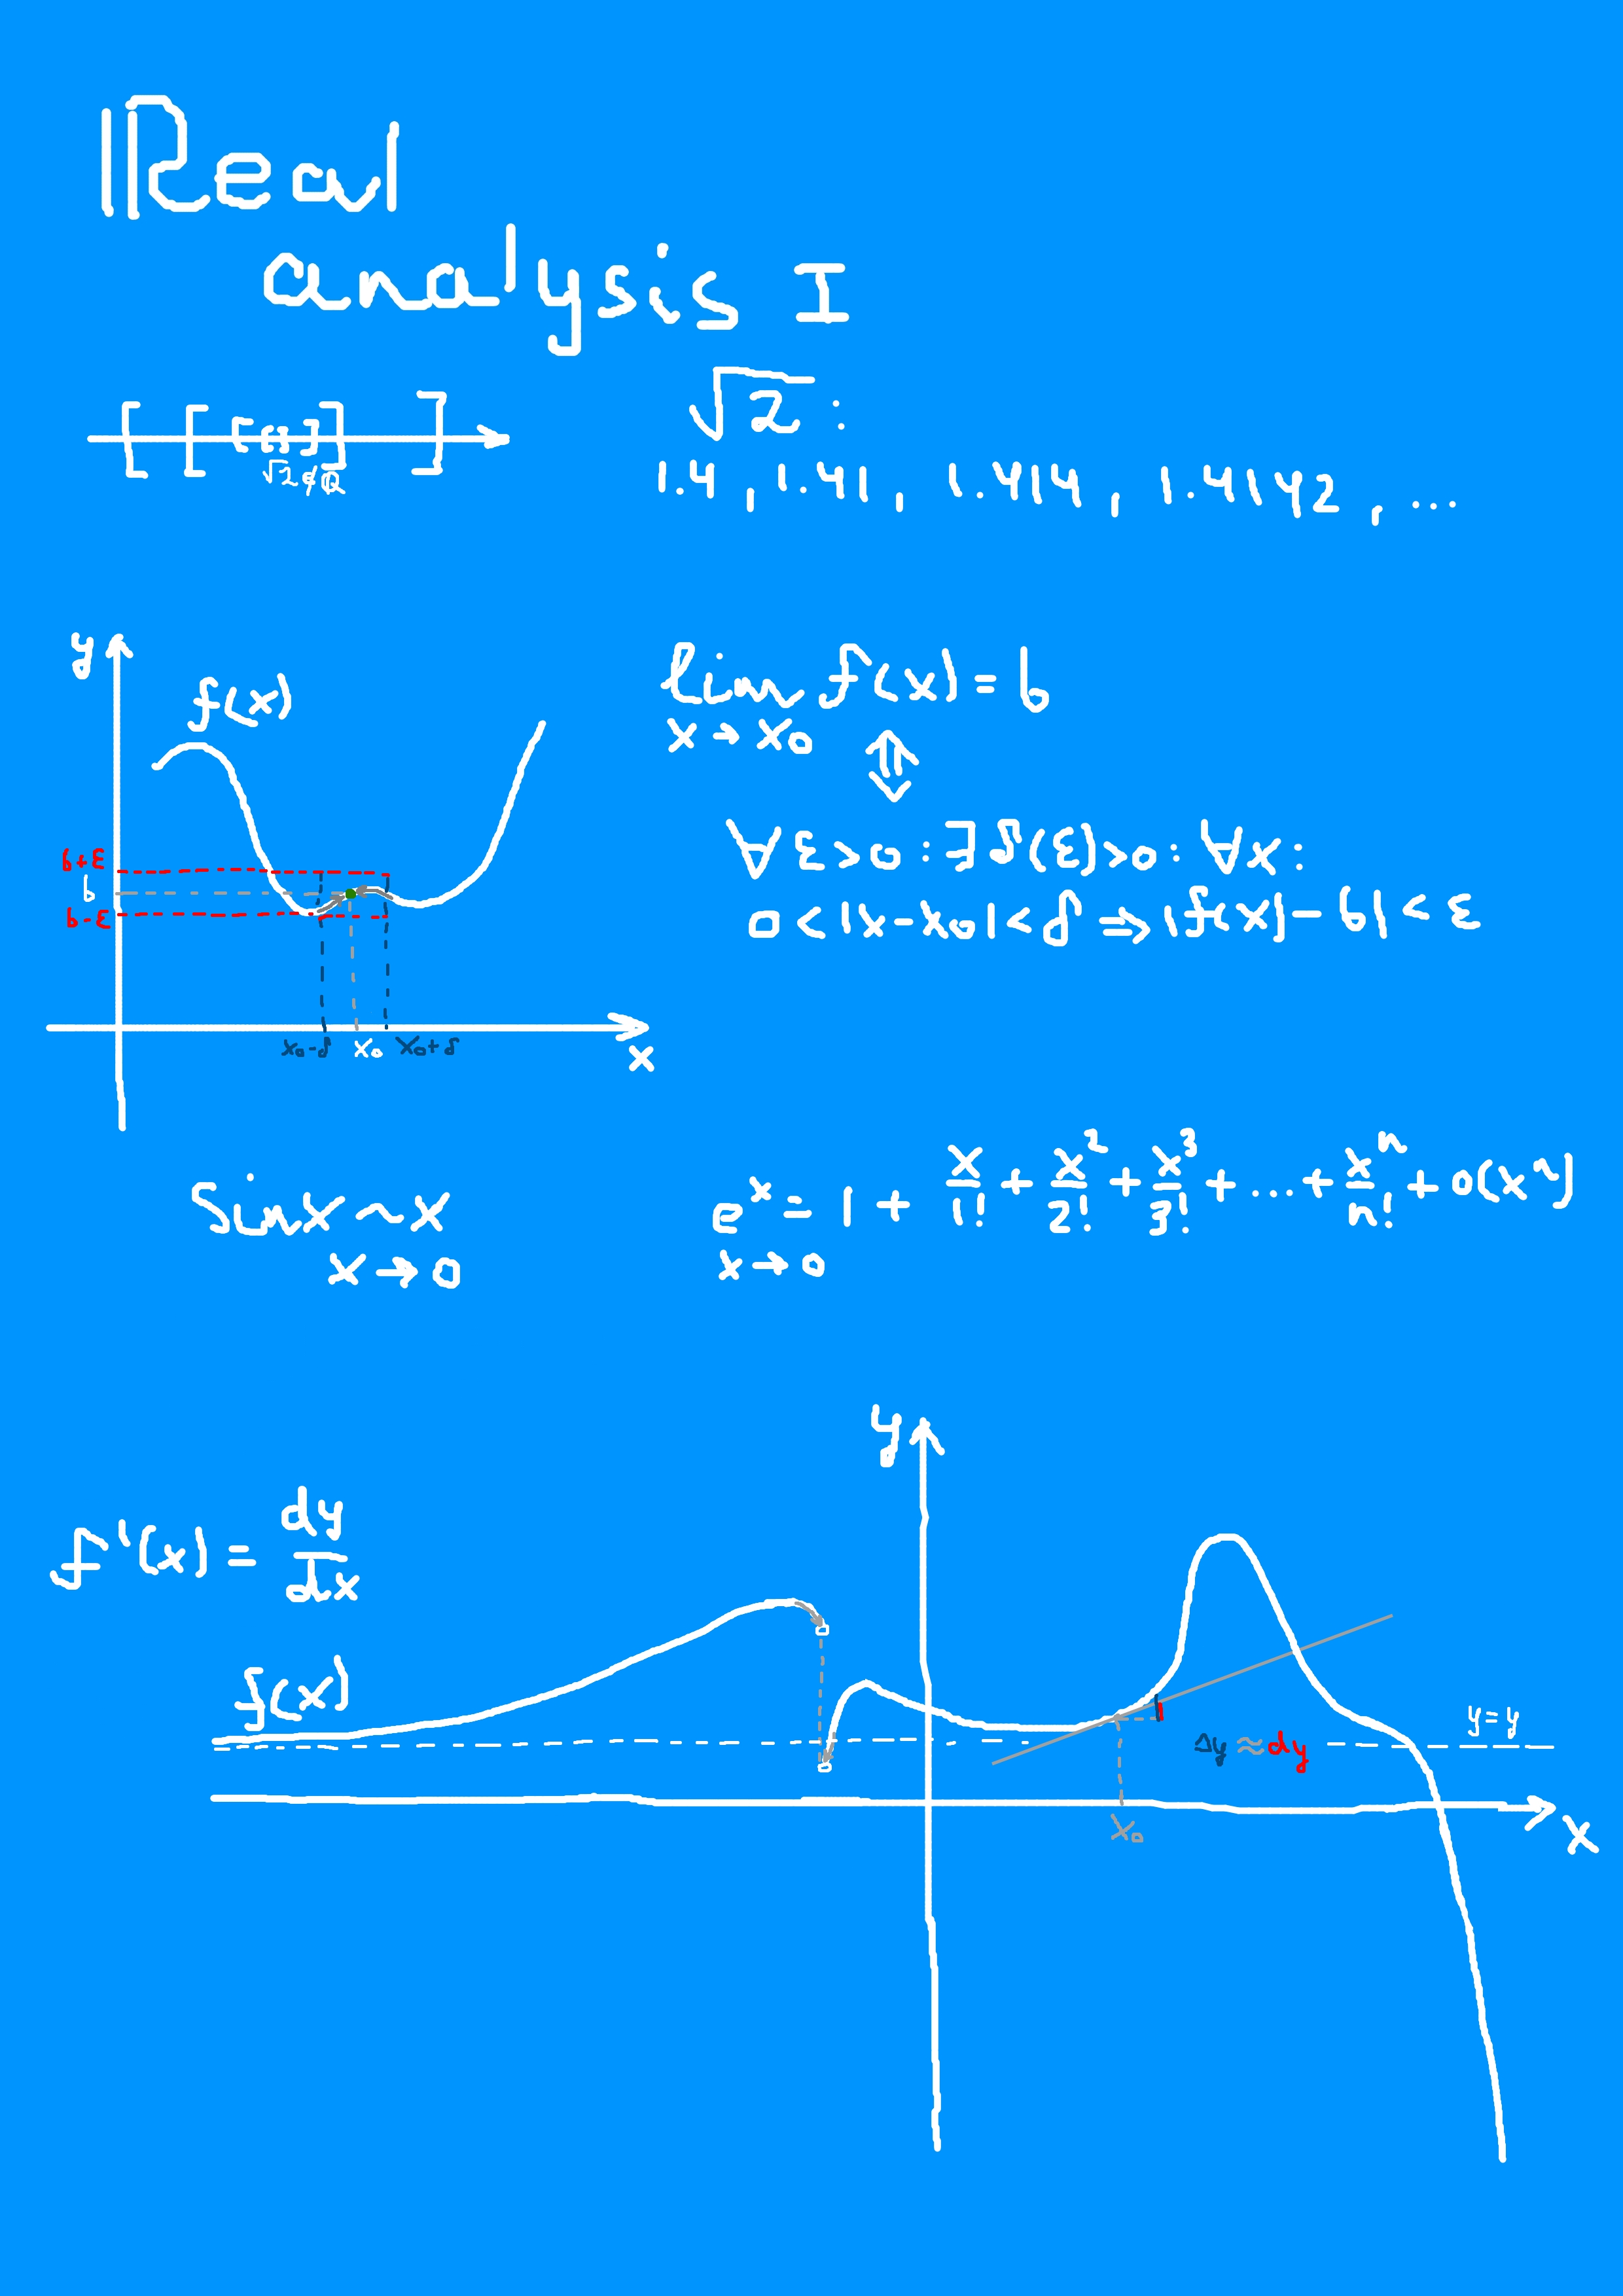
\includepdf{preview.jpg}
\tableofcontents
\newpage

%\iffalse %IMPORTANT COMMENT
	\section*{Необхідні тулзи для розвитку матана}
	\subsection*{Шкільні речі та трошки про те, як розвивати множину дійсних чисел}
	
	Уже з такими числами було більш-менш ознайомлено в школі. Починалось все з натуральних чисел:	
	$$ \mathbb{N} = \{1, \ 2, \ 3, \ \dots\} $$
	Далі пішли цілі  числа: \\
	$$ \mathbb{Z} = \{\dots,\ -3 ,\ -2, \ -1,\ 0,\ 1,\ 2,\ 3,\ \dots\} $$
	Саме в цілих числах ми змогли визначити вже операцію $+$, але цього недостатньо. Потім раціональні числа: \\
	$$ \mathbb{Q} = \left\{ \dfrac{m}{n} \biggm| m \in \mathbb{Z},\ n \in \mathbb{N} \right\} $$
	А тут вже ми змогли визначити операцію $\cdot$, і цього теж мало. Насправді, всі ці множини та операції $+,\ \cdot$ можна спробувати дуже строго формалізувати, проте цього робити не планую. Це не сильно вплине на якість вивчення матана.
	
	Настав саме час дослідити поле дійсних чисел -- $\mathbb{R}$. Одна з головних мотивацій зробити -- це прямокутний трикутник зі сторонами $1$.
	\begin{figure}[H]
	\centering
	\begin{tikzpicture}
	\draw[thick] (0,0)--(2,0) node at (-0.3,1) {$1$};
	\draw[thick] (0,0)--(0,2) node at (1,-0.3) {$1$};
	\draw[thick] (2,0)--(0,2) node at (1.2,1.2) {$x$};
	\end{tikzpicture}
	\end{figure}
	За теоремою Піфагора, ми вже знаємо, що
	$x^2 = 1^2 + 1^2 \implies x^2 = 2$. І от тут виникли проблеми:
	\begin{proposition}
	$\not\exists  x \in \mathbb{Q}: \ x^2 = 2$. Або, інакше кажучи, $\sqrt{2} \not\in \mathbb{Q}$.
	\end{proposition}
	
	\begin{proof}
	!Припустімо, що все ж таки $\exists x \in \mathbb{Q}$, тобто $x= \dfrac{m}{n}, m \in \mathbb{Z}, n \in \mathbb{N}$, нескоротимий дріб, для якого\\
	$x^2 = 2 \implies \dfrac{m^2}{n^2} = 2 \implies m^2 = 2n^2$.\\
	Оскільки $2n^2$ -- це парне число, то $m^2$ -- також парне, а тому $m$ -- парне, тоді таке число представимо у вигляді $m = 2k, k \in \mathbb{Z}$.\\
	$4k^2 = 2n^2 \implies 2k^2 = n^2$\\
	Оскільки $2k^2$ -- це парне число, то $n^2$ -- також парне, а тому $n$ -- парне, тоді таке число представимо у вигляді $n = 2l, l \in \mathbb{Z}$.\\
	Проте $m,n$ одночасно не можуть бути парними, оскільки ми отримаємо скоротимий дріб, а, за умовою, ми не брали таких. Суперечність!\\
	Отже, наше припущення було невірним.
	\end{proof}
	
	\iffalse
	\begin{theorem}
	Множина раціональних чисел $\mathbb{Q}$ -- зліченна.
	\end{theorem}

	\begin{proof}
	Нагадаю собі, що зліченною називають таку множину, де кожному числу ставиться відповідний номер. Коротше, ми можемо їх нумерувати. Вважаю, що доведення буде не самий rigorous, але тим не менш, підтвердити цей факт можна.\\
	Раціональні числа запишемо в такому порядку:
	\begin{figure}[H]
	\centering
	\begin{tikzpicture}[scale = 0.8, every node/.style={scale=0.8}]
	\foreach \y in {1,2,...,4} {
		\foreach \x in {1,...,4} {
			\node at ({2*\x},4-\y) {$\dfrac{-\x}{\y}$};
			\node at ({2*\x-1},4-\y) {$\dfrac{\x}{\y}$};
			}
			\node at (0, 4-\y) {$\dfrac{0}{\y}$};
		}
	\foreach \x in {0,1,...,8}
		\node at (\x,-1) {$\vdots$};
	\foreach \y in {0,...,3}
		\node at (9,\y) {$\dots$};
	\node at (9,-1) {$\ddots$};
	\end{tikzpicture}
	\end{figure}
	А тепер ми будемо проходитись по раціональних числам такою змійкою:
	\begin{figure}[H]
	\centering
	\begin{tikzpicture}[scale = 0.8, every node/.style={scale=0.8}]
		\draw[red, thick] (0,3)--(1,3)--(1,2)--(0,2)--(0,1)--(2,1)--(2,3)--(3,3)--(3,0)--(0,0)--(0,-1)--(4,-1)--(4,3)--(5,3)--(5,-1);
	\foreach \y in {1,2,...,4} {
		\foreach \x in {1,...,4} {
			\node at ({2*\x},4-\y) {$\dfrac{-\x}{\y}$};
			\node at ({2*\x-1},4-\y) {$\dfrac{\x}{\y}$};
			}
			\node at (0, 4-\y) {$\dfrac{0}{\y}$};
		}
	\foreach \x in {0,1,...,8}
		\node at (\x,-1) {$\vdots$};
	\foreach \y in {0,...,3}
		\node at (9,\y) {$\dots$};
	\node at (9,-1) {$\ddots$};
	\end{tikzpicture}
	\end{figure}
	І поки ми проходитимемо змійкою, ми будемо ігнорувати такі дроби, що повторюють числа. Наприклад, ми перетнули $\dfrac{1}{1}$, тоді $\dfrac{2}{2}, \dfrac{3}{3},\dots$ ігноруватимемо.\\
	Кожне число ми нумеруємо. Тобто дійсно, ми отримали, що $\mathbb{Q}$ -- зліченна множина.
	\end{proof}		
	\fi
	
	Саме це твердження є головною мотивацією розвивати нову множину. У грубому сенсі, це все означає, що множина $\mathbb{Q}$ -- неповна множина, тобто на числовій прямій є \lq\lq дірки\rq\rq. І саме $\mathbb{R}$ прибирає ці самі  \lq\lq дірки\rq\rq . \\
	Множину $\mathbb{R}$ можна конструювати як набір нескінченних десяткових дробів. Наприклад, число $\sqrt{2} = 1.41421356237\dots$ Там же можна визначити всі операції. Конструкцією $\mathbb{R}$ займемося згодом.
	
	\subsection*{Принцип математичної індукції}
	\begin{definition}
	Числова множина $E$ називається \textbf{індуктивною}, якщо
	\begin{align*}
		\forall x \in E: x+1 \in E
	\end{align*}
	\end{definition}
	
	\begin{theorem}
	Множина натуральних чисел $\mathbb{N}$ -- мінімальна індуктивна множина, що містить $1$.
	\end{theorem}
	
	\begin{remark}
	Переформулюю математичною мовою дану теорему:\\
	$\forall E$ -- індуктивна: $1 \in E \implies \mathbb{N} \subset E$.
	\end{remark}
	
	\begin{proof}
	1) Те, що $\mathbb{N}$ індуктивна, зрозуміло, тому що $\forall k \in \mathbb{N}: k+1 \in \mathbb{N}$.\\
	2) Оскільки $1 \in E$ і, більш того, вона є індуктивною, то $2 \in E, 3 \in E, \dots, k \in E$.\\
	А тому $\forall k \in \mathbb{N} \Rightarrow k \in E$. Таким чином, $\mathbb{N} \subset E$.
	\end{proof}
	
	\begin{corollary}[Принцип математичної індукції]
	Розглянемо числову множину $E = \{n \in \mathbb{N}: P(n)\}$. Тут $P(n)$ -- це деяка умова.\\
	Тоді якщо $1 \in E$ та індуктивна, то $E = \mathbb{N}$.\\
	Авторське скорочення: МІ -- математична індукція.
	\end{corollary}
	
	\begin{proof}
	За умовою наслідка, маємо, що $E \subset \mathbb{N}$. Оскільки $1 \in E$ та індуктивна, то за попередньою теоремою, $\mathbb{N} \subset E$. Отже, $E = \mathbb{N}$.
	\end{proof}
	
	\textit{Про що цей наслідок}: ми хочемо стверджитись, що $P(n)$ виконується при будь-яких $n \in \mathbb{N}$. Для цього треба зробити три кроки:\\
	\textbf{1. База індукції}\\
	Перевіряємо, що $P(1)$ виконується.
	\bigskip \\
	\textbf{2. Крок індукції}\\
	Вважаємо, що $P(n)$ -- виконано. Показуємо, що $P(n+1)$ виконується.
	\bigskip \\
	Двома кроками доводимо, що наша множина $E$ -- індуктивна, що містить одиницю. Отже, МІ доведено, а тому $P(n)$ виконується завжди.
	
	\begin{example}
	Довести, що $1 + 2 + \dots + n = \dfrac{n(n+1)}{2}$.\\
	Тут множина $E = \left\{n \in \mathbb{N}: 1 + 2 + \dots + n = \dfrac{n(n+1)}{2} \right\}$.\\
	1. База індукції\\
	$1 \in E \Rightarrow 1 = \dfrac{1(1+1)}{2} = 1$
	\bigskip \\
	2. Крок індукції\\
	Нехай $k \in E$, тобто 
	$1 + 2 + \dots + k = \dfrac{k(k+1)}{2}$\\
	Доведемо, що $k+1 \in E$\\
	$1+ 2 + \dots + k + (k+1) = \dfrac{k(k+1)}{2} + k = \dfrac{k(k+1)+2k}{2} = \dfrac{(k+1)(k+2)}{2}$\\
	Отже, $k+1 \in E$.
	А значить, $E = \mathbb{N}$, тобто наша формула виконується $\forall n \in \mathbb{N}$. МІ доведено.
	\end{example}
	
	\begin{example}
	Довести, що $\forall n \in \mathbb{N} \setminus \{1\}: 2^n \geq n$.\\
	Тут множина $E = \{n \in \mathbb{N} \setminus \{1\}: 2^n \geq n \}$.\\
	1. База індукції\\
	$2 \in E \Rightarrow 2^2 \geq 2$
	\bigskip \\
	2. Крок індукції\\
	Нехай $k \in E$, тобто $2^k \geq k$.\\
	Доведемо, що $k+1 \in E$. Маємо\\
	$2^{k+1} = 2 \cdot 2^k \geq 2k = k + k > k+1$\\
	Отже, $k+1 \in E$, тобто $E = \mathbb{N} \setminus \{1\}$, тобто наше твердження виконується $\forall n \neq 1$. МІ доведено.
	\end{example}
	
	\subsection*{Основні нерівності}
	\begin{theorem}[Нерівність Бернуллі]
	Для всіх $x > -1$ виконано $(1+x)^n \geq 1+nx, \quad \forall n \geq 1$.
	\end{theorem}
	
	\begin{proof}
	Доведення за МІ по $n$.\\
	1. База індукції: при $n=1$: $(1+x)^1 \geq 1+1\cdot x$. Нерівність виконується.\\
	2. Крок індукції: нехай для фіксованого $n$ нерівність виконується. Доведемо для значення $n+1$.\\
	$(1+x)^{n+1}=(1+x)(1+x)^n \geq (1+x)(1+nx)=1+(n+1)x+nx^2 \geq 1+(n+1)x$\\
	Отже, така нерівність справедлива $\forall n \geq 1$. \\
	МІ доведено.
	\end{proof}
	
	\begin{theorem}[Нерівність Коші]
	Для всіх $a_1,\dots,a_n > 0$ виконано
	$\dfrac{a_1+\cdots+a_n}{n} \geq \sqrt[n]{a_1 \cdots a_n}, \hspace{0.2cm} \forall n \geq 1$.
	\end{theorem}
	
	\begin{proof}
	Тимчасове перепозначення: $A_n = \dfrac{a_1+\cdots+a_n}{n}, \quad G_n = \sqrt[n]{a_1 \cdots a_n}$.\\
	Зрозуміло, що $\dfrac{A_n}{A_{n-1}} > 0 \implies \dfrac{A_n}{A_{n-1}}-1>-1$. Тоді за нерівністю Бернуллі,\\
	$\displaystyle \left(1+ \left(\frac{A_n}{A_{n-1}} -1 \right) \right)^n \geq 1 + n \cdot \left(\frac{A_n}{A_{n-1}} -1 \right)$
	$\implies \displaystyle \frac{(A_n)^n}{(A_{n-1})^n} \geq \frac{a_n}{A_{n-1}} \implies \displaystyle (A_n)^n \geq a_n (A_{n-1})^{n-1}, \forall n \geq 1$. \\ Тоді $(A_n)^n \geq a_n (A_{n-1})^{n-1} \geq \cdots \geq a_n a_{n-1} \cdots a_1$. \\ Отже, $A_n \geq G_n$, що й хотіли довести.
	\end{proof}
	
	\subsection*{Біноміальні коефіцієнти, біном Ньютона}
	\begin{definition}
	\textbf{Факторіалом натурального числа} називають таке число:
	\begin{align*}
	n! = n \cdot (n-1) \dots 2 \cdot 1
	\end{align*}
	Домовленість: $0! = 1$.
	\end{definition}
	
	\begin{corollary} 
	$(n+1)! = (n+1)n!$
	\end{corollary}
	
	\begin{definition}
	\textbf{Біноміальним коефіцієнтом} назвемо ось таке число:
	\begin{align*}
	C_n^k = \dfrac{n!}{k!(n-k)!}
	\end{align*}
	Інтерпретація того числа: серед $n$ студентів обрати $k$ студентів, що будуть відраховані. При цьому неважливо, у якому порядку $k$ студентів стануть в ряд.
	\end{definition}

	\begin{proposition}
	$C_n^k + C_n^{k+1} = C_{n+1}^{k+1}$
	\end{proposition}
	
	\begin{proof}
	$C_n^k + C_n^{k+1} = \dfrac{n!}{k!(n-k)!} + \dfrac{n!}{(k+1)!(n-(k+1))!} \boxed{=}$\\
	За властивістю факторіала, $(n-k)! = (n-k-1)!(n-k)$, а також $(k+1)! = (k+1)k!$\\
	$\boxed{=} \dfrac{n!}{k!(n-k)(n-k-1)!} + \dfrac{n!}{k!(k+1)(n-k-1)!} = \dfrac{n!}{k!(n-k-1)!} \left(\dfrac{1}{n-k} + \dfrac{1}{k+1} \right) = \\ = \dfrac{n!}{k!(n-k-1)!} \dfrac{n+1}{(n-k)(k+1)} \boxed{=}$\\
	Знову за властивістю факторіала, $(n+1)n! = (n+1)!$, а також \\ $(n-k)(n-k-1)! = (n-k)!$, $(k+1)k! = (k+1)!$ \\
	$\boxed{=} \dfrac{(n+1)!}{(k+1)!(n-k)!} = \dfrac{(n+1)!}{(k+1)!((n+1)-(k+1))!} = C_{n+1}^{k+1}$
	\end{proof}
	
	\subsubsection*{Трикутник Паскаля}
	В школі були такі формули:\\
	$(a+b) = a + b$\\
	$(a+b)^2 = a^2+2ab + b^2$\\
	$(a+b)^3 = a^3 + 3a^2b + 3ab^2 + b^3$\\
	$(a+b)^4 = ?$\\
	Приберімо зараз літери $a,b$ та отримаємо такий малюнок:
\begin{figure}[H]
\centering
	\begin{tikzpicture}
	\node at (1,1) {$1$};
	\node at (2,1) {$1$};
	\node at (0.5,0) {$1$};
	\node at (1.5,0) {$2$};
	\draw[->] (0.6,-0.2)--(0.9,-0.8);
	\draw[->] (1.4,-0.2)--(1.1,-0.8);
	\node at (2.5,0) {$1$};
	\node at (0,-1) {$1$};
	\node[red] at (1,-1) {$3$};
	\node at (2,-1) {$3$};
	\node at (3,-1) {$1$};
	\end{tikzpicture}
\end{figure}
	По краях трикутника ми будемо завжди з одиницями. Червоне число $3$ взялося шляхом додавання двох чисел зверху: $1 + 2$. Якщо дотримуватись аналогічних міркувань, то ми зможемо розширити трикутник Паскаля:
\begin{figure}[H]
\centering
	\begin{tikzpicture}
	\node at (1,1) {$1$};
	\node at (2,1) {$1$};
	\node at (0.5,0) {$1$};
	\node at (1.5,0) {$2$};
	\node at (2.5,0) {$1$};
	\node at (0,-1) {$1$};
	\node at (1,-1) {$3$};
	\node at (2,-1) {$3$};
	\node at (3,-1) {$1$};
	
	\node[blue] at (-0.5,-2) {$1$};
	\node[blue] at (0.5,-2) {$4$};
	\node[blue] at (1.5,-2) {$6$};
	\node[blue] at (2.5,-2) {$4$};
	\node[blue] at (3.5,-2) {$1$};
	
	\node at (-1,-3) {$1$};
	\node at (0,-3) {$5$};
	\node at (1,-3) {$10$};
	\node at (2,-3) {$10$};
	\node at (3,-3) {$5$};
	\node at (4,-3) {$1$};
	\node at (1.5,-4) {$\dots$};
	\end{tikzpicture}
	\caption*{Трикутник Паскаля}
\end{figure}
	Із цього трикутника ми тепер можем знайти $(a+b)^4$, якщо знати, як повернути літери:\\
	$(a+b)^4 = \textcolor{blue}{1} a^4 + \textcolor{blue}{4}a^3 b + \textcolor{blue}{6} a^2  b^2 + \textcolor{blue}{4}a b^3 + \textcolor{blue}{1} b^4$\\
	Формула починається з $a^4$ та $b^0$. А далі степінь $a$ зменшуємо на одиницю, а степінь $b$, навпаки, збільшуємо на одиницю. А тепер узагальнімо це:
	
	\begin{theorem}[Біном Ньютона]
	$(a+b)^n = C_n^0 a^n b^0 + C_n^1 a^{n-1}b + C_n^2 a^{n-2}b^2 + \dots + C_n^{n-1} a b^{n-1} + C_n^n a^0 b^n$.\\
	Якщо коротко, можна записати як $(a+b)^n = \displaystyle \sum_{k=0}^n C_n^k a^{n-k} b^k$.
	\end{theorem}
	
	\begin{proof}
	Дану формулу доведемо за МІ по числу $n \in \mathbb{N}$.\\
	1. База індукції. $n = 1 \implies (a+b)^1 = C_1^0 a^1 b^0 + C_1^1 a^0 b^1 = a + b$\\
	2. Крок індукції. Припустимо, що для фіксованого $n$ формула виконана, тобто $(a+b)^n = \displaystyle\sum_{k=0}^n C_n^k a^{n-k} b^k$. Перевіримо цю формулу для $n+1$.\\
	$(a+b)^{n+1} = (a+b)(a+b)^n \overset{\textrm{припущення МІ}}{=} (a+b) \displaystyle \sum_{k=0}^n C_n^k a^{n-k} b^k = \sum_{k=0}^n C_n^k a^{n-k+1} b^k + \sum_{k=0}^n C_n^k a^{n-k} b^{k+1} = \textcolor{red}{a^{n+1}} + \sum_{\textcolor{red}{k=1}}^n C_n^k a^{n-k+1} b^k + \sum_{k=0}^{\textcolor{red}{n-1}} C_n^k a^{n-k} b^{k+1} + \textcolor{red}{b^{n+1}} \boxed{=}$\\
	В другій сумі ми замінимо лічильник: $m = k+1$\\
	Було: $0,1,2,\dots, n-1$\\
	Стало: $1,2,3,\dots,n$\\
	$\boxed{=} a^{n+1} + \displaystyle \sum_{k=1}^n C_n^k a^{n-k+1}b^k + \sum_{m=1}^n C_n^{m-1} a^{n-(m-1)}b^{(m-1)+1} + b^{n+1} \boxed{=}$ \\
	Замінимо літеру $m = k$, сума від цього не зміниться\\
	$\boxed{=} a^{n+1} + \displaystyle \sum_{k=1}^n C_n^k a^{n-k+1}b^k + \sum_{k=1}^n C_n^{k-1} a^{n-k+1}b^{k} + b^{n+1}
	= a^{n+1} + \sum_{k=1}^n a^{n-k+1}b^k \left(C_n^k + C_n^{k-1} \right) + b^{n+1}  = a^{n+1} + \sum_{k=1}^n a^{n-k+1}b^k C_{n+1}^k + b^{n+1}
	= C_{n+1}^0 a^{n+1} b^0 + \sum_{k=1}^n a^{n-k+1}b^k C_{n+1}^k + C_{n+1}^{n+1} a^0 b^{n+1} = \sum_{k=0}^{n+1} C_{n+1}^k a^{n-k+1}b^k  = (a+b)^{n+1}$\\
	МІ доведено.
	\end{proof}
	\newpage
	%\fi %IMPORTANT COMMENT
    \iffalse %IMPORTANT COMMENT
    
	\section{Множина дійсних чисел}
	\iffalse
	Мабуть, трошки треба зробити вступ до множини $\mathbb{Q}$, щоб стало ясніше. Про те, як їх додавати, віднімати, множити, ділити, уже відомо зі школи. Але суттєвим є ось таке твердження:
	\begin{theorem}
	$x \in \mathbb{Q} \iff x$ має період в розкладі десяткового дробу.
	\end{theorem}
	
	\begin{proof}
	\rightproof Дано: $x \in \mathbb{Q}$, тобто $x = \dfrac{a}{b}$ - нескоротимий правильний дріб (якщо це просто ціле число, то тут нема що робити). Запишемо в вигляді десяткового дробу.\\
	Ми маємо наразі $a < b$, але можна знайти такий $n \in \mathbb{N}$, для якого $10^n a > b$. Далі ділимо $10^n a$ на $b$ за алгоритм Евкліда, отримаємо $10^n a = q b + r_1$, причому $0 \leq r_1 < b$.\\
	Далі розглянемо аналогічно $\dfrac{r_1}{b}$, маємо $r_1 < b$, але можна знайти такий $n_1 \in \mathbb{N}$, для якого $10^{n_1} r_1 > b$. Далі ділимо $10^{n_1} r_1$ на $b$ за алгоритм Евкліда, отримаємо $10^{n_1} r_1 = q_1 b + r_2$, причому $0 \leq r_2 < b$.\\
	Далі розглянемо аналогічно $\dfrac{r_2}{b}$ та робимо все аналогічно...\\
	Призупинимось на $r_k$ тимчасово та розпишемо $\dfrac{a}{b}$ як десятковий дріб:\\
	$\dfrac{a}{b} = \dfrac{q}{10^n} + \dfrac{r_1}{b 10^n} = \dfrac{q}{10^n} + \dfrac{q_1}{10^{n+n_1}} + \dfrac{r_2}{b 10^{n+n_1}} = \dots = \\ = \dfrac{q}{10^n} + \dfrac{q_1}{10^{n+n_1}} + \dfrac{q_2}{10^{n+n_1+n_2}} + \dots + \dfrac{q_{k-1}}{ 10^{n+n_1+n_2+\dots + n_{k-1}}} + \dfrac{r_k}{b 10^{n+n_1+n_2+\dots + n_{k-1}}} = \\
	= \underbrace{0.0\dots 0}_{n\text{ разів}} q + \underbrace{0.0\dots 0}_{n+n_1\text{ разів}} q_1 + \dots + \underbrace{0.0\dots 0}_{n+n_1+\dots+n_{k-1}\text{ разів}}q_{k-1} + \dfrac{r_k}{b 10^{n+n_1+\dots+n_{k-1}}}$.\\
	У результаті рано чи пізно у нас виникне така картина, що отримаємо $r_k$, а після повторної ітерації можемо отримати $r_i$ при $i < k$. Це можливо, тому що всі $0 \leq r < b$, відповідно вибір в нас скінченний. А коли ми отримаємо $r_i$, то далі відбувається зациклення: буде $r_{i+1},r_{i+2}, \dots, r_k, r_{i+1}, r_{i+2}, \dots$\\
	Тоді отримаємо $\dfrac{r_k}{b} = \dfrac{q_k}{10^{n_k}} + \dfrac{r_i}{b 10^k}$, але ми ВЖЕ знаємо, чому це дорівнює за попередніми ітераціями:\\
	$\dfrac{r_i}{b} = \dfrac{q_i}{10^{n_i}} + \dfrac{q_{i+1}}{10^{n_i+n_{i+1}}} + \dots + \dfrac{q_k}{10^{n_i + n_{i+1} + \dots + n_k}} + \dfrac{r_i}{b 10^{n_i + n_{i+1} + \dots + n_k}}$.\\
	У результаті, ми будемо рекурсивно постійно підставляти значення $\dfrac{r_k}{b}$ -- отримаємо таким чином нескінченний десятковий дріб, що є періодичним:\\
	$x = 0.0\dots 0 q_1 0 \dots q_2 0 \dots 0 \overline{q_i 0 \dots 0 q_{i+1} 0 \dots 0 q_k}$ (перевірити ще раз)
	\bigskip \\
	\leftproof Дано: $x$ десятковий дріб з періодом, тобто наразі $x = a_0.a_1 \dots a_k \overline{b_1 \dots b_p}$. Тоді\\
	$10^k x = 10^k a_0 + a_1 \dots a_k.\overline{b_1 \dots b_p}$.\\
	$10^{k+p} x = 10^{k+p} a_0 + a_1 \dots a_k b_1 \dots b_k. \overline{b_1 \dots b_p}$.\\
	Друге рівняння віднімемо від першого та отримаємо:\\
	$(10^{k+p} - 10^k)x = (10^{k+p} - 10^k)a_0 + (a_1 \dots a_k b_1 \dots b_p - a_1 \dots a_k)$.\\
	$x = \dfrac{a_1 \dots a_k b_1 \dots b_k - a_1 \dots a_k}{10^{k+p} - 10^k} \in \mathbb{Q}$.
	\end{proof}
	
	Висновок: числа, які ми будемо розглядати далі, вони не матимуть період.
	\fi
	
	\subsection{Числова вісь}
	\begin{definition}
	\textbf{Числовою віссю} ми будемо називати вісь, де задається точка, що є початком координат, а також масштаб виміру.
	\begin{figure}[H]
	\centering
	\begin{tikzpicture}
	\draw[thick, ->] (-5,0)--(5,0);
	\fill (0,0) circle (1pt) node[anchor = north] {$O$};
	\fill (1,0) circle (1pt) node[anchor = north] {$I$};
	\end{tikzpicture}
	\caption*{Тут стоїть початок координат $O$. Йому будемо ставити в відповідність число $0$. Ми задали одиничний масштаб, тому точці $I$ відповідатиме число $1$.}
	\end{figure}
	\end{definition}

Ми далі цей відрізок $OI$ будемо відкладати праворуч -- отримаємо точки, що відповідають натуральним числам.\\
Після цього симетрично відносно початку відкладаємо всі отримані точки -- отримаємо вже цілі числа. Загалом числова вісь виглядатиме так:
	\begin{figure}[H]
	\centering
	\begin{tikzpicture}
	\draw[thick, ->] (-5,0)--(5,0);
	\foreach \i in {-4,-3,...,4}
		\fill (\i,0) circle(1pt) node[anchor = north] {$\i$};
	\end{tikzpicture}
	\end{figure}
	Тепер з'ясуємо, як можна розташувати додатне раціональне число $\dfrac{m}{n}$ (це буде правильний дріб із взаємно простими числами). Для початку відрізок $OI$ необхідно розбити на $n$ рівних частин. Це можна зробити ось так: проводимо довільну пряму через т. $O$, позначаємо якусь точку на неї, відкладаємо $n$ разів; останню точку сполучаємо з т. $I$, а далі просто паралельним чином проводимо інші прямі. На основі фактів з планиметрії, ми змогли розділити.
	\begin{figure}[H]
	\centering
	\begin{tikzpicture}
	\draw[thick] (0,0)--(2,0);
	\fill (0,0) circle (1pt) node[anchor = north] {$O$};
	\fill (2,0) circle (1pt) node[anchor = north] {$I$};
	
	\foreach \i in {1,2,3,4} {
		\fill[blue] ({0.75*\i},{0.5*\i}) circle (1pt);
		\draw ({0.75*\i},{0.5*\i})--({\i/2.0},0);
	}
		
	\draw[blue] (-1,{-2/3}) -- (4,{2+2/3});
	\end{tikzpicture}
	\end{figure}
	Отримали відрізок довжиною $\dfrac{1}{n}$. А далі відкладаємо праворуч $m$ разів.\\
	Тепер постає питання, що робити з ірраціональними числами. Ми вже знаємо, що будь-яке раціональне число можна записати як нескінченний десятковий дріб з періодом (ті числа, що скінченні, все одно можна записати в нескінченному вигляді: $0.5 = 0.5(0)$). Тобто на числовій вісі лежать всі десяткові дроби з періодом. Тепер ми хочемо додати десяткові дроби, що НЕ мають період взагалі. Один з прикладів -- це як раз таки $\sqrt{2} = 1.41421356237 \dots$\\
	Отже, ми хочемо в будь-якій точці $x$ на числовій прямій поставити в відповідність деякий десятковий дріб.
	
	\subsection{Основні визначення}
	\begin{definition}
	\textbf{Дійсним числом} назвемо такий об'єкт:
	\begin{align*}
	x = \pm \alpha_0.\alpha_1 \alpha_2 \dots \alpha_n \dots,
	\end{align*}
	де $\alpha_0 \in \mathbb{N} \cup \{0\}$, а решта $\alpha_i$ -- це цифри, тобто $\alpha_i \in \{0,1,2,3,4,5,6,7,8,9\}$.\\
	Позначення: $\mathbb{R}$ -- множина всіх дійсних чисел. Тобто тут $x \in \mathbb{R}$.
	\end{definition}
	
	\begin{example}
	Зокрема $\sqrt{2} = +1.41421356237 \dots$ -- один з прикладів дійсних чисел.
	\end{example}
	
	Тепер виникає питання, як дійсне число можна розташувати на числову вісь.\\
	Розглянемо число $x = \alpha_0.\alpha_1\alpha_2 \dots$
	\begin{figure}[H]
	\centering
	\begin{tikzpicture}
	\draw[thick, ->] (-5,0)--(5,0);
	\foreach \i in {-4,-3,...,4}
		\fill (\i,0) circle(1pt) node[anchor = north] {$\i$};
	\fill (3.56431,0) circle(1pt) node[anchor = north] {$x$};
	\end{tikzpicture}
	\end{figure}
	У нас задано одиницю $1$, що відповідає відрізку $OI$. Ми цей відрізок будемо накладати $\alpha_0 + 1$ разів. У нас буде залишок $L_1$, довжина якої менша за $1$.\\
	Далі розглядаємо відрізок $OI_1$, що відповідає довжині $\dfrac{1}{10}$. Накладаємо $OI_1$ на залишок $L_1$ разів $\alpha_1 + 1$. У нас буде залишок $L_2$, довжина якої менша за $0.1$.\\
	\vdots \\
	Далі цей процес продовжується або скінченне число разів, або буде необмежене число разів (зокрема для числа $\dfrac{4}{3}$ цей процес нескінченний).
	
	\begin{remark}
	$0 \in \mathbb{R}$, ми можемо розписати $0 = +0.000 \dots$ або $0 = -0.000 \dots$
	\end{remark}
	
	\begin{remark}
	Будь-яке раціональне число $q \in \mathbb{Q}$ автоматично $q \in \mathbb{R}$, тому що відомо зі школи, що $q$ можна записати або як скінченний десятковий дріб (це можна інтерпретувати як десятковий дріб з нескінченною кількістю нулів), або нескінченний десятковий дріб з періодом.\\
	Таким чином, $\mathbb{Q} \subset \mathbb{R}$.
	\end{remark}
	
	\begin{definition}
	Число $x \in \mathbb{R}$ називається \textbf{додатним}, якщо $\alpha_0$ має знак $+$, а також
	\begin{align*}
	\exists n \geq 0: \alpha_n > 0
	\end{align*}
	Позначення: $x > 0$.\\
	У протилежному випадку $x$ називається \textbf{недодатним}. Позначення: $x \leq 0$.
	\end{definition}
	
	\begin{remark}
	Зазвичай для додатних чисел знак $+$ писати необов'язково.
	\end{remark}

	\begin{definition}
	Число $x \in \mathbb{R}$ називається \textbf{від'ємним}, якщо $\alpha_0$ має знак $-$, а також
	\begin{align*}
	\exists n \geq 0: \alpha_n > 0
	\end{align*}
	Позначення: $x < 0$.\\
	У протилежному випадку $x$ називається \textbf{невід'ємним}. Позначення: $x \geq 0$.
	\end{definition}
	
	\begin{remark}
	Можна зауважити, що $0 \in \mathbb{R}$ буде недодатним та невід'ємним одночасно. Тому коли будемо розписувати $0 = 0.000 \dots$, знак $\pm$ опускатимемо.
	\end{remark}
	
	\begin{definition}
	Задані $x,y \in \mathbb{R}$ тобто $x = \pm \alpha_0.\alpha_1 \alpha_2 \dots$ та $y = \pm \beta_0.\beta_1 \beta_2 \dots$\\
	Числа $x,y$ називатимуться \textbf{рівними}, якщо або
	\begin{align*}
	\forall n \in \mathbb{N} \cup \{0\}: \alpha_n = \beta_n
	\end{align*}
	або
	\begin{align*}
	\exists n \in \mathbb{N} \cup \{0\}: \alpha_k = \beta_k \text{ при } 0 \leq k < n, \\ \alpha_n = \beta_n + 1, \\\alpha_m = 0, \beta_m = 9 \text{ при } m > n
	\end{align*}
	І при цьому їхні знаки збігатимуться.\\
	Позначення: $x = y$.\\
	У протилежному випадку вони будуть \textbf{нерівними}. Позначення: $x \neq y$.
	\end{definition}
	
	Друга умова може трошки спантеличити, але на прикладі буде простіше.
	
	\begin{example}
	Зокрема $0.25$ та $0.24999 \dots$ будуть вважатись однаковими. Із інтуїтивної точки зору, коли ми збільшуємо кількість цифр $9$, то ми наближаємось до $0.25$ все ближче й ближче.
	\end{example}
	
	\begin{example}
	Більш вагома мотивація, чому ми домовляємось про такі записи:\\
	$\dfrac{1}{3} = 0.333 \dots$.\\
	Якщо припустити, що ми навчились множити нескінченні десяткові дроби, то після множення на $3$ обидві частини, отримаємо:\\
	$1 = 0.999 \dots$
	\end{example}
	
	\begin{definition}
	Задані $x = \pm\alpha_0.\alpha_1 \alpha_2 \dots$ та $y = \pm\beta_0.\beta_1 \beta_2 \dots$.\\
	Якщо $x > 0, y > 0$, то будемо казати, що $x$ \textbf{менший за} $y$ (або $y$ \textbf{більший за} $x$), якщо
	\begin{align*}
	\exists n \in \mathbb{N} \cup \{0\}: \alpha_k = \beta_k \text{ при } 0 \leq k < n \\
	\alpha_n < \beta_n
	\end{align*}
	Позначення: $x < y$ (або $y > x$).\\
	Якщо $x < 0, y > 0$, то будемо завжди казати, що $x < y$.\\
	Якщо $x < 0, y < 0$, у нас тоді $x = -\alpha_0.\alpha_1 \alpha_2 \dots$ та $y = -\beta_0.\beta_1 \beta_2 \dots$ Ми будемо казати, що $x < y$, якщо, взявши числа $x' = +\alpha_0.\alpha_1 \alpha_2 \dots, y' = +\beta_0.\beta_1 \beta_2 \dots$, ми отримаємо $x' > y'$.
	\begin{figure}[H]
	\centering
	\begin{tikzpicture}
	\draw[thick, ->] (-4,0)--(4,0);
	\fill (0,0) circle(1pt) node[anchor = north] {$0$};
	\fill (2,0) circle(1pt) node[anchor = north] {$x$};
	\fill (3,0) circle(1pt) node[anchor = north] {$y$};
	\end{tikzpicture}
	\caption*{Випадок $x > 0, y > 0$.}
	\end{figure}
	\begin{figure}[H]
	\centering
	\begin{tikzpicture}
	\draw[thick, ->] (-4,0)--(4,0);
	\fill (0,0) circle(1pt) node[anchor = north] {$0$};
	\fill (-2,0) circle(1pt) node[anchor = north] {$x$};
	\fill (1,0) circle(1pt) node[anchor = north] {$y$};
	\end{tikzpicture}
	\caption*{Випадок $x < 0, y > 0$.}
	\end{figure}
	\begin{figure}[H]
	\centering
	\begin{tikzpicture}
	\draw[thick, ->] (-4,0)--(4,0);
	\fill (0,0) circle(1pt) node[anchor = north] {$0$};
	\fill (-3,0) circle(1pt) node[anchor = north] {$x$};
	\fill (-2,0) circle(1pt) node[anchor = north] {$y$};
	\fill[red] (3,0) circle(1pt) node[anchor = north] {$x'$};
	\fill[red] (2,0) circle(1pt) node[anchor = north] {$y'$};
	\end{tikzpicture}
	\caption*{Випадок $x < 0, y < 0$.}
	\end{figure}
	\end{definition}
	
	\begin{lemma}[Коректність нерівності]
	Задано $a = \alpha_0.\alpha_1 \alpha_2 \dots$ -- невід'ємне число та $b \in \mathbb{Q}$, вона має дві репрезентації: $b' = \beta_0.\beta_1\dots \beta_n 00\dots$ та $b'' = \beta_0.\beta_1\dots (\beta_n-1) 99 \dots$.\\
	$a < b' \iff a < b''$ \quad $a > b' \iff a > b''$.
	\end{lemma}
	
	\begin{remark}
	Після даної леми ми можемо надалі не розглядати числа, що містять $(9)$.
	\end{remark}
	
	\begin{proof}
	\rightproof Дано: $a < b'$, тобто існує $k \in \mathbb{N} \cup \{0\}$, для якого $\alpha_0 = \beta_0, \dots \alpha_{k-1} = \beta_{k-1}, \alpha_k < b_k$.\\
	Якщо $k > n$, то $\beta = 0$ за умовою, тобто $\alpha_k < 0$, що взагалі неможливо для цифри $\alpha_k$. Тобто маємо тоді випадок $k \leq n$.\\
	При $k = n$ маємо $\alpha_n < \beta_n$, а це еквівалентно $\alpha_n \leq \beta_n-1$.\\
	Якщо $\alpha_n < \beta_n - 1$, тоді за означенням, $a < b''$.\\
	Якщо $\alpha_n = \beta_n - 1$, то тоді серед $\alpha_{n+p}, p \geq 1$ має знайтись цифра, що не є дев'яткою. Бо якби всі $\alpha_{n+p} = 9$, то отримали би рівність $a = b'' = b'$, що неможливо, за умовою. Отже, тоді за означенням, $a < b''$.\\
	При $k < n$ теж зрозуміло автоматично, що $a < b''$.
	\bigskip \\
	\leftproof Дано: $a < b''$, тобто існує $k \in \mathbb{N} \cup \{0\}$, для якого $\alpha_0 = \beta_0, \dots, \alpha_{k-1} = \beta_{k-1}, \alpha_k < \beta_k$.\\
	Якщо $k > n$, то буде $\alpha_n = \beta_n - 1 < \beta_n$, а тому звідси $a < b'$.\\
	Якщо $k = n$, то буде $\alpha_n < \beta_n - 1 < \beta_n$, а тому звідси $a < b'$.\\
	Якщо $k < n$, то зрозуміло, що $a < b'$.
	\end{proof}
	
	\begin{remark}
	Якщо взяти довільні числа $a,b \in \mathbb{R}$, то в нас є лише одна з трьох опцій: \\ або $a = b$, або $a > b$, або $a < b$.
	\end{remark}
	
	\begin{remark}
	$a \leq b \iff \left[ \begin{gathered} a < b \\ a = b \end{gathered} \right.$
	\end{remark}
	
	\subsection{Важливі твердження}
	\begin{theorem}[Аксіома Архімеда]
	Для кожного числа $a \in \mathbb{R}$ існує число $m \in \mathbb{N}$, для якого $m > a$.
	\end{theorem}
	
	\begin{proof}
	Маємо додатне $a \in \mathbb{R}$, тобто $a = \alpha_0.\alpha_1 \alpha_2 \dots > 0$. Покладемо $m = \alpha_0 + 1$. Тоді зрозуміло, що $m > a$ та $m \in \mathbb{N}$. При $a \leq 0$ можна взяти число $m = 1$.
	\begin{figure}[H]
	\centering
	\begin{tikzpicture}
	\draw[thick, ->] (-0.5,0)--(4,0);
	\fill (0,0) circle(1pt) node[anchor = north] {$0$};
	\fill (2,0) circle(1pt) node[anchor = north] {$3$};
	\fill (2.563,0) circle(1pt) node[anchor = north] {$a$};
	\fill[red] (3,0) circle(1pt) node[anchor = north west] {$m = 4$};
	\end{tikzpicture}
	\qquad
	\begin{tikzpicture}
	\draw[thick, ->] (-3.5,0)--(1.2,0);
	\fill (0,0) circle(1pt) node[anchor = north] {$0$};
	\fill (-2.563,0) circle(1pt) node[anchor = north] {$a$};
	\fill[red] (1,0) circle(1pt) node[anchor = north] {$m = 1$};
	\end{tikzpicture}
	\end{figure}
	\end{proof}
	
	\begin{theorem}
	Нехай $a,b \in \mathbb{R}$, причому $a < b$. Тоді на інтервалі $(a,b)$ знайдеться раціональне число $q \in \mathbb{Q}$. 
	\end{theorem}
	
	\begin{proof}
	Нехай $a,b \in \mathbb{R}$ -- невід'ємні, $a = \alpha_0.\alpha_1 \alpha_2 \dots$ та $b = \beta_0.\beta_1 \beta_2 \dots$\\
	Оскільки $a < b$, то звідси $\alpha_0 = \beta_0, \dots, \alpha_{m-1} = \beta_{m-1}$, але $\alpha_m < \beta_m$.\\
	Нехай $k$ -- найменший номер, де $k > m$ та при цьому $\alpha_k < 9$. \\
	Покладемо $q = \alpha_0.\alpha_1 \dots \alpha_m \alpha_{m+1} \dots \alpha_{k-1}(\alpha_k+1)$. Зауважимо, що $q \in \mathbb{Q}$, а також $a < q < b$.\\
	Тепер нехай $a < 0$, тоді при $b > 0$ маємо раціональне число $0$. \\
	При $b \leq 0$ ми розглядаємо числа $a',b'$, що були сконструйовані як $a,b$ з протилежним знаком. Тоді матимемо інтервал $(b',a')$, там раціональне число $q \in \mathbb{Q}$ вже існує. Але тоді число $-q \in (a,b)$.
	\end{proof}

%Not correct proof, because we don't know how to multiply both sides
\iffalse
	\begin{corollary}
	Задано такі два числа $a,b \in \mathbb{R}$, що $a < b$. Тоді на інтервалі $(a,b)$ знайдеться принаймні одне ірраціональне число $x \in \mathbb{R} \setminus \mathbb{Q}$.
	\end{corollary}
	
	\begin{proof}
	Оскільки $a < b$, то звідси $\dfrac{a}{\sqrt{2}} < \dfrac{b}{\sqrt{2}}$. За попереднім наслідком, $\exists q \in \mathbb{Q}: \dfrac{a}{\sqrt{2}} < q < \dfrac{b}{\sqrt{2}}$.\\
	Тоді якщо $x = q \sqrt{2}$, то звідси $a < x < b$. А число $x \in \mathbb{R} \setminus \mathbb{Q}$, бо квадратний корінь є ірраціональним.
	\end{proof}
\fi
	
	\begin{theorem}
	Для кожного числа $a \in \mathbb{R}$ та для кожного $n \in \mathbb{N}$ знайдуться числа $q_1, q_2 \in \mathbb{Q}$, для яких $q_1 \leq a \leq q_2$, а також $q_2 - q_2 \leq \dfrac{1}{10^n}$.
	\end{theorem}
	
	\begin{proof}
	Випадок $a \in \mathbb{Q}$, можна взагалі покласти $q_1 = q_2 = 0$. Все працює.\\
	Випадок $a \geq 0, a \in \mathbb{R} \setminus \mathbb{Q}$. Маємо число $a = \alpha_0.\alpha_1 \alpha_2 \dots$ Тоді можна покласти\\
	$q_1 = \alpha_0.\alpha_1 \dots \alpha_n$ \quad $q_2 = q_1 + \dfrac{1}{10^n}$.\\
	Нерівність $q_1 \leq a \leq q_2$ зрозуміло, що виконується, а також $q_2 - q_1 = \dfrac{1}{10^n}$.\\
	Випадок $a < 0, a \in \mathbb{R} \setminus \mathbb{Q}$. Візьмемо число $b = -\alpha_0.\alpha_1 \alpha_2 \dots$. Тепер тут $b > 0$, а для нього вже довели, що існують $q_1,q_2 \in \mathbb{Q}$, для яких $q_1 \leq b \leq q_2$, а також $q_1 - q_2 \leq \dfrac{1}{10^n}$. Тоді з цього випливає, що $-q_2 \leq a \leq -q_1$.
	\end{proof}
	
	\subsection{Точкові межі}
\begin{definition}
Задано множини $A,B \subset \mathbb{R}$.\\
	Множина $A$ називається \textbf{обмеженою зверху}, якщо
	\begin{align*}
	\exists c \in \mathbb{R}: \forall a \in A: a \leq c
	\end{align*}
	Множина $B$ називається \textbf{обмеженою знизу}, якщо
	\begin{align*}
	\exists d \in \mathbb{R}: \forall b \in B: b \geq d
	\end{align*}
\end{definition}
	Множину всіх чисел, що обмежують множину зверху, позначу за $\text{Up}A$, тобто
	\begin{align*}
	\text{Up}A = \{c \in \mathbb{R}: \forall a \in A: a \leq c \}
	\end{align*}
	Множину всіх чисел, що обмежують множину зверху, позначу за $\text{Down}B$, тобто
	\begin{align*}
	\text{Down}B = \{d \in \mathbb{R}: \forall b \in B: b \geq d \}
	\end{align*}
	
	\begin{definition}
	Задано множини $A,B \subset \mathbb{R}$.\\
	Елемент $a \in A$ називається \textbf{найбільшим елементом} множини $A$, якщо
	\begin{align*}
	\forall \tilde{a} \in A: a \geq \tilde{a}
	\end{align*}
	Позначення: $a = \max A$.\\
	Елемент $b \in B$ називається \textbf{найменшим елементом} множини $B$, якщо
	\begin{align*}
	\forall \tilde{b} \in B: b \leq \tilde{b}
	\end{align*}
	Позначення: $b = \min B$.
	\end{definition}
	
	\begin{remark}
	Якщо $A \subset \mathbb{R}$ -- скінченна множина, то гарантовано існують найбільший та найменший елементи. Якщо $A \subset \mathbb{R}$ -- нескінченна множина, то там не гарантується існування.
	\end{remark}
	
	\begin{example}
	Задано множину $A = \{1-2^{-n} | n \in \mathbb{N}\} = \left\{\dfrac{1}{2}, \dfrac{3}{4}, \dfrac{7}{8}, \dots \right\}$. Вона є:\\
	обмеженою зверху числом $2 \in \mathbb{R}$, тобто $\forall a \in A: a < 2$;\\
	обмеженою знизу числом $0 \in \mathbb{R}$, тобто $\forall a \in A: a > 0$.
	\begin{figure}[H]
	\centering
	\begin{tikzpicture}[scale = 4]
	\draw[thick,->] (-0.1,0)--(2.1,0);
	%\draw[red] (1,-1pt)--(1,1pt) node at (1,-0.1) {$1$};
	\draw[red] ({1/2},-1pt)--({1/2},1pt) node at ({1/2},-0.12) {$\dfrac{1}{2}$};;
	\draw[red] ({3/4},-1pt)--({3/4},1pt) node at ({3/4}, -0.12) {$\dfrac{3}{4}$};
	\draw[red] ({7/8},-0.75pt)--({7/8},0.75pt) node at ({7/8}, -0.12) {$\dfrac{7}{8}$};
	\draw[red] ({15/16},-0.75pt)--({15/16},0.75pt);
	\draw[red] ({31/32},-0.5pt)--({31/32},0.5pt) node[black, anchor = south, scale=0.8]{$\dots$};
	\draw[red] ({63/64},-0.5pt)--({63/64},0.5pt);
	\draw[red] ({127/128},-0.25pt)--({127/128},0.25pt);
	\draw[red] ({255/256},-0.25pt)--({255/256},0.25pt);
	
	\draw[blue] (2,-1.5pt)--(2,1.5pt) node at (2,-0.1) {$2$};
	\draw[blue] (0,-1.5pt)--(0,1.5pt) node at (0,-0.1) {$0$};
	\end{tikzpicture}
	\end{figure}
	На цій множині $\min A = \dfrac{1}{2}$, оскільки $\dfrac{1}{2} = 1 - \dfrac{1}{2} \leq 1 - \dfrac{1}{2^n}$, для будь-якого $n \in \mathbb{N}$.\\
	Але ось $\max A$ не існує. Якщо припустити, що він є, тобто $\max A = 1 - \dfrac{1}{2^m}$ при $m \in \mathbb{N}$, то звідси отримаємо, що $1 - \dfrac{1}{2^m} \geq 1 - \dfrac{1}{2^n}$ для всіх $n \in \mathbb{N}$. Утім при $n \geq m$ ми отримаємо суперечність в нерівності.
	\end{example}
	
	Судячи з малюнку, ми розуміємо, що ми сильно грубо обмежили множину зверху та знизу. Ми хочемо більш точну межу. Для цього допоможуть нам пару фактів.
	
	\begin{proposition}
	Якщо $c \in \text{Up}A$ та $c_1 > c$, то $c_1 \in \text{Up}A$.
	Аналогічно якщо $d \in \text{Down}B$ та $d_1 < d$, то $d_1 \in \text{Down}B$.\\
	\textit{Обидва твердження випливають з визначення множин.}
	\end{proposition}
	
	\begin{remark}
	Множина $\text{Up}A$ обмежена знизу, а множина $\text{Down}B$ обмежена зверху.\\
	\textit{Випливає з означень обмеженості.}
	\end{remark}
	
	\begin{proposition}
	Для множини $\text{Up}A$ існує мінімальний елемент, а для множини $\text{Down}B$ існує максимальний елемент. Причому, вони єдині.
	\end{proposition}
	
	\begin{proof}
	Достатньо розглянути випадок, коли $A \subset [0,+\infty)$.\\
	Оскільки $A$ обмежена зверху, то $\exists c \in \mathbb{R}: \forall a \in A: a \leq c$. Але ми можемо перебрати число $c \in \mathbb{N}$ в силу аксіоми Архімеда.\\
	Позначимо $B_0 = \{ \alpha_0 \in \mathbb{N} \cup \{0\} \mid \exists a \in A: a = \alpha_0.\alpha_1\alpha_2 \dots \}$. Вона непорожня, тому що $A \subset [0,+\infty)$. Множина обмежена зверху, тому що $\forall \alpha_0 \in B_0: \alpha_0 \leq c$, в силу того, що $\forall a \in A: a \leq c$. Також слід зазначити, що $B_0 \subset \mathbb{N} \cup \{0\}$. Із всього цього випливає, що $B_0$ скінченна множина, а тому знайдеться $\max B_0 \overset{\text{позн.}}{=} \omega_0$.\\
	Покладемо $A_0 = \{a \in A: a = \omega_0.\alpha_1 \alpha_2 \dots\}$, де $A_0 \subset A$ та непорожня.\\
	Позначимо $B_1 = \{ \alpha_1 \text{ -- цифра} \mid \exists a \in A_0: a = \omega_0.\alpha_1 \alpha_2 \dots \}$. Вона непорожня, бо непорожньою є $B_0$. Множина обмежена зверхну числом $9$, а також сама множина $B_1 \subset \{0,1,2,3,4,5,6,7,8,9\}$. з всього цього випливає, що $B_1$ скінченна, а тому знайдеться $\max B_1 \overset{\text{позн.}}{=} \omega_1$.\\
	Покладемо $A_1 = \{a \in A_0: a = \omega_0.\omega_1 \alpha_2 \dots\}$, де $A_1 \subset A_0$ та непорожня.\\
	Позначимо $B_2 = \{ \alpha_2 \text{ -- цифра} \mid \exists a \in A_1: a = \omega_0.\omega_1\alpha_2 \dots \}$.\\
	$\vdots$\\
	Повторюючи це, ми отримаємо $\omega_0.\omega_1\omega_2\dots \overset{\text{позн.}}{=} z$. Доведемо, що саме цей елемент $z = \min \text{Up} A$.\\
	Спочатку покажемо, що $z$ обмежує множину $A$ зверху. Справді,\\
	$\forall a = \alpha_0.\alpha_1\alpha_2\dots \in A: \alpha_0 \leq \omega_0$. Якщо $\alpha_0 < \omega_0$, то автоматично $a < z$, інашке розглянемо $\alpha_0 = \omega_0$.\\
	Маємо $\alpha_1 \leq \omega_1$. Якщо $\alpha_1 < \omega_1$, то автоматично $a < z$, інашке розглянемо $\alpha_1 = \omega_1$.\\
	$\vdots$\\
	В результаті або $\exists n > 0: \alpha_0 = \omega_0 , \dots, \alpha_{n-1} = \omega_{n-1}$ та $\alpha_n < \omega_n$, що гарантує в результаті $a < z$; або $\forall n \geq 0: \alpha_n = \omega_n$, що дає $a = z$. Отже, $a \leq z \implies z \in \text{Up}A$.\\
	Нехай $d \in \text{Up}A$, але при цьому $d = \delta_0.\delta_1\delta_2 < z$. Тим самим ми припускаємо, що є ще менший елемент. Тоді $\exists n \geq 0: \delta_0 = \omega_0, \dots, \delta_{n-1} = \omega_{n-1}$ та $\delta_n < \omega_n$. Тоді звідси випливає, що $\exists x \in A_n \subset A: x > d$, але при цьому ми дововлялись $\forall x \in A: x \leq d$. Отже, $d \not\in \text{Up}A$, а тому $z = \displaystyle\min \text{Up}A$.
	\bigskip \\
	Якщо $A \subset \mathbb{R}$, то можна відокремити $A' \subset A$, де $A' \subset [0,+\infty)$, тобто звідси максимум уже існує. При цьому $\min \text{Up} A = \min \text{Up} A'$ - показати цю рівність цілком неважко.
	\bigskip \\
	Якщо $A' = \emptyset$, тобто $A$ має лише від'ємні числа, то тоді розглянемо множину $A_{pos} = \{-a | a \in A\}$, для якої треба буде знайти $\max \text{Down} A$ (зрозуміло, що ця множина обмежена знизу). Процедура знаходженню аналогічна, що було вище, тільки там ми тепер шукаємо найменше число та найменшу цифру. Отримаємо елемент $z = \displaystyle\max \text{Down} A_{pos}$ - ця рівність показується аналогічно. Далі варто зауважити, що $\max \text{Down} A_{pos} = \min \text{Up} A = z$ - те, що хотіли знайти.
	\end{proof}
	
	Абсолютно аналогічні міркування відбуваються на доведення існування $\max \text{Down} B$.
	
	\begin{definition} Задано множини $A,B \subset \mathbb{R}$.\\
	\textbf{Точковою верхньою межею} називають таке число:
	\begin{align*}
	\sup A = \min\text{Up}A
	\end{align*}
	\textbf{Точковою нижньою межею} називають таке число:
	\begin{align*}
	\inf B = \max\text{Down}B
	\end{align*}
	\end{definition}
	
	\begin{theorem}[Критерій супремуму або інфімуму]
		$c' = \sup A \iff \begin{cases}
	 \forall a \in A: a \leq c' \\
	 \forall c < c': \exists a \in A: a > c
	\end{cases}$ \hspace{0.1cm} або \hspace{0.1cm}
	$d' = \inf B \iff \begin{cases} 
	 \forall b \in B: b \geq d'\\
	 \forall d > d': \exists b \in B: b < d
	\end{cases}$
	\begin{figure}[H]
	\centering
	\begin{tikzpicture}
	\draw[thick, ->] (0,0)--(5,0) node at (1,0.5) {$A$};
	\draw[thick] (4,-3pt)--(4,3pt) node at (4.8,0.5) {$c' = \sup A$};
	\draw node at (3.5,0) {$|$};
	\draw node at (3.5, -0.5) {$c$};
	
	\node[red] at (3.7,0.2) {$a$};
	\draw[thick, red] (3.5,0)--(4,0);
	\end{tikzpicture}
	\qquad
	\begin{tikzpicture}
	\draw[thick, ->] (0,0)--(5,0) node at (3.5,0.5) {$B$};
	\draw[thick] (2,-3pt)--(2,3pt) node at (1.5,0.5) {$d' = \inf B$};
	\draw node at (2.5,0) {$|$};
	\draw node at (2.8, -0.5) {$d$};
	\node[red] at (2.4,-0.2) {$b$};
	\draw[thick, red] (2,0)--(2.5,0);
	\end{tikzpicture}
	\end{figure}
	\end{theorem}
	
	\begin{proof}
	\rightproof Дано: $c' = \sup A$\\
	Тоді автоматично $c' \in \text{Up}A$, тобто $\forall a \in A: a \leq c'$.\\
	Оскільки $c' = \min \text{Up} A$, то звідси $\forall c < c': c \not\in \text{Up}A$, тоді $\exists a \in A: a > x$.\\
	Остання умова - це заперечення того, що $c$ обмежує множину $A$ зверху.
	\bigskip \\
	\leftproof Дано: система з двох умов.\\
	Із першої умови, $c' \in \text{Up}A$. Із другої умови, $c' = \min \text{Up} A$. Отже, $c' = \sup A$
	\end{proof}
	
	\begin{corollary}[Інший вигляд критерію]
	$c' = \sup A \iff \begin{cases} 
	 \forall a \in A: a \leq c' \\
	 \forall \varepsilon > 0: \exists a_{\varepsilon} \in A: a_{\varepsilon} > c' - \varepsilon
	\end{cases}$ \hspace{0.1cm} або \hspace{0.1cm}
	$d' = \inf B \iff \begin{cases} 
	 \forall b \in B: b \geq d'\\
	 \forall \varepsilon > 0: \exists b_{\varepsilon} \in B: b_{\varepsilon} < d' + \varepsilon
	\end{cases}$\\
	\textit{Вказівка: $c = c'-\varepsilon$}.
	\begin{figure}[H]
	\centering
	\begin{tikzpicture}
	\draw[thick, ->] (0,0)--(5,0) node at (1,0.5) {$A$};
	\draw[thick] (4,-3pt)--(4,3pt) node at (4.8,0.5) {$c' = \sup A$};
	\draw node at (3.5,0) {$($};
	\draw node at (3.5, -0.5) {$c' - \varepsilon$};
	\draw[thick, red] (3.5,0)--(4,0);
	\end{tikzpicture}
	\qquad
	\begin{tikzpicture}
	\draw[thick, ->] (0,0)--(5,0) node at (3.5,0.5) {$B$};
	\draw[thick] (2,-3pt)--(2,3pt) node at (1.5,0.5) {$d' = \inf B$};
	\draw node at (2.5,0) {$)$};
	\draw node at (2.8, -0.5) {$d' + \varepsilon$};
	\draw[thick, red] (2,0)--(2.5,0);
	\end{tikzpicture}
	\caption*{Другий пункт критерію звучить так. Якщо я цей супрему зменшу на певну величину, то це не буде супремумом, а значить, знайдеться певний елемент, що буде його перевищувати. Аналогічно з інфімумом.}
	\end{figure}
	\end{corollary}
	
	\begin{example}
	Повернімось до множини $A = \{1-2^{-n} | n \in \mathbb{N}\} = \left\{\dfrac{1}{2}, \dfrac{3}{4}, \dfrac{7}{8}, \dots \right\}$.\\
	Доведемо, що $\sup A = 1$.\\
	Дійсно, $\forall a \in A: a = 1 - \dfrac{1}{2^n} < 1$.\\
	Нехай $c < 1$. Знайдемо таке число $a \in A$, щоб $a > c$.\\
	$1 - \dfrac{1}{2^n} > 1 - \dfrac{1}{2n} > c \iff \dfrac{1}{2n} < 1-c \iff n > \dfrac{1}{2-2c}$\\
	Ця нерівність каже, що існує такий номер $n \in \mathbb{N}$, щоб взяти елемент $a \in A$, для якого, $a > c$. Можна номер $n$ знайти за принципом Архімеда. \iffalse Але якщо точніше, ми можемо взяти $n = \left[ \dfrac{1}{2-2c} \right] + 1$, проте про цілу частину треба ще згодом поговорити.\fi
	\bigskip \\
	Зрозуміло, до речі, що $\inf A = \dfrac{1}{2}$, бо ми вже з'ясували, що $\min A = \dfrac{1}{2}$.
	\begin{figure}[H]
	\centering
	\begin{tikzpicture}[scale = 4]
	\draw[thick,->] (0.1,0)--(1.1,0);
	%\draw[red] (1,-1pt)--(1,1pt) node at (1,-0.1) {$1$};
	\draw[red] ({1/2},-1pt)--({1/2},1pt) node at ({1/2},-0.2) {$\dfrac{1}{2}$};;
	\draw[blue] ({1/2},-2.5pt)--({1/2},-1pt);
	\draw[blue] ({1/2},1pt)--({1/2},2.5pt);
	\draw[red] ({3/4},-1pt)--({3/4},1pt) node at ({3/4}, -0.12) {$\dfrac{3}{4}$};
	\draw[red] ({7/8},-0.75pt)--({7/8},0.75pt) node at ({7/8}, -0.12) {$\dfrac{7}{8}$};
	\draw[red] ({15/16},-0.75pt)--({15/16},0.75pt);
	\draw[red] ({31/32},-0.5pt)--({31/32},0.5pt) node[black, anchor = south, scale=0.8]{$\dots$};
	\draw[red] ({63/64},-0.5pt)--({63/64},0.5pt);
	\draw[red] ({127/128},-0.25pt)--({127/128},0.25pt);
	\draw[red] ({255/256},-0.25pt)--({255/256},0.25pt);
	
	\draw[blue] (1,-2.5pt)--(1,2.5pt) node at (1,-0.2) {$1$};
	\end{tikzpicture}
	\end{figure}
	\end{example}
	
	\begin{remark}
	У цьому прикладі $\inf A = \min A$, оскільки сам інфімум міститься на множині $A$. Водночас $\sup A \neq \max A$, тому що цей елемент не знаходиться на множині $A$.
	\end{remark}
	
	\begin{definition}
	Множина $F \subset \mathbb{R}$ називається \textbf{обмеженою}, якщо або вона є обмеженою зверху та знизу одночасно.
	\end{definition}
	
	\begin{remark}
	Означення того, що $F$ - \textbf{обмежена}, можна переписати в більш зручному вигляді:
	\begin{align*}
	\exists p>0: \forall f \in F: |f| \leq p
	\end{align*}
	\end{remark}
	
	\begin{remark}
	Більшість авторів роблять ось таку домовленість:\\
	якщо $A$ не є обмеженою зверху, то вважаємо $\sup A = +\infty$;\\
	якщо $B$ не є обмеженою знизу, то вважаємо $\inf B = -\infty$.
	\end{remark}
	
	\subsection{Дії над дійсними числами}
	Нехай $a,b \in \mathbb{R}$, оберемо $n \in \mathbb{N}$. Нам вже відомо, що $\exists q_1,q_2,r_1,r_2 \in \mathbb{Q}$, для яких виконуються $\begin{cases} q_1 \leq a \leq q_2 \\ r_1 \leq b \leq r_2 \end{cases} \quad (I)$.
	\begin{definition}
	\textbf{Сумою} чисел $a,b \in \mathbb{R}$ назвемо число $c \in \mathbb{R}$ таке, що
	\begin{align*}
	\forall r_1, q_1, r_2, q_2, \text{ що задовольняють умові } (I): q_1 + r_1 \leq a + b \leq r_2 + q_2
	\end{align*}
	Позначення: $c = a+b$.
	\end{definition}
	
	\begin{lemma}
	Для довільних $a,b \in \mathbb{R}$ сума $a+b$ існує, причому єдиним чином.
	\end{lemma}
	
	\begin{proof}
	Зауважимо, що $q_1 + r_1 \leq q_2 + r_2$, згідно з умовою $(I)$. Зафіксуємо якусь суму $q_2, r_2$, тобто сума $q_2 + r_2$ не змінюватиметься. Тоді множина $\{q_1 + r_1 \mid q_1,r_1 \in \mathbb{Q}\} \subset \mathbb{R}$ буде обмеженою зверху. А тому існує $\displaystyle\sup_{q_1,r_1 \in \mathbb{Q}} \{ q_1 + r_1 \} = c$.\\
	За критерієм супремума, $q_1 + r_1 \leq c$, але також $c$ найменша верхня межа серед меж $q_2 + r_2$. Тобто $c \leq q_2 + r_2$. Отже, число $c = a + b$.
	\bigskip \\
	!Припустимо, що в нас є дві суми $c_1, c_2$. Скажімо, $c_1 < c_2$. Тоді $q_1 + r_1 \leq c_1 < c_2 \leq q_2 + r_2$. Але ми знаємо, що між $(c_1, c_2)$ ми можемо знайти раціональне число (навіть не одне) $s_1,s_2 \in \mathbb{Q}$, для яких\\
	$q_1 + r_1 \leq c_1 < s_1 < s_2 < c_2 \leq q_2 + r_2$.\\
	Маємо число $s_2 - s_1 = d > 0$. Також маємо\\
	$(q_2 + r_2) - (q_1 + r_1) > s_2 - s_1 = d$\\
	Однак $(q_2 + r_2) - (q_1 + r_1) = (q_2 - q_1) + (r_2 - r_1) < \dfrac{d}{3} + \dfrac{d}{3} < d$. Ми же відстані між числами $q_1,q_2,r_1,r_2$ можемо робити як завгодно малими в силу нерівності. Суперечність!
	\end{proof}
	
	\begin{definition}
	\textbf{Добутком} чисел $0 < a, 0 < b$ при $a,b \in \mathbb{R}$ назвемо число $c \in \mathbb{R}$ таке, що
	\begin{align*}
	\forall r_1, q_1, r_2, q_2, \text{ що задовольняють умові } (I): q_1 \cdot r_1 \leq c \leq r_2 \cdot q_2
	\end{align*}
	Позначення: $c = a \cdot b$.\\
	Розглянемо інші випадки, ми візьмемо $a'$ - протилежне зі знаком $a$ при $a < 0$; $b'$ - протилежне зі знаком $b$ при $b < 0$.\\
	У випадку $a < 0, b < 0$ ми покладемо $a \cdot b = - (a' \cdot b)$.\\
	У випадку $a < 0, b < 0$ ми покладемо $a \cdot b = a' \cdot b'$.
	\end{definition}
	
	\begin{lemma}
	Для довільних $a,b \in \mathbb{R}$ сума $a \cdot b$ існує, причому єдиним чином.
	\end{lemma}
	
	\begin{proof}
	Нехай $a > 0, b > 0$. А далі, насправді, існування доводиться аналогічно, тому розписувати не буду. Єдине, що можна зауважити, що ми можемо обмежитись $q_1,q_2,r_1,r_2 > 0$.
	\bigskip \\
	!Припустимо, що в нас є два добутка $c_1, c_2$. Скажімо, $c_1 < c_2$. Тоді $q_1 \cdot r_1 \leq c_1 < c_2 \leq q_2 \cdot r_2$. Але ми знаємо, що між $(c_1, c_2)$ ми можемо знайти раціональне число (навіть не одне) $s_1,s_2 \in \mathbb{Q}$, для яких\\
	$q_1 \cdot r_1 \leq c_1 < s_1 < s_2 < c_2 \leq q_2 \cdot r_2$.\\
	Маємо число $s_2 - s_1 = d > 0$. Також маємо\\
	$q_2 \cdot r_2 - q_1 \cdot r_1 > s_2 - s_1 = d$\\
	Однак $q_2 \cdot r_2 - q_1 \cdot r_1 = q_2 (r_2 - r_1) + r_1 (q_2 - q_1) \leq M(r_2 - r_1) + M(q_2 - q_1) < M \dfrac{d}{3M} + M \dfrac{d}{3M} < d$. Ми же відстані між числами $q_1,q_2,r_1,r_2$ можемо робити як завгодно малими в силу нерівності. А тепер постає питання, що це нафіг за $M$.\\
	А це раціональне число $M \in \mathbb{Q}$ таке, що $a \leq M, b \leq M$. Таке число існує, зокрема можна покласти $M = \max \{ \alpha_0, \beta_0 \} + 1$, тут $\alpha_0, \beta_0$ - ціла частина двох чисел $a,b$. При цьому ми можемо розглянути $q_2,r_2$ так, що $q_2 \leq M, r_2 \leq M$. При цих інсталяціях буде суперечність!
	\end{proof}
	
	\begin{definition}
	\textbf{Оберненим} до числа $a > 0$ при $a \in \mathbb{R}$ називається число $c \in \mathbb{R}$, для якого
	\begin{align*}
	\forall r_1,r_2, \text{ що задовольняють умові } (I): \dfrac{1}{r_2} \leq c \leq \dfrac{1}{r_1}
	\end{align*}
	У випадку $a < 0$ беремо число $a'$, що зі знаком протилежний, шукаємо оборотний $c'$. Тоді протилежний $c$ назвемо оборотним до $a$.\\
	Позначення: $c = a^{-1}$.
	\end{definition}
	
	\begin{lemma}
	Для довільних $a \in \mathbb{R}$ обернений $a^{-1}$ існує, причому єдиним чином.
	\end{lemma}
	
	\begin{proof}
	Зауважимо, що коли $r_1 \leq r_2$, то звідси $\dfrac{1}{r_2} \leq \dfrac{1}{r_1}$, а далі аналогічно доводиться існування.
	\bigskip \\
	!Припустимо, що в нас $c_1,c_2$ - два обернених. Тоді $\dfrac{1}{r_2} \leq c_1 < c_2 \leq \dfrac{1}{r_1}$.\\
	Ми можемо знайти раціональні $r_1,r_2 \in \mathbb{Q}$, для яких $\dfrac{1}{r_2} \leq c_1 < r_1 < r_2 < c_2 \leq \dfrac{1}{r_1}$.\\
	Нехай $r_2 - r_1 = d > 0$, тоді звідси $\dfrac{1}{r_1} - \dfrac{1}{r_2} > d$.\\
	Можна обрати число $T$, щоб $T \leq r_1 \leq r_2$.\\
	$\dfrac{1}{r_1} - \dfrac{1}{r_2} = \dfrac{r_2-r_1}{r_1r_2} \leq \dfrac{r_2-r_1}{T^2}$.\\
	Узявши $r_2 - r_1 < \dfrac{cT^2}{2}$, отримаємо суперечність!
	\end{proof}
	
	\begin{remark}
	Задані операції $+, \cdot$ будуть коректними по відношення до раціональних чисел.
	\end{remark}
	
	\begin{theorem}
	Операції $+, \cdot, \leq$ задовольняють таким властивостям:
	\begin{center}
	\begin{tabular}{lll}
	властивості для $+$ & властивості для $\cdot$ & властивості для $\leq$ \\
	1. $x+y = y+x$ & 5. $x \cdot y = y \cdot x$ & 9. $x \leq x$ \\
	2. $x +(y+z) = (x+y) + z$ & 6. $x \cdot (y \cdot z) = (x \cdot y) \cdot z$ & 10. $x \leq y, \quad y \leq x \implies x = y$ \\
	3. $x + 0 = x$ & 7. $x \cdot 1 = x$ & 11. $x \leq y, \quad y \leq z \implies x \leq z$ \\
	4. $x + (-x) = 0$ & 8. $x \cdot \dfrac{1}{x} = 1$ & \\
	\end{tabular}
	\end{center}
	12. $x \cdot (y+z) = x \cdot y + x \cdot z$\\
	13. $x \leq y \implies x + z \leq y + z$\\
	14. $0 \leq x, \quad 0 \leq y \implies 0 \leq xy$.
	\end{theorem}
	
	\begin{proof}
	1. Для числа $x+y$ маємо, що $\forall q_1, r_1, q_2, r_2$, що задовольняють умові $(I)$, $q_1 + r_1 \leq x + y \leq q_2 + r_2$.\\
	Для числа $y+x$ маємо, що $\forall q_1, r_1, q_2, r_2$, що задовольняють умові $(I)$, $r_1 + q_1 \leq x + y \leq r_2 + q_2$.\\
	Але зауважимо, що $r_2 + q_2 = q_2 + r_2$ та $r_1 + q_1 = q_1 + r_1$ (для раціональних чисел це можна). Тобто обмеженість зверху та знизу однакова. У силу єдиності, маємо $x + y = y + x$.
	\bigskip \\
	2. Доводиться аналогічно, як 1.
	\bigskip \\
	3. Для числа $0 \in \mathbb{R}$ існують раціональні числа $0 \in \mathbb{Q}$, для яких $0 \leq 0 \leq 0$, як би це дивно не звучало. Тож для таких чисел маємо $q_1 + 0 \leq x + 0 \leq q_2 + 0$. Але водночас $q_1 + 0 = q_1, q_2 + 0 = q_2$, отримаємо звідси $q_1 \leq x + 0 \leq q_2$ - таке ж обмеження, що й $x$. Отже, $x + 0 = x$.
	\bigskip \\
	4. Для числа $x$ маємо $\forall q_1,q_2 \in \mathbb{Q}: q_1 \leq x \leq q_2$. Водночас зафіксуємо число $x'$ - це буде число $x$, але з протилежним знаком. Тоді $-q_2 \leq x' \leq -q_1$. Таким чином,\\
	$q_1 - q_2 \leq x \leq q_2 - q_1$.\\
	Ліворуч завжди буде недодатне, а ліворуч буде невід'ємним. Лише число $0$ може задовольняти такій нерівності. Тож в силу єдиності, $x + x' = x + (-x) = 0$.
	\bigskip \\
	Абсолютно аналогічними міркуваннями: 5 доводиться як 1, 6 доводиться як 2, 7 доводиться як 3, 8 доводиться як 4.
	\bigskip \\
	9. $x \leq x \iff \left[ \begin{gathered} x < x \\ x = x \end{gathered} \right.$. Зрозуміло, що друга умова автоматично виконується, а тому виконується відповідна нерівність.
	\bigskip \\
	10. !Припустимо, що $x \neq y$. Скажімо, $x > y$. Ми одночасно маємо дві умови: $x \leq y, x > y$. Оскільки $x \neq y$, то тоді маємо дві умови: $x < y, x > y$. Суперечність!
	\bigskip \\
	11. Якщо $x = y$, то тоді виконується. Якщо $y = z$, то тоді виконується. \\
	Якщо $x < y$ та $y < z$, то тоді $\exists n \in \mathbb{N} \cup \{0\}: \alpha_0 = \beta_0, \dots, \alpha_{n-1} = \beta_{n-1}, \alpha_n < \beta_n$. Також $\exists m \in \mathbb{N} \cup \{0\}: \beta_0 = \gamma_0, \dots, \beta_{m-1} = \gamma_{m-1}, \beta_m < \gamma_m$.\\
	Оберемо $k = \min \{m,n\}$, тоді $\alpha_0 = \beta_0 = \gamma_0, \dots, \alpha_{k-1} = \beta_{k-1} = \gamma_{k-1}$, а далі при $k$ маємо $\alpha_k < \gamma_k$ в будь-якому випадку. Отже, $x < z$.
	\bigskip \\
	12. Доводиться аналогічно, як 1.
	\bigskip \\
	13. При $x = y$ маємо $x + z = y + z$.\\
	При $x < y$ знайдуться раціональні $\gamma_1, \gamma_2$, щоб $x < \gamma_1 < \gamma_2 < y$.\\
	Ми оберемо $q_1,q_2,r_1,r_2$ із умови $(I)$ так, щоб виконувалось\\
	$q_1 \leq x \leq q_2 \leq \gamma_1 < \gamma_2 \leq r_1 \leq y \leq r_2$.\\
	Тепер нехай $z \in \mathbb{R}$ задано, де $s_1,s_2 \in$ задовольняють умові $(I)$. Тоді за означенням додавання,\\
	$q_1 + s_1 \leq x + z \leq q_2 + s_2$ \quad $r_1 + s_1 \leq y + z \leq r_2 + s_2$.\\
	Ми хочемо довести, що $q_2 + s_2 < r_1 + s_1 \iff s_2 - s_1 < r_1 - q_2$.\\
	Ми вже обрали так $q_2, r_1$, щоб $q_2 < r_1$. Тоді $r_1 - q_2 = d > 0$.\\
	Достатньо взяти $s_1,s_2$ так, щоб $s_2 - s_1 < d$. Тоді бажана нерівність виконана.\\
	Отже, $x + z \leq q_2 + s_2 < r_1 + s_1 \leq y + z \implies x + z < y + z$.
	\bigskip \\
	14. При $x = 0$ або $y = 0$ виконується $xy = 0$.\\
	Нехай $x > 0, y > 0$. Тоді аналогічними міркуваннями, через $(I)$, а також через означення множення, ми зможемо підібрати так раціональні числа, щоб $xy > 0$.
	\end{proof}
	
	\begin{theorem}[Повнота дійсних чисел]
	Нехай $A,B \subset \mathbb{R}$ - непорожні множини так, що $\forall a \in A, \forall b \in B: a \leq b$.\\
	Тоді $\exists c \in \mathbb{R}: \forall a \in A: \forall b \in B: a \leq c \leq b$.\\
	\textit{Вказівка: покласти $c = \sup A$.}
	\end{theorem}
	
	\begin{theorem}
	Задано такі два числа $a,b \in \mathbb{R}$, що $a < b$. Тоді на інтервалі $(a,b)$ знайдеться ірраціональне число $x \in \mathbb{R} \setminus \mathbb{Q}$.
	\end{theorem}
	
	\begin{proof}
	Оскільки $a < b$, то звідси $\dfrac{a}{\sqrt{2}} < \dfrac{b}{\sqrt{2}}$. За попереднім наслідком, $\exists q \in \mathbb{Q}: \dfrac{a}{\sqrt{2}} < q < \dfrac{b}{\sqrt{2}}$.\\
	Тоді якщо $x = q \sqrt{2}$, то звідси $a < x < b$. А число $x \in \mathbb{R} \setminus \mathbb{Q}$, бо квадратний корінь є ірраціональним.
	\end{proof}

	\subsection{Деякі важливі твердження з принципа Архімеда}
	\begin{corollary}
	Множина натуральних чисел $\mathbb{N}$ не є обмеженою зверху.\\
	\textit{Випливає з принципа Архімеда. Там записано заперечення до множини, що є обмеженою зверху.}
	\end{corollary}
	
	\begin{corollary}
	Множина цілих чисел $\mathbb{Z}$ взагалі не обмежена.
	\end{corollary}
	
	\begin{proof}
	Зафіксуємо два числа $a,-a \in \mathbb{R}$. Тоді за попереднім наслідком,\\
	$\exists n \in \mathbb{N} \Rightarrow n \in \mathbb{Z}: n > a$.\\
	$\exists m \in \mathbb{N}: m > (-a) \Rightarrow -m < a$, тут вже $-m \in \mathbb{Z}$.
	\end{proof}
	
	\begin{theorem} $\forall x \in \mathbb{R}: \forall y > 0: \exists ! k \in \mathbb{Z}: (k-1)y \leq x < ky$
	\begin{figure}[H]
	\centering
	\begin{tikzpicture}
	\draw[thick] (0,0)--(4.5,0) node[anchor = south] {$x = 4.5$};
	\draw[thick,red] (0,-0.6)--(1,-0.6) node[anchor = south] {$y = 1$};
	\draw[thick,red] (0,-0.6-0.05)--(0,-0.6+0.05);
	\draw[thick,red] (1,-0.6-0.05)--(1,-0.6+0.05);
	\end{tikzpicture}
	\qquad
	\begin{tikzpicture}
	\draw[thick] (0,0)--(4.5,0);
	\foreach \i in {0,1,2,3,4} {
		\draw[thick, red] (\i,0.2)--(\i+1,0.2);
		\draw[thick, red] (\i,0.15)--(\i,0.25);
		}
	\draw[thick, red] (5,0.15)--(5,0.25);
	\end{tikzpicture}
	\caption*{Теорема каже, що знійдеться така кількість червоних відрізків, яку можна відкласти на чорну лінію, щоб довжина була менше лінії, а при додаванні наступного відрізка довжина буде більше лінії. Якщо число від'ємне, то можна вважати, що ми йдемо в інший напрямок.}
	\end{figure}
	\end{theorem}
	
	\begin{proof}
	Нехай маємо якийсь $x \in \mathbb{R}$, а також $y > 0$.\\
	Задамо множину $S = \left\{l \in \mathbb{Z} :  x < ly \right\}$ - множина всіх цілих чисел, щоб чорна лінія $x$ була менше за довжиною ніж сума червоних відрізків $y$ з кількістю $l$.\\
	Перепишемо інакше: $S = \left\{l \in \mathbb{Z} :  l > \dfrac{x}{y} \right\}$.\\
	Множина $S$ - обмежена знизу; не порожня, тому що зверху не є обмеженою. Отже, можемо мати $\inf S = m$ (поки не знаємо, що це якесь ціле число). \\
	За критерієм, $\exists k \in S \implies k \in \mathbb{Z}: m \leq k < m+1$. А тому $k = \min S$.\\
	Таким чином, $k \in S$, отримали, що $k > \dfrac{x}{y} \implies x < ky$\\
	Також тоді маємо, що $k-1 \not \in S$, тоді $k-1 \leq \dfrac{x}{y} \implies x \geq (k-1)y$.\\
	Остаточно: $(k-1)y \leq x < ky$.
	\end{proof}
	
	\begin{definition}
	\textbf{Цілою частиною числа} $x$ називають найближче менше ціле число.\\
	Позначення: $[x]$.
	\end{definition}
	
	\begin{example}
	$[2.5] = 2$, $[-\pi] = -4$, $[2022] = 2022$.
	\end{example}
	
	\begin{remark}
	Саме завдяки щойно отриманої теореми, ми можемо гарантувати коректність визначення цілої частини числа.\\
	Якщо $x \in \mathbb{R}$ та встановимо $y = 1$, то тоді $\forall x \in \mathbb{R}: \exists !k \in \mathbb{Z}: k \leq x < k+1$. І тоді $k = [x]$.
	\end{remark}
	
	\begin{corollary}
	$\forall \varepsilon > 0: \exists n \in \mathbb{N}: \dfrac{1}{n} < \varepsilon$
	\end{corollary}
	
	\begin{proof}
	Встановимо $x = 1$, $y = \varepsilon$. Тоді за щойно доведеною теоремою, $(n-1)\varepsilon \leq 1 < n\varepsilon \implies \dfrac{1}{n} < \varepsilon$.
	\end{proof}
	
	\begin{corollary}
	Задано таке число $a \geq 0$, для якого $\forall \varepsilon > 0: a < \varepsilon$. Тоді $a = 0$.
	\end{corollary}
	
	\begin{proof}
	!Припустимо, що $a \neq 0$, тобто $a > 0$. Тоді звідси $\dfrac{1}{a} > 0$\\
	Тоді за щойно отриманим наслідком, $\exists n: \dfrac{1}{n} < a$.\\
	Проте ми також маємо, що для $a < \dfrac{1}{n} = \varepsilon$. Суперечність!
	\end{proof}
	
	\iffalse
	\subsection{Дії над дійсними числами}
	Вважаються відомими дії над раціональними числами та над скінченними десятковими дробами.\\
	Нехай $a,b > 0$. Покладемо операцію додавання:
	$$ a + b \overset{\text{def.}}{=} \sup_{n \geq 0} (a_n' + b_n') $$
	$$ a - b \overset{\text{def.}}{=} \sup_{n \geq 0} (a_n' - b_n') $$
	$$ a \cdot b \overset{\text{def.}}{=} \sup_{n \geq 0} (a_n' \cdot b_n') $$
	$$ \frac{a}{b} \overset{\text{def.}}{=} \sup_{n \geq 0} \frac{a_n'}{b_n'} $$
	Остання рівність виконана при $b \neq 0$.\\
	Можна продовжити арифметичні дії на довільні дійсні числа. Якщо $a,b > 0$, то тоді
	\begin{center}
	\begin{tabular}{cc}
	$(-a) + b = b - a$ & $(-a) + (-b) = -(a+b)$ \\
	$(-a) - b = -(a+b)$ & $(-a) - (-b) = b-a$ \\
	$(-a) \cdot b = - (a \cdot b)$ & $(-a) \cdot (-b) = a \cdot b$ \\
	$\dfrac{-a}{b} = - \dfrac{a}{b}$ & $\dfrac{-a}{-b} = \dfrac{a}{b}$
	\end{tabular}
	\end{center}
	
	\begin{theorem}
	Операції $+, \cdot, \leq$ задовольняють таким властивостям:
	\begin{center}
	\begin{tabular}{ccc}
	властивості для $+$ & властивості для $\cdot$ & властивості для $\leq$ \\
	$x+y = y+x$ & $x \cdot y = y \cdot x$ & $x \leq x$ \\
	$x +(y+z) = (x+y) + z$ & $x \cdot (y \cdot z) = (x \cdot y) \cdot z$ & $x \leq y, \quad y \leq x \implies x = y$ \\
	$z + 0 = x$ & $x \cdot 1 = x$ & $x \leq y, \quad y \leq z \implies x \leq z$ \\
	$x + (-x) = 0$ & $x \cdot \dfrac{1}{x} = 1$ & \\
	\end{tabular}
	\end{center}
	$x \cdot (y+z) = x \cdot y + x \cdot z$\\
	$x \leq y \implies x + z \leq y + z$\\
	$0 \leq x, \quad 0 \leq y \implies 0 \leq xy$.
	\end{theorem}
	
	Я залишаю всі ці теореми та інші дрібниці про операції без доведення. Для більш детального огляду можна взяти якийсь радянський підручник.
	
	\begin{theorem}[Повнота дійсних чисел]
	Нехай $A,B \subset \mathbb{R}$ - непорожні множини так, що $\forall a \in A, \forall b \in B: a \leq b$.\\
	Тоді $\exists c \in \mathbb{R}: \forall a \in A: \forall b \in B: a \leq c \leq b$.\\
	\textit{Вказівка: $c = \sup A$.}
	\end{theorem}
	\fi
	
	
\subsection{Топологія множини дійсних чисел}
	\begin{definition}
	\textbf{Модулем числа} $a$ називають таку функцію:
	\begin{align*}
	|a| = \begin{cases} a, & a \geq 0 \\ -a, & a < 0 \end{cases}
	\end{align*}
	Число $|a|$ описує відстань між т. $0$ та числом $a$ на числовій прямій.
	\begin{figure}[H]
	\centering
	\begin{tikzpicture}
	\draw[thick, ->] (-3,0)--(1,0);
	\fill (0,0) circle(1pt) node[anchor = north] {$0$};
	\fill (-2,0) circle(1pt) node[anchor = north] {$-x$};
	\node[red] at (-1,0.5) {$|x|$};
	\draw[red] (-2,0)--(0,0);
	\end{tikzpicture}
	\end{figure}
	\end{definition}
	
	\begin{proposition}
	Справедливі такі властивості:\\
	1. $|ab| = |a| \ |b|$;\\
	2. $|a|^2 = a^2$;\\
	3. Нехай $c \geq 0$. Тоді $|a| \leq c \iff -c \leq a \leq c$;\\
	4. $-|a| \leq a \leq |a|$.\\
	\textit{Доведення зрозуміле. Та й, власне, це було вже в школі.}
	\end{proposition}

	\begin{theorem}[Нерівність трикутника]
	Для будь-яких чисел $x,y \in \mathbb{R}$ виконано $|x+y| \leq |x| + |y|$.
	\end{theorem}
	
	\begin{proof}
	Із властивостей модуля, маємо, що\\
	$-|x| \leq x \leq x \hspace{1cm} -|y| \leq y \leq |y|$.\\
	Складемо ці нерівності - отримаємо:\\
	$-(|x|+|y|) \leq x+y \leq |x|+|y| \implies |x+y| \leq |x| + |y|$.
	\end{proof}
	
	\begin{corollary}
	$|x-y| \leq |x| + |y|$.\\
	\textit{Вказівка: $|x-y| = |x+(-y)|$.}
	\end{corollary}
	
	\begin{corollary}
	$||x|-|y|| \leq |x-y|$.\\
	\textit{Вказівка: $|x| = |x-y+y|$, так само $|y| = |y-x+x|$.}
	\end{corollary}
	
	\begin{definition}
	$\varepsilon$\textbf{-околом} точки $x$ будемо називати таку множину:
	\begin{align*}
	U_{\varepsilon}(x) = \{a \in \mathbb{R}: |x-a| < \varepsilon \} \overset{\text{або}}{=} (x-\varepsilon,x+\varepsilon)
	\end{align*}
	\begin{figure}[H]
	\centering
		\begin{tikzpicture}
		\draw[thick] (0,0)--(1,0);
		\draw[red] (1,0)--(4,0);
		\draw[thick,->] (4,0)--(5,0);
		\fill[black] (2.5,0) circle (1pt) node [anchor = north] {$x$};
		\node[black] at (1,0) {$($};
		\node[black] at (4,0) {$)$};
		\node at (1,0) [anchor = north] {$x-\varepsilon$};
		\node at (4,0) [anchor = north] {$x+\varepsilon$};
		\end{tikzpicture}
	\end{figure}
\textbf{Проколеним} $\varepsilon$\textbf{-околом} точки $x$ будемо називати таку множину:
	\begin{align*}
	\mathring{U}_{\varepsilon}(x) = U_{\varepsilon}(x) \setminus \{x\}
	\end{align*}
	\end{definition}
	
	\begin{definition}
	Задамо множину $A \subset \mathbb{R}$ та елемент $a \in A$.\\
	Точку $a$ називають \textbf{внутрішньою}, якщо
	\begin{align*}
	\exists \varepsilon > 0: U_{\varepsilon}(a) \subset A
	\end{align*}
	А множина $A$ називається \textbf{відкритою}, якщо кожна її точка - внутрішня.
	\end{definition}

\begin{example}
Розглянемо множини: $(a,b), \ [a,b], \ (a,b], \ [a,b), \ (a,+\infty), \ [a,+\infty), \ \emptyset, \ \mathbb{R}$.\\
$(a,b)$ - відкрита, оскільки $\forall x \in (a,b): \exists \varepsilon = \min\{|x-a|,|x-b|\}:  U_{\varepsilon}(x) \subset (a,b)$. Тобто звідси кожна точка $x$ - внутрішня точка.
\bigskip \\
$[a,b]$ - НЕ відкрита.\\
!Припустімо, що $a$ - внутрішня точка, тоді $\exists \varepsilon > 0: (a-\varepsilon, a+\varepsilon) \subset [a,b]$, проте $a-\dfrac{\varepsilon}{2} \in (a - \varepsilon, a + \varepsilon)$ і водночас $a-\dfrac{\varepsilon}{2} \not \in [a,b]$, тому т. $a$ не може бути внутрішньою. Суперечність! \\
Аналогічні міркування для $b$. Решта - внутрішні, задавши той самий $\varepsilon$, як попередього разу.
\bigskip \\
Автоматично доводимо, що $(a,b], \ [a,b)$ - НЕ відкриті множини.
\bigskip \\
$(a,+\infty)$ - відкрита, тому що $\forall x: \exists \varepsilon = |x-a|$.
\bigskip \\
$[a,+\infty)$ - НЕ відкрита через т. $a$: не є внутрішньою. Міркування аналогічні. Решта - внутрішні з тим самим $\varepsilon$.
\bigskip \\
$\emptyset$ - відкрита. Оскільки порожня множина не містить точок, ми не зможемо знайти точку в порожній множині, яка НЕ Є внутрішньою, щоб зруйнувати означення.
\bigskip \\
$\mathbb{R}$ - відкрита.
\end{example}

\begin{proposition}
Якщо $\{A_{\lambda} \mid \lambda \in I\}$ - сім'я зліченних відкритих підмножин, де $I$ - деяка множина індексів, то $\displaystyle \bigcup_{\lambda \in I} A_{\lambda}$ - відкрита.
\end{proposition}

\begin{proof}
Візьмімо довільну точку $a \in \displaystyle \bigcup_{\lambda \in I} A_{\lambda} \implies$ принаймні одному з сімей множин $a \in A_{\lambda}$. Така множина є відкритою, а тому $a$ - внутрішня точка.\\
Із нашого ланцюга отримаємо: $\forall a \in \displaystyle \bigcup_{\lambda \in I} A_{\lambda} \implies a - $ внутрішня. Тобто $\displaystyle \bigcup_{\lambda \in I} A_{\lambda}$ - відкрита.
\end{proof}

\begin{example}
Маємо $A = (1,2) \cup (4,16) \cup (32, 64)$. Попередньо ми знаємо, що будь-який інтервал є відкритою множиною. Тому їхнє об'єднання, тобто $A$, буде відкритою множиною.
\end{example}

\begin{definition}
Задамо множину $A \subset \mathbb{R}$ та елемент $a \in \mathbb{R}$.\\
Точку $a$ називають \textbf{граничною} множини $A$, якщо
\begin{align*}
\forall \varepsilon > 0: \exists x \in A: x \in \mathring{U}_{\varepsilon}(a)
\end{align*}
А множина $A$ називається \textbf{замкненою}, якщо вона містить всі граничні точки.
\end{definition}
Поки приклад наводити не буду, оскільки таким означенням не завжди зручно перевіряти на замкненість певну множину. Тож потрібне інший критерій.
\begin{proposition}
$a$ - гранична точка $A \iff$ $\forall \varepsilon > 0: A \cap U_{\varepsilon}(a)$ - нескінченна множина.
\end{proposition}

\begin{proof}
\rightproof Дано: $a$ - гранична точка $A$.\\
!Припустімо, що $\exists \varepsilon^* > 0: A \cap (a-\varepsilon^*,a+\varepsilon^*)$ - скінченна, тобто\\
$x_1,\dots,x_n \in A \cap (a-\varepsilon^*,a+\varepsilon^*) \implies \begin{cases} |x_1-a| < \varepsilon^* \\ \vdots \\ |x_n-a| < \varepsilon^* \end{cases}$.\\
Оскільки $a$ - гранична т. $A$, то задамо $\varepsilon = \displaystyle\min_{i = \overline{1,n}} |x_i-a|$. Тоді $\exists x \in A: x \neq a: x \in (a-\varepsilon,a+\varepsilon)$.\\
Проте це - неправда, оскільки ми отримали окіл ще менше, а при перетині ми не знайдемо жодної точки $x \neq a$. Суперечність!
\bigskip \\
\leftproof Дано: $\forall \varepsilon > 0: A \cap U_{\varepsilon}(a)$ - нескінченна множина.\\
Тоді $\forall \varepsilon > 0: \exists x \in A \cap U_{\varepsilon}(a)$. Зокрема $\exists x = a - \dfrac{\varepsilon}{2} \in A: x \neq a: |x-a| < \varepsilon$.\\
Отже, $a$ - гранична т. $A$.
\end{proof}

\begin{example}
Розглянемо множини: $(a,b), \ [a,b], \ (a,b], \ [a,b), \ (a,+\infty), \ [a,+\infty), \ \emptyset, \ \mathbb{R}$.\\
$(a,b)$ - НЕ замкнена.\\
Розглянемо т. $a$. Вона є граничною для множини $(a,b)$, оскільки $\forall \varepsilon > 0: \exists x \in (a,b): x = a - \dfrac{\varepsilon}{2}: |x-a| < \varepsilon$. Для точки $b$ аналогічні міркування. Але множина $(a,b)$ не містить граничну т. $a,b$.
\bigskip \\

$[a,b]$ - замкнена, тому що $\forall x \in [a,b]: \forall \varepsilon > 0: [a,b] \cap (x-\varepsilon,x+\varepsilon) = \left[
\begin{array}{l}
\left[a,x+\varepsilon \right) \\
\left(x-\varepsilon, x + \varepsilon \right) \\
\left(x - \varepsilon, b\right] \\
\left[a,b\right]
\end{array}
 \right.$ - всі вони нескінченні множини.
\bigskip \\
Автоматично доводимо, що $(a,b], \ [a,b)$ - НЕ замкнені множини.
\bigskip \\
$(a,+\infty)$ - НЕ замкнена, тому що точка $a$ - гранична для $(a,+\infty)$, але множині не належить.
\bigskip \\
$[a,+\infty)$ - замкнена (аналогічно).
\bigskip \\
$\emptyset$ - замкнена: вона містить всі свої граничні точки, яких просто нема.
\bigskip \\
$\mathbb{R}$ - замкнена.
\end{example}

\begin{example}
Розглянемо множину $A = \left\{ \dfrac{1}{n} \biggm| n \in \mathbb{N} \right\}$. Знайдемо всі можливі граничні точки.
\begin{figure}[H]
\centering
\begin{tikzpicture}[scale=1.5]
\draw[thick, ->] (-1,0)--(4.5,0);
\foreach \i in {1,2,...,10}
	\fill[red] ({4/\i},0) circle (1pt);
\end{tikzpicture}
\end{figure}
1. $x = 0$\\
Нехай $\varepsilon > 0$. Тоді за \textbf{Crl. 1.3.5.}, $\exists n \in \mathbb{N}: \dfrac{1}{n} < \varepsilon$, або інакше: $\abs{\dfrac{1}{n}-0} < \varepsilon$\\
Отже, за означенням, $x = 0$ - гранична точка для $A$
\bigskip \\
2. $x < 0$\\
Існує $\varepsilon = -x$, такий, що $(x-\varepsilon,x+\varepsilon) \cap A = \emptyset$, тож жодна точка не буде граничною.
\bigskip \\
3. $x > 1$\\
Існує $\varepsilon = x-1$, такий, що $(x-\varepsilon,x+\varepsilon) \cap A = \emptyset$, тож жодна точка не буде граничною.
\bigskip \\
4. $x \in [0,1)$\\
За принципом Архімеда, $\exists n \in \mathbb{N}: \dfrac{1}{n+1} < x \leq \dfrac{1}{n}$.\\
Існує $\varepsilon = \min \left\{ x - \dfrac{1}{n+1}, \dfrac{1}{n} - x \right\}$, такий, що $(x-\varepsilon, x+\varepsilon) \cap A = \emptyset$ або $\dfrac{1}{n}$ - скінченна, тож жодна точка не буде граничною.
\bigskip \\
Остаточно, $x = 0$ - єдина гранична точка для $A$.

\end{example}

\begin{proposition}
$A$ - відкрита множина $\iff \overline{A}$ - замкнена множина
\end{proposition}

\begin{proof}
\rightproof Дано: $A$ - відкрита множина.\\
!Припустімо, що $\overline{A}$ - НЕ замкнена множина, тобто вона містить НЕ всі свої граничні точки, тобто $\exists a' \in A$, яка буде граничною для $\overline{A}$\\
Оскільки $a' \in A$, то вона є внутрішньою, тобто $\exists \varepsilon > 0: (a'-\varepsilon,a'+\varepsilon) \subset A \Rightarrow (a'-\varepsilon,a'+\varepsilon) \cap \overline{A} = \emptyset$. Суперечність! Бо тут, навпаки, не має виконуватись рівність.
\bigskip \\
\leftproof Дано: $\overline{A}$ - замкнена множина.\\
!Припустімо, що $A$ - НЕ відкрита множина, тобто $\exists a \in A$, яка НЕ є внутрішньою, тобто\\
$\forall \varepsilon > 0: U_{\varepsilon}(a) \not\subset A \Rightarrow U_{\varepsilon}(a) \cap \overline{A} \neq \emptyset$, тобто $a$ - гранична точка $\overline{A}$.\\
Оскільки $\overline{A}$ - замкнена, то вона містить всі свої граничні точки, проте $a \not\in \overline{A}$. Суперечність!
\end{proof}

\begin{remark}
Факт: єдині множини, які є одночасно відкритими та замкненими, - це $\emptyset, \mathbb{R}$.
\end{remark}

\begin{proposition}
Якщо $\{A_{\lambda} \mid \lambda \in I\}$ - сім'я замкнених підмножин, де $I$ - деяка множина індексів, то $\displaystyle \bigcap_{\lambda \in I} A_{\lambda}$ - замкнена.\\
\textit{Випливає із} \textbf{Prp. 1.4.4.}, \textbf{Prp. 1.4.9.} \textit{та правила де Моргана.}
\end{proposition}

\begin{definition}
Задано множину $A \subset \mathbb{R}$ та т. $x \in A$.\\
Точка $x$ називається \textbf{ізольованою}, якщо
\begin{align*}
\exists \varepsilon > 0: U_{\varepsilon}(x) \cap A = \{x\}
\end{align*}
\end{definition}

\begin{example}
Маємо множину $A = [0,2] \cup \{4\}$. Тут т. $x = 4 \in A$ - ізольована.
\begin{figure}[H]
\centering
\begin{tikzpicture}
\draw[thick, black!30, ->] (-1,0)--(4.5,0);
\draw[thick] (0,0)--(2,0);
\node at (0,0) {$[$}; \node at (2,0) {$]$};
\node at (0,-0.4) {$0$}; \node at (2,-0.4) {$2$};
\fill (4,0) circle (1pt); \node at (4,-0.2) {$4$};
\end{tikzpicture}

\end{figure}
\end{example}

Якщо придивитись уважно на означення, то тут записано заперечення того, що $x$ - гранична точка. Отже, маємо наслідок:
\begin{corollary}
Точка $x \in A$ - ізольована $\iff x$ - не гранична для $A$.
\end{corollary}

%R bar
\iffalse
Повернімось тепер до множини $\bar{\mathbb{R}}$. Самий час визначити, що таке $\varepsilon$-окіл для точок $+\infty$,$-\infty$,$\infty$ Хоча їх я буду називати $E$-околом для цих точок.\\
Розглянемо таку картину - коло Рімана. Нижній дотик кола буде відповідати точці $0$, а верхня точка - точці $\infty$.
	\begin{figure}[H]
	\centering
	\begin{tikzpicture}
	\draw (0,2) circle (2) node at (0,4.5) {$\infty$};
	\filldraw (0,4) circle (1pt);
	\filldraw (0,0) circle (1pt);
	\draw[thick, ->] (-6,0)--(6,0);
	\draw node at (0,-0.5) {$0$};
	\draw[shorten >= -1cm, shorten <= -0cm] (0,4)--(2-0.4,0);
	\draw[shorten >= -1cm, shorten <= -0cm] (0,4)--(2+0.4,0);
	\draw[red] (2-0.4,0)--(2+0.4,0);
	\filldraw (1.6,0.8) circle (1pt) node[anchor = north] {$x$};
	\node[red] at (2-0.4,0) {$($};
	\node[red] at (2+0.4,0) {$)$};
	\node[red, scale = 0.7] at (2-0.5,-0.5) {$x-\varepsilon$};
	\node[red, scale = 0.7] at (2+0.5,-0.5) {$x+\varepsilon$};
	\end{tikzpicture}
	\end{figure}
	Проведемо промінь так, щоб вона перетнула вісь. Кожна точка кола ставить у відповідність точку на вісі - отже, й окіл теж. На цьому малюнку окіл т. $x$ кола ставить у відповідність звичний окіл т. $x$, тобто $$U_{\varepsilon}(x) = (x-\varepsilon,x+\varepsilon)$$
	Візьмемо тепер окіл в нескінченності. Я розглядатиму праву частину півкола, де $+\infty$, для іншої аналогічно. Відступимо від $+\infty$ трошки праворуч. Нарешті, проведемо між двома точками пряму\\
	\begin{figure}[H]
	\centering
	\resizebox{1.1\textwidth}{!} {
	\begin{tikzpicture}
	\pgfmathsetmacro{\a}{0.8}
	\draw (0,2) circle (2) node at (0,4.5) {$\infty$};
	\filldraw (0,4) circle (1pt);
	\filldraw (0,0) circle (1pt);
	\draw[thick, ->] (-3,0)--(20,0);
	\draw node at (0,-0.5) {$0$};
	\filldraw (\a, {2+sqrt(4-\a*\a)}) circle(1pt);
	\draw [shorten >= -20cm, shorten <= -0cm] (0,4)--(\a, {2+sqrt(4-\a*\a)});
	\node[red] at (19.1651, 0) {$($};
	\node[red] at (19.1651, -0.5) {$E$};
	\draw[red] (19.1651, 0)--(20,0);
	\end{tikzpicture}
	}
	\end{figure}
	Тоді якщо подивитись на малюнок, околом т. $+\infty$ визначається так $$U_{E}(+\infty) = \{x \in \mathbb{R}: x > E\} \overset{\text{або}}{=} (E,+\infty)$$\\
	Аналогічними міркуваннями $$U_{E}(-\infty) = \{x \in \mathbb{R}: x < -E\} \overset{\text{або}}{=} (-\infty, E)$$\\
	І нарешті, якщо провести промені, відступивши від $+\infty$ праворуч та $-\infty$ ліворуч, отримаємо
	$$U_{E}(\infty) = \{x \in \mathbb{R}: |x| > E\} \overset{\text{або}}{=} U_{E}(-\infty) \cup U_E(+\infty) $$
	
	Додатково $+\infty, -\infty, \infty$ можуть бути внутрішніми, граничними точками певної множини, ніхто не забороняв. Просто ми на дослідження беремо окіл, який ми щойно отримали з геометричних міркувань.
\fi
	
	\subsection{Основні твердження аналізу}
	\begin{theorem}[Лема Кантора про вкладені відрізки]
	Задано відрізки таким чином: $\forall n \geq 1: [a_n, b_n] \supset [a_{n+1}, b_{n+1}]$. Тоді:\\
	1) $\exists c \in \mathbb{R}: \forall n \geq 1: c \in [a_n,b_n]$\\
	2) Якщо додатково $\forall \varepsilon > 0: \exists N \in \mathbb{N}: b_N - a_N < \varepsilon$, то тоді така точка - єдина.
	\begin{figure}[H]
	\centering
	\begin{tikzpicture}
	\draw[thick, black, ->] (0,0)--(6,0);
	\draw[thick, blue!40] (0.5,0)--(5.5,0);
	\draw[thick, blue!60] (1.2,0)--(4.5,0);
	\draw[thick, blue!80] (2.8,0)--(3.5,0);
	\draw node at (0.5,0) {$[$}; \draw node at (5.5,0) {$]$};
	\draw node at (1.2,0) {$[$}; \draw node at (4.5,0) {$]$};
	\draw node at (2.8,0) {$[$}; \draw node at (3.5,0) {$]$};
	
	\draw node at (0.5,-0.5) {$a_1$}; \draw node at (5.5,-0.5) {$b_1$};
	\draw node at (1.2,-0.5) {$a_2$}; \draw node at (4.5,-0.5) {$b_2$};
	\draw node at (2.8,-0.5) {$a_3$}; \draw node at (3.5,-0.5) {$b_3$};
	
	\node at (3.2,0.25) {$\dots$};
	\node[blue] at (3.2,-1) {$c$};
	\draw[blue, ->] (3.2,-0.8)--(3.2,-0.3);
	\end{tikzpicture}
	\end{figure}
	\end{theorem}
	
	\begin{proof}
	1) Із умови випливає, що $\forall n,m \in \mathbb{N}:$\\
	$a_1 \leq a_2 \leq \dots \leq a_n \leq \dots < \dots \leq b_n \leq \dots \leq b_2 \leq b_1$\\
	Отже, $\forall n,m \in \mathbb{N}: a_n \leq b_m$.\\
	Розглянемо множини $A = \{a_1,\dots,a_n\}, B = \{b_1, \dots, b_m\}$.
	Тоді за принципом повноти, $\exists c \in \mathbb{R}: \forall n,m \in \mathbb{N}: a_n \leq c \leq b_m$.
	Таким чином, $\forall n \geq 1: c \in [a_n,b_n]$.
	\bigskip \\
	2) Розглянемо окремо, коли $\forall \varepsilon > 0: \exists N: b_N - a_N < \varepsilon$.\\
	!Припустимо, що $\exists c' \in \mathbb{R}: \forall n \geq 1: c' \in [a_n,b_n]$, але $c \neq c'$\\
	Задамо $\varepsilon = |c' - c| > 0$.
	Тоді $\exists N: b_N - a_N < \varepsilon$\\
	Але $c,c' \in [a_N,b_N]$, тому $\varepsilon = |c'-c| < a_n-b_n < \varepsilon$. Суперечність!\\
	Отже, така точка - єдина.
	\end{proof}
	
	\begin{theorem}[Лема Больцано-Ваєрштраса]
	Задано множину $A$ - обмежена множина з нескінченною кількістю елементів. Тоді вона містить принаймні одну граничну точку.
	\end{theorem}
	
	\begin{proof}
	Оскільки $A$ - обмежена, то
	$\begin{cases} \exists a \in \mathbb{R}: \forall x \in A: x \geq a \\
	  \exists b \in \mathbb{R}: \forall x \in A: x \leq b \end{cases}$\\
	Тобто маємо множину $[a,b] \supset A$.\\
	Розіб'ємо множину $[a,b]$ навпіл: $\left[a, \dfrac{a+b}{2}\right]$ та $\left[\dfrac{a+b}{2},b \right]$.\\
	Оскільки $A$ має нескінченну кількість чисел, то принаймні одна з множин $\left[a, \dfrac{a+b}{2}\right] \cap A$ або $\left[\dfrac{a+b}{2}, b\right] \cap A$ - нескінченна множина. Ту половину позначимо за множину $[a_1,b_1]$ (якщо обидва нескінченні, то вибір довільний). Тоді $A \cap [a_1,b_1]$ - нескінченна множина.\\
	Розіб'ємо множину $[a_1,b_1]$ навпіл: $\left[a_1, \dfrac{a_1+b_1}{2}\right]$ та $\left[\dfrac{a_1+b_1}{2},b_1 \right]$.\\
	І за аналогічними міркуваннями одна з множин нескінченна, позначу за $[a_2,b_2]$. Тоді $A \cap [a_2,b_2]$ - нескінченна множина.\\
	Розіб'ємо множину $[a_2,b_2]$ навпіл: $\left[a_2, \dfrac{a_2+b_2}{2}\right]$ та $\left[\dfrac{a_2+b_2}{2},b_2 \right]$.\\
	$\vdots$\\
	В результаті матимемо вкладені відрізки: $[a,b] \supset [a_1,b_1] \supset [a_2,b_2] \supset \dots$\\
Причому, $\forall n \geq 1: b_n - a_n = \dfrac{b-a}{2^n}$.\\
	Зафіксуємо $\varepsilon > 0$ та перевіримо, чи існує $N$, що $b_N - a_N < \varepsilon$.\\
	Маємо: $b_N - a_N = \dfrac{b-a}{2^N} < \dfrac{b-a}{N} < \varepsilon \implies N > \dfrac{b-a}{\varepsilon}$\\
	Отже, маємо $N = \left[ \dfrac{b-a}{\varepsilon} \right]+1$, для якого нерівність $b_N-a_N < \varepsilon$ виконано. Тоді за лемою Кантора, $\exists! c \in \mathbb{R}: \forall n \geq 1: c \in [a_n,b_n]$.
	\bigskip \\
	А далі покажемо, що $c$ - дійсно гранична точка множини $A$.\\
	Зафіксуємо $\varepsilon > 0$. Знайдемо, чи існує $N$, щоб $b_N - a_N = \dfrac{b-a}{2^N} < \dfrac{\varepsilon}{2} \implies \dots \implies N > \dfrac{2(b-a)}{\varepsilon}$\\
	Тоді $[a_N,b_N] \subset (c-\varepsilon, c+\varepsilon)$, оскільки $c-a_N \leq \dfrac{\varepsilon}{2}$ та $b_N -c \leq \dfrac{\varepsilon}{2}$. І це все виконується $\forall \varepsilon > 0$.\\
	Таким чином, $A \cap (c-\varepsilon, c+\varepsilon) \supset A \cap [a_n,b_n]$ - нескінченна множина. Отже, $c$ - гранична точка $A$.
	\end{proof}
	
	\begin{definition}
	Задано множину $A \subset \mathbb{R}$.\\
	Система множин $\{U_{\alpha}\}$ називається \textbf{покриттям} множини $A$, якщо
	\begin{align*}
	A \subset \bigcup_{\alpha} U_{\alpha}
	\end{align*}
	\end{definition}
	
	\begin{example}
	Відрізок $[2,3]$ може мати покриття $\{\textcolor{red}{(1,2.5)}, \textcolor{blue}{[2.1,2.8)}, \textcolor{green}{[2.5,3]}\}$.
	\begin{figure}[H]
	\centering
	\begin{tikzpicture}
	\draw[thick,->] (0,0)--(4,0);
	\node at (2,0) {$[$};
	\node at (3,0) {$]$};
	\node at (2,-0.5) {$2$};
	\node at (3,-0.5) {$3$};
	
	\draw[red] (1,0.1)--(2.5,0.1);
	\draw[blue] (2.1,0.1)--(2.8,0.1);
	\draw[green] (2.5,0.1)--(3,0.1);
	\end{tikzpicture}
	\end{figure}
	\end{example}
	
	\begin{theorem}[Лема Гейне-Бореля]
	Будь-який відрізок можна покрити скінченною кількістю інтервалів.
	\end{theorem}
	
	\begin{proof}
	Задано відрізок $[a,b]$. Треба довести, що є такий набір інтервалів $U_k, k = \overline{1,n}$, де їхня кількість - скінченна.\\
	!Припустимо, що $[a,b]$ покривається лише нескінченною кількістю інтервалів. \\ 
	Ідея доведення є майже аналогічним з лемою Больцано-Ваєрштраса. Ми ділимо відрізок навпіл. Після ділення ми обираємо той відрізок, який покривається нескінченною кількістю інтервалів. Із обраним відрізком робимо те саме.\\
	Матимемо знову вкладені відрізки $[a,b] \supset [a_1,b_1] \supset [a_2,b_2] \supset \dots$. Причому, $b_n - a_n = \dfrac{b-a}{2^n}$. Ми вже доводили, що $\exists! c \in \mathbb{R}: \forall n \geq 1: c \in [a_n,b_n]$.\\
	Оскільки $c \in [a_1,b_1]$, то тоді знайдеться інтервал $U = (\alpha,\beta) \ni c$ - один із інтервалів покриття.\\
	Нехай задамо $\varepsilon = \min \{ c-\alpha, \beta-c \}$. Тоді ми можемо завжди знайти номер $N$, щоб $b_N - a_N = \dfrac{b-a}{2^N} < \varepsilon$ (аналогічна процедура).
	\begin{figure}[H]
	\centering
	\begin{tikzpicture}
	\draw[thick] (0,0)--(4.5,0);
	\node at (1,0) {$($}; \node at (1,-0.5) {$\alpha$};
	\node at (4,0) {$)$}; \node at (4,-0.5) {$\beta$};
	\fill (2,0) circle (1pt) node [anchor = south] {$c$};
	\node[scale = 0.8] at (1.85,0) {$[$}; \node[scale = 0.8] at (1.85,-0.25) {$a_N$};
	\node[scale = 0.8] at (2.3,0) {$]$}; \node[scale = 0.8] at (2.3,-0.25) {$b_N$};
	\end{tikzpicture}
	\end{figure}
	Звідси випливає, що $[a_N,b_N] \subset (\alpha, \beta)$. Тобто відрізок покривається одним інтервалом. Проте ми казали, що це неможливо. Суперечність!
	\end{proof}
		
	\begin{theorem}
	Множина дійсних чисел $\mathbb{R}$ - незліченна.
	\end{theorem}
	
	\begin{proof}
	Для початку перевіримо, що відрізок $I = [0,1]$ - незліченна множина.\\
	!Припустимо, що $I = \{x_1,x_2,x_3,\dots\}$, тобто зліченна множина.\\ Розіб'ємо $I$ на три (не обов'язково рівні) частини. Тоді принаймні в одному з розбитті не потрапить число $x_1$. Саме число $x_1$ може бути або в одному з трьох відрізків, або навіть одночасно в двох. Саме тому ми ділимо на три частини. Тому позначимо той відрізок, що не має $x_1$ як відрізок $I_1$\\
	Розіб'ємо $I_1$ на три частини. Аналогічно, знайдеться відрізок, де не буде числа $x_2$. Позначимо цей відрізок $I_2$.\\
	Розіб'ємо $I_2$ на три частини. І знову, є відрізок $I_3$, куди не потрапило число $x_3$.\\
	$\vdots$\\
	Отримали систему вкладених відрізков $I \subset I_1 \subset I_2 \subset I_3 \subset \cdots$
	\begin{figure}[H]
	\centering
	\begin{tikzpicture}[scale = 4]
	\draw[thick, ->] (-0.5,0)--(1.5,0);
	\node at (0,0) {$[$}; \node at (0,-0.1) {$0$};
	\node at (1,0) {$]$}; \node at (1,-0.1) {$1$};
	\draw ({1/3},-1pt)--({1/3},1pt);
	\draw ({2/3},-1pt)--({2/3},1pt);
	\fill (0.7,0) circle (0.25pt) node at (0.75,-0.1) {$x_1$};
	\fill (0.85,0) circle (0.25pt) node at (0.9,-0.1) {$x_2$};
	\draw ({1/9},-0.75pt)--({1/9},0.75pt);
	\draw ({2/9},-0.75pt)--({2/9},0.75pt);
	\draw ({7/27},-0.5pt)--({7/27},0.5pt);
	\draw ({8/27},-0.5pt)--({8/27},0.5pt);
	\fill ({85/270},0) circle (0.25pt) node at ({1/3},-0.1) {$x_3$};
	\draw ({22/81},-0.25pt)--({22/81},0.25pt);
	\draw ({23/81},-0.25pt)--({23/81},0.25pt);
	\end{tikzpicture}
	\end{figure}
	Тоді за лемою Кантора, знайдемо якусь т. $c$, яка належить будь-якому відрізку.\\
	$c \in I_1 \implies c \neq x_1$, $c \in I_2 \implies c \neq x_2$, $c \in I_3 \implies c \neq x_3$, $\dots$\\
	Можна зробити висновок, що $\forall n \geq 1: c \neq x_n$, а тому точка $c$ не має нумерації. Суперечність!\\
	Отже, $[0,1]$ - незліченна множина, а тому тим паче $[0,1] \subset \mathbb{R}$ - незліченна множина.
	\end{proof}
	\newpage
\fi
    
%\iffalse
    %Axiomatic approach
	\section{Множина дійсних чисел}
	\subsection{Аксіоматика множини дійсних чисел}
	\begin{definition}
	\textbf{Множину дійсних чисел} позначають за $\mathbb{R}$. Визначимо її так, щоб ми малі ті самі операції додавання, множення та відношення порядку як раніше:\\
	I. Додавання $+$.
	\begin{figure}[H]
	\centering
	\begin{tabular}{ll}
	$a+b=b+a$ & -- комутативність;\\
	$a+(b+c)=(a+b)+c$ & -- асоціативність;\\
	$\exists 0 \in\mathbb{R}: a+0=a$ & -- існування нейтрального елементу;\\
	$\exists (-a) \in\mathbb{R}: a+(-a)=0$ & -- існування оберненого елементу.
	\end{tabular}
	\end{figure}
	II. Множення $\cdot$.
	\begin{figure}[H]
	\centering
	\begin{tabular}{ll}
	$a \cdot b=b \cdot a$ & -- комутативність;\\
	$(a \cdot b) \cdot c=a \cdot (b \cdot c)$ & -- асоціативність;\\
	$\exists 1 \in\mathbb{R}: a \cdot 1=a$ & -- існування нейтрального елементу;\\
	$\displaystyle \exists \left(\frac{1}{a}\right) \in\mathbb{R} \setminus \{0\}: a \cdot \frac{1}{a}=1$ & -- існування оберненого елементу;\\
	$(a+b) \cdot c = a \cdot c + b \cdot c$ & -- дистрибутивність.
	\end{tabular}
	\end{figure}
	III. Відношення порядку $\leq$.
	\begin{figure}[H]
	\centering
	\begin{tabular}{ll}
	$a \leq b$ та $b \leq a$ & $\implies a = b$;\\
	$a \leq b$ та $b \leq c$ & $\implies a \leq c$;\\
	$a \leq b$ & $\implies a+c \leq b+c$;\\
	$a \leq b$ та $c>0$ & $\implies ac \leq bc$.
	\end{tabular}
	\end{figure}
	IV. Аксіома неперервності.
	\begin{align*}
	\text{Нехай є дві множини $A,B \subset \mathbb{R}$. Відомо, що $\forall a \in A$, $\forall b \in B: a \leq b$. Тоді $\exists c \in \mathbb{R}: a \leq c \leq b$.}
	\end{align*}
	\end{definition}
	
	На відміну від раціональних чисел $\mathbb{Q}$, в дійсних числах $\mathbb{R}$ виникая нова аксіома неперервності. Завдяки ньому, ми прибираємо \lq\lq дірки\rq\rq \text{} з числової прямої. Зокрема $\sqrt{2}$ буде вже на числовій прямій.
	
	\begin{remark}
	Множина раціональних чисел як раз не має аксіоми неперервності. Зокрема розглянемо множини $A = \{x \in \mathbb{Q}: x^2 < 2 \text{ або } x < 0\}$ та $B = \{x \in \mathbb{Q}: x^2 \geq 2 \text{ та } x > 0\}$. Цілком зрозуміло, що $\forall a \in A, \forall b \in B: a < b$. Однак не існує числа $c \in \mathbb{Q}$, щоб $a \leq c \leq b$
	\end{remark}
	
	\begin{remark}
	Існують точно три варіанти, як строго побудувати множину дійсних чисел: через представлення числа в нескінченний десятковий дріб; через послідовності Коші; через переріз Дедекінда. Можливо, існують ще якісь. Займатися побудовою ми не стали, оскільки це абсолютно нудна робота.
	\end{remark}
	
	Надалі також ми будемо іноді користуватись множиною дійсних чисел, до якої ми додамо \lq\lq точки\rq\rq \text{} $-\infty$ та $+\infty$. Якщо нас не цікавить знак, то будемо просто позначати $\infty$.
	\begin{align*}
	\bar{\mathbb{R}} = \mathbb{R} \cup \{-\infty, +\infty\}
	\end{align*}
	Це такі спеціальні точки, для яких виконуються такі властивості:
	\begin{figure}[H]
	\centering
	\begin{tabular}{ll}
	$x + (\infty) = (\infty) + x = \infty$, & якщо $x \neq \infty$;\\
	$x \cdot \infty = \infty \cdot x = \infty$, & якщо $x \neq \infty$;\\
	$\forall x \in \mathbb{R}: -\infty < x < +\infty$. &
	\end{tabular}
	\end{figure}

\subsection{Точкові межі}
\begin{definition}
Задано множини $A,B \subset \mathbb{R}$.\\
	Множина $A$ називається \textbf{обмеженою зверху}, якщо
	\begin{align*}
	\exists c \in \mathbb{R}: \forall a \in A: a \leq c
	\end{align*}
	Множина $B$ називається \textbf{обмеженою знизу}, якщо
	\begin{align*}
	\exists d \in \mathbb{R}: \forall b \in B: b \geq d
	\end{align*}
\end{definition}
	Множину всіх чисел, що обмежують множину зверху, позначу за $\Up A$, тобто
	\begin{align*}
	\Up A= \{c \in \mathbb{R} \mid \forall a \in A: a \leq c \}
	\end{align*}
	Множину всіх чисел, що обмежують множину зверху, позначу за $\Low B$, тобто
	\begin{align*}
	\Low B = \{d \in \mathbb{R} \mid \forall b \in B: b \geq d \}
	\end{align*}
	
	\begin{example}
	Задано множину $A = \{1-2^{-n} \mid n \in \mathbb{N}\} \overset{\text{або}}{=} \left\{\dfrac{1}{2}, \dfrac{3}{4}, \dfrac{7}{8}, \dots \right\}$. Вона є:\\
	обмеженою зверху числом $2 \in \mathbb{R}$, тобто $\forall a \in A: a < 2$;\\
	обмеженою знизу числом $0 \in \mathbb{R}$, тобто $\forall a \in A: a > 0$.
	\begin{figure}[H]
	\centering
	\begin{tikzpicture}[scale = 4]
	\draw[thick,->] (-0.1,0)--(2.1,0);
	%\draw[red] (1,-1pt)--(1,1pt) node at (1,-0.1) {$1$};
	\draw[red] ({1/2},-1pt)--({1/2},1pt) node at ({1/2},-0.12) {$\dfrac{1}{2}$};;
	\draw[red] ({3/4},-1pt)--({3/4},1pt) node at ({3/4}, -0.12) {$\dfrac{3}{4}$};
	\draw[red] ({7/8},-0.75pt)--({7/8},0.75pt) node at ({7/8}, -0.12) {$\dfrac{7}{8}$};
	\draw[red] ({15/16},-0.75pt)--({15/16},0.75pt);
	\draw[red] ({31/32},-0.5pt)--({31/32},0.5pt) node[black, anchor = south, scale=0.8]{$\dots$};
	\draw[red] ({63/64},-0.5pt)--({63/64},0.5pt);
	\draw[red] ({127/128},-0.25pt)--({127/128},0.25pt);
	\draw[red] ({255/256},-0.25pt)--({255/256},0.25pt);
	
	\draw[blue] (2,-1.5pt)--(2,1.5pt) node at (2,-0.1) {$2$};
	\draw[blue] (0,-1.5pt)--(0,1.5pt) node at (0,-0.1) {$0$};
	\end{tikzpicture}
	\end{figure}
	\end{example}
	Судячи з малюнку, ми розуміємо, що ми сильно грубо обмежили множину зверху та знизу. Ми хочемо більш точну межу. Для цього допоможе нам пару фактів.
	
	\begin{proposition}
	Якщо $c \in \Up A$ та $c_1 > c$, то $c_1 \in \Up A$.
	\end{proposition}
	
	\begin{proposition}
	Якщо $d \in \Low B$ та $d_1 < d$, то $d_1 \in \Low B$.
	\end{proposition}
	
	\textit{Обидва твердження випливають з визначення множин $\Up A, \Low B$.}
	
	\begin{remark}
	Множина $\Up A$ обмежена знизу; множина $\Low B$ обмежена зверху.\\
	\textit{Випливає з означень обмеженості.}
	\end{remark}
	
	\begin{proposition}
	Для множини $\Up A$ існує найменший елемент, а для множини $\Low B$ існує найбільший елемент. Причому вони єдині.
	\end{proposition}
	
	\begin{proof}
	Доведення буде проводитися над множиною $\Up A$. Для множини $\Low B$ аналогічно.\\
	І. \textit{Існування}.\\
	Маємо множину $A$ та множину $\Up A$ -- всі числа, що обмежують зверху множину $A$. Тобто $\forall a \in A: \forall c \in UpA: a \leq c$. За аксіомою неперервності, $\exists c' \in \mathbb{R}: a \leq c' \leq c \implies c' \in \Up A$.\\
	$\forall c \in \Up A: c' \leq c \implies c' = \min \Up A$.
	\bigskip \\
	II. \textit{Єдиність}.\\
	!Припустимо, що $\exists c'' = \min \Up A$. Але це автоматично неможливо, оскільки якщо $c'' > c'$, то $c''$ не є більше мінімальним елементом, а якщо $c'' < c'$, то вже $c'$ не є мінімальним елементом. Суперечність!
	\end{proof}
	
	\begin{definition} Задано множини $A,B \subset \mathbb{R}$.\\
	\textbf{Точною верхньою межею} (або \textbf{супремумом}) називають таке число:
	\begin{align*}
	\sup A = \min \Up A
	\end{align*}
	Тобто супремум -- це найменше число, що обмежує множину $A$ зверху.
	\textbf{Точною нижньою межею} (або \textbf{інфімумом}) називають таке число:
	\begin{align*}
	\inf B = \max \Low B
	\end{align*}
	Тобто інфімум -- це найбільше число, що обмежує множину $B$ знизу.
	\end{definition}
	
	\begin{theorem}[Критерій супремуму та інфімуму]
		$c' = \sup A \iff \begin{cases}
	 \forall a \in A: a \leq c' \\
	 \forall c < c': \exists a \in A: a > c
	\end{cases}$
	\qquad\qquad
	$d' = \inf B \iff \begin{cases} 
	 \forall b \in B: b \geq d'\\
	 \forall d > d': \exists b \in B: b < d
	\end{cases}$
	\begin{figure}[H]
	\centering
	\begin{tikzpicture}
	\draw[thick, ->] (0,0)--(5,0) node at (1,0.5) {$A$};
	\draw[thick] (4,-3pt)--(4,3pt) node at (4.8,0.5) {$c' = \sup A$};
	\draw node at (3.5,0) {$|$};
	\draw node at (3.5, -0.5) {$c$};
	
	\node[red] at (3.7,0.2) {$a$};
	\draw[thick, red] (3.5,0)--(4,0);
	\end{tikzpicture}
	\qquad
	\begin{tikzpicture}
	\draw[thick, ->] (0,0)--(5,0) node at (3.5,0.5) {$B$};
	\draw[thick] (2,-3pt)--(2,3pt) node at (1.5,0.5) {$d' = \inf B$};
	\draw node at (2.5,0) {$|$};
	\draw node at (2.8, -0.5) {$d$};
	\node[red] at (2.4,-0.2) {$b$};
	\draw[thick, red] (2,0)--(2.5,0);
	\end{tikzpicture}
	\end{figure}
	\end{theorem}
	
	\begin{proof}
	\rightproof Дано: $c' = \sup A$. Тоді автоматично $c' \in \Up A$, тобто $\forall a \in A: a \leq c'$. \\
	Оскільки $c' = \min \Up A$, то звідси $\forall c < c': c \notin \Up A$, тоді $\exists a \in A: a > x$.\\
	Остання умова -- це заперечення того, що $c$ обмежує множину $A$ зверху.
	\bigskip \\
	\leftproof Дано: система з двох умов. Із першої умови, $c' \in \Up A$. Із другої умови, $c' = \min \Up A$. Отже, $c' = \sup A$.
	\end{proof}
	
	\begin{corollary}[Інший вигляд критерію]
	$c' = \sup A \iff \begin{cases} 
	 \forall a \in A: a \leq c' \\
	 \forall \varepsilon > 0: \exists a_{\varepsilon} \in A: a_{\varepsilon} > c' - \varepsilon
	\end{cases}$ \qquad\qquad
	$d' = \inf B \iff \begin{cases} 
	 \forall b \in B: b \geq d'\\
	 \forall \varepsilon > 0: \exists b_{\varepsilon} \in B: b_{\varepsilon} < d' + \varepsilon
	\end{cases}$
	\begin{figure}[H]
	\centering
	\begin{tikzpicture}
	\draw[thick, ->] (0,0)--(5,0) node at (1,0.5) {$A$};
	\draw[thick] (4,-3pt)--(4,3pt) node at (4.8,0.5) {$c' = \sup A$};
	\draw node at (3.5,0) {$($};
	\draw node at (3.5, -0.5) {$c' - \varepsilon$};
	\draw[thick, red] (3.5,0)--(4,0);
	\end{tikzpicture}
	\qquad
	\begin{tikzpicture}
	\draw[thick, ->] (0,0)--(5,0) node at (3.5,0.5) {$B$};
	\draw[thick] (2,-3pt)--(2,3pt) node at (1.5,0.5) {$d' = \inf B$};
	\draw node at (2.5,0) {$)$};
	\draw node at (2.8, -0.5) {$d' + \varepsilon$};
	\draw[thick, red] (2,0)--(2.5,0);
	\end{tikzpicture}
	\caption*{Другий пункт кожного критерію звучить так. Якщо я цей супрему зменшу на скільки завгодно малу (а може, й немалу) величину, то це не буде супремумом; а значить, знайдеться певний елемент, що буде його перевищувати. Аналогічно з інфімумом.}
	\end{figure}
	\textit{Це випливає з попередньої теореми}.\\
	\textit{Вказівка: $c = c'-\varepsilon$ для критерія з супремумом}.
	\end{corollary}
	
	\begin{example}
	Повернімось до множини $A = \{1-2^{-n} \mid| n \in \mathbb{N}\} \overset{\text{або}}{=} \left\{\dfrac{1}{2}, \dfrac{3}{4}, \dfrac{7}{8}, \dots \right\}$. Доведемо, що $\sup A = 1$.\\
	Дійсно, $\forall a \in A: a = 1 - \dfrac{1}{2^n} < 1$.\\
	Нехай $c < 1$. Знайдемо таке число $a \in A$, щоб $a > c$.\\
	$1 - \dfrac{1}{2^n} > 1 - \dfrac{1}{2n} > c \iff \dfrac{1}{2n} < 1-c \iff n > \dfrac{1}{2-2c}$\\
	Ця нерівність каже, що існує такий номер $n \in \mathbb{N}$, щоб взяти елемент $a \in A$, для якого, $a > c$. Але якщо точніше, ми можемо взяти $n = \left[ \dfrac{1}{2-2c} \right] + 1$, проте про цю штуку $[ \,\cdot\, ]$ (це називається ціла частина числа) треба ще згодом поговорити.
	\bigskip \\
	Аналогічно доводиться, що $\inf A = \dfrac{1}{2}$.
	\begin{figure}[H]
	\centering
	\begin{tikzpicture}[scale = 4]
	\draw[thick,->] (0.1,0)--(1.1,0);
	%\draw[red] (1,-1pt)--(1,1pt) node at (1,-0.1) {$1$};
	\draw[red] ({1/2},-1pt)--({1/2},1pt) node at ({1/2},-0.2) {$\dfrac{1}{2}$};;
	\draw[blue] ({1/2},-2.5pt)--({1/2},-1pt);
	\draw[blue] ({1/2},1pt)--({1/2},2.5pt);
	\draw[red] ({3/4},-1pt)--({3/4},1pt) node at ({3/4}, -0.12) {$\dfrac{3}{4}$};
	\draw[red] ({7/8},-0.75pt)--({7/8},0.75pt) node at ({7/8}, -0.12) {$\dfrac{7}{8}$};
	\draw[red] ({15/16},-0.75pt)--({15/16},0.75pt);
	\draw[red] ({31/32},-0.5pt)--({31/32},0.5pt) node[black, anchor = south, scale=0.8]{$\dots$};
	\draw[red] ({63/64},-0.5pt)--({63/64},0.5pt);
	\draw[red] ({127/128},-0.25pt)--({127/128},0.25pt);
	\draw[red] ({255/256},-0.25pt)--({255/256},0.25pt);
	
	\draw[blue] (1,-2.5pt)--(1,2.5pt) node at (1,-0.2) {$1$};
	\end{tikzpicture}
	\end{figure}
	\end{example}
	
	\begin{remark}
	До речі, у цьому прикладі $\inf A = \min A$, оскільки сам інфімум міститься на множині $A$. Водночас $\sup A \neq \max A$, тому що цей елемент не знаходиться на множині $A$.
	\end{remark}
	
	\begin{definition}
	Множина $F \subset \mathbb{R}$ називається \textbf{обмеженою}, якщо
	\begin{align*}
	\text{$F$ -- обмежена зверху та знизу одночасно.}
	\end{align*}
	\end{definition}
	
	\begin{remark}
	Означення того, що $F$ -- обмежена, можна переписати в більш зручному вигляді:
	\begin{align*}
	\exists p>0: \forall f \in F: |f| \leq p
	\end{align*}
	\end{remark}
	
	Існує певна домовленість в особливих випадках. Зокрема:\\
	якщо $A$ не є обмеженою зверху, то вважаємо $\sup A = +\infty$;\\
	якщо $B$ не є обмеженою знизу, то вважаємо $\inf B = -\infty$.\\
	
	\subsection{Принцип Архімеда та її наслідки}
	\begin{theorem}
	Множина натуральних чисел $\mathbb{N}$ не є обмеженою зверху.\\
	Математично кажучи, $\forall a \in \mathbb{R}: \exists n \in \mathbb{N}: n > a$.
	\end{theorem}
	
	\begin{proof}
	!Припустимо, що все ж таки обмежена зверху, тобто $\forall n \in \mathbb{N}: n \leq a$.\\
	Встановимо $\displaystyle\sup \mathbb{N} = u$. За критерієм, зокрема для $\varepsilon = 1: \exists m \in \mathbb{N}: m > u-1 \Rightarrow u < m+1$.\\
	Проте маємо, що натуральне число $m+1$ перевищує супремуму. Суперечність!
	\end{proof}
	
	\begin{corollary}
	Множина цілих чисел $\mathbb{Z}$ не обмежена ані зверху, ані знизу.
	\end{corollary}
	
	\begin{proof}
	Зафіксуємо два числа $a,-a \in \mathbb{R}$. Тоді за попередньою теоремою,\\
	$\exists n \in \mathbb{N} \Rightarrow n \in \mathbb{Z}: n > a$.\\
	$\exists m \in \mathbb{N}: m > (-a) \Rightarrow -m < a$, тут вже $-m \in \mathbb{Z}$.
	\end{proof}
	
	\begin{theorem}[Принцип Архімеда]
	$\forall x \in \mathbb{R}: \forall y > 0: \exists ! k \in \mathbb{Z}: (k-1)y \leq x < ky$
	\begin{figure}[H]
	\begin{tikzpicture}
	\draw[thick] (0,0)--(4.5,0) node[anchor = south] {$x = 4.5$};
	\draw[thick,red] (0,-0.6)--(1,-0.6) node[anchor = south] {$y = 1$};
	\draw[thick,red] (0,-0.6-0.05)--(0,-0.6+0.05);
	\draw[thick,red] (1,-0.6-0.05)--(1,-0.6+0.05);
	\end{tikzpicture}
	\qquad
	\begin{tikzpicture}
	\draw[thick] (0,0)--(4.5,0);
	\foreach \i in {0,1,2,3,4} {
		\draw[thick, red] (\i,0.2)--(\i+1,0.2);
		\draw[thick, red] (\i,0.15)--(\i,0.25);
		}
	\draw[thick, red] (5,0.15)--(5,0.25);
	\end{tikzpicture}
	\caption*{Принцип Архімеда каже, що знійдеться така кількість червоних відрізків, яку можна відкласти на чорну лінію, щоб довжина була менше лінії, а при додаванні наступного відрізка довжина буде більше лінії. Якщо число від'ємне, то можна вважати, що ми йдемо в інший напрямок.}
	\end{figure}
	\end{theorem}
	
	\begin{proof}
	Нехай маємо якийсь $x \in \mathbb{R}$, а також $y > 0$.\\
	Задамо множину $S = \left\{l \in \mathbb{Z} :  x < ly \right\}$ -- множина всіх цілих чисел, щоб чорна лінія $x$ була менше за довжиною ніж сума червоних відрізків $y$ з кількістю $l$. Перепишемо інакше: $S = \left\{l \in \mathbb{Z} :  l > \dfrac{x}{y} \right\}$.\\
	Множина $S$ -- обмежена знизу; не порожня, тому що зверху не є обмеженою. Отже, можемо мати $\inf S = m$ (поки не знаємо, що це якесь ціле число). За критерієм інфімуму, \\
	$\exists k \in S \implies k \in \mathbb{Z}: m \leq k < m+1$. А тому $k = \min S$.\\
	Таким чином, $k \in S$, отримали, що $k > \dfrac{x}{y} \implies x < ky$.\\
	Також тоді маємо, що $k-1 \notin S$, тоді $k-1 \leq \dfrac{x}{y} \implies x \geq (k-1)y$.\\
	Остаточно: $(k-1)y \leq x < ky$.
	\end{proof}
	
	\begin{definition}
	\textbf{Цілою частиною числа} $x \in \mathbb{R}$ називають таке число:
	\begin{align*}
	[x] = \max \{ m \in \mathbb{Z} \mid m \leq x\}
	\end{align*}
	У зарубіжній літературі це ще називають \textbf{floor} та позначають по-інакшому: $\lfloor x \rfloor$.
	\end{definition}
	
	\begin{remark}
	Саме завдяки принципу Архімеда, ми можемо визначити цілу частину числа.\\
	Якщо маємо $x \in \mathbb{R}$ та встановимо $y = 1$, то тоді $\forall x \in \mathbb{R}: \exists !k \in \mathbb{Z}: k \leq x < k+1$. Нерівність каже, що $k$ -- це найбільше ціле число, для якого $k \leq x$, оскільки далі $k+1 > x$, тож у нас існує $[x] = k$.
	\end{remark}
	
	\begin{corollary}
	\label{each_fraction_1_over_n_is_always_less_than_some_positive_number}
	$\forall \varepsilon > 0: \exists n \in \mathbb{N}: \dfrac{1}{n} < \varepsilon$.
	\end{corollary}
	
	\begin{proof}
	Встановимо $x = 1$, $y = \varepsilon$. Тоді за принципом Архімеда, $(n-1)\varepsilon \leq 1 < n\varepsilon \implies \dfrac{1}{n} < \varepsilon$.
	\end{proof}
	
	\begin{corollary}
	Задано таке число $a \geq 0$, для якого $\forall \varepsilon > 0: a < \varepsilon$. Тоді $a = 0$.
	\end{corollary}
	
	\begin{proof}
	!Припустимо, що $a \neq 0$, тобто $a > 0$. Тоді звідси $\dfrac{1}{a} > 0$. Тоді за щойно отриманим наслідком, $\exists n: \dfrac{1}{n} < a$. Проте ми також маємо, що для $a < \dfrac{1}{n} = \varepsilon$. Суперечність!
	\end{proof}
	
	\begin{corollary}
	Задано такі два числа $a,b \in \mathbb{R}$, що $a < b$. Тоді в інтервалі $(a,b)$ знайдеться принаймні одне раціональне число.\\
	Математично кажучи, $\exists q \in \mathbb{Q}: a < q < b$.
	\end{corollary}
	
	\begin{proof}
	Оскільки $a<b$, то звідси $b-a>0$. Тоді $\exists n: \dfrac{1}{n} < b-a$.\\
	Визначимо $q = \dfrac{[na]+1}{n}$. Перевіримо, що таке раціональне число дійсно лежить в $(a,b)$.\\
	$q = \dfrac{\textcolor{red}{[na]}+1}{n} > \dfrac{\textcolor{red}{na-1}+1}{n} = a$;\\
	$q = \dfrac{\textcolor{red}{[na]}+1}{n} < \dfrac{\textcolor{red}{na}+1}{n}= a + \dfrac{1}{n} < a + b - a = b$.\\
	Отже, дійсно, $\exists q \in (a,b)$.
\end{proof}

	\begin{corollary}
	Задано такі два числа $a,b \in \mathbb{R}$, що $a < b$. Тоді в інтервалі $(a,b)$ знайдеться принаймні одне ірраціональне число.\\
	Математично кажучи, $\exists x \in \mathbb{R} \setminus \mathbb{Q}: a < q < b$
	\end{corollary}
	
	\begin{proof}
	Оскільки $a < b$, то звідси $\dfrac{a}{\sqrt{2}} < \dfrac{b}{\sqrt{2}}$. За попереднім наслідком, $\exists q \in \mathbb{Q}: \dfrac{a}{\sqrt{2}} < q < \dfrac{b}{\sqrt{2}}$. Тоді якщо покласти $x = q \sqrt{2}$, то $a < x < b$. А число $x \in \mathbb{R} \setminus \mathbb{Q}$, бо квадратний корінь є ірраціональним.
	\end{proof}
	
	\subsection{Топологія множини дійсних чисел}
	\begin{definition}
	$\varepsilon$\textbf{-околом} точки $x$ будемо називати таку множину:
	\begin{align*}
	U_{\varepsilon}(x) = \{a \in \mathbb{R}: |x-a| < \varepsilon \} \overset{\text{або}}{=} (x-\varepsilon,x+\varepsilon)
	\end{align*}
	\end{definition}
	
	\begin{figure}[H]
	\centering
		\begin{tikzpicture}
		\draw[thick] (0,0)--(1,0);
		\draw[red] (1,0)--(4,0);
		\draw[thick,->] (4,0)--(5,0);
		\fill[black] (2.5,0) circle (1pt) node [anchor = north] {$x$};
		\node[black] at (1,0) {$($};
		\node[black] at (4,0) {$)$};
		\node at (1,0) [anchor = north] {$x-\varepsilon$};
		\node at (4,0) [anchor = north] {$x+\varepsilon$};
		\end{tikzpicture}
	\end{figure}
	\textbf{Проколеним} $\varepsilon$\textbf{-околом} точки $x$ будемо називати таку множину:
	\begin{align*}
	\overset{\circ}{U}_{\varepsilon}(x) = U_{\varepsilon}(x) \setminus \{x\}
	\end{align*}
\begin{definition}
Задамо множину $A \subset \mathbb{R}$ та елемент $a \in A$.\\
Точку $a$ називають \textbf{внутрішньою}, якщо
\begin{align*}
\exists \varepsilon > 0: U_{\varepsilon}(a) \subset A
\end{align*}
Водночас множина $A$ називається \textbf{відкритою}, якщо кожна її точка -- внутрішня.
\end{definition}

\begin{example}
Розглянемо множини: $(a,b), [a,b], (a,b], [a,b), (a,+\infty), [a,+\infty), \emptyset, \mathbb{R}$.\\
$(a,b)$ -- відкрита.\\
Справді, оскільки $\forall x \in (a,b): \exists \varepsilon = \min\{|x-a|,|x-b|\}:  U_{\varepsilon}(x) \subset (a,b)$. Тобто звідси кожна точка $x$ - внутрішня точка.
\bigskip \\
$[a,b]$ -- не відкрита.\\
!Припустимо, що $a$ -- внутрішня точка, тоді $\exists \varepsilon > 0: (a-\varepsilon, a+\varepsilon) \subset [a,b]$, проте $a-\dfrac{\varepsilon}{2} \in (a - \varepsilon, a + \varepsilon)$ і водночас $a-\dfrac{\varepsilon}{2} \not \in [a,b]$, тому точка $a$ не може бути внутрішньою. Суперечність! \\
Аналогічні міркування для $b$. Решта -- внутрішні, задавши той самий $\varepsilon$, як попередього разу.
\bigskip \\
Автоматично доводимо, що $(a,b],[a,b)$ -- не відкриті множини.
\bigskip \\
$(a,+\infty)$ -- відкрита, тому що $\forall x: \exists \varepsilon = |x-a|$.
\bigskip \\
$[a,+\infty)$ -- не відкрита через точка $a$: не є внутрішньою. Міркування аналогічні. Решта -- внутрішні з тим самим $\varepsilon$.
\bigskip \\
$\emptyset$ -- відкрита. \\
Оскільки порожня множина не містить точок, ми не зможемо знайти точку в порожній множині, яка не є внутрішньою, щоб зруйнувати означення.
\bigskip \\
$\mathbb{R}$ -- відкрита\\
Дійсно, в кожній точці існує окіл, що автоматично всередині $\mathbb{R}$.
\end{example}

\begin{proposition}
Якщо $\{A_{\lambda}\}$ -- сім'я зліченних відкритих підмножин, то $\displaystyle \bigcup_{\lambda} A_{\lambda}$ -- відкрита.
\end{proposition}

\begin{proof}
Візьмемо довільну точку $a \in \displaystyle \bigcup_{\lambda} A_{\lambda} \implies$ принаймні одному з сімей множин $a \in A_{\lambda}$. Така множина є відкритою, а тому $a$ -- внутрішня точка.\\
Із нашого ланцюга отримаємо: $\forall a \in \displaystyle \bigcup_{\lambda} A_{\lambda} \implies a$ -- внутрішня. Тобто $\displaystyle \bigcup_{\lambda} A_{\lambda}$ -- відкрита.
\end{proof}

\begin{example}
Маємо $A = (1,2) \cup (4,16) \cup (32, 64)$. Попередньо ми знаємо, що будь-який інтервал є відкритою множиною. Тому їхнє об'єднання, тобто $A$, буде відкритою множиною.
\end{example}

\begin{proposition}
Якщо $\{A_1,\dots,A_n\}$ -- скінченна сім'я відкритих підмножин, то $\displaystyle \bigcap_{k=1}^n A_k$ -- відкрита.
\end{proposition}

\begin{proof}
Візьмемо довільну точку $a \in \displaystyle\bigcap_{k=1}^n A_k \implies a \in A_k$ при всіх $1 \leq k \leq n$. Всі ці множині $A_k$ -- відркиті, а тому $a$ -- внутрішня точка в $A_k$.\\
Тоді існують $\varepsilon_k > 0: U_{\varepsilon_k}(a) \subset A_k$. Поклавши $\varepsilon = \displaystyle\min_{1 \leq k \leq n} \varepsilon_k$, отримаємо окіл $U_{\varepsilon}(a) \subset U_{\varepsilon_k}(a) \subset A_k \implies U_{\varepsilon}(a) \subset \displaystyle\bigcap_{k=1}^n A_k \implies a$ -- внутрішня. Тобто $\displaystyle\bigcap_{k=1}^n A_k$ -- відкрита.
\end{proof}

\begin{remark}
Приклад того, чого ми беремо тепер скінченну сім'ю.\\
Маємо сім'ю множин $A_n = \left( -\dfrac{1}{n}, \dfrac{1}{n} \right)$ -- всі відкриті. Якщо ми зробимо перетин $\displaystyle\bigcap_{n=1}^\infty A_n = \{0\}$, то отримаємо одноточкову множину $\{0\}$, яка не є відкритою.
\end{remark}

\begin{definition}
Задамо множину $A \subset \mathbb{R}$ та елемент $a \in \mathbb{R}$.\\
Точку $a$ називають \textbf{граничною} множини $A$, якщо
\begin{align*}
\forall \varepsilon > 0: \exists x \in A: x \in \overset{\circ}{U}_{\varepsilon}(a)
\end{align*}
Водночас множина $A$ називається \textbf{замкненою}, якщо вона містить всі граничні точки.
\end{definition}
Поки приклад наводити не буду, оскільки таким означенням не завжди зручно перевіряти на замкненість певну множину. Тож потрібне інше означення.

\begin{proposition}
$a$ -- гранична точка $A \iff$ $\forall \varepsilon > 0: A \cap U_{\varepsilon}(a)$ -- нескінченна множина.
\end{proposition}

\begin{proof}
\rightproof Дано: $a$ -- гранична точка $A$.\\
!Припустимо, що $\exists \varepsilon^* > 0: A \cap (a-\varepsilon^*,a+\varepsilon^*)$ - скінченна, тобто\\
$x_1,\dots,x_n \in A \cap (a-\varepsilon^*,a+\varepsilon^*) \implies \begin{cases} |x_1-a| < \varepsilon^* \\ \vdots \\ |x_n-a| < \varepsilon^* \end{cases}$.\\
Оскільки $a$ -- гранична т. $A$, то задамо $\varepsilon = \displaystyle\min_{i = \overline{1,n}} |x_i-a|$. Тоді $\exists x \in A: x \neq a: x \in (a-\varepsilon,a+\varepsilon)$.\\
Проте це -- неправда, оскільки ми отримали окіл ще менше, а при перетині ми не знайдемо жодної точки $x \neq a$. Суперечність!
\bigskip \\
\leftproof Дано: $\forall \varepsilon > 0: A \cap U_{\varepsilon}(a)$ -- нескінченна множина. Тоді $\forall \varepsilon > 0: \exists x \in A \cap U_{\varepsilon}(a)$. Зокрема $\exists x = a - \dfrac{\varepsilon}{2} \in A: x \neq a: |x-a| < \varepsilon$. Отже, $a$ -- гранична точка $A$.
\end{proof}

\begin{example}
Розглянемо множини: $(a,b), [a,b], (a,b], [a,b), (a,+\infty), [a,+\infty), \emptyset, \mathbb{R}$.\\
$(a,b)$ -- не замкнена. \\
Дійсно, розглянемо точку $a$. Вона є граничною для множини $(a,b)$, оскільки $\forall \varepsilon > 0: \exists x \in (a,b): x = a - \dfrac{\varepsilon}{2}: |x-a| < \varepsilon$. Для точки $b$ аналогічні міркування. Але множина $(a,b)$ не містить граничну т. $a,b$.
\bigskip \\
$[a,b]$ -- замкнена. \\
Дійсно, $\forall x \in [a,b]: \forall \varepsilon > 0: [a,b] \cap (x-\varepsilon,x+\varepsilon) = \left[
\begin{gathered}
\left[a,x+\varepsilon \right) \\
\left(x-\varepsilon, x + \varepsilon \right) \\
\left(x - \varepsilon, b\right] \\
\left[a,b\right]
\end{gathered}
 \right.$ -- всі вони нескінченні множини.
\bigskip \\
Автоматично доводимо, що $(a,b], [a,b)$ -- не замкнені множини.
\bigskip \\
$(a,+\infty)$ -- не замкнена. \\
Дійсно, точка $a$ -- гранична для $(a,+\infty)$, але даній множині не належить.
\bigskip \\
$[a,+\infty)$ -- замкнена (аналогічно).
\bigskip \\
$\emptyset$ -- замкнена.\\
Можна припустити, що існує гранична точка порожньої множини, яка не лежить в порожній множині. Далі прийдемо до суперечності. Тобто не існує точки, яка порушує означення замкненості.
\bigskip \\
$\mathbb{R}$ -- замкнена.\\
Беремо кожну точку та будь-який окіл, яка в перетині з $\mathbb{R}$ має давати той самий окіл, яка сама є нескінченною множиною.
\end{example}

\begin{example}
Розглянемо множину $A = \left\{ \dfrac{1}{n} \mid n \in \mathbb{N} \right\}$. Знайдемо всі можливі граничні точки.
\begin{figure}[H]
\centering
\begin{tikzpicture}[scale=1.5]
\draw[thick, ->] (-1,0)--(4.5,0);
\foreach \i in {1,2,...,10}
	\fill[red] ({4/\i},0) circle (1pt);
\end{tikzpicture}
\end{figure}
Ми будемо розглядати кілька можливих випадків.
\begin{enumerate}[wide=0pt,label={\Roman*.}]
\item $x = 0$.\\
Нехай $\varepsilon > 0$. Тоді за \crlref{each_fraction_1_over_n_is_always_less_than_some_positive_number}, $\exists n \in \mathbb{N}: \dfrac{1}{n} < \varepsilon$, або інакше: $\abs{\dfrac{1}{n}-0} < \varepsilon$. Отже, за означенням, $x = 0$ -- гранична точка для $A$.
\item $x < 0$.\\
Існує $\varepsilon = -x$, такий, що $(x-\varepsilon,x+\varepsilon) \cap A = \emptyset$, тож жодна точка не буде граничною.
\item $x > 1$.\\
Існує $\varepsilon = x-1$, такий, що $(x-\varepsilon,x+\varepsilon) \cap A = \emptyset$, тож жодна точка не буде граничною.
\item $x \in [0,1)$.\\
За принципом Архімеда, $\exists n \in \mathbb{N}: \dfrac{1}{n+1} < x \leq \dfrac{1}{n}$. Існує $\varepsilon = \min \left\{ x - \dfrac{1}{n+1}, \dfrac{1}{n} - x \right\}$ такий, що $(x-\varepsilon, x+\varepsilon) \cap A = \emptyset$ або $\dfrac{1}{n}$ -- скінченна множниа, тож жодна точка не буде граничною.
\end{enumerate}
Остаточно, $x = 0$ -- єдина гранична точка для $A$.
\end{example}

\begin{proposition}
\label{open_iff_complement_closed}
$A$ -- відкрита множина $\iff \overline{A}$ -- замкнена множина.
\end{proposition}

\begin{proof}
\rightproof Дано: $A$ -- відкрита множина.\\
!Припустімо, що $\overline{A}$ -- не замкнена множина, тобто вона містить не всі свої граничні точки, тобто $\exists a' \in A$, яка буде граничною для $\overline{A}$. Оскільки $a' \in A$, то вона є внутрішньою, тобто $\exists \varepsilon > 0: (a'-\varepsilon,a'+\varepsilon) \subset A \Rightarrow (a'-\varepsilon,a'+\varepsilon) \cap \overline{A} = \emptyset$. Суперечність! Бо тут, навпаки, не має виконуватись рівність.
\bigskip \\
\leftproof Дано: $\overline{A}$ -- замкнена множина.\\
!Припустімо, що $A$ -- не відкрита множина, тобто $\exists a \in A$, яка не є внутрішньою, тобто\\
$\forall \varepsilon > 0: U_{\varepsilon}(a) \not\subset A \Rightarrow U_{\varepsilon}(a) \cap \overline{A} \neq \emptyset$, тобто $a$ -- гранична точка $\overline{A}$.\\
Оскільки $\overline{A}$ - замкнена, то вона містить всі свої граничні точки, проте $a \notin \overline{A}$. Суперечність!
\end{proof}

\begin{proposition}
Якщо $\{A_{\lambda}\}$ -- сім'я замкнених підмножин, то $\displaystyle \bigcap_{\lambda} A_{\lambda}$ -- замкнена.
\end{proposition}

\begin{proposition}
Якщо $\{A_1,\dots,A_n\}$ -- скінченна сім'я замкнених підмножин, то $\displaystyle\bigcup_{k=1}^n A_k$ -- замкнена.
\end{proposition}

\textit{Вказівка: у двох твердженнях застосувати правило де Моргана, а згодом } \prpref{open_iff_complement_closed}.

\begin{proposition}
Задано $A \neq \emptyset$ -- обмежена та замкнена множина. Тоді множина містить найбільше та найменше число. 
\end{proposition}

\begin{proof}
Оскільки $A$ -- непорожня та обмежена, то звідси існує $c = \sup A$. Ми доведемо, що $c = \max A$.\\
Нехай $\varepsilon > 0$. За критерієм супремума, існує точка $x_\varepsilon \in A$, для якої $c \geq x_\varepsilon > c - \varepsilon$. Звідси випливає, що $|c-x_\varepsilon| < \varepsilon$. Тим самим доводимо, що $c$ -- гранична точка $A$. Проте оскільки $A$ -- замкнена, то звідси $c \in A$.\\
Оскільки $\forall a \in A: c \geq a$ та $c \in A$, то отримали, що існує $c = \max A$.\\
Доведення з мінімумом буде аналогічно.
\end{proof}

\begin{proposition}
$\emptyset, \mathbb{R}$ -- єдині множини, що є відкритими та замкненими одночасно.
\end{proposition}

\begin{proof}
!Припустимо, що $\emptyset \subsetneq A \subsetneq \mathbb{R}$ -- множина, яка відкрита та замкнена одночасно. Оберемо $a \in A$ та $b \in \mathbb{R} \setminus A$. Не втрачаючи загальності, ми припустимо $a < b$.\\
Розглянемо множину $A \cap [a,b]$. Така множина замкнена та обмежена, тому існує найбільше число $c \in A \cap [a,b]$. Зауважимо, що $(c,b] \subset \mathbb{R} \setminus A$. Із цього випливатиме, що $\mathbb{R} \setminus A$ -- не замкнена, оскільки $c \notin \mathbb{R} \setminus A$, яка при цьому є граничною точкою $\mathbb{R} \setminus A$, за умовою вкладення. Значить, $A$ -- не відкрита. Суперечність!
\end{proof}

\begin{definition}
Задано множину $A \subset \mathbb{R}$ та точка $x \in A$.\\
Точка $x$ називається \textbf{ізольованою}, якщо
\begin{align*}
\exists \varepsilon > 0: U_{\varepsilon}(x) \cap A = \{x\}
\end{align*}
\end{definition}

\begin{example}
Маємо множину $A = [0,2] \cup \{4\}$. Тут точка $x = 4 \in A$ -- ізольована.
\begin{figure}[H]
\centering
\begin{tikzpicture}
\draw[thick, black!30, ->] (-1,0)--(4.5,0);
\draw[thick] (0,0)--(2,0);
\node at (0,0) {$[$}; \node at (2,0) {$]$};
\node at (0,-0.4) {$0$}; \node at (2,-0.4) {$2$};
\fill (4,0) circle (1pt); \node at (4,-0.2) {$4$};
\end{tikzpicture}

\end{figure}
\end{example}

Якщо придивитись уважно на означення, то тут записано заперечення того, що $x$ -- гранична точка. Отже, маємо наслідок:

\begin{corollary}
Точка $x \in A$ -- ізольована $\iff x$ -- не гранична для $A$.
\end{corollary}

Повернімось тепер до множини $\bar{\mathbb{R}}$. Самий час визначити, що таке $\varepsilon$-окіл для точок $+\infty$,$-\infty$,$\infty$ Хоча їх я буду називати $E$-околом для цих точок (просто для зручності, там воно буде ясніше чому).\\
Розглянемо таку картину -- коло Рімана. Нижній дотик кола буде відповідати точці $0$, а верхня точка -- точці $\infty$.
	\begin{figure}[H]
	\centering
	\begin{tikzpicture}
	\draw (0,2) circle (2) node at (0,4.5) {$\infty$};
	\filldraw (0,4) circle (1pt);
	\filldraw (0,0) circle (1pt);
	\draw[thick, ->] (-6,0)--(6,0);
	\draw node at (0,-0.5) {$0$};
	\draw[shorten >= -1cm, shorten <= -0cm] (0,4)--(2-0.4,0);
	\draw[shorten >= -1cm, shorten <= -0cm] (0,4)--(2+0.4,0);
	\draw[red] (2-0.4,0)--(2+0.4,0);
	\filldraw (1.6,0.8) circle (1pt) node[anchor = north] {$x$};
	\node[red] at (2-0.4,0) {$($};
	\node[red] at (2+0.4,0) {$)$};
	\node[red, scale = 0.7] at (2-0.5,-0.5) {$x-\varepsilon$};
	\node[red, scale = 0.7] at (2+0.5,-0.5) {$x+\varepsilon$};
	\end{tikzpicture}
	\end{figure}
	Проведемо промінь так, щоб вона перетнула вісь. Кожна точка кола ставить у відповідність точку на вісі -- отже, й окіл теж. На цьому малюнку окіл точка $x$ кола ставить у відповідність звичний окіл т. $x$, тобто $$U_{\varepsilon}(x) = (x-\varepsilon,x+\varepsilon)$$
	Візьмемо тепер окіл в нескінченності. Я розглядатиму праву частину півкола, де $+\infty$, для іншої аналогічно. Відступимо від $+\infty$ трошки праворуч. Нарешті, проведемо між двома точками пряму\\
	\begin{figure}[H]
	\centering
	\resizebox{1.1\textwidth}{!} {
	\begin{tikzpicture}
	\pgfmathsetmacro{\a}{0.8}
	\draw (0,2) circle (2) node at (0,4.5) {$\infty$};
	\filldraw (0,4) circle (1pt);
	\filldraw (0,0) circle (1pt);
	\draw[thick, ->] (-3,0)--(20,0);
	\draw node at (0,-0.5) {$0$};
	\filldraw (\a, {2+sqrt(4-\a*\a)}) circle(1pt);
	\draw [shorten >= -20cm, shorten <= -0cm] (0,4)--(\a, {2+sqrt(4-\a*\a)});
	\node[red] at (19.1651, 0) {$($};
	\node[red] at (19.1651, -0.5) {$E$};
	\draw[red] (19.1651, 0)--(20,0);
	\end{tikzpicture}
	}
	\end{figure}
	Тоді якщо подивитись на малюнок, околом точки $+\infty$ визначається так
	\begin{align*}
	U_{E}(+\infty) = \{x \in \mathbb{R}: x > E\} \overset{\text{або}}{=} (E,+\infty)
	\end{align*}
	Аналогічними міркуваннями визначається окіл точки $-\infty$.
	\begin{align*}
	U_{E}(-\infty) = \{x \in \mathbb{R}: x < -E\} \overset{\text{або}}{=} (-\infty, E)
	\end{align*}
	І нарешті, якщо провести промені, відступивши від $+\infty$ праворуч та $-\infty$ ліворуч, отримаємо
	\begin{align*}
	U_{E}(\infty) = \{x \in \mathbb{R}: |x| > E\} \overset{\text{або}}{=} U_{E}(-\infty) \cup U_E(+\infty)
	\end{align*}
	
	Додатково $+\infty, -\infty, \infty$ можуть бути внутрішніми, граничними точками певної множини, ніхто не забороняв. Просто ми на дослідження беремо окіл, який ми щойно отримали з геометричних міркувань.
	
	\subsection{Основні твердження аналізу}
	\begin{theorem}[Лема Кантора про вкладені відрізки]
	Задано відрізки таким чином: $\forall n \geq 1: [a_n, b_n] \supset [a_{n+1}, b_{n+1}]$. Тоді справедливе наступне:
	\begin{enumerate}[nosep,wide=0pt,label={\arabic*)}]
	\item $\exists c \in \mathbb{R}: \forall n \geq 1: c \in [a_n,b_n]$;
	\item Якщо додатково $\forall \varepsilon > 0: \exists N \in \mathbb{N}: b_N - a_N < \varepsilon$, то тоді така точка -- єдина.
	\end{enumerate}
	\begin{figure}[H]
	\centering
	\begin{tikzpicture}
	\draw[thick, black, ->] (0,0)--(6,0);
	\draw[thick, blue!40] (0.5,0)--(5.5,0);
	\draw[thick, blue!60] (1.2,0)--(4.5,0);
	\draw[thick, blue!80] (2.8,0)--(3.5,0);
	\draw node at (0.5,0) {$[$}; \draw node at (5.5,0) {$]$};
	\draw node at (1.2,0) {$[$}; \draw node at (4.5,0) {$]$};
	\draw node at (2.8,0) {$[$}; \draw node at (3.5,0) {$]$};
	
	\draw node at (0.5,-0.5) {$a_1$}; \draw node at (5.5,-0.5) {$b_1$};
	\draw node at (1.2,-0.5) {$a_2$}; \draw node at (4.5,-0.5) {$b_2$};
	\draw node at (2.8,-0.5) {$a_3$}; \draw node at (3.5,-0.5) {$b_3$};
	
	\node at (3.2,0.25) {$\dots$};
	\node[blue] at (3.2,-1) {$c$};
	\draw[blue, ->] (3.2,-0.8)--(3.2,-0.3);
	\end{tikzpicture}
	\end{figure}
	\end{theorem}
	
	\begin{proof}
	Доведемо кожний пункт окремо.
	\begin{enumerate}[wide=0pt,label={\arabic*)}]
	\item Із умови випливає, що $\forall n,m \in \mathbb{N}$ справедливий такий ланцюг:\\
	$a_1 \leq a_2 \leq \dots \leq a_n \leq \dots < \dots \leq b_n \leq \dots \leq b_2 \leq b_1$.\\
	Отже, $\forall n,m \in \mathbb{N}: a_n \leq b_m$.\\
	Розглянемо множини $A = \{a_1,\dots,a_n\}, B = \{b_1, \dots, b_m\}$.
	Тоді за аксіомою неперервності, $\exists c \in \mathbb{R}: \forall n,m \in \mathbb{N}: a_n \leq c \leq b_m$. Таким чином, $\forall n \geq 1: c \in [a_n,b_n]$.
	\item Розглянемо окремо, коли $\forall \varepsilon > 0: \exists N: b_N - a_N < \varepsilon$.\\
	!Припустимо, що $\exists c' \in \mathbb{R}: \forall n \geq 1: c' \in [a_n,b_n]$, але $c \neq c'$. Задамо число $\varepsilon = |c' - c| > 0$. Тоді $\exists N: b_N - a_N < \varepsilon$. Але $c,c' \in [a_N,b_N]$, тому $\varepsilon = |c'-c| < a_n-b_n < \varepsilon$. Суперечність!\\
	Отже, така точка -- єдина.
	\end{enumerate}
	Лема Кантора доведена.
	\end{proof}
	
	\begin{theorem}[Лема Больцано-Ваєрштраса]
	Задано множину $A$ -- обмежена множина з нескінченною кількістю елементів. Тоді вона містить принаймні одну граничну точку.
	\end{theorem}
	
	\begin{proof}
	Оскільки $A$ -- обмежена, то
	$\begin{cases} \exists a \in \mathbb{R}: \forall x \in A: x \geq a \\
	  \exists b \in \mathbb{R}: \forall x \in A: x \leq b \end{cases}$. Тобто маємо множину $[a,b] \supset A$.\\
	Розіб'ємо множину $[a,b]$ навпіл: $\left[a, \dfrac{a+b}{2}\right]$ та $\left[\dfrac{a+b}{2},b \right]$.\\
	Оскільки $A$ має нескінченну кількість чисел, то принаймні одна з множин $\left[a, \dfrac{a+b}{2}\right] \cap A$ або $\left[\dfrac{a+b}{2}, b\right] \cap A$ -- нескінченна множина. Ту половину позначимо за множину $[a_1,b_1]$ (якщо обидва нескінченні, то вибір довільний). Тоді $A \cap [a_1,b_1]$ -- нескінченна множина.\\
	Розіб'ємо множину $[a_1,b_1]$ навпіл: $\left[a_1, \dfrac{a_1+b_1}{2}\right]$ та $\left[\dfrac{a_1+b_1}{2},b_1 \right]$.\\
	І за аналогічними міркуваннями одна з множин нескінченна, позначу за $[a_2,b_2]$. Тоді $A \cap [a_2,b_2]$ -- нескінченна множина.\\
	Розіб'ємо множину $[a_2,b_2]$ навпіл: $\left[a_2, \dfrac{a_2+b_2}{2}\right]$ та $\left[\dfrac{a_2+b_2}{2},b_2 \right]$.\\
	$\vdots$\\
	В результаті матимемо вкладені відрізки: $[a,b] \supset [a_1,b_1] \supset [a_2,b_2] \supset \dots$, де $\forall n \geq 1: b_n - a_n = \dfrac{b-a}{2^n}$.\\
	Зафіксуємо $\varepsilon > 0$ та перевіримо, чи існує $N$, що $b_N - a_N < \varepsilon$.\\
	Маємо: $b_N - a_N = \dfrac{b-a}{2^N} < \dfrac{b-a}{N} < \varepsilon \implies N > \dfrac{b-a}{\varepsilon}$\\
	Отже, маємо $N = \left[ \dfrac{b-a}{\varepsilon} \right]+1$, для якого нерівність $b_N-a_N < \varepsilon$ виконано. Тоді за лемою Кантора, $\exists! c \in \mathbb{R}: \forall n \geq 1: c \in [a_n,b_n]$.
	\bigskip \\
	А далі покажемо, що $c$ -- дійсно гранична точка множини $A$.\\
	Зафіксуємо $\varepsilon > 0$. Знайдемо, чи існує $N$, щоб $b_N - a_N = \dfrac{b-a}{2^N} < \dfrac{\varepsilon}{2} \implies \dots \implies N > \dfrac{2(b-a)}{\varepsilon}$\\
	Тоді $[a_N,b_N] \subset (c-\varepsilon, c+\varepsilon)$, оскільки $c-a_N \leq \dfrac{\varepsilon}{2}$ та $b_N -c \leq \dfrac{\varepsilon}{2}$. І це все виконується $\forall \varepsilon > 0$.\\
	Таким чином, $A \cap (c-\varepsilon, c+\varepsilon) \supset A \cap [a_n,b_n]$ - нескінченна множина. Отже, $c$ -- гранична точка $A$.
	\end{proof}
	
	\begin{definition}
	Задано множину $A \subset \mathbb{R}$.\\
	Сім'я множин $\{U_{\alpha}\}$ називається \textbf{покриттям} множини $A$, якщо
	\begin{align*}
	A \subset \bigcup_{\alpha} U_{\alpha}
	\end{align*}
	\end{definition}
	
	\begin{example}
	Відрізок $[2,3]$ може мати покриття $\{\textcolor{red}{(1,2.5)}, \textcolor{blue}{[2.1,2.8)}, \textcolor{green}{[2.5,3]}\}$.
	\begin{figure}[H]
	\centering
	\begin{tikzpicture}
	\draw[thick,->] (0,0)--(4,0);
	\node at (2,0) {$[$};
	\node at (3,0) {$]$};
	\node at (2,-0.5) {$2$};
	\node at (3,-0.5) {$3$};
	
	\draw[red] (1,0.1)--(2.5,0.1);
	\draw[blue] (2.1,0.1)--(2.8,0.1);
	\draw[green] (2.5,0.1)--(3,0.1);
	\end{tikzpicture}
	\end{figure}
	\end{example}
	
	\begin{theorem}[Лема Гайне-Бореля]
	Будь-який відрізок можна покрити скінченною кількістю відкритих інтервалів.
	\end{theorem}
	
	\begin{proof}
	Задано відрізок $[a,b]$. Треба довести, що є набір $U_k, k = \overline{1,n}$, що покриває $[a,b]$.\\
	!Припустимо, що $[a,b]$ покривається лише нескінченною кількістю інтервалів. \\ 
	Ідея доведення є майже аналогічним з лемою Больцано-Ваєрштраса. Ми ділимо відрізок навпіл. Після ділення ми обираємо той відрізок, який покривається нескінченною кількістю інтервалів. Із обраним відрізком робимо те саме.\\
	Матимемо знову вкладені відрізки $[a,b] \supset [a_1,b_1] \supset [a_2,b_2] \supset \dots$. Причому, $b_n - a_n = \dfrac{b-a}{2^n}$. Ми вже доводили, що $\exists! c \in \mathbb{R}: \forall n \geq 1: c \in [a_n,b_n]$.\\
	Оскільки $c \in [a_1,b_1]$, то тоді знайдеться інтервал $U = (\alpha,\beta) \ni c$ -- один із інтервалів покриття.\\
	Нехай задамо $\varepsilon = \min \{ c-\alpha, \beta-c \}$. Тоді ми можемо завжди знайти номер $N$, щоб $b_N - a_N = \dfrac{b-a}{2^N} < \varepsilon$ (аналогічна процедура).
	\begin{figure}[H]
	\centering
	\begin{tikzpicture}
	\draw[thick] (0,0)--(4.5,0);
	\node at (1,0) {$($}; \node at (1,-0.5) {$\alpha$};
	\node at (4,0) {$)$}; \node at (4,-0.5) {$\beta$};
	\fill (2,0) circle (1pt) node [anchor = south] {$c$};
	\node[scale = 0.8] at (1.85,0) {$[$}; \node[scale = 0.8] at (1.85,-0.25) {$a_N$};
	\node[scale = 0.8] at (2.3,0) {$]$}; \node[scale = 0.8] at (2.3,-0.25) {$b_N$};
	\end{tikzpicture}
	\end{figure}
	Звідси випливає, що $[a_N,b_N] \subset (\alpha, \beta)$. Тобто відрізок покривається одним інтервалом. Проте ми казали, що це неможливо. Суперечність!
	\end{proof}
		
	\begin{theorem}
	Множина дійсних чисел $\mathbb{R}$ -- незліченна.
	\end{theorem}
	
	\begin{proof}
	Для початку перевіримо, що відрізок $I = [0,1]$ -- незліченна множина.\\
	!Припустимо, що $I = \{x_1,x_2,x_3,\dots\}$, тобто зліченна множина.\\ Розіб'ємо $I$ на три (не обов'язково рівні) частини. Тоді принаймні в одному з розбитті не потрапить число $x_1$. Саме число $x_1$ може бути або в одному з трьох відрізків, або навіть одночасно в двох. Саме тому ми ділимо на три частини. Тому позначимо той відрізок, що не має $x_1$ як відрізок $I_1$\\
	Розіб'ємо $I_1$ на три частини. Аналогічно, знайдеться відрізок, де не буде числа $x_2$. Позначимо цей відрізок $I_2$.\\
	Розіб'ємо $I_2$ на три частини. І знову, є відрізок $I_3$, куди не потрапило число $x_3$.\\
	$\vdots$\\
	Отримали систему вкладених відрізков $I \subset I_1 \subset I_2 \subset I_3 \subset \cdots$
	\begin{figure}[H]
	\centering
	\begin{tikzpicture}[scale = 4]
	\draw[thick, ->] (-0.5,0)--(1.5,0);
	\node at (0,0) {$[$}; \node at (0,-0.1) {$0$};
	\node at (1,0) {$]$}; \node at (1,-0.1) {$1$};
	\draw ({1/3},-1pt)--({1/3},1pt);
	\draw ({2/3},-1pt)--({2/3},1pt);
	\fill (0.7,0) circle (0.25pt) node at (0.75,-0.1) {$x_1$};
	\fill (0.85,0) circle (0.25pt) node at (0.9,-0.1) {$x_2$};
	\draw ({1/9},-0.75pt)--({1/9},0.75pt);
	\draw ({2/9},-0.75pt)--({2/9},0.75pt);
	\draw ({7/27},-0.5pt)--({7/27},0.5pt);
	\draw ({8/27},-0.5pt)--({8/27},0.5pt);
	\fill ({85/270},0) circle (0.25pt) node at ({1/3},-0.1) {$x_3$};
	\draw ({22/81},-0.25pt)--({22/81},0.25pt);
	\draw ({23/81},-0.25pt)--({23/81},0.25pt);
	\end{tikzpicture}
	\end{figure}
	Тоді за лемою Кантора, знайдемо якусь т. $c$, яка належить будь-якому відрізку.\\
	$c \in I_1 \implies c \neq x_1$, $c \in I_2 \implies c \neq x_2$, $c \in I_3 \implies c \neq x_3$, $\dots$\\
	Можна зробити висновок, що $\forall n \geq 1: c \neq x_n$, а тому точка $c$ не має нумерації. Суперечність!\\
	Отже, $[0,1]$ -- незліченна множина, а тому тим паче $\mathbb{R} \supset [0,1] \subset \mathbb{R}$ -- незліченна множина.
	\end{proof}
	\newpage
	
	\setcounter{section}{0}	
	\section*{Корень $n$-го степеня}
	Зараз строго варто пояснити, що таке $\sqrt[n]{a}$. Перед цим хочу залишити корисну нерівність:
	
	\begin{lemma}
	Нехай $a > 0, n \in \mathbb{N}$ та число $0 < b < \dfrac{a}{2n}$. Тоді $(a+b)^n \leq a^n + 2na^{n-1}b$.\\
	\textit{Можна довести це методом МІ}.
	\end{lemma}
	
	\begin{theorem}
	Нехай $a > 0$ та $n \in \mathbb{N}$. Тоді $\exists ! x > 0: x^n = a$.
	\end{theorem}
	
	\begin{proof}
	Якщо $a = 1$, то тоді покладемо $x = 1$, тоді буде $x^n = a$. Цілком ясно, що це єдиний можливий $x$.\\
	Якщо $n = 1$, то тоді покладемо $x = a$, тоді теж буде $x^n = a$.\\
	Нарешті, нехай $a \neq 1, n > 1$. Розглянемо множину $A = \{y > 0 \mid y^n < a\}$. Множина $A \neq \emptyset$, бо:\\
	при $a < 1$ маємо $a^n < a$, звідси випливає $a \in A$;\\
	при $a > 1$ маємо $1^n = 1 < a$, звідси випливає $1 \in A$.\\
	Також $A$ обмежена зверху числом $c = \max\{a,1\}$. Справді:\\
	якщо $y \in A, y \leq 1$, то звідси $y \leq c$;\\
	якщо  $y \in A, y > 1$, то маємо $y < y^n < a$, тож звідси $y \leq c$.\\
	Таким чином, існує $\sup A = x$. Причому варто зауважити, що $x > 0$.
	\bigskip \\
	!Припустимо, що $x^n > a$. Для зручності покладемо $\Delta = x^n - a > 0$. Оберемо таке число $m' \in \mathbb{N}$, щоб $\dfrac{1}{m} < x$. Також оберемо таке число $m'' \in \mathbb{N}$, щоб $\dfrac{1}{m'} < \dfrac{\Delta}{nx^{n-1}}$ (не сильно поки ясно чому, але зараз все проясниться). Якщо покласти $m = \max\{m',m''\}$, то ми отримаємо, що одночасно $m > \dfrac{nx^{n-1}}{\Delta}$ та $m > \dfrac{1}{x}$. Коротко кажучи, ми підібрали таке $m \in \mathbb{N}$, щоб $m > \max\left\{ \dfrac{nx^{n-1}}{\Delta}, \dfrac{1}{x} \right\}$. Тоді\\
	$\left(x - \dfrac{1}{m}\right)^n \overset{\text{нер-ть Бернуллі}}{>} x^n - \dfrac{nx^{n-1}}{m} > x^n - \Delta = a$.\\
	\iffalse Власне кажучи, мені була потрібна нерівність $m > \dfrac{nx^{n-1}}{\Delta}$, щоб можна було отримати другу нерівність з останнього ланцюга. \fi
	Таким чином, $x-\dfrac{1}{m} \notin A$. Тобто звідси $\forall z > x - \dfrac{1}{m}: z \notin A$. Власне, звідси $x \leq x - \dfrac{1}{m}$ -- суперечність!
	\bigskip \\
	!Припустимо, що $x^n < a$. Для зручності покладемо $\delta = a - x^n > 0$. Аналогічними міркуваннями оберемо таке $m \in \mathbb{N}$, щоб $m > \max\left\{ \dfrac{2n}{x}, \dfrac{2nx^{n-1}}{\delta} \right\}$. Тоді\\
	$\left( x + \dfrac{1}{m} \right)^n < x^n + \dfrac{2nx^{n-1}}{m} < x^n + \delta = a$.\\
	Таким чином, $x + \dfrac{1}{m} \in A$ та при цьому $x + \dfrac{1}{m} > x$ -- суперечність!
	\bigskip \\
	Залишився лише випадок $x^n = a$. Оскільки супремум єдиний, то це закінчує доведення.
	\end{proof}
	
	\begin{definition}
	Нехай $a > 0$ та $n \in \mathbb{N}$.\\
	\textbf{Коренем $n$-го степеня} з числа $a$ називається число $x > 0$, для якого
	\begin{align*}
	x^n = a
	\end{align*}
	Позначення: $x = \sqrt[n]{a}$.\\
	Також покладемо $\sqrt[n]{0} = 0$.
	\end{definition}
	
	\begin{remark}
	Насправді, коли степінь $n$ -- непарний, то ми можемо також допускати випадок $a < 0$. Якщо в нас $a < 0$ та $n$ -- непарний, то все одно існує єдиний $x < 0$, для якого $x^n = a$ (це можна легко показати через щойно доведену теорему).
	\end{remark}
	\newpage
%\fi
	%\fi %IMPORTANT COMMENT
	
	%\iffalse %IMPORTANT COMMENT
	\setcounter{section}{2}
	\section{Границі числової послідовності}
	\subsection{Основні означення}
	\begin{definition}
	Неформально \textbf{числовою послідовністю} називають якийсь набір чисел 
	\begin{align*}
	\{a_1,a_2,a_3, \dots\} \overset{\text{скорочено}}{=} \{a_n, n \geq 1\}.
	\end{align*}
	А формально називають це відображенням $a \colon \mathbb{N} \to \mathbb{R}$, де $a(n) = a_n$. Тобто кожному номеру послідовності ставиться в відповідність єдине дійсне число.
	\end{definition}
	
	\begin{example}
	Розглянемо декілька прикладів, де послідовності по-різному задаються:\\
	1. $\{a_n, n \geq 1\} = \{\underset{a_1}{1},\underset{a_2}{2},\underset{a_3}{-1},\underset{a_4}{3},\underset{a_5}{0},\dots\}$ -- якась рандомна послідовність;\\
	2. $\{b_n, n \geq 1\}$, де $b_n = \dfrac{1}{n}$ -- послідовність, що задається формулою;\\
	3. $\{c_n, n \geq 1\}$, де $c_1 = 1$, а також $c_{n+1} = \dfrac{c_n}{n+1}$ -- рекурентна послідовність.
	\end{example}
	
	\begin{example}
	Така штука $a_n = \dfrac{1}{n - 2024}$ не задаватиме числову послідовність, допоки ми не визначимо, чому дорівнює $a_{2024}$.
	\end{example}
	
	\begin{definition} Задано послідовність $\{a_n, n \geq 1\}$.\\
	Число $a \in \mathbb{R}$ називається \textbf{границею числової послідовності}, якщо
	\begin{align*}
	\forall \varepsilon > 0: \exists N(\varepsilon) \in \mathbb{N}: \forall n \geq N: |a_n - a| < \varepsilon
	\end{align*}
	Позначення: $\displaystyle \lim_{n \to \infty} a_n = a$ або $a_n \xrightarrow{n \to \infty} a$.\\
	У такому разі послідовність називається \textbf{збіжною}. Якщо границі не існує, то тоді послідовність називається \textbf{розбіжною}.
	\end{definition}
	
	\begin{proposition}
	Задано $\{a_n, n \geq 1\}$ -- збіжна послідовність. Тоді існуюча границя -- єдина.
	\end{proposition}
	
	\begin{proof}
	!Припустімо, що задано збіжну числову послідовність $\{a_n, n \geq 1\}$, для якої існують дві границі: $\displaystyle \lim_{n \to \infty} a_n = a_1, \ \lim_{n \to \infty} a_n = a_2$. Ми вважатимемо, що $a_1 < a_2$, оскільки для $a_1 > a_2$ міркування є аналогічними.\\
	Оскільки границі існують, ми можемо задати $\displaystyle \varepsilon = \frac{a_2-a_1}{3} > 0$. Тоді за означенням,\\
	$\displaystyle \exists N_1: \forall n \geq N_1: |a_n-a_1|< \frac{a_2-a_1}{3} \implies a_n < a_1 + \frac{a_2-a_1}{3}$\\
	$\displaystyle \exists N_2: \forall n \geq N_2: |a_n-a_2|< \frac{a_2-a_1}{3} \implies a_n > a_2 - \frac{a_2-a_1}{3}$\\
	Аби обидві нерівності працювали одночасно, ми зафіксуємо новий $N= \max\{N_1,N_2\}$. Тоді\\
	$\displaystyle \forall n \geq N: a_n < \frac{a_1+(a_1+a_2)}{3} < \frac{a_2+(a_1+b_2)}{3}<a_n$. \\
	У цьому ланцюгу нерівностей суперечність! \\ 
	Отже, два різних ліміти не можуть існувати одночасно, тим самим доводимо єдиність.
	\end{proof}
	
	\begin{example} Доведемо за означенням, що $\displaystyle\lim_{n \to \infty} \frac{1}{n} = 0$. \textbf{(важливо!)}\\
	Задане довільне $\varepsilon > 0$. Необхідно знайти таке $N$, щоб $\displaystyle  \forall n \geq N: \left|\frac{1}{n}-0 \right|<\varepsilon$.\\
	$\displaystyle \abs{\frac{1}{n} - 0} < \varepsilon \iff \displaystyle \frac{1}{n}<\varepsilon \iff n > \frac{1}{\varepsilon}$.\\
	Зафіксуймо $\displaystyle N = \left[\frac{1}{\varepsilon} \right] + 1$. Тоді маємо: $\forall \varepsilon > 0: \exists N = \displaystyle \left[\frac{1}{\varepsilon} \right] + 1: \forall n \geq N: n > \frac{1}{\varepsilon} \implies \abs{\frac{1}{n} - 0} < \varepsilon$.\\
	Отже, означення виконується, тому $\displaystyle\lim_{n \to \infty} \frac{1}{n} = 0$.
	\begin{figure}[H]
	\centering
	\resizebox{0.8\textwidth}{!} {
	\begin{tikzpicture}
	\draw[thick, ->] (-2,0)--(17,0) node[anchor = north west] {$a_n = \dfrac{1}{n}$};
	\foreach \i [evaluate=\i as \x using int(16/ \i)] in {16,8,4,2,1}
		\filldraw (\i,0) circle (1pt) node[anchor = north] {$\dfrac{1}{\x}$};
	\draw (0,-1pt)--(0,1pt) node[anchor = north] {$0$};
	\node[red] at (1.6,0) {$)$};
	\node[red] at (-1.6,0) {$($};
	\node[anchor = south, red] at (1.6,0) {$0+\varepsilon$};
	\node[anchor = south, red] at (-1.6,0) {$0-\varepsilon$};
	\end{tikzpicture}
}
	\caption*{Тут на малюнку я обрав $\varepsilon = 0.1$. Також я не всі елементи послідовності позначив. Тоді, починаючи з $n=11$ (або з $12$, $13$,...), всі решта члени не покидатимуть червоні дужки. Якщо члени не будуть покидати ці лінії для будь-якого заданого $\varepsilon$, то тоді границя існує.}
	\end{figure}
	\end{example}

	\begin{example}
	Доведемо за означенням, що $\displaystyle\lim_{n \to \infty} \sqrt[n]{n}=1$. \textbf{(важливо!)} \\
	Знову задамо довільне $\varepsilon > 0$. Знову необхідно знайти $N$, щоб $\displaystyle \forall n \geq N: \left|\sqrt[n]{n}-1  \right|<\varepsilon$.\\
	$\left|\sqrt[n]{n}-1  \right|<\varepsilon \iff \sqrt[n]{n}<1+\varepsilon$.\\
	Використовуючи нерівність Коші, ми отримаємо таку оцінку:\\
	$\displaystyle \sqrt[n]{n}= \sqrt[n]{\sqrt{n}\cdot\sqrt{n}\cdot 1 \cdots 1} \leq \frac{\sqrt{n}+\sqrt{n}+1+\cdots+1}{n} = \frac{2\sqrt{n}+n-2}{n} = \frac{2}{\sqrt{n}}+1-\frac{2}{n}<\frac{2}{\sqrt{n}}+1$. \\
	Тоді отримаємо такий ланцюг:\\
	$\displaystyle \sqrt[n]{n} < \frac{2}{\sqrt{n}} + 1 < 1 + \varepsilon \iff \frac{2}{\sqrt{n}} < \varepsilon \iff n > \frac{4}{\varepsilon^2}$\\
	Тепер зафіксуймо $\displaystyle N = \left[\frac{4}{\varepsilon^2} \right] + \the\year$. Тоді $\forall n \geq N$ всі нерівності виконуються, зокрема $\left|\sqrt[n]{n}-1  \right|<\varepsilon$.\\
	Остаточно: $\displaystyle\lim_{n \to \infty} \sqrt[n]{n}=1$.
	\end{example}
	
	\begin{example}
	\label{example_of_divergent_sequence}
	Доведемо, що не існує $\displaystyle \lim_{n \to \infty} (-1)^n$.\\
	Запишемо заперечення до означення збіжної границі. Воно виглядє ось так:\\
	$\exists \varepsilon^* > 0: \forall N: \exists n(N) \geq N: |a_n - a| \geq \varepsilon^*$.\\
	Встановимо $\varepsilon^* = |1+a| > 0$. Тоді $\forall N: \exists n = 2N+1$, для яких $|(-1)^n - a|= |-1-a| = |1+a| \geq \varepsilon$.\\
	Отже, ми порушили означення. Тобто, дійсно, маємо розбіжну послідовність.
\begin{figure}[H]
\centering
\resizebox{0.5\textwidth}{!} {
\begin{tikzpicture}

\draw[thick, ->] (-2,0)--(2,0) node[anchor = north west] {$a_n = (-1)^n$};
\filldraw (1,0) circle (1pt) node[anchor = north] {$1$};
\filldraw (-1,0) circle (1pt) node[anchor = north] {$-1$};
\node[anchor = south, red] at (1+0.8,0) {$1+\varepsilon$};
\node[anchor = south, red] at (1-0.8,0) {$1-\varepsilon$};
\node[red] at (1+0.5,0) {$)$};
\node[red] at (1-0.5,0) {$($};
\end{tikzpicture}
}
\caption*{Тут на малюнку я встановил границю $a=1$. Лише для деяких $\varepsilon$ всі члени потраплятимуть всередину. Однак, скажімо, не для $\varepsilon = 0.5$ як на малюнку - ось чому ліміт не може бути рівним $1$. І так для кожного $a$.}
\end{figure}
	\end{example}

	\begin{definition}
	Послідовність $\{a_n, n \geq 1\}$ називається \textbf{обмеженою}, якщо
	\begin{align*}
	\exists C>0: \forall n \geq 1: |a_n|\leq C
	\end{align*}
	\end{definition}
	
	\begin{theorem}
	Будь-яка збіжна послідовність $\{a_n, n \geq 1\}$ є обмеженою.
	\end{theorem}
	
	\begin{proof}
	Нехай задана збіжна послідовність $\{a_n, n \geq 1\}$, тобто для неї\\ $\displaystyle \exists \lim_{n \to \infty} a_n = a \overset{\textrm{def.}}{\iff}\forall \varepsilon > 0: \exists N(\varepsilon): \forall n \geq N: |a_n-a| < \varepsilon$.\\
	Оскільки ліміт існує, то задамо $\varepsilon = 1$. Тоді: $\forall n \geq N: \abs{a_n-a}<1$.\\
	Спробуємо оцінити вираз $|a_n|$ для нашого бажаного:\\
	$|a_n| = |a_n - a + a| \leq |a_n-a|+|a| < 1 + |a|$ - це виконується $\forall n \geq N$. Інакше кажучи, всі числа, починаючи з $N$, є обмеженими.\\
	Покладемо $C=\max\{|a_1|, \ |a_2|, \ \ldots, \ |a_{N-1}|, \ 1+|a|\}$. Тоді отримаємо, що $\forall n\geq1: |a_n|\leq C$. \\ 
	Отже, числова послідовність -- обмежена.
	\end{proof}
	
	\begin{remark}
	Обернене твердеження не є вірним. Тобто обмежена послідовність $\{a_n, n \geq 1\}$ не обов'язково збіжна (див. \exref{example_of_divergent_sequence}).
	\end{remark}
	
	\begin{definition}
	Послідовність $\{a_n, n \geq 1\}$ \textbf{має границю} $\infty$, якщо: 			\begin{align*}
	\forall E>0: \exists N(E) \in \mathbb{N}: \forall n \geq N: |a_n|>E
	\end{align*}
	Позначення: $\displaystyle\lim_{n \to \infty} a_n = \infty$.\\
	Послідовність $\{a_n, n \geq 1\}$ матиме границю $+\infty$, якщо виконується $a_n > E$ (замість $|a_n| > E$).\\
	Послідовність $\{a_n, n \geq 1\}$ матиме границю $-\infty$, якщо виконується $a_n < -E$ (замість $|a_n| > E$).\\
	Коли послідовність матиме границю $\infty, +\infty,-\infty$, то така послідовність теж \textbf{розбіжна}.
	\end{definition}
	
	\begin{example}
	Доведемо за означенням, що $\displaystyle\lim_{n \to \infty} 2^n = +\infty$.\\
	Задане довільне $E>0$. Необхідно знайти $N$, для якого $\forall n \geq N: 2^n>E$.\\
	Раніше доводили, що $2^n \geq n$. Вимагатимемо тепер, щоб $n > E$.\\
	Фіксуймо $N=\left[ E \right] + 2$. Тоді $\forall n \geq N: n > E$, а тим паче $2^n > n > E$.\\
	Тому $\displaystyle\lim_{n \to \infty} 2^n = +\infty$.
	\begin{figure}[H]
\centering
\resizebox{0.9\textwidth}{!} {
\begin{tikzpicture}
\draw[thick, ->] (-2,0)--(17,0) node[anchor = north west] {$a_n = 2^n$};
\foreach \i in {16,8,4,2}
	\filldraw (\i,0) circle (1pt) node[anchor = north] {$\i$};
\node[red] at (6,0) {$($};
\node[anchor = south, red] at (6,0) {$E$};
\end{tikzpicture}
}
\caption*{Тут на малюнку $E = 6$. Тоді, починаючи з $n=3$ (або з $4$, $5$,\dots), всі решта члени будуть правіше за червону лінію.}
\end{figure}
	\end{example}

\begin{example}
Доведемо, що $\displaystyle \lim_{n \to \infty} (-1)^n 2^n = \infty$.\\
Задамо довільне $E > 0$. Необхідно знайти $N$, для якого $\forall n \geq N: |(-1)^n 2^n| = 2^n > E$. Але це ми вже доводили зверху. \\
Важливо тут те, що не можна визначитись, чи $+\infty$, чи $-\infty$ через знакочередованість.
\end{example}
	
	
	\subsection{Нескінченно малі/великі послідовності}
	\begin{definition}
	Задана послідовність $\{a_n, n \geq 1\}$. \\
	Послідовність називається \textbf{нескінченно малою (н.м.)}, якщо
	\begin{align*}
	\lim_{n \to \infty} a_n = 0.
	\end{align*}
	Послідовність називається \textbf{нескінченно великою (н.в.)}, якщо
	\begin{align*}
	\lim_{n \to \infty} a_n = \infty.
	\end{align*}
	\end{definition}
	
	\begin{example}
	Зокрема $a_n = \dfrac{1}{n}$ є нескінченно малою та а $a_n = 2^n$ є нескінченно великою, враховуючи приклади вище.
	\end{example}
	
	\begin{definition}
	Послідовність $\{a_n, n \geq 1\}$ назвемо \textbf{таку, що віддалена від нуля}, якщо
	\begin{align*}
	\exists \delta>0: \forall n\geq 1: |p_n|\geq \delta
	\end{align*}
	\end{definition}
	
	\begin{theorem}[Арифметика нескінченно малих та нескінченно великих послідовностей]
	Задані п'ять послідовності: $\{a_n\}, \ \{b_n\},\ \{c_n\},\ \{d_n\}, \{p_n\}$ -- відповідно н.м., н.м., обмежена, н.в.; така, що віддалена від нуля. Тоді:\\
	\begin{tabular}{ll}
	1) $\{a_n+b_n\}$ -- н.м. & 4) $\left\{ \dfrac{1}{a_n} \right\}$ -- н.в. \\
	2) $\forall C \in \mathbb{R}: \{C a_n\}$ -- н.м. & 5) $\left\{ \dfrac{1}{d_n} \right\}$ -- н.м. \\
	3) $\{c_n \cdot a_n\}$ -- н.м. & 6) $\{p_n \cdot d_n \}$ -- н.в.
	\end{tabular}
	\end{theorem}
	
	\begin{proof}
	1) $\displaystyle \lim_{n \to \infty} a_n = 0, \lim_{n \to \infty} b_n = 0 \overset{\textrm{def.}}{\iff}$\\
	$\forall \varepsilon > 0: \exists N_1(\varepsilon): \forall n \geq N_1: |a_n-0| = |a_n| < \dfrac{\varepsilon}{2}$\\
	$\forall \varepsilon > 0: \exists N_2(\varepsilon): \forall n \geq N_2: |b_n-0| = |b_n| < \dfrac{\varepsilon}{2}$\\
	Нехай існує $N=\max\{N_1, \ N_2\}$. Тоді $\forall n \geq N: |a_n+b_n - 0| = |a_n+b_n| \leq |a_n|+|b_n| < \varepsilon$.\\
	Отже, $\{a_n+b_n, n \geq 1\}$ - н.м.
	\bigskip \\
	3) $\displaystyle \lim_{n \to \infty} a_n = 0 \overset{\textrm{def.}}{\iff}$ $\forall \varepsilon > 0: \exists N(\varepsilon): \forall n \geq N: |a_n-0| = |a_n| < \dfrac{\varepsilon}{M}$\\
	де $M>0$ - таке число, що $\forall n \geq 1: |c_n| \leq M$ - означення обмеженності.\\
	Тоді $\forall n \geq N: |a_n \cdot c_n - 0| = |a_n \cdot c_n| = |a_n| \cdot |c_n| < \varepsilon$.\\
	Отже, $\{a_n \cdot c_n, n \geq 1 \}$ - н.м.
	\bigskip \\
	4) $\displaystyle \lim_{n \to \infty} a_n = 0 \overset{\textrm{def.}}{\iff}$ $\forall \varepsilon > 0: \exists N(\varepsilon): \forall n \geq N: |a_n-0| = |a_n| < \varepsilon$\\
	Зафіксуємо $\displaystyle \varepsilon = \frac{1}{E}$ для всіх $E>0$. Тоді $\displaystyle \exists N(E): \forall n \geq N: |a_n|<\frac{1}{E} \iff \abs{\frac{1}{a_n}} > E$.\\
	Отже, $\left\{ \dfrac{1}{a_n}, n \geq 1 \right\}$ - н.в.
	\bigskip \\
	2), 6) доводиться як 3). 5) доводиться аналогічно як 4)
	\end{proof}
	
	\begin{example}
	Розглянемо декілька прикладів:\\
	$\displaystyle\lim_{n \to \infty} \dfrac{1}{2^n} = 0$, тому що $a_n = 2^n$ - н.в., а тому $\dfrac{1}{a_n} = \dfrac{1}{2^n}$ - н.м.\\
	$\displaystyle\lim_{n \to \infty} \dfrac{(-1)^n}{n} = 0$, тому що $a_n = (-1)^n$ - обмежена та $b_n = \dfrac{1}{n}$ - н.м.
	\end{example}
	
	\begin{theorem}[Про характеризацію збіжної послідовності]
	Задано послідовність $\{a_n, n \geq 1\}$.\\
	Послідовність $\{a_n, n \geq 1\}$ - збіжна $\iff$ існує $\{\alpha_n, n \geq 1\}$ - така н.м. послідовність, що $a_n = a+\alpha_n$.
	\end{theorem}
	
	\begin{proof}
	\rightproof Дано: $\{a_n, n \geq 1\}$ - збіжна, тобто $\forall \varepsilon > 0: \exists N: \forall n \geq N: |a_n-a| < \varepsilon$.\\
	Позначимо $a_n-a=\alpha_n$. Тоді $a_n=a+\alpha_n$ та послідовність $\{\alpha_n, n \geq 1\}$ - н.м., оскільки \\ $|\alpha_n - 0| = |\alpha_n| = |a_n - a| < \varepsilon$.
	\bigskip \\
	\leftproof Дано: $\{\alpha_n, n \geq 1\}$ - н.м., де $a_n = a + \alpha_n$. Тоді $\forall \varepsilon > 0: \exists N: \forall n \geq N: |\alpha_n| < \varepsilon \implies |a_n - a| < \varepsilon$.\\
	Отже, $\{a_n, n \geq 1\}$ - збіжна.
	\end{proof}
	
	\begin{theorem}[Арифметика границь]
	Задані $\{a_n, n \geq 1\}$, $\{b_n, n \geq 1\}$ -- збіжні та $\exists \displaystyle \lim_{n \to \infty} a_n = a, \ \exists \displaystyle \lim_{n \to \infty} b_n = b$. Тоді:\\
	\begin{tabular}{lll}
	1) $\{a_n+b_n, n \geq 1\}$ -- збіжна та & $\displaystyle \exists \lim_{n \to \infty} (a_n+b_n) = \lim_{n \to \infty} a_n+\lim_{n \to \infty} b_n$;\\
	2) $\forall C \in \mathbb{R}: \{C \cdot a_n, n \geq 1\}$ -- збіжна та & $\displaystyle \exists \lim_{n \to \infty} C \cdot a_n = C \cdot \lim_{n \to \infty} a_n$;\\
	3) $\{a_n \cdot b_n, n \geq 1\}$ -- збіжна та & $\displaystyle \exists \lim_{n \to \infty} (a_n \cdot b_n) = \lim_{n \to \infty} a_n \cdot \lim_{n \to \infty} b_n$;\\
	4) $\left\{\dfrac{a_n}{b_n}, n \geq 1 \right\}$ -- збіжна при $b_n \neq 0, b \neq 0$ та & $\displaystyle \exists \lim_{n \to \infty} \frac{a_n}{b_n} = \frac{\displaystyle \lim_{n \to \infty} a_n}{\displaystyle \lim_{n \to \infty} b_n}$.
	\end{tabular}
	
	\end{theorem}
	
	\begin{proof}
	Обидві послідовності збіжні за умовою. Тоді за попередньою теоремою, $a_n = a + \alpha_n$ та $b_n=b+\beta_n$, де $\{\alpha_n\}, \{\beta_n\}$ - н.м. послідовності. Тоді:\\
	1) $a_n+b_n=a+\alpha_n+b+\beta_n=(a+b)+(\alpha_n+\beta_n)$, причому $\{\alpha_n + \beta_n\}$ - н.м. \\ Отже, послідовність $\{a_n+b_n, n \geq 1\}$ - збіжна та має границю $\displaystyle \lim_{n \to \infty} (a_n+b_n) = a+b = \lim_{n \to \infty} a_n+\lim_{n \to \infty} b_n$.
	\bigskip \\
	2) Це зрозуміло.
	\bigskip \\
	3) $a_n b_n - ab = (a+\alpha_n)(b+\beta_n) - ab = \alpha_n b + \alpha_n \beta_n + a \beta_n = \gamma_n$, причому послідовність \\ $\{\gamma_n = \alpha_n b + \alpha_n \beta_n + a \beta_n \}$ - н.м. \\
	Отже, послідовність $\{a_n b_n, n \geq 1\}$ - збіжна та має границю $\displaystyle \lim_{n \to \infty} (a_n \cdot b_n) = ab = \lim_{n \to \infty} a_n \cdot \lim_{n \to \infty} b_n$.
	\bigskip \\
	4) У принципі, це є наслідком 3), якщо представити послідовність $\dfrac{a_n}{b_n} = a_n \cdot \dfrac{1}{b_n}$. Треба лишень довести, що $\dfrac{1}{b_n} \to \dfrac{1}{b}, n \to \infty$.\\
	Відомо, що $b_n \to b \iff \forall \varepsilon > 0: \exists N': \forall n \geq N: |b_n-b| < \varepsilon$.\\
	Зафіксую $\varepsilon = \dfrac{|b|}{2}$, тоді $\exists N'': \forall n \geq N'':  |b| = |b - b_n + b_n| \leq |b - b_n| + |b_n| < \dfrac{|b|}{2} + |b_n| \implies |b_n| > \dfrac{|b|}{2}$.\\
	Я хочу одночасно $|b_n| > \dfrac{|b|}{2}$ та $|b_n - b| < \varepsilon$, тож нехай $N = \max \{N', \ N'' \}$. Це вже $N = N(\varepsilon)$, тоді\\
	$\forall n \geq N: \abs{\dfrac{1}{b_n} - \dfrac{1}{b}} = \dfrac{|b_n -b|}{|b_n| |b|} < \dfrac{\varepsilon}{ \dfrac{|b|}{2} |b|} = \dfrac{2}{|b|^2} \varepsilon$.\\
	Таким чином, можна твердити, що $\dfrac{1}{b_n} \to \dfrac{1}{b}, n \to \infty \implies \dfrac{a_n}{b_n} \to \dfrac{a}{b}$, тобто $\left\{ \dfrac{a_n}{b_n}, n \geq 1 \right\}$ - збіжна.
	\end{proof}
	
	\begin{example}
	Знайти границю $\displaystyle \lim_{n \to \infty} \dfrac{(-1)^n + \dfrac{1}{n}}{\dfrac{1}{n^2}- (-1)^n}$.\\
	Як робити неправильно: $\displaystyle \lim_{n \to \infty} \dfrac{(-1)^n + \frac{1}{n}}{\dfrac{1}{n^2}- (-1)^n} = \dfrac{\displaystyle \lim_{n \to \infty} \left( (-1)^n + \frac{1}{n} \right) }{\displaystyle \lim_{n \to \infty} \left( \frac{1}{n^2} - (-1)^n \right)} = \dfrac{\displaystyle \lim_{n \to \infty} (-1)^n + \lim_{n \to \infty} \frac{1}{n} }{\displaystyle \lim_{n \to \infty} \frac{1}{n^2} - \lim_{n \to \infty} (-1)^n} = \dots$\\
	Проблема тут полягає в тому, що $(-1)^n + \dfrac{1}{n}$ та $\dfrac{1}{n^2}-(-1)^n$ - це розбіжні послідовності. Тому я не можу використати арифметику границі в частках.\\
	Як робити правильно: $\displaystyle \lim_{n \to \infty} \dfrac{(-1)^n + \frac{1}{n}}{\dfrac{1}{n^2}- (-1)^n} = \lim_{n \to \infty} \dfrac{1 + \dfrac{1}{(-1)^n n}}{\dfrac{1}{(-1)^n n^2} - 1} \boxed{=} \dfrac{\displaystyle\lim_{n \to \infty} \left( 1 + \dfrac{1}{(-1)^n n} \right)}{\displaystyle\lim_{n \to \infty} \left( \dfrac{1}{(-1)^n n^2} - 1 \right)} \boxed{\boxed{=}}
	\\ \boxed{\boxed{=}} \dfrac{\displaystyle\lim_{n \to \infty} 1 + \lim_{n \to \infty} \dfrac{1}{(-1)^n n}}{\displaystyle\lim_{n \to \infty} \dfrac{1}{(-1)^n n^2} - \lim_{n \to \infty} 1 } = \dfrac{1+0}{0-1} = -1$\\
	Рівність $\boxed{\boxed{=}}$ коректна: оскільки кожна послідовність чисельника -- збіжна, то їхня сума теж збіжна. Знаменник аналогічно. Тоді рівність $\boxed{=}$ теж коректна: через збіжність, маємо, що частка збіжна.
	\end{example}
	
	\subsection{Нерівності в границях}
	\begin{theorem}[Граничний перехід в нерівності]
	Задано дві збіжні числові послідовності $\{a_n, n \geq 1\} \,, \{b_n, n \geq 1\}$ таким чином, що $\exists N': \forall n \geq N': a_n \leq b_n$. Тоді $\displaystyle \lim_{n \to \infty} a_n \leq \lim_{n \to \infty} b_n$.
	\end{theorem}
	
	\begin{proof}
	Задано дві збіжні послідовності, для яких $\displaystyle \lim_{n \to \infty} a_n =a, \ \lim_{n \to \infty} b_n = b$.\\
	!Припустимо, що $a>b$ та розглянемо $\displaystyle \varepsilon = \frac{a-b}{2}$. Тоді за означенням границі,\\
	$\exists N_1: \forall n \geq N_1:|a_n-a|<\varepsilon \Rightarrow a_n>a-\varepsilon$\\
	$\exists N_2: \forall n \geq N_2:|b_n-b|<\varepsilon \Rightarrow b_n<b+\varepsilon$.\\
	Задамо $N=\max \{N_1, \ N_2\}$. Тоді  $\displaystyle b_n < b+\varepsilon = b + \frac{a-b}{2}=\frac{a+b}{2}=a-\frac{a-b}{2} = a-\varepsilon<a_n \\ \implies b_n<a_n$. Суперечність!
	\end{proof}
	
	\begin{corollary}
	Задано збіжну числову послідовность $\{b_n, n \geq 1\}$ таким чином, що $\exists N': \forall n \geq N': a \leq b_n$, де $a \in \mathbb{R}$. Тоді $\displaystyle a \leq \lim_{n \to \infty} b_n$.\\
	\textit{Вказівка: розглянути послідовність $\{a_n = a, n \geq 1\}$ - так звана, стаціонарна послідовність.}
	\end{corollary}
	
	\begin{remark}
	Для нерівності $\geq$ аналогічно все. А також ця теорема спрацьовує для $<$ або $>$, проте нерівність з границями залишається нестрогою.\\
	Наприклад, $a_n = \dfrac{1}{n^2} \,, b_n = \dfrac{1}{n}$. Зрозуміло, що $a_n < b_n$. Але звідси $\displaystyle\lim_{n \to \infty} a_n = \displaystyle\lim_{n \to \infty} b_n = 0$.
	\end{remark}
	
	\begin{theorem}[Теорема про 3 послідовності]
	Задані три послідовності: $\{a_n, n \geq 1\}, \ \{b_n, n \geq 1\}, \ \{c_n, n \geq 1\}$ так, що $\displaystyle \lim_{n \to \infty} a_n = \displaystyle \lim_{n \to \infty} b_n = a$. Більш того, $\exists N': \forall n \geq N': a_n \leq c_n \leq b_n$.
	Тоді $\exists \displaystyle \lim_{n \to \infty} c_n = a$.
	\end{theorem}
	
	\begin{proof}
	$\displaystyle \lim_{n \to \infty} a_n = a \overset{\textrm{def.}}{\iff}$ $\forall \varepsilon > 0: \exists N_1(\varepsilon): \forall n \geq N_1: |a_n-a| < \varepsilon$ $\Rightarrow a_n > a - \varepsilon$\\
	$\displaystyle \lim_{n \to \infty} b_n = a \overset{\textrm{def.}}{\iff}$ $\forall \varepsilon > 0: \exists N_2(\varepsilon): \forall n \geq N_2: |b_n-a| < \varepsilon$ $\Rightarrow b_n<a+\varepsilon$\\
	Зафіксуймо $N=\max\{N_1, N_2, N'\}$. Тоді $\forall n \geq N: a-\varepsilon< a_n \leq c_n \leq b_n < a+\varepsilon \Rightarrow |c_n - a|<\varepsilon$.\\
	Отже, $\displaystyle \lim_{n \to \infty} c_n = a$.
	\end{proof}
	
	\begin{example}
	(важливо!) Знайти границю $\displaystyle\lim_{n \to \infty} \sqrt[n]{a}$, де число $a>0$. \\
	Розглянемо $a > 1$. Тоді існує $N = [a]+1$ такий, що $\forall n \geq N: 1 \leq \sqrt[n]{a} \leq \sqrt[n]{n}$.\\
	$\displaystyle\lim_{n \to \infty} 1 = 1$ \quad $\displaystyle\lim_{n \to \infty} \sqrt[n]{n} = 1$. Тоді за теоремою про двох поліцаїв, маємо, що $\displaystyle\lim_{n \to \infty} \sqrt[n]{a} = 1$.\\
	Якщо $0 < a < 1$, то тоді зробимо заміну: $b = \dfrac{1}{a}, b > 1$. Тоді $\displaystyle\lim_{n \to \infty} \sqrt[n]{b} = 1 \implies \\ \displaystyle\lim_{n \to \infty} \sqrt[n]{a} = \displaystyle\lim_{n \to \infty} = \dfrac{1}{\sqrt[n]{b}} = 1$.\\
	Остаточно, $\displaystyle\lim_{n \to \infty} \sqrt[n]{a} = 1, a > 0$.
	\end{example}
	
	\begin{remark}
	Всі ці теореми спрацьовують для випадків, коли ліміти є нескінченностями.
	\end{remark}
	
	\subsection{Монотонні послідовності}
	\begin{definition}
	Послідовність $\{a_n, n \geq 1\}$ називається: \\
	\begin{tabular}{ll}
	\textbf{строго монотонно зростаючою}, якщо & $\forall n \geq 1: a_{n+1} > a_n$; \\
	\textbf{монотонно не спадною}, якщо & $\forall n \geq 1: a_{n+1} \geq a_n$; \\
	\textbf{строго монотонно спадною}, якщо & $\forall n \geq 1: a_{n+1} < a_n$; \\
	\textbf{монотонно не зростаючою}, якщо & $\forall n \geq 1: a_{n+1} \leq a_n$.
	\end{tabular}
	\end{definition}
	
	\begin{example}
	Дослідимо послідовність $\{a_n = \sqrt{n}, n \geq 1 \}$ на монотонність.\\
	$\displaystyle a_{n+1} - a_n = \sqrt{n+1} - \sqrt{n} = \frac{n+1-n}{\sqrt{n+1} + \sqrt{n}} = \frac{1}{\sqrt{n+1} + \sqrt{n}} > 0$\\
	$\implies a_{n+1}>a_n$, тобто дана послідовність зростає.
	\end{example}
	
	\begin{theorem}[Теорема Ваєрштраса]
	Будь-яка обмежена зверху та монотонно неспадна, починаючи з деякого номеру (обмежена знизу та монотонно не зростаюча, починаючи з деякого номеру), послідовність є збіжною.
	\end{theorem}
	\begin{proof}
	Нехай задано послідовність $\{a_n, n \geq 1\}$, яка є обмеженю зверху та монотонно неспадної. Оскільки вона монотонна, а ще - обмежена, то $\exists \displaystyle\sup_{n \geq 1}\{a_n\} = a < +\infty$.\\
	За критерієм sup, маємо, що: $ \begin{gathered}
	\forall n \geq 1: a_n \leq a ;\\
	\forall \varepsilon > 0: \exists N(\varepsilon): a_{N} > a - \varepsilon
	\end{gathered}$.\\
	Отримаємо наступний ланцюг нерівностей: $\forall n \geq N:$\\
	$a-\varepsilon < a_N \leq a_n \leq a < a + \varepsilon \implies |a_n-a|<\varepsilon$.\\
	Отже, $\displaystyle \exists \lim_{n \to \infty} a_n = \sup_{n \geq 1}\{a_n\}$.
	\bigskip \\
	Для інших випадків монотонності все аналогічно.
	\end{proof}
	
	\begin{remark}
	Теорема Ваєрштраса дозволяє випадок необмеженої послідовності.\\
	Наприклад, $\{a_n, n \geq 1\}$ монотонно неспадає, але також необмежена зверху, тоді $a_n \to +\infty, n \to \infty$.
	\end{remark}
	
	\begin{example}
	Довести, що для послідовності $\left\{ a_n = \dfrac{2000^n}{n!}, n \geq 1 \right\}$ існує границя та обчислити її.\\
	Перевірмо на монотонність:\\
	$\displaystyle \frac{a_{n+1}}{a_n} = \frac{2000^{n+1} n!}{(n+1)! 2000^n} = \frac{2000}{n+1}$.\\
	Отримаємо, що $a_{n+1} < a_n$ принаймні $\forall n \geq 2000$. Тоді за Ваєрштрасом, $\exists \displaystyle \lim_{n \to \infty} a_n = a$.\\
	Тоді також $\displaystyle \lim_{n \to \infty} a_{n+1} = a$.\\
	Отже, $\displaystyle \lim_{n \to \infty} a_{n+1} = \lim_{n \to \infty} \dfrac{2000}{n+1} a_n = \lim_{n \to \infty} \dfrac{2000}{n+1} \lim_{n \to \infty} a_n = 0$.
	\end{example}
	
	\begin{remark}
	Такими самими міркуваннями можна довести, що $\displaystyle \frac{n^k}{b^n} (b > 1), \frac{b^n}{n!} (b>0), \frac{n!}{n^n}$ - всі вони будуть нескінченно малими, якщо $n \to \infty$.
	\end{remark}
	
	\begin{example}
	Дізнатись, який вираз більший при надто великих $n$: \hspace{0.2cm}
	$2^n$ або $n^{1000}$.\\
	Відомо, що $\displaystyle \lim_{n \to \infty} \dfrac{n^{1000}}{2^n} = 0$. Якщо зафіксую $\varepsilon = 1$, то $\exists N: \forall n \geq N: \dfrac{n^{1000}}{2^n} < 1$.\\
	Значить, $2^n > n^{1000}$ для дуже великих $n$.
	\end{example}
	
	\subsection{Число $e$}
	Розглянемо послідовність $\left\{ a_n = \left( 1+\dfrac{1}{n} \right)^n, n \geq 1 \right\}$. Спробуємо для неї знайти границю.
	\bigskip \\
	I. \textit{$\{a_n, n \geq 1\}$ -- монотонно зростаюча}.\\
	Дійсно, розглянемо для цього відношення $\dfrac{a_{n+1}}{a_n}$. Отримаємо такий ланцюг:\\
	$\displaystyle \frac{a_{n+1}}{a_n} = \frac{\displaystyle \left(1+\frac{1}{n+1} \right)^{n+1}}{\displaystyle \left(1+\frac{1}{n} \right)^n} = \left(1 + \frac{1}{n+1} \right) \left( \frac{\displaystyle 1+\frac{1}{n+1}}{\displaystyle 1 + \frac{1}{n}} \right)^n = \frac{n+2}{n+1} \cdot \left( \frac{n(n+2)}{(n+1)^2} \right)^n = \\ = \frac{n+2}{n+1} \cdot \left(1 - \frac{1}{(n+1)^2} \right)^n = \frac{\displaystyle \frac{n+2}{n+1}}{\displaystyle 1-\frac{1}{(n+1)^2}} \cdot \left( 1 - \frac{1}{(n+1)^2} \right)^{n+1} = \frac{n+2}{n+1} \cdot \frac{(n+1)^2}{n^2+2n} \cdot \left( 1 - \frac{1}{(n+1)^2} \right)^{n+1} \boxed{\geq}$\\
	Тут ми маємо право на третю дужку використати нерівність Бернуллі, оскільки $\displaystyle - \frac{1}{(n+1)^2} > -1$.\\
	$\displaystyle \boxed{\geq} \frac{n+2}{n+1} \cdot \frac{(n+1)^2}{n^2+2n} \cdot \left(1 - \frac{n+1}{(n+1)^2} \right) = \frac{n+1}{n} \left(1-\frac{1}{n+1} \right) = 1$\\
	Коротше, $\displaystyle \frac{a_{n+1}}{a_n} \geq 1 \Rightarrow a_{n+1} \geq a_n$. Тобто наша послідовність дійсно монотонно зростає.
	\bigskip \\
	II. \textit{$\{a_n, n \geq 1\}$ -- обмежена зверху}.\\
	Для цього треба розглянути $\left\{ b_n = \left( 1 + \dfrac{1}{n} \right)^{n+1} \right\}$ і довести, що:
	\begin{enumerate}[nosep,wide=0pt,label={\alph*)}]
	\item $\forall n \geq 1: a_n < b_n$;
	\item $\{b_n, n \geq 1\}$ -- монотонно спадна. 
	\end{enumerate}
	
	\begin{enumerate}[wide=0pt, label={\alph*)}]
	\item Перший пункт зрозумілий, оскільки $\displaystyle \left(1+\frac{1}{n} \right)^n < \left(1+\frac{1}{n} \right)^{n+1}$ через однакову основу степені, що є більше одинички.
	\item Другий пункт менш очевидний. Розпишемо $\dfrac{b_{n-1}}{b_n}$ -- отримаємо такий ланцюг:\\
	$\displaystyle \frac{b_{n-1}}{b_n} = \frac{\displaystyle \left(1+\frac{1}{n-1} \right)^{n}}{\displaystyle \left(1+\frac{1}{n} \right)^{n+1}} = \frac{1}{\displaystyle \left(1+\frac{1}{n}\right)} \cdot \left(\frac{n^2}{n^2-1}\right)^n = \frac{n}{n+1} \cdot \left(1+\frac{1}{n^2-1} \right)^n \boxed{\geq}$\\
	За аналогічними причинами я можу скористатися нерівностю Бернуллі для другої дужки.\\
	$\displaystyle \boxed{\geq} \frac{n}{n+1} \left(1+\frac{n}{n^2-1}\right) = \frac{n}{n+1} + \frac{n^2}{(n+1)(n^2-1)} = \frac{n^3+n^2-n}{n^3+n^2-n-1} > 1$\\
	Коротше, $\displaystyle \frac{b_{n-1}}{b_n} > 1 \Rightarrow b_n < b_{n-1}$. Тобто ця послідовність дійсно монотонно спадає.
	\end{enumerate}
	
	У результаті всього можемо отримати наступну обмеженність:\\
	$2=a_1 \leq a_2 \leq \cdots \leq a_n < b_n \leq \cdots \leq b_2 \leq b_1 = 4$.
	\bigskip \\
	Остаточно, за теоремою Ваєрштраса, для послідовності $\left\{a_n = \left(1 + \dfrac{1}{n} \right)^n, n \geq 1 \right\}$ існує границя:
	$$\displaystyle \lim_{n \to \infty}\left(1+\frac{1}{n} \right)^n \overset{\text{позн.}}{=} e \approx 2.71...$$
	До речі, для $\left\{b_n = \left( 1 + \dfrac{1}{n} \right)^{n+1}, n \geq 1 \right\}$ така сама границя, оскільки виконується така рівність: \\ $\displaystyle\lim_{n \to \infty} \left( 1 + \dfrac{1}{n} \right)^{n+1} = \lim_{n \to \infty} \left( 1 + \dfrac{1}{n} \right)^n \lim_{n \to \infty} \left(1 + \dfrac{1}{n} \right) = e \cdot 1 = e$.
	\bigskip \\	
	Тепер, оскільки $\{a_n \}$ зростає, а $\{b_n \}$ спадає та обидва обмежені, то $\forall n \geq 1: a_n<e<b_n$.\\
	$\displaystyle \left(1+\frac{1}{n} \right)^n < e < \left(1+\frac{1}{n} \right)^{n+1}$.\\
	На цьому етапі припускається, що відоме таке поняття як логарифм. У школі робилося позначення: $\log_{e} a =\ln a$. Якщо прологарифмувати всі частині нерівності, отримаємо наступне:\\
	$\displaystyle n \ln \left(1+\frac{1}{n} \right) < 1 < (n+1) \ln \left(1+\frac{1}{n} \right)$\\
	В результаті ми можемо отримати цікаву оцінку:
	$$\frac{1}{1+n} < \ln (1+\frac{1}{n}) < \frac{1}{n}$$
	
	\iffalse %Do not really need that
	\begin{theorem}
	$\displaystyle \lim_{n \to \infty} \left( 1 + \dfrac{1}{1!} + \dfrac{1}{2!} + \dots + \dfrac{1}{n!} \right) = e$.
	\end{theorem}

	\begin{proof}
	Ми знаємо, що $\displaystyle \lim_{n \to \infty} \left( 1 + \dfrac{1}{n} \right)^n = e$, розпишемо цю дужку.\\\
	$\left( 1 + \dfrac{1}{n} \right)^n = 1 + C_n^1 \dfrac{1}{n} + C_n^2 \dfrac{1}{n^2} + \dots + C_n^n \dfrac{1}{n^n} = 1 + \dfrac{n}{1!n} + \dfrac{n(n-1)}{2! n^2} + \dots + \dfrac{n(n-1)\dots 1}{n! n^n} < 1 + \dfrac{1}{1!} + \dfrac{1}{2!} + \dots + \dfrac{1}{n!}$\\
	Зафіксуємо $k \in \mathbb{N}$ таким чином, щоб $k < n$. Тоді\\
	$1 + \dfrac{n}{1!n} + \dfrac{n(n-1)}{2!n^2} + \dots + \dfrac{n(n-1)\dots(n-(k-1))}{k!n^k} < 1 + \dfrac{n}{1!n} + \dfrac{n(n-1)}{2! n^2} + \dots + \dfrac{n(n-1)\dots 1}{n! n^n} = \left( 1 + \dfrac{1}{n} \right)^n$\\
	Спрямовуємо $n \to \infty$. Тоді\\
	$1 + \dfrac{1}{1!} + \dfrac{1}{2!} + \dots + \dfrac{1}{k!} \leq e$ - виконано $\forall k \geq 1$.\\
	Таким чином, $\forall n \geq 1: \left(1 + \dfrac{1}{n} \right)^n < 1 + \dfrac{1}{1!} + \dfrac{1}{2!} + \dots + \dfrac{1}{n!} \leq e$.\\
	Спрямовуємо $n \to \infty$. За теоремою про двох поліцаїв, маємо:\\
	$\displaystyle \lim_{n \to \infty} \left( 1 + \dfrac{1}{1!} + \dfrac{1}{2!} + \dots + \dfrac{1}{n!} \right) = e$.
	\end{proof}
	\fi
	
	\subsection{Підпослідовності}
	\begin{definition}
	\textbf{Послідовністю натуральних чисел} називають ось таку строго зростаючу послідовність:
	\begin{align*}
	\{ n_k, k \geq 1 \} \subset \mathbb{N}
	\end{align*}
	\end{definition}
	
	\begin{example}
	Послідовність $\{n_k = k^2, k \geq 1\} \subset \mathbb{N}$ та строго зростає. Тобто це -- послідовність натуральних чисел.
	\end{example}
	
	\begin{lemma}
	Задано послідовність натуральних чисел $\{n_k, k \geq 1\}$. Тоді $\forall k \geq 1: n_k \geq k$.
	\end{lemma}
	
	\begin{proof}
	Доведення буде за МІ по числу $k$.\\
	\textit{База індукції}: при $k = 1$ маємо або $n_1 = 1$, або $n_1 > 1$ -- все чудово.\\
	\textit{Припущення індукції}: нерівність $n_m \geq m$ виконана для $k=m$.\\
	\textit{Крок індукції}: доведемо дану нерівність для $k=m+1$.\\
	Якщо $n_m = m$, то автоматично $n_{m+1} \geq m+1$.\\
	Якщо $n_m > m$, то тоді $n_m \geq m+1$. Оскільки строго зростає послідовність, то $n_{m+1} > n_m \geq m+1$.\\
	Отже, $\forall k \geq 1: n_k \geq k$. \\
	МІ доведено.
	\end{proof}
	
	\begin{corollary}
	Будь-яка послідонвість натуральних чисел $\{n_k, k \geq 1\}$ -- н.в. Тобто $\displaystyle\lim_{k \to \infty} n_k = +\infty$.\\
	\textit{Вказівка: попередня лема.}
	\end{corollary}
	
	\begin{definition}
	Задано послідовність $\{a_n, n \geq 1\}$ та послідовність натуральних чисел $\{n_k, k \geq 1\}$.\\
	Послідовність
	\begin{align*}
	\left\{a_{n_k}, k \geq 1\right\}
	\end{align*}
	називається \textbf{підпослідовністю}.\\
	Формально кажучи, ми пам'ятаємо, що послідовність -- це відображення. Ми маємо два відображення $f \colon \mathbb{N} \to \mathbb{N}$ та $g \colon \mathbb{N} \to \mathbb{R}$, де в кожному випадку $f(k) = n_k$ та $g(n) = a_n$. Тоді підпослідовністю називають композицію $g \circ f \colon \mathbb{N} \to \mathbb{R}$, де в нашому випадку $g \circ f (k) = a_{n_k}$.
	\end{definition}
	
	\begin{definition}
	Якщо підпослідовність $\{a_{n_k}, k \geq 1\}$ числової послідовності $\{a_n, n \geq 1\}$ матиме границю, то цю границю називають \textbf{частковою границею послідовності} $\{a_n, n \geq 1\}$.
	\end{definition}
	
	\begin{example} Маємо послідовність натуральних чисел
	$\{n_k = 2k, k \geq 1 \} = \{2,4,6,8,\dots \} \subset \mathbb{N}$.
	Також маємо послідовність $\{a_n = (-1)^n, n \geq 1\}$. Тоді якщо використати нашу послідовність натуральних чисел, отримаємо підпослідовність $\{a_{n_k} = a_{2k} = (-1)^{2k} = 1, k \geq 1\}$.\\
	Зокрема $\{a_{n_k} = a_{2k}, k \geq 1\}$ матиме границю $\displaystyle\lim_{k \to \infty} a_{n_k} = 1$. -- це часткова границя $\{a_n\}$.
	\end{example}
	
	\begin{proposition}
	Якщо для послідовності $\{a_n, n \geq 1\}$ існує $\displaystyle \lim_{n \to \infty} a_n = a$, то для кожної підпослідовності $\displaystyle \{a_{n_k}, k \geq 1\}$ також існує $\displaystyle\lim_{k \to \infty} a_{n_k} = a$.
	\end{proposition}
	
	\begin{proof}
	$\displaystyle \exists \lim_{n \to \infty} a_n = a \iff \forall \varepsilon > 0: \exists N(\varepsilon): \forall n \geq N: |a_n-a| < \varepsilon$.\\
	Візьмемо підпослідовність $\{a_{n_k}, k \geq 1\}$. Оскільки послідовність $\{n_k, k \geq 1\}$ -- строга зростаюча послідовність натуральних чисел, то $\exists \displaystyle \lim_{k \to \infty} n_k = +\infty$. Тоді для $E = N(\varepsilon): \exists K(\varepsilon): \forall k \geq K: n_k > N$.\\
	Зокрема оскільки $n_k > N$, то одразу $|a_{n_k} - a| < \varepsilon \implies \displaystyle \lim_{k \to \infty} a_{n_k} = a$.
	\end{proof}
	
	\iffalse %do I need this?
	\begin{proposition}
	Якщо для кожної підпослідовності $\{a_{n_k}, k \geq 1\}: \exists \displaystyle\lim_{k \to \infty} a_{n_k} = a$, то для послідовності $\{a_n, n \geq 1\}: \exists \displaystyle\lim_{n \to \infty} a_n = a0$.\\
	\textit{Вказівка: зауважити, що $\{a_n, n \geq 1\}$ - це в якомусь сенсі підпослідовність $\{a_{n_k}, k \geq 1\}$, якщо $n_k = k$.}
	\end{proposition}
	\fi
	
	\iffalse %hard proof
	\begin{proof}
	!Припустимо, що $\displaystyle\lim_{n \to \infty} a_n \neq a$, тобто $\exists \varepsilon^* > 0: \forall N: \exists n \geq N: |a_n-a| \geq \varepsilon^*$\\
	При $N = 1$ маємо, що $\exists n = n_1 \geq 1: |a_{n_1} - a| \geq \varepsilon^*$\\
	При $N = n_1$ маємо, що $\exists n = n_2 > n_1: |a_{n_2} - a| \geq \varepsilon^*$\\
	$\vdots$\\
	При $N = n_k$ маємо, що $\exists n = n_k > \dots > n_2 > n_1: |a_{n_k} - a| \geq \varepsilon^*$\\
	Тобто $\forall k \geq 1: |a_{n_k} - a| \geq \varepsilon^*$. А це означає, що $\displaystyle\lim_{k \to \infty} a_{n_k} \neq a$ для побудованої підпослідовності. Суперечність!
	\end{proof}
	\fi
	
	\begin{theorem}[Характеризація часткової границі]
	$a \in \mathbb{R}$ -- часткова границя послідовності $\{a_n, n \geq 1\} \iff \forall \varepsilon > 0: \forall N \in \mathbb{N}: \exists n \geq N: |a_n-a| < \varepsilon$.
	\end{theorem}
	
	\begin{remark}
	Трактування цієї теореми буде простіше, якщо взяти заперечення:\\
	$a \in \mathbb{R}$ -- не часткова границя для $\{a_n, n \geq 1\} \iff \exists \varepsilon^* > 0: \exists N: \forall n \geq N: |a_n-a| \geq \varepsilon^*$.
	\begin{figure}[H]
	\centering
	\begin{tikzpicture}[scale = 1.5]
	\centering
	\foreach \i in {1,2,...,24} {
	\fill[red] ({2 + (3)/(2*\i-1)},0) circle (1pt);
	\fill[red] ({-2 - (3)/(2*\i)},0) circle (1pt);
	}
	\draw[thick, ->] (-4,0)--(5.5,0);
	%\node at (5,-0.2) {$5$};
	%\node at (2,-0.2) {$2$};
	\node at (2.7,-0.2) {$a$};
	\node[scale=0.7] at (2.7-0.4,-0.2) {$a-\varepsilon$};
	\node[scale=0.7] at (2.7+0.4,-0.2) {$a+\varepsilon$};
	
	\node at(2.7-0.3,0) {$($};
	\node at(2.7+0.3,0) {$)$};
	%\node at (-2-0.1,-0.2) {$-2$};
	%\node at (-3.5-0.1,-0.2) {$-3.5$};
	\end{tikzpicture}
	\caption*{Якщо $a$ -- не є частковою границею, то це означає, що знайдеться такий окіл і номер, починаючи з якого всі члени послідовності будуть за межами цього окола.}
	\end{figure}
	\end{remark}
	
	\begin{proof}
	\rightproof Дано: $a$ -- часткова границя для $\{a_n, n \geq 1\}$, тобто $\exists \{a_{n_k}, k \geq 1\}: \displaystyle \lim_{k \to \infty} a_{n_k} = a$.\\
	Нехай $\varepsilon > 0$. Тоді $\exists K': \forall k \geq K': |a_{n_k} - a| < \varepsilon$. А далі нехай $N \in \mathbb{N}$.\\
	Водночас ми маємо, що $n_k \to +\infty$, тобто для $E = N: \exists K'': \forall k \geq K'': n_k > N$.\\
	Якщо встановити $K = \max\{K', K''\}$, то тоді $n_K > N$. Тому $\exists n = n_K: |a_n-a|<\varepsilon$.
	\bigskip \\
	\leftproof Дано: $\forall \varepsilon > 0: \forall N \in \mathbb{N}: \exists n \geq N: |a_n-a| < \varepsilon$.\\
	Якщо $\varepsilon = 1$ та $N = 1$, то існує $n_1 \geq 1$, для якого $|a_{n_1}-a| < 1$.\\
	Якщо $\varepsilon = \dfrac{1}{2}$ та $N = n_{1}+1$, то існує $n_2 > n_1$, для якого $|a_{n_2}-a| < \dfrac{1}{2}$.\\
	$\vdots$\\
	Отримали підпослідовність $\{a_{n_k}, k \geq 1\}$, де $|a_{n_k} - a| < \dfrac{1}{k}$. Спрямуємо $k \to \infty \implies a_{n_k} \to a$.
	\end{proof}
	
	\begin{theorem}[Теорема Больцано-Ваєрштраса]
	Для будь-якої обмеженої послідовності існує збіжна підпослідовність.
	\end{theorem}
	
	\begin{proof}
	Розглянемо послідовність $\{a_n, n \geq 1\}$. Існують два випадки за кількістю елементів.
	\bigskip \\
	\textit{I. Послідовність -- скінченна} (як в \textbf{Ex. 2.6.3.}). \\
	Тоді одне із значень послідовності буде прийматись нескінченну кількість разів. Отримаємо стаціонарну підпослідовність, яка є збіжною.
	\bigskip \\
	\textit{II. Послідовність - нескінченна} (як в \textbf{Ex. 2.6.8.}). \\
	Нехай $A$ -- множина всіх можливих значень послідовності. Оскільки вона є обмеженою, то за лемою Больцано-Ваєрштраса, у неї існує гранична точка $b_* \iff \forall \varepsilon > 0:A \cap (b_*-\varepsilon, b_*+\varepsilon)$ -- нескінченна множина. Розглянемо $\varepsilon = \displaystyle \frac{1}{k}$ при $k \in \mathbb{N}$.\\
	$\displaystyle k = 1: A \cap(b_*-1, b_*+1) \rotatebox[origin=c]{180}{$\in$}a_{n_1}$\\
	$\displaystyle k = 2: A \cap(b_*-\frac{1}{2}, b_*+\frac{1}{2}) \rotatebox[origin=c]{180}{$\in$}a_{n_2}$, вимагаємо $n_2>n_1$. Це можна робити, бо всього $n_1$ членів, індекс яких не більший за $n_1$. А у нас нескінченна множина.\\
	$\vdots$\\
	Побудовали підпослідовність $\{a_{n_k}, k \geq 1\}$ таким чином, що $\displaystyle b_*-\frac{1}{k} < a_{n_k} < b_*+\frac{1}{k}$. А далі спрямуємо $k$ до нескінченності. В результаті чого отримаємо:\\
	$\displaystyle \underset{\rotatebox[origin=c]{-45}{$\rightarrow$}}{b_*-\frac{1}{k}} < \underset{\underset{\displaystyle b_*}{\rotatebox[origin=c]{90}{$\leftarrow$}}}{a_{n_k}} < \underset{\rotatebox[origin=c]{45}{$\leftarrow$}}{b_*+\frac{1}{k}}, \hspace{0.2cm} k \to \infty$\\
	Тоді за теоремою про 2 поліцая, $\displaystyle \exists \lim_{k \to \infty} a_{n_k} = b_*$.
	\end{proof}
	
	\begin{corollary}
	Для обмеженої послідовності множина часткових границь на множині $\mathbb{R}$ -- непорожня. Таку множину позначу за $X$.
	\end{corollary}
		
	\begin{theorem} Для будь-якої необмеженої послідовності існує н.в. підпослідовність.
	\end{theorem}
	
	\begin{proof}
	Задано $\{a_n, n \geq 1\}$ -- необмежена зверху $\implies \forall C > 0: \exists n \geq 1: a_n > C$.\\
	Нехай $C = 1$. Тоді $\exists n = n_1 \geq 1: a_{n_1} > 1$\\
	Нехай $C = 2$. Тоді $\exists n = n_2 > n_1: a_{n_2} > 2$\\
	$\vdots$\\
	Нехай $C = k$. Тоді $\exists n = n_k > \dots > n_2 > n_1: a_{n_k} > k$\\
	Отже, маємо підпослідовність $\{a_{n_k}, k \geq 1\}$, де $\forall k \geq 1: a_{n_k} > k \implies 0 <\dfrac{1}{a_{n_k}} < \dfrac{1}{k}$. Якщо $k \to +\infty$, то $\dfrac{1}{a_{n_k}} \to 0$. Отже, $a_{n_k} \to +\infty$.\bigskip \\
	Для необмеженої знизу послідовності теж існуватиме н.в. підпослідовність (аналогічно).
	\end{proof}
	
	\begin{definition} Задано послідовність $\{a_n, n \geq 1\}$.\\
	\textbf{Верхньою границею} називають число:
	\begin{align*}
	\displaystyle \varlimsup_{n \to \infty} a_n = \sup X
	\end{align*}
	\textbf{Нижньою границею} називають число:
	\begin{align*}
	\displaystyle \varliminf_{n \to \infty} a_n = \inf X
	\end{align*}
	Часто ще $\displaystyle\varlimsup_{n \to \infty} a_n$ позначають за $\displaystyle\limsup_{n \to \infty} a_n$; $\displaystyle\varliminf_{n \to \infty} a_n$ позначають за $\displaystyle\liminf_{n \to \infty} a_n$.
	\end{definition}
	
	\begin{example}
	Знайдемо часткові границі для послідовнонсті $\{a_n, n \geq 1\}$, де $a_n = (-1)^{n-1} \left(2 + \dfrac{3}{n} \right)$.\\
	Якщо $n = 2k-1$, то маємо підпослідовність $\left\{a_{n_k} = 2 + \dfrac{3}{2k-1} \right\}$, \quad $\displaystyle\lim_{k \to \infty} \left( 2 + \dfrac{3}{2k-1} \right) = 2$.\\
Якщо $n = 2k$, то маємо підпослідовність $\left\{a_{n_k} = -2 - \dfrac{3}{2k}\right\}$, \qquad $\displaystyle\lim_{k \to \infty} \left(-2 - \dfrac{3}{2k} \right) = -2$.\\
	Але це не всі можливі підпослідовності. Я можу, наприклад, перші 10 членів взяти з непарним номером, а решта -- з парним номером, яка буде прямувати до вже існуючих часткових границь.\\
	А можна навіть виділити підпослідовність $\{a_{4k-3}, k \geq 1 \}$, для якого не існує часткової границі.\\
	Постає питання, чи є ще інші часткові границі. Інтуітивно, ні (нижче буде строго). \\
	Множина часткових границь: $X = \{-2, 2\}$. Тоді звідси $\displaystyle \varlimsup_{n \to \infty} a_n = 2, \displaystyle \varliminf_{n \to \infty} a_n = -2$. Зауважимо одразу, що $\displaystyle \sup_{n \geq 1} \{a_n\} = 5$ та $\displaystyle \inf_{n \geq 1} \{a_n\} = -3.5$.
	\begin{figure}[H]
	\centering
	\begin{tikzpicture}[scale = 1.5]
	\centering
	\foreach \i in {1,2,...,24} {
	\fill[red] ({2 + (3)/(2*\i-1)},0) circle (1pt);
	\fill[red] ({-2 - (3)/(2*\i)},0) circle (1pt);
	}
	\draw[thick, ->] (-4,0)--(5.5,0);
	\node at (5,-0.2) {$5$};
	\node at (2,-0.2) {$2$};
	\node at (-2-0.1,-0.2) {$-2$};
	\node at (-3.5-0.1,-0.2) {$-3.5$};
	\end{tikzpicture}
	\end{figure}
	Більш строго пояснити, чому не має інших часткових границь, можна ось так.\\
	Якщо $-2 < a < 2$, то тоді беремо $\varepsilon^* = \min \{|a-2|, |a-(-2)|\}$ та $N^{*} = 1$.\\
	Якщо $a > 2$, то тоді $\exists \varepsilon^* < a-2$. А якщо розглянути лише непарні елементи, то $\inf = 2$, тобто $\exists N: a_N < 2 + \varepsilon^*$. Парні члени тим паче будут менше. Отже, $\forall n \geq N: |a_n-a| \geq \varepsilon^*$;\\
	- якщо $a < -2$, то майже аналогічні міркування, але тепер розглядаються парні елементи.
	\end{example}
	
	\begin{example}
	Є ще така послідовність $\left\{ 0, 1, \dfrac{1}{2}, \dfrac{1}{4}, \dfrac{3}{4}, \dfrac{1}{8}, \dfrac{3}{8}, \dfrac{5}{8}, \dfrac{7}{8}, \dots \right\}$. У неї множина часткових границь задається так: $X = [0,1]$. Доведемо це.\\
	$a = 0$ -- часткова границя, тому що є підпослідовність $\left\{ 1, \dfrac{1}{2}, \dfrac{1}{4}, \dfrac{1}{8}, \dots \right\}$.\\
	$a = 1$ -- часткова границя, тому що є підпослідовність $\left\{ 1, \dfrac{1}{2}, \dfrac{3}{4}, \dfrac{7}{8}, \dots \right\}$.\\
	Тепер нехай $a \in (0,1)$ -- \textit{(TODO: обміркувати)}
	\end{example}
	
	\begin{remark}
	Вищезгадане означення працює лише тоді, коли послідовність обмежена -- у нас тоді $X \neq \emptyset$, а тому можна визначати $\sup X, \inf X$. Проте якщо послідовність $\{a_n, n \geq 1\}$ не є обменежою:\\
	зверху, то домовляємося $\displaystyle \varlimsup_{n \to \infty} = +\infty$;\\
	знизу, то домовляємося $\displaystyle \varliminf_{n \to \infty} = -\infty$.
	\end{remark}
	
	Як бачимо, будь-яка обмежена послідовність має максимум та мінімум (на основі прикладів). Наступна теорема це підтверджує:
	
	\begin{theorem}
	Будь-яка обмежена послідовність має верхню/нижню границю.
	\end{theorem}
	
	\begin{remark}
	Інакше кажучи, $\displaystyle \varlimsup_{n \to \infty} a_n \in X, \qquad \varliminf_{n \to \infty} a_n \in X$ для послідовності $\{a_n, n \geq 1\}$.
	\end{remark}
	
	\begin{proof}
	Позначимо $x_* = \inf X$. Оскільки $X$ - множина часткових границь, то\\
	$\forall \varepsilon > 0: \exists x_{\varepsilon} \in X: x_* \leq x_{\varepsilon} < x_* + \dfrac{\varepsilon}{2}$.\\
	Оскільки $x_\varepsilon \in X$, то тоді це - часткова границя для послідовності $\{a_n, n \geq 1\}$, тобто \\ $\exists \{a_{n_m}^{(\varepsilon)}, m \geq 1\}: \displaystyle \lim_{m \to \infty} a_{n_m}^{(\varepsilon)} = x_{\varepsilon} \implies \exists M(\varepsilon): \forall m \geq M: |a_{n_m}^{(\varepsilon)} - x_{\varepsilon}| < \varepsilon$, зокрема $|a_{n_M}^{(\varepsilon)} - x_\varepsilon| < \varepsilon$.\\
	$\implies |a_{n_M}^{(\varepsilon)} - x_*| = |a_{n_M}^{(\varepsilon)} - x_{\varepsilon} + x_{\varepsilon} - x_*| \leq |a_{n_M}^{(\varepsilon)} - x_{\varepsilon}| + |x_{\varepsilon} - x_*| < \dfrac{\varepsilon}{2} + \dfrac{\varepsilon}{2} = \varepsilon$.\\
	При $\varepsilon = 1$ маємо: $|a_{n_{M(1)}}^{(1)} - x_*| < 1$\\
	При $\varepsilon = \dfrac{1}{2}$ маємо: $|a_{n_{M(\frac{1}{2})}}^{(\frac{1}{2})} - x_*| < \dfrac{1}{2}$\\
	$\vdots$\\
	А тепер розглянемо підпослідовність $\{a_{n_k}, k \geq 1\}$, таку, що $a_{n_k} = a_{n_{M(\frac{1}{k})}}^{(\frac{1}{k})}$.\\
	За побудовою, $|a_{n_k} - x_*| < \dfrac{1}{k} \implies$ $\displaystyle \underset{\rotatebox[origin=c]{-45}{$\rightarrow$}}{x_*-\frac{1}{k}} < \underset{\underset{\displaystyle x_*}{\rotatebox[origin=c]{90}{$\leftarrow$}}}{a_{n_k}} < \underset{\rotatebox[origin=c]{45}{$\leftarrow$}}{x_*+\frac{1}{k}}, \hspace{0.2cm} k \to \infty$\\
	Таким чином, для $\{a_{n_k}, k \geq 1\}$ існує $\displaystyle \lim_{k \to \infty} a_{n_k} = x_* = \varliminf_{n \to \infty} a_n$.
	\bigskip \\
	Для точної верхньої границі аналогічно.
	\end{proof}
	
	\begin{theorem}
	Задано $\{a_n, n \geq 1\}$ -- обмежена та $L^* \in \mathbb{R}$. Наступні твердження еквівалентні:
	\begin{enumerate}[nosep,wide=0pt,label={\arabic*)}]
	\item $L^* = \displaystyle \varlimsup_{n \to \infty} a_n$;
	\item $\forall \varepsilon > 0:$ проміжок $(L^*+\varepsilon, + \infty)$ містить скінченну кількість елементів та проміжок $(L^*-\varepsilon, + \infty)$ містить нескінченну кількість елементів;
	\item Нехай задано послідовність $\{b_m, m \geq 1\}$, де $b_m = \displaystyle \sup_{n \geq m} \{a_n\}$. Тоді $\exists \displaystyle \lim_{m \to \infty} b_m = L^*$.
	\end{enumerate}
	\end{theorem}
	
	\begin{proof}
	$\boxed{1) \Rightarrow 2)}$ Дано: умова 1).\\
	Тоді $L^* = \displaystyle \sup X$. За попередньою теоремою, $L^* \in X$, тож існує $\{a_{n_k}, k \geq 1\}$, для якої \\ $\displaystyle \lim_{k \to \infty} a_{n_k} = L^* \implies \forall \varepsilon > 0: \exists K: \forall k \geq K: L^*-\varepsilon < a_{n_k} < L^*+\varepsilon$.\\
	Звідси ми вже маємо, що на проміжку $(L^*-\varepsilon, +\infty)$ маємо нескінченну кількість елементів.\\
	!А далі припустимо, що $\exists \varepsilon^* > 0:$ проміжок $(L^*+\varepsilon^*, + \infty)$ має НЕскінченну кількість елементів. Тобто знайдеться підпослідовність $\{a_{n_m}, m \geq 1\}$, для яких $a_{n_m} > L^*+\varepsilon$. Ця послідовність досі обмежена, тому за теоремою Больцано-Ваєрштраса, маємо збіжну підпідпослідовність \\ $\{a_{n_{m_l}}, l \geq 1\}$, для якої $\displaystyle\lim_{l \to \infty} a_{n_{m_l}} = L^{**}$. Для підпідпослідовності досі $a_{n_{m_l}} > L^* + \varepsilon$. Тоді звідси, за граничним переходом нерівності, $L^{**} \geq L^* + \varepsilon^*$. Тобто $L^{**} > L^*$, але $L^*$ - верхня границя. Суперечність!\\
	Висновок: $\forall \varepsilon > 0:$ проміжок $(L^*+\varepsilon, + \infty)$ має скінченну кількість елементів.
	\bigskip \\
	
	$\boxed{2) \Rightarrow 3)}$ Дано: умова 2).\\
	Для початку розглянемо $\{b_m, m \geq 1\}$ та покажемо, що в неї дійсно є границя.\\
	$b_{m+1} \leq b_m$, тобто $\displaystyle \sup_{n \geq m+1} \{a_n\} \leq \sup_{n \geq m} \{a_n\}$. Справді:\\
	- якщо $\displaystyle \sup \{a_m, a_{m+1},a_{m+2},\dots\} = a_m$, то тоді одразу $\displaystyle \sup \{a_{m+1},a_{m+2},\dots\} \leq a_m$, тобто $b_{m+1} \leq b_m$;\\
	- якщо $\displaystyle \sup \{a_m, a_{m+1},a_{m+2},\dots, a_{m+l}, \dots\} = a_{m+l}$, то тоді $b_{m+1} = b_{m+2} = \dots = b_{m+l} = a_{m+l}$; \\
	- або якщо $\sup \{a_m,a_{m+1},\dots\} = s$, то тоді $\sup \{a_{m+1},\dots\} = s$. Тобто $b_{m+1} = b_m$.\\
	Отже, дійсно, $\forall m \geq 1: b_{m+1} \leq b_m$ - спадає.\\
	Оскільки $\{a_n, n \geq 1\}$, обмежена, а тому й знизу, то $\exists C \in \mathbb{R}: \forall n \geq 1: a_n \geq C$. Зокрема $\forall m \geq 1: \forall n \geq m: a_n \geq C \implies \displaystyle \sup_{n \geq m} \{a_n\} = b_m \geq C$, тобто $\{b_m, m \geq 1\}$ - обмежена знизу. \\
	Отже, за Ваєрштрасом, $\exists \displaystyle \lim_{m \to \infty} b_m$.\\
	Оскільки $\left( L^*+\dfrac{\varepsilon}{2}, + \infty \right)$ має скінченну кількість елементів, то $\exists M: \forall m \geq M: a_m \leq L^* + \dfrac{\varepsilon}{2}$. Для послідовності $\{a_M,a_{M+1},\dots\}$ число $L^*+ \dfrac{\varepsilon}{2}$ - число, що обмежує послідовність зверху, тоді $\sup \{a_M,a_{M+1},\dots\} = b_M \leq L^* + \dfrac{\varepsilon}{2}$. Оскільки $\{b_m, m \geq 1\}$ спадна, то $\forall m \geq M: b_m \leq b_M \leq L^* + \dfrac{\varepsilon}{2}$.\\
	Тоді $\forall m \geq M: b_m < L^* + \varepsilon$.\\
	Також оскільки $(L^*-\varepsilon, + \infty)$ має нескінченну кількість елементів, то $b_m > L^* - \varepsilon$, $\forall m \geq 1$.\\
	Остаточно, $\forall \varepsilon > 0: \exists M: \forall m \geq M: |b_m - L^*| < \varepsilon$. Отже, $\displaystyle \lim_{m \to \infty} b_m = L^*$.
	\bigskip \\
	
	\iffalse %old version
	$\boxed{3) \Rightarrow 1)}$ Дано: умова 3).\\
	Ідея доведення: $L^* = \sup X$ означає, що:\\
	- яку б я підпослідовність з частковою границею я б не взяв, всі вони будуть не перевищувати числа $L^*$\\
	- знайдемо деяку підпослідовність, де члени будуть перебільшувати $L^*$, зменшений на деяке число\\
	Візьмемо деяку підпослідовність $\{a_{n_k}, k \geq 1\}$. Пам'ятаємо про $n_k \geq k$, тоді маємо нерівність \\ $a_{n_k} \leq b_{n_k} \leq b_k \implies \displaystyle \lim_{k \to \infty} a_{n_k} \leq L^*$.\\
	$\displaystyle \lim_{m \to \infty} b_m = L^* \implies \forall \varepsilon > 0: \exists M: \forall m \geq M: L^*-\varepsilon < b_m < L^*+\varepsilon$\\
	Для номера $M$ виконано $b_M > L^*-\varepsilon$. Але не всі $a_n$, де $n \geq M$, можуть виконувати нерівність.\\
	Отже, виділимо підпослідовність $\{a_{n_k}^{\varepsilon}, k \geq 1\}$, для яких
	$a_{n_k}^{\varepsilon} > L^* - \varepsilon$.\\
	А тоді $a_{\varepsilon} > L^* - \varepsilon$.
	Таким чином, ми отримали:\\
	$\begin{gathered}
	\forall a \in A: a \leq L^* \\
	\forall \varepsilon > 0: \exists a_{\varepsilon}: a_{\varepsilon} > L^* - \varepsilon
	\end{gathered} \implies L^* = \displaystyle \sup X = \uplim_{n \to \infty} a_n$.
	\fi
	
	$\boxed{3) \Rightarrow 1)}$ Дано: умова 3).\\
	\iffalse %reminder what we do
	Ідея доведення: $L^* = \sup X$ означає, що:\\
	- яку б я підпослідовність з частковою границею я б не взяв, всі вони будуть не перевищувати числа $L^*$\\
	- знайдемо деяку підпослідовність, де члени будуть перебільшувати $L^*$, зменшений на деяке число\\
	\fi
	Заздалегідь зауважимо, що ми там брали підпослідовності послідовності $\{b_m, m \geq 1\}$, які також будуть прямувати до $L^*$.\\
	Нехай $x \in X$, тоді існує підпослідовність $\{a_{n_k}, k \geq 1\}$, для якої $a_{n_k} \to x$ при $k \to \infty$. Зауважимо, що $a_{n_k} \leq b_{{n_k}} \overset{k \to \infty}{\implies} x \leq L^*$.\\
	Далі маємо $b_1 = \displaystyle\sup_{n \geq 1} \{a_n\}$, тоді за критерієм супремума, $\exists n_1 \geq 1: b_1 \geq a_{n_1} > b_1-1$.\\
	Маємо $b_{n_1+1} = \displaystyle\sup_{n \geq n_1+1} \{a_n\}$, тоді за критерієм супремума, $\exists n_2 > n_1: b_{n_1+1} \geq a_{n_2} > b_{n_1+1} - \dfrac{1}{2}$.\\
	Маємо $b_{n_2+1} = \displaystyle\sup_{n \geq n_2+1} \{a_n\}$, тоді за критерієм супремума, $\exists n_3 > n_2: b_{n_2+1} \geq a_{n_3} > b_{n_2+1} - \dfrac{1}{3}$.\\
	$\vdots$\\
	В результаті отримаємо підпослідовність $\{a_{n_k}, k \geq 1\}$, для якої $b_{n_{k-1}+1} \geq a_{n_k} > b_{n_{k-1}+1} - \dfrac{1}{k}$.\\
	Якщо $k \to \infty$, то тоді $a_{n_k} \to L^*$.\\
	Таким чином, отримали, що $L^* = \sup X = \displaystyle\varlimsup_{n \to \infty} a_n$.
	\end{proof}
	
	\begin{theorem}
	Задано $\{a_n, n \geq 1\}$ -- обмежена та $L_* \in \mathbb{R}$. Наступні твердження еквівалентні:\\
	\begin{enumerate}[nosep,wide=0pt,label={\arabic*)}]
	\item $L_* = \displaystyle \varliminf_{n \to \infty} a_n$;
	\item $\forall \varepsilon > 0:$ проміжок $(-\infty,  L_*-\varepsilon)$ містить скінченну кількість елементів та проміжок $(-\infty,  L_*+\varepsilon)$ містить нескінченну кількість елементів;
	\item Нехай задано послідовність $\{b_m, m \geq 1\}$, де $b_m = \displaystyle \inf_{n \geq m} \{a_n\}$. Тоді $\exists \displaystyle \lim_{m \to \infty} b_m = L_*$.
	\end{enumerate}
	\textit{Доведення є аналогічним.}
	\end{theorem}
	
	\subsection{Фундаментальна послідовність}
	\begin{definition}
	Послідовність $\{a_n, n \geq 1\}$ називається \textbf{фундаментальною}, якщо
	\begin{align*}
	\forall \varepsilon > 0: \exists N \in \mathbb{N}: \forall n,m \geq N: |a_n - a_m| < \varepsilon
	\end{align*}
	У англомовній літературі це називають \textbf{послідовністю Коші} через критерій нижче.
	\end{definition}
	
	\begin{remark}
	Означення фундаментальної послідовності можна записати й таким чином:
	\begin{align*}
	\forall \varepsilon > 0: \exists N \in \mathbb{N}: \forall n \geq N: \forall p \geq 1: |a_{n+p} - a_n| < \varepsilon
	\end{align*}
	\end{remark}
	
	\begin{theorem}[Критерій Коші]
	Послідовність $\{a_n, n \geq 1\}$ є збіжною $\iff$ послідовність $\{a_n, n \geq 1\}$ є фундаментальною.
	\end{theorem}
	
	Перед початком доведення наведу корисну лему.
	
	\begin{lemma}
	Задано $\{a_n, n \geq 1\}$ -- фундаментальна. Тоді вона -- обмежена.
	\end{lemma}
	
	\begin{proof}
	Маємо $\{a_n, n \geq 1\}$ -- фундаментальна, тобто $\forall \varepsilon > 0: \exists N \in \mathbb{N}: \forall n,m \geq N: |a_n - a_m| < \varepsilon$.\\
	Для $\varepsilon = 1: \exists N: \forall n \geq N, m = N: |a_n - a_N| < 1$\\
	$\implies |a_n| = |a_n - a_N + a_N| \leq |a_n - a_N| + |a_N| < 1 + |a_N|$.\\
	Задамо $C = \max\{|a_1|, \dots, |a_{N-1}|, |1|+|a_N|\}$. Тоді $\forall n \geq 1: |a_n| \leq C$, тобто обмежена.
	\end{proof}
	
	Тепер можемо довести даний критерій.
	
	\begin{proof}
	\rightproof Дано: $\{a_n,n \geq 1\}$ - збіжна, тобто: $\forall \varepsilon >0: \exists N: $\\
	$\displaystyle \forall n \geq N: |a_n - a| < \frac{\varepsilon}{2}$\\
	$\displaystyle \forall m \geq N: |a_m - a| < \frac{\varepsilon}{2}$\\
	А тоді отримаємо $|a_n - a_m| = |a_n - a + a - a_m| \leq |a_n - a| + |a_m - a| < \varepsilon$.\\
	Отже, послідовність є фундаментальною.
	\bigskip \\
	\leftproof Дано: $\{a_n, n \geq 1\}$ -- фундаментальна, тобто $\forall \varepsilon > 0: \exists N \in \mathbb{N}: \forall n,m \geq N: |a_n - a_m| < \varepsilon$. Оскільки наша послідовність обмежена (за лемою), виділимо збіжну підпослідовність $\{a_{n_k}, k \geq 1\}$, \\ $\displaystyle \lim_{n \to \infty} a_{n_k} = a \implies$
	$\displaystyle \forall \varepsilon > 0: \exists K: \forall k \geq K: |a_{n_k} - a| < \frac{\varepsilon}{2}$.\\
	Покладемо $N_* = \max\{N,K\}$. Тоді маємо: \\
	$\forall n \geq N_*$: $|a_n - a| = |a_n - a_{n_{N_*}} + a_{n_{N_*}} - a| \leq |a_n - a_{n_{N_*}}| + |a_{n_{N_*}} - a| < \varepsilon$.\\
	Тобто $\displaystyle \exists \lim_{n \to \infty} a_n = a$.
	\end{proof}
	
	\begin{example}
	Розглянемо послідовність $\{a_n, n \geq 1\}$, де $a_n = \dfrac{\sin 1}{1^2} + \dfrac{\sin 2}{2^2} + \dots + \dfrac{\sin n}{n^2}$. Довести збіжність.\\
	$|x_{n+p} - x_n| \leq \dfrac{1}{(n+1)^2} + \dots + \dfrac{1}{(n+p)^2} \leq \dfrac{1}{n(n+1)} + \dots + \dfrac{1}{(n+p-1)(n+p)} = \\ = \dfrac{1}{n} - \dfrac{1}{n-1} + \dots + \dfrac{1}{n+p-1} - \dfrac{1}{n+p} = \dfrac{1}{n} - \dfrac{1}{n+p} \leq \dfrac{1}{n} < \varepsilon \implies n > \dfrac{1}{\varepsilon}$\\
	Встановимо $N = \left[ \dfrac{1}{\varepsilon} \right] + 1$. Тоді $\forall n \geq N: \forall p \geq 1: |x_{n+p} - x_n| < \varepsilon$.\\
	Отже, наша послідовність -- фундаментальна, а тому збіжна.
	\end{example}
	
	\subsection{Теореми Штольца та Чезаро}
	\begin{theorem}[Теорема Штольца]
	Задано дві послідовності $\{a_n, n \geq 1\}, \{b_n, n \geq 1\}$, які мають ось такі властивості:
	\begin{enumerate}[nosep,wide=0pt,label={\arabic*)}]
	\item $\{b_n\}$ - н.в. та монотонно строго зростає (можливо, з якогось номера);
	\item $\exists \displaystyle \lim_{n \to \infty} \dfrac{a_{n+1} - a_n}{b_{n+1} - b_n} = L$.
	\end{enumerate}
	Тоді $\exists \displaystyle \lim_{n \to \infty} \dfrac{a_n}{b_n} = L$.
	\end{theorem}
	
	\begin{proof}
	I. \textit{Випадок при $|L| < \infty$}.\\
	$\displaystyle \lim_{n \to \infty} \dfrac{a_{n+1} - a_n}{b_{n+1} - b_n} = L \Rightarrow \forall \varepsilon > 0: \exists N_1: \forall n \geq N_1: \abs{\dfrac{a_{n+1}-a_n}{b_{n+1}-b_n} - L} < \varepsilon \Rightarrow L - \varepsilon < \dfrac{a_{n+1} - a_n}{b_{n+1} - b_n} < L + \varepsilon$.\\
	Оскільки $\{b_n\}$ -- н.м., то $\exists N_2: \forall n \geq N_2: b_n > 0$.\\
	Щоб виконувались ці нерівності одночасно, я зафіксую $N = \max \{N_1, N_2\}$.\\
	Оскільки $\{b_n\}$ -- монотонно зростає, то ми домножимо на $b_{n+1} - b_n > 0$, отримаємо:\\
	$(L - \varepsilon)(b_{n+1} - b_n) < a_{n+1} - a_n < (L + \varepsilon)(b_{n+1} - b_n)$.\\
	Зафіксуємо $k > N$ та просумуємо це до $k$. Матимемо після винесення дужок $(L-\varepsilon), (L+\varepsilon):$ \\
	$(b_{N+1} - b_N) + (b_{N+2} - b_{N+1}) + \dots + (b_{k+1} - b_{k}) = b_{k+1} - b_N$.\\
	Аналогічно $(a_{N+1} - a_N) + (a_{N+2} - a_{N+1}) + \dots + (a_{k+1} - a_{k}) = a_{k+1} - a_N$.\\
	$\Rightarrow(L - \varepsilon)(b_{k+1} - b_N) < a_{k+1} - a_N < (L + \varepsilon)(b_{k+1} - b_N)$\\
	Поділимо на $b_{k+1} > 0$ - буде:\\
	$(L - \varepsilon) \left(1 - \dfrac{b_N}{b_{k+1}} \right) < \dfrac{a_{k+1}}{b_{k+1}} - \dfrac{a_N}{b_{k+1}} < (L + \varepsilon) \left(1 - \dfrac{b_N}{b_{k+1}} \right)$\\
	$\Rightarrow (L - \varepsilon) \left(1 - \dfrac{b_N}{b_{k+1}} \right) + \dfrac{a_N}{b_{k+1}}  < \dfrac{a_{k+1}}{b_{k+1}} < (L + \varepsilon) \left(1 - \dfrac{b_N}{b_{k+1}} \right) + \dfrac{a_N}{b_{k+1}}$.\\
	Спрямуємо $k \to \infty$, тоді за теоремою про нерівність та з урахуванням тим, що $\{b_n\}$ -- н.в., маємо:\\
	$(L-\varepsilon) \leq \displaystyle \lim_{k \to \infty} \dfrac{a_{k+1}}{b_{k+1}} \leq (L + \varepsilon) \Rightarrow \abs{\displaystyle \lim_{k \to \infty} \dfrac{a_{k+1}}{b_{k+1}} - L} \leq \varepsilon, \forall \varepsilon > 0$\\
	Остаточно отримаємо: $\displaystyle \lim_{k \to \infty} \dfrac{a_{k+1}}{b_{k+1}} = L$.
	\bigskip \\
	II. \textit{Випадок при $L = +\infty$}. \\
	$\displaystyle \lim_{n \to \infty} \dfrac{a_{n+1} - a_n}{b_{n+1} - b_n} = + \infty \Rightarrow$ для $E = 1: \exists N: \forall n \geq N: a_{n+1} - a_n > b_{n+1} - b_n \Rightarrow a_{n+1} > a_n$.\\
	Зафіксуємо $k > N$ та просумуємо нерівність $a_{n+1} - a_n > b_{n+1} - b_n$ до $k$.\\
	$\Rightarrow a_{k+1} - a_N > b_{k+1} - b_N \Rightarrow a_{k+1} > a_N-b_N + b_{k+1} \Rightarrow \displaystyle\lim_{k \to \infty} a_k = +\infty$.\\
	Отже, маємо $\{a_n\}$ - н.в. та монотонно строго зростаюча.\\
	Також $\displaystyle \lim_{n \to \infty} \dfrac{b_{n+1} - b_n}{a_{n+1} - a_n} = 0$.
	Звідси $\displaystyle \lim_{n \to \infty} \dfrac{b_n}{a_n} = 0 \Rightarrow \lim_{n \to \infty} \dfrac{a_n}{b_n} = + \infty$.
	\bigskip \\
	III. \textit{Випадок при $L = -\infty$}.\\
	Насправді, все що треба зробити, -- це розглянути послідонвість $\{-a_n\}$.
	\end{proof}
	
	\begin{theorem}[Теорема Штольца 2]
	Задано дві послідовності $\{a_n, n \geq 1\}, \{b_n, n \geq 1\}$, які мають ось такі властивості:
	\begin{enumerate}[nosep,wide=0pt,label={\arabic*)}]
	\item $\{a_n\}, \{b_n\}$ - н.м. та монотонно строго зростає (можливо, з якогось номера);
	\item $\exists \displaystyle \lim_{n \to \infty} \dfrac{a_{n+1} - a_n}{b_{n+1} - b_n} = L$.\\
	Тоді $\exists \displaystyle \lim_{n \to \infty} \dfrac{a_n}{b_n} = L$.
	\end{enumerate}
	\textit{Доведення є аналогічним.}
	\end{theorem}
	
	\begin{remark}
	Можна замість строго зростаючої послідовності брати строго спадну послідовність.
	\end{remark}
	
	\begin{example}
	Знайдемо границю $\displaystyle \lim_{n \to \infty} \dfrac{1^k + 2^k + \dots + n^k}{n^{k+1}}, k \in \mathbb{N}$.\\
	Маємо зверху послідовність $\{a_n = 1^k + 2^k + \dots + n^k, n \geq 1 \}$, що строго монотонно зростає, а також є н.в. Знайдемо одну границю як в теоремі Штольца. Перед цим ми маємо ще послідовність $\{b_n = n^{k+1}, n \geq 1\}$.\\
	$\displaystyle \lim_{n \to \infty} \dfrac{a_{n+1} - a_n}{b_{n+1} - b_n}  =\lim_{n \to \infty} \dfrac{(n+1)^k}{(n+1)^{k+1} - n^{k+1}} \boxed{=}$\\
	Скористаємось тотожністю: \\ $x^n - y^n = (x-y)(x^{n-1} + x^{n-2}y + \dots + xy^{n-2} + y^{n-1})$\\
	$\boxed{=} \displaystyle \lim_{n \to \infty} \dfrac{(n+1)^k}{(n+1-n)((n+1)^k + (n+1)^{k-1}n + \dots + (n+1) n^{k-1} + n^k)} = \\ = \lim_{n \to \infty} \dfrac{1}{1 + \dfrac{n}{(n+1)} + \dots + \dfrac{n^{k-1}}{(n+1)^{k-1}} + \dfrac{n^k}{(n+1)^k}} = \dfrac{1}{1+ \underset{\textrm{k разів}}{1 + \dots + 1}} = \dfrac{1}{k+1}$\\
	Тоді за теоремою Штольца, $\displaystyle \lim_{n \to \infty} \dfrac{1^k + 2^k + \dots + n^k}{n^{k+1}} = \dfrac{1}{k+1}, k \in \mathbb{N}$.
	\end{example}
	
	\begin{corollary}[Теореми Чезаро]
	Справедливі наступні твердження:
	\begin{enumerate}[nosep,wide=0pt,label={\arabic*)}]
	\item Якщо $\exists \displaystyle \lim_{n \to \infty} a_n = L$, то $\exists \displaystyle \lim_{n \to \infty} \dfrac{a_1 + \dots + a_n}{n} = L$;
	\item Якщо $\exists \displaystyle \lim_{n \to \infty} a_n = L$, то $\exists \displaystyle \lim_{n \to \infty} \sqrt[n]{a_1 \dots a_n} = L$. Причому $\forall n \geq 1: a_n > 0$;
	\item Якщо $\exists \displaystyle \lim_{n \to \infty} \dfrac{a_{n+1}}{a_n} = L$, то $\exists \displaystyle \lim_{n \to \infty} \sqrt[n]{a_n} = L$. Причому $\forall n \geq 1: a_n > 0$.
	\end{enumerate}
	\end{corollary}
	
	\begin{proof}
	Доведемо кожне твердження окремо.
	\begin{enumerate}[wide=0pt,label={\arabic*)}]
	\item Зафіксуємо послідовність $\{S_n = a_1 + \dots + a_n, n \geq 1\}$. Тоді маємо $\displaystyle \lim_{n \to \infty} \dfrac{S_n}{n} \overset{\text{Th. Штольца}}{=} \lim_{n \to \infty} \dfrac{S_{n+1} - S_n}{(n+1) - n} = \lim_{n \to \infty} a_{n+1} = L$.
	
	\item $\exists \displaystyle \lim_{n \to \infty} \dfrac{a_1+\dots+a_n}{n} = L \Rightarrow \forall \varepsilon > 0: \exists N: \forall n: \abs{\dfrac{a_1+\dots+a_n}{n} - L} < \varepsilon$
	$\implies \abs{\sqrt[n]{a_1 \dots a_n} - L} \leq \abs{\dfrac{a_1+\dots+a_n}{n} - L} < \varepsilon \implies \exists \displaystyle \lim_{n \to \infty} \sqrt[n]{a_1 \dots a_n} = n$.
	
	\item Зафіксуємо послідовність $\{b_1 = a_1, b_n = \dfrac{a_{n}}{a_{n-1}}, n \geq 2\}$. Тоді маємо:\\
	$\displaystyle \lim_{n \to \infty} \dfrac{a_{n}}{a_{n-1}} = \lim_{n \to \infty} b_n = \lim_{n \to \infty} \sqrt[n]{b_1 \dots b_n} = \lim_{n \to \infty} \sqrt[n]{a_1 \dfrac{a_2}{a_1} \dots \dfrac{a_n}{a_{n-1}}} = \lim_{n \to \infty} \sqrt[n]{a_n} = L$.
	\end{enumerate}
	Всі твердження доведені.
	\end{proof}
	
	\begin{example}
	Знайти границю $\displaystyle \lim_{n \to \infty} \dfrac{n}{\sqrt[n]{n!}}$.\\
	Трошки перепишемо границю ось так: $\displaystyle \lim_{n \to \infty} \dfrac{n}{\sqrt[n]{n!}} = \lim_{n \to \infty} \sqrt[n]{\dfrac{n^n}{n!}}$.\\
	За третім пунктом теореми Чезаро, спробуємо обчислити границю. Маємо:\\
	$\displaystyle \lim_{n \to \infty} \dfrac{\dfrac{(n+1)^{n+1}}{(n+1)!}}{\dfrac{n^n}{n!}} = \lim_{n \to \infty} \dfrac{(n+1)^n}{n^n} = \lim_{n \to \infty} \left(1 + \dfrac{1}{n} \right)^n = e$.\\
	Тоді $\displaystyle \lim_{n \to \infty} \dfrac{n}{\sqrt[n]{n!}} = \lim_{n \to \infty} \sqrt[n]{\dfrac{n^n}{n!}} = e$.
	\end{example}
	
	
	\newpage
	
\setcounter{section}{0}	
\section*{Зведення в дійсний степінь}
Починалось зі зведення числа в натуральний степінь:
$$a^n = \underbrace{a \cdot a \cdot \dots \cdot a}_{n\text{ разів}}, \quad n \in \mathbb{N}$$
Потім виник цілий степінь, із обмеженням $a \neq 0$:
$$a^{-n} = \dfrac{1}{a^n}, \quad n \in \mathbb{Z}$$
А далі в школі мали розглядати раціональний степінь:
$$a^{\frac{m}{n}} = \sqrt[n]{a^m}, \quad \dfrac{m}{n} = q \in \mathbb{Q}$$
Причому не має значення, яким чином я представлю раціональний дріб.\\
Дійсно, нехай $\dfrac{m}{n}$ - нескоротимий, тоді $\dfrac{m}{n} = \dfrac{mk}{nk}, k \in \mathbb{N}$, звідси\\
$a^{\frac{m}{n}} = \sqrt[n]{a^m} = \sqrt[nk]{a^{mk}} = a^{\frac{mk}{nk}}$.\\
А якщо ми маємо два дроби $\dfrac{m_1}{n_1} = \dfrac{m_2}{n_2}$, які є скоротимими до $\dfrac{m}{n}$, то тоді\\
$\begin{cases}
a^{\textstyle \frac{m_1}{n_1}} = a^{\textstyle \frac{m}{n}} \\
a^{\textstyle \frac{m_2}{n_2}} = a^{\textstyle \frac{m}{n}} \\
\end{cases} \implies a^{\textstyle \frac{m_1}{n_1}} = a^{\textstyle \frac{m_2}{n_2}}$
\bigskip \\
Зазначимо, що саме в цьому моменті ми вимагаємо, щоб основа $a > 0$, оскільки виникає суперечність з раціональними степенями. Наприклад:\\
$\sqrt[\leftroot{2} 3]{-2} = (-2)^{\frac{1}{3}} = (-2)^{\frac{2}{6}} = \sqrt[6]{(-2)^2} = \sqrt[\leftroot{2} 6]{4} = \sqrt[\leftroot{2} 3]{2}$.
\bigskip \\
У всіх зберігається один клас властивостей:
\begin{enumerate}[nosep,wide=0pt,label={\arabic*)}]
\item $q_1 > q_2 \implies \left[ \begin{gathered} a^{q_1} > a^{q_2}, a>1 \\ a^{q_1} < a^{q_2}, 0<a<1 \end{gathered} \right.$;
\item $a^{q_1} a^{q_2} = a^{q_1+q_2}$;
\item $(a^{q_1})^{q_2} = a^{q_1q_2}$;
\item $(a_1 a_2)^{q} = a_1^q a_2^q$.
\end{enumerate}
Тепер ми хочемо навчитися зводити в дійсний степінь певне число, але наведу спочатку корисні твердження.

\begin{lemma}
Задано послідовність $\{q_n, n \geq 1\} \subset \mathbb{Q}$, де $q_n \to 0$. Тоді $a^{q_n} \xrightarrow{n \to \infty} 1$.
\end{lemma}

\begin{proof}
Згадаємо, що $\sqrt[n]{a} \to 1$. Далі розіб'ємо лему на кілька випадків:\\
I. $a > 1$.\\
Нехай $\varepsilon > 0$. Тоді $\exists N_1: \forall n \geq N_1: |a^{\frac{1}{n}} - 1| < \varepsilon$. Зокрема $|a^{\frac{1}{N_1}}-1|<\varepsilon$.\\
Водночас оскільки $q_n \to 0$, то тоді $\exists N_2: \forall n \geq N_2: |q_n| < \dfrac{1}{N_1}$.\\
Тому $\forall n \geq N_2: |a^{|q_n|}-1| = a^{|q_n|} - 1 < |a^{\frac{1}{N_1}} - 1| < \varepsilon$. Отже, $a^{|q_n|} \overset{n \to \infty}{\longrightarrow} 1$.\\
А далі згадаємо, що $-|q_n| \leq q_n \leq |q_n|$, тоді в силу $a > 1$ маємо $a^{-|q_n|} = \dfrac{1}{a^{|q_n|}} \leq a^{q_n} \leq a^{|q_n|}$.\\
Таким чином, за теоремою про двох поліцаїв, $a^{q_n} \overset{n \to \infty}{\longrightarrow} 1$.
\bigskip \\
II. $0 < a < 1$\\
Тоді встановимо $b = \dfrac{1}{a}, b > 1$. Звідси $b^{q_n} \to 1 \implies \left(\dfrac{1}{b} \right)^{q_n} = \dfrac{1}{b^{q_n}} \to \dfrac{1}{1} \implies a^{q_n} \xrightarrow{n \to \infty} 1$.
\bigskip \\
III. $a = 1$ (зрозуміло).
\end{proof}

\iffalse %not important
\begin{lemma}
$|a^q-1| \leq 2|q|(a-1)$, якщо $a>1$ та $q \in \mathbb{Q}: |q| \leq 1$.
\end{lemma}

\begin{proof}
1) Розглянемо дріб $q = \dfrac{1}{n}, n \in \mathbb{N}$. Позначимо $\alpha = a^{\frac{1}{n}}-1 > 0$. Тоді за нерівністю Бернуллі,\\
$(1+\alpha)^n \geq 1 + \alpha n \implies a \geq 1 + \alpha n$.\\
$\alpha = a^{\frac{1}{n}} - 1 \leq \dfrac{1}{n}(a-1) < 2 \dfrac{1}{n} (a-1) \implies |a^q-1| < 2q(a-1)$ - та сама нерівність.
\bigskip \\
2) Нехай тепер маємо будь-яке раціональне число $0 < q < 1$. Тоді знайдеться таке $n \in \mathbb{N}$, що $\dfrac{1}{n+1} < q < \dfrac{1}{n}$. А тому $|a^q - 1| < |a^{\frac{1}{n}} - 1| \leq \dfrac{1}{n}(a-1) < 2r(a-1)$.
\bigskip \\
3) Нарешті, $-1 < q < 0$, але ми робимо заміну $r = -q$ - приходимо до 2), тоді $a^r - 1 < 2r(a-1)$\\
$a^{-q} - 1 < 2(-q)(a-1) \implies 1-a^q = |a^q-1| < 2|q|(a-1)a^q < 2|q|(a-1)$
\end{proof}
\fi

\begin{theorem}
	Для кожного дійсного числа знайдеться збіжна до неї послідовність раціональних чисел.
\end{theorem}
	
	\begin{proof}
	Спочатку випадок, коли $q \in \mathbb{Q}$. Тоді будуємо стаціонарну послідовність $\{q_n = q, n \geq 1\}$ -- готово.
	\bigskip \\
	Тепер $x \in \mathbb{R} \setminus \mathbb{Q}$. Розглянемо числа $x - \dfrac{1}{n}, x + \dfrac{1}{n} \in \mathbb{R}, \forall n \geq 1$. Тоді за щільністю раціональних чисел,\\
	$\exists q_n \in \mathbb{Q}: x - \dfrac{1}{n} < q_n < x + \dfrac{1}{n}$. Тепер спрямуємось $n \to \infty$. \\
	Тоді за теоремою про двох поліцаїв, для послідовності $\{q_n, n \geq 1\} \subset \mathbb{Q}: \hspace{0.2cm} \exists \displaystyle\lim_{n \to \infty} q_n = x$.
	\end{proof}
	
	\begin{example}
	Зокрема для $\sqrt{2}$ можна побудувати послідовність $\{1,1.4,1.41,1414,1.4142,\dots\}$
	\end{example}
	
	\iffalse %not important comment
	\begin{theorem}
	Для будь-якого раціонального числа знайдеться збіжна до неї послідовність ірраціональних чисел.\\
	\textit{Доводиться аналогічно, із використанням щільності ірраціональних чисел.}
	\end{theorem}
	\fi

\begin{definition}
Задано $x \in \mathbb{R}, a > 0$ та послідовність $\{q_n, n \geq 1\} \subset \mathbb{Q}: q_n \xrightarrow{n \to \infty} x$.\\
\textbf{Зведення числа до дійсного степіня} визначається ось так:
\begin{align*}
a^x = \displaystyle\lim_{n \to \infty} a^{q_n}
\end{align*}
\end{definition}

Там, де це буде необхідно, я надалі буду розглядати випадок, коли $a > 1$. Якщо $0 < a < 1$, то робимо заміну $b = \dfrac{1}{a}$, де само число $b > 1$. Випадок $a = 1$ зрозумілий.\\
Виникає віднині дуже багато питань, які треба розв'язати.

\subsubsection*{Існування границі}
\iffalse
Розглянемо послідовність раціональних чисел $q_n \to x$. Тоді за критерієм Коші,\\
$\forall \varepsilon > 0: \exists N_1: \forall m,n \geq N: |q_m-q_n| <\varepsilon$.\\
Зокрема якщо $\varepsilon = 1$, то тоді $\exists N_2: \forall m,n \geq N_2: |q_m-q_n| < 1$.\\
Тоді, зафіксувавши $N = \max\{N_1,N_2\}$, отримаємо ось таку оцінку $\forall n \geq N:$\\
$|a^{q_m}-a^{q_n}| = a^{q_m}|a^{q_m-q_n}-1| \leq a^{q_m} 2 |q_m-q_n|(a-1) \boxed{<} 2 a^C \varepsilon (a-1)$.\\
Додаткове пояснення: $q_n$ - збіжна послідовність, а тому - обмежена, тобто $|q_n| < C$. Беремо лише $C \in \mathbb{Q}$. А оскільки $a > 1$, то, $a^{q_n} < a^C$\\
Отже, дійсно, за критерієм Коші, $\exists \displaystyle\lim_{n \to \infty} a^{q_n}$.
\fi
Розглянемо послідовність раціональних чисел $\{r_n, n \geq 1\}$ таке, що $r_n \to x$ та є монотонно зростаючою, тобто $\forall n \geq 1: r_{n+1} > r_n$.
Тоді $\forall n \geq 1: a^{r_{n+1}} > a^{r_n}$.\\
Ба більше, оскільки $\forall n \geq 1: r_n < x < [x]+1$, то звідси $\forall n \geq 1: a^{r_n} < a^{[x]+1}$.\\
Тобто ми отримали послідовність $\{a^{r_n}, n \geq 1\}$ -- монотонно зростаюча та обмежена зверху. Отже, за теоремою Ваєрштраса, $\exists \displaystyle\lim_{n \to \infty} a^{r_n}$.
\bigskip \\
А тепер розглянемо довільну послідовність $\{q_n, n \geq 1\} \subset \mathbb{Q}$, де $q_n \to x$. Тоді \\ $\displaystyle\lim_{n \to \infty} a^{q_n} = \displaystyle\lim_{n \to \infty} a^{q_n-r_n+r_n} = \displaystyle\lim_{n \to \infty} a^{q_n-r_n} \displaystyle\lim_{n \to \infty} a^{r_n} = \lim_{n \to \infty} a^{r_n}$\\
Таким чином, ми довели, що границя існує.

\subsubsection*{Незалежність від послідовності раціональних чисел}
Задано $q_n \to x$ та $q_n' \to x$. Доведемо, що $\displaystyle\lim_{n \to \infty} a^{q_n} = \displaystyle\lim_{n \to \infty} a^{q_n'}$.\\
\iffalse
Зауважимо, що $q_n - q_n' \to 0$, тоді для $\varepsilon = 1: \exists N: \forall n \geq N: |q_n-q_n'| < 1$.\\
Тоді $|a^{q_n} - a^{q_n'}| = a^{q_n'}|a^{q_n-q_n'}-1| \leq a^{q_n'} 2|q_n-q_n'|(a-1) \overset{n \to \infty}{\longrightarrow} 0$.\\
Отже, дійсно,  $\displaystyle\lim_{n \to \infty} a^{q_n} = \displaystyle\lim_{n \to \infty} a^{q_n'}$, що підтверджує незалежність.
\fi
Зауважимо, що $q_n - q_n' \to 0$, тоді $a^{q_n - q_n'} \to 1$. А звідси $a^{q_n} = a^{q_n - q_n' + q_n'} = a^{q_n - q_n'} a^{q_n'} \to a^{q_n'}$.\\
Таким чином, ми довели, що границя не залежить від послідовності раціональних чисел.

\subsubsection*{Що буде, коли степінь -- раціональний}
Ми тоді беремо стаціонарну послідовність $\{q_n = q, q \geq 1\}$ - все.

\begin{example}
Хочемо порахувати $3^{\sqrt{2}}$. \\ Беремо якусь послідовність, наприклад, $\{1,1.4,1.41,1.414,1.4142,\dots\}$, яка прямує до $\sqrt{2}$.\\
Тоді будуємо послідовність $\{3^1,3^{1.4},3^{1.41},3^{1.414},3^{14142},\dots\}$, яка буде прямувати до числа $3^{\sqrt{2}}$.
\\
\end{example}

Настав час тепер показати, що властивості степеней зберігаються.\\
1) $x > y \implies \left[ \begin{gathered} a^{x} > a^{y}, a>1 \\ a^{x} < a^{y}, 0<a<1 \end{gathered} \right.$
\begin{proof}
Зафіксуємо два раціональних числа $q_1,q_2 \in \mathbb{Q}$, щоб була ситуація $y < q_1 < q_2 < x$.\\
Розглянемо послідовності $\{x_n\} \subset \mathbb{Q}$, щоб всі члени були правіші за $q_2$, та $\{y_n\} \subset \mathbb{Q}$, щоб всі члени були лівіші за $q_1$, таким чином, щоб $x_n \to x, y_n \to y$. Тоді\\
$a^{y_n} < a^{q_1} < a^{q_2} < a^{x_n}$. Тоді за граничним переходом, $a^y \leq a^{q_1} < a^{q_2} \leq a^x \implies a^x > a^y$.
\end{proof}

2) $a^x a^y = a^{x+y}$
\begin{proof}
Розглянемо $\{x_n\} \subset \mathbb{Q}, \{y_n\} \subset \mathbb{Q}$ так, щоб $x_n \to x, y_n \to y$. Причому зауважу, що $x_n + y_n \to x +y$. Тоді $a^x a^y = \displaystyle\lim_{n \to \infty} a^{x_n} \displaystyle\lim_{n \to \infty} a^{y_n} = \displaystyle\lim_{n \to \infty} a^{x_n} a^{y_n} = \displaystyle\lim_{n \to \infty} a^{x_n+y_n} = a^{x+y}$.
\end{proof}

3) $(a^x)^y = a^{xy}$
\begin{proof}
\iffalse
Розглянемо $\{x_n\} \subset \mathbb{Q}, \{y_n\} \subset \mathbb{Q}$ так, щоб $x_n \to x, y_n \to y$. Зафіксуємо чотири послідовності раціональних чисел $\{q_{1n}\},\{q_{2n}\},\{q_{3n}\},\{q_{4n}\}$, щоб $q_{1n},q_{2n} \to x$, $q_{3n},q_{3n} \to y$, а також \\
$q_{1n} < x < q_{2n}$, $q_{3n} < y < q_{4n}$. Тоді\\
$a^{q_{1n}} < a^x < a^{q_{2n}}$.\\
Аза 2), маємо, що при $y > 0$ (для $y < 0$ аналогічно) маємо\\
$a^{q_{1n} q_{3n}} = (a^{q_{1n}})^{q_{3n}} < (a^{q_{1n}})^y \leq (a^x)^y \leq (a^{q_{2n}})^y < (a^{q_{2n}})^{q_{4n}} = a^{q_{2n} q_{4n}}$.\\
А тепер за теоремою про двох поліцаїв, маємо, що $(a^x)^y = a^{xy}$.
\fi
Розглянемо послідовності $\{x_n\} \subset \mathbb{Q}, \{y_m\} \subset \mathbb{Q}$ такі, що $x_n \to x, y_m \to y$\\
Рівність $(a^{x_n})^{y_m} = a^{x_n y_m}$ справедлива. Оскільки показникова функція -- неперервна (це буде доведено в розділі 5), то тоді\\
$n \to \infty \implies (a^x)^{y_m} = a^{x y_m}$ \hspace{0.5cm} $m \to \infty \implies (a^x)^{y} = a^{xy}$\\
Або можна навпаки прямувати.
\end{proof}

4) $(a_1a_2)^x = a_1^x a_2^x$
\begin{proof}
$(a_1a_2)^x = \displaystyle\lim_{n \to \infty} (a_1a_2)^{x_n} = \displaystyle\lim_{n \to \infty} {a_1}^{x_n} \displaystyle\lim_{n \to \infty} {a_2}^{x_n} = a_1^x a_2^x$
\end{proof}

\begin{example}
Спростимо вираз $\left((a^\pi+b^\pi)^2-(a^\pi-b^\pi)^2 \right)^{\frac{1}{\pi}}$.\\
$\left((a^\pi+b^\pi)^2-(a^\pi-b^\pi)^2 \right)^{\frac{1}{\pi}} = ((a^\pi+b^\pi-a^\pi+b^\pi)(a^\pi+b^\pi+a^\pi-b^\pi))^{\frac{1}{\pi}} = (2b^{\pi})^{\frac{1}{\pi}}(2a^{\pi})^{\frac{1}{\pi}} = 2b \cdot 2a = 4ab$.
\end{example}

Постскриптум: саме після цього моменту уже визначаються такі поняття як логарифм $\displaystyle\log_a b$ -- це таке $x$, що $a^x = b$. Також зустрічається така узгодженість:\\
$\log_{10} a \overset{\text{позн}}{=} \lg a$ \hspace{0.5cm} $\log_e a \overset{\text{позн}}{=} \ln a$.
	\newpage
	
	%\fi %IMPORTANT COMMENT
	%\iffalse %IMPORTANT COMMENT
	%there must be section 3
	\setcounter{section}{3}
	\section{Границі функції}
	Залишу для початку загублену теорему, яка нам знадобиться надалі.
	\begin{theorem}
	Задано множину $A \subset \mathbb{R}$.\\
	$a$ -- гранична точка $A$ $\iff \exists$ $\{a_n, n \geq 1\}$ $\subset A: \displaystyle \lim_{n \to \infty} a_n = a$, причому $\forall n \geq 1: a_n \neq a$.
	\end{theorem}
	
	\begin{proof}
	\rightproof Дано: $a$ -- гранична точка $A$, тоді $\forall \varepsilon > 0: (a-\varepsilon, a + \varepsilon) \cap A$ -- нескінченна множина.\\
	$\varepsilon = 1: \exists a_1 \in (a-1,a+1) \cap A$\\
	$\varepsilon = \dfrac{1}{2}: \exists a_2 \in \left(a-\dfrac{1}{2}, a+\dfrac{1}{2}\right) \cap A$\\
	$\vdots$\\
	Побудували послідовність $\{a_n, n \geq 1\}$, таку, що $a_n \in \left(a-\dfrac{1}{n}, a+\dfrac{1}{n}\right) \cap A$. Тобто $a - \dfrac{1}{n} < a_n < a + \dfrac{1}{n}$. За теоремою про двох поліцаїв, якщо $n \to \infty$, то отримаємо, що $\exists \displaystyle \lim_{n \to \infty} a_n = a$.
	\bigskip \\
	\leftproof Дано: $\exists \{a_n, n \geq 1\} \subset A: \forall n \geq 1: a_n \neq a: \displaystyle \lim_{n \to \infty} a_n = a$. Тобто за умовою,\\ $\forall \varepsilon > 0: \exists N: \forall n \geq N: |a_n-a|<\varepsilon \implies a_n \in (a-\varepsilon,a+\varepsilon)$. А отже, $(a-\varepsilon,a+\varepsilon) \cap A$ - нескінченна множина, тож $a$ -- гранична точка.
\end{proof}

%TODO shift this topic to another math subject
\iffalse
	\subsection{Основні поняття про функції}
	\begin{definition}
	Задано дві множини $X,Y$.\\
	\textbf{Функцією} $f$ із множини $X$ в множину $Y$ називають правило, де кожному елементу з $X$ ставиться у відповідність єдиний елемент з $Y$.\\
	Позначення: $f \colon X \to Y$ або інколи $X \xrightarrow{f} Y$.
	\begin{figure}[H]
\centering {
\begin{tikzpicture}
\fill[red!40] (0,0) ellipse (1cm and 2cm);
\fill[blue!40] (4,0) ellipse (1cm and 2cm);
\node (A1) at (0.7,1) [circle,fill,inner sep=1.5pt]{};
\node (A2) at (-0.5,-0.7) [circle,fill,inner sep=1.5pt]{};
\node (A3) at (0.5,-0.1) [circle,fill,inner sep=1.5pt]{};

\node (B1) at (4+0,1) [circle,fill,inner sep=1.5pt]{};
\node (B2) at (4-0.8,0.2) [circle,fill,inner sep=1.5pt]{};
\node (B3) at (4+0.5,-0.9) [circle,fill,inner sep=1.5pt]{};
\node[anchor = south east] at (0,0) {$X$};
\node[anchor = north west] at (4,0) {$Y$};

\draw[thick, ->] (A1)--(B1);
\draw[thick, ->] (A2)--(B3); \draw[thick, ->] (A3)--(B1);
\end{tikzpicture}
}
\end{figure}
	Множину $X$ ще називають \textbf{областю визначення} функції $f$.\\
	Позначення: $D(f)$.
	\end{definition}
	
	\begin{example}
	Задано дві множини: $X = \{0,\ 1,\ 2,\ 3 \}, \quad Y = \{-1,\ \sqrt{2},\ 17,\ \sqrt{101},\ 124,\ 1111\}$. Можна побудувати функцію $f \colon X \to Y$ таким чином:\\
	$0 \mapsto \sqrt{2}$; \quad (або ще пишуть дуже часто $f(0) = \sqrt{2}$)\\
	$1 \mapsto 1111$;\\
	$2 \mapsto \sqrt{2}$;\\
	$3 \mapsto \sqrt{101}$.\\
	Зауважимо, що ми пройшли всю область визначення, але деякі значення $Y$ функція не повертає. Наприклад, ми не можемо отримати $-1,\ 17,\ 124$.
	\end{example}
	
	\begin{example}
	Задано таку функцію: $f \colon [-4; 5] \to \mathbb{R}, \quad f(x) = x^3-x^2+4$.
	\end{example}
	
	\begin{definition}
	Задано дві функції: $f \colon X \to Y,\ g \colon Y \to Z$.\\
	\textbf{Композицією функцій} $f$ та $g$ називають таку функцію $h \colon X \to Z$, що:
	\begin{align*}
	h(x) = g(f(x))
	\end{align*}
	Позначення: $h = g \circ f$.
	\begin{figure}[H]
\centering {
\begin{tikzpicture}[scale = 0.7]
\fill[red!40] (0,0) ellipse (1cm and 2cm);
\fill[blue!40] (4,0) ellipse (1cm and 2cm);
\fill[green!40] (8,0) ellipse (1cm and 2cm);

\node[anchor = south east] at (0,1) {$X$};
\node[anchor = south east] at (4,1) {$Y$};
\node[anchor = south east] at (8,1) {$Z$};

\draw[thick, ->](0.5,0) .. controls (2,1) .. (4,0) node at (2,1.2) {$f$};
\draw[thick, ->](4.5,0) .. controls (6,1) .. (8,0) node at (6,1.2) {$g$};
\draw[thick, ->](0.5,-0.1) .. controls (4,-1) .. (8,-0.1) node at (6,-1) {$h = g \circ f$};;

\end{tikzpicture}
}
\end{figure}
	\end{definition}
	
	\begin{example}
	Маємо функції $f \colon [0,+\infty) \to \mathbb{R} \quad f(x) = x^2$ та $g \colon \mathbb{R} \to [-1,1] \quad g(x) = \sin x$. Визначимо композицію $h \colon [0,+\infty) \to [-1,1]$ як $h = g \circ f$. Тобто звідси $h(x) = g(f(x)) = \sin x^2$.
	\end{example}
	
	\begin{proposition}[Асоціативність композиції]
	Задано функції $f \colon W \to X, \quad g \colon X \to Y, \quad h \colon Y \to Z$. Тоді $h \circ (g \circ f) = (h \circ g) \circ f$.
	\end{proposition}
	
	\begin{proof}
	Із одного боку, $(h \circ (g \circ f)) (x) = h((g \circ f) (x)) = h(g(f(x)))$.\\
	Із іншого боку, $((h \circ g) \circ f) (x) = (h \circ g) (f(x)) = h(g(f(x)))$.
	\end{proof}
	\begin{figure}[H]
\centering {
\begin{tikzpicture}[scale = 0.7]
\fill[yellow!40] (0,0) ellipse (1cm and 2cm);
\fill[red!40] (4,0) ellipse (1cm and 2cm);
\fill[blue!40] (8,0) ellipse (1cm and 2cm);
\fill[green!40] (12,0) ellipse (1cm and 2cm);

\node[anchor = south east] at (0,1) {$W$};
\node[anchor = south east] at (4,1) {$X$};
\node[anchor = south east] at (8,1) {$Y$};
\node[anchor = south east] at (12,1) {$Z$};

\draw[thick, ->](0.5,0) .. controls (2,1) .. (4,0) node at (2,1.2) {$f$};
\draw[thick, ->](4.5,0) .. controls (6,1) .. (8,0) node at (6,1.2) {$g$};
\draw[thick, ->](4+4.5,0) .. controls (4+6,1) .. (4+8,0) node at (4+6,1.2) {$h$};
\draw[thick, ->](0.5,-0.1) .. controls (4,-1) .. (8,-0.1) node at (6,0) {$g \circ f$};
\draw[thick, ->](4+0.5,-0.1-1) .. controls (4+4,-1-1) .. (4+8,-0.1-1) node at (4+6,-1-1) {$h \circ g$};
\draw[thick, ->] (0,1.5) .. controls (6,3) .. (12,1.5) node at(6,3.2) {$h \circ (g \circ f) = (h \circ g) \circ f$};
\end{tikzpicture}
}
\end{figure}

	\begin{definition}
	Функція $f \colon X \to Y$ називається: \\
	\begin{tabular}{ll}
	- \textbf{ін'єкцією}, якщо & $\forall x_1, x_2 \in X: x_1 \neq x_2 \implies f(x_1) \ne f(x_2)$.\\
	- \textbf{сюр'єкцією}, якщо & $\forall y \in Y: \exists x: f(x) = y$.\\
	- \textbf{бієкцією}, якщо & $\forall y \in Y: \exists! x: f(x) = y$.
	\end{tabular}
	\end{definition}
	
	\begin{remark}
	Означення ін'єкції можна переписати так: $\forall x_1,x_2 \in X: f(x_1)=f(x_2) \implies x_1 = x_2$
	\end{remark}
	
	\begin{example} Розглянемо такі приклади:\\
	1) $f \colon \mathbb{R} \to [-1,1]$: $f(x) = \cos x$ - сюр'єкція;\\
	2) $f \colon \mathbb{R} \to \mathbb{R}$: $f(x)=3^x$ - ін'єкція;\\
	3) $f \colon \mathbb{R} \to \mathbb{R}$: $f(x) = x^3$ - бієкція;\\
	4) $f \colon \mathbb{R} \to \mathbb{R}$: $f(x) = |x|$ - жодна з означень.
\begin{figure}[H]
\centering 
\resizebox{1\textwidth}{!} {
\begin{tikzpicture}[scale=0.7]
\fill[red!40] (0,0) ellipse (1cm and 2cm);
\fill[blue!40] (3,0) ellipse (1cm and 2cm);
\node (A1) at (0,0.8) [circle,fill,inner sep=1.5pt]{};
\node (A2) at (0,0) [circle,fill,inner sep=1.5pt]{};
%\node (A3) at (0,-0.8) [circle,fill,inner sep=1.5pt]{};

\node (B1) at (3+0,0.8) [circle,fill,inner sep=1.5pt]{};
\node (B2) at (3+0,0) [circle,fill,inner sep=1.5pt]{};
\node (B3) at (3+0,-0.8) [circle,fill,inner sep=1.5pt]{};
\node[anchor = south east] at (0,1) {$X$};
\node[anchor = south east] at (3,1) {$Y$};

\draw[thick, ->] (A1)--(B1);
\draw[thick, ->] (A2)--(B3);
\node at (1.5,-3) {$\textrm{ін'єкція}$};
\end{tikzpicture}
\qquad

\begin{tikzpicture}[scale=0.7]
\fill[red!40] (0,0) ellipse (1cm and 2cm);
\fill[blue!40] (3,0) ellipse (1cm and 2cm);
\node (A1) at (0,0.8) [circle,fill,inner sep=1.5pt]{};
\node (A2) at (0,0) [circle,fill,inner sep=1.5pt]{};
\node (A3) at (0,-0.8) [circle,fill,inner sep=1.5pt]{};

\node (B1) at (3+0,0.8) [circle,fill,inner sep=1.5pt]{};
%\node (B2) at (4+0,0) [circle,fill,inner sep=1.5pt]{};
\node (B3) at (3+0,-0.8) [circle,fill,inner sep=1.5pt]{};
\node[anchor = south east] at (0,1) {$X$};
\node[anchor = south east] at (3,1) {$Y$};

\draw[thick, ->] (A1)--(B1);
\draw[thick, ->] (A2)--(B3); \draw[thick, ->] (A3)--(B3);
\node at (1.5,-3) {$\textrm{сюр'єкція}$};
\end{tikzpicture}

\qquad
\begin{tikzpicture}[scale=0.7]
\fill[red!40] (0,0) ellipse (1cm and 2cm);
\fill[blue!40] (3,0) ellipse (1cm and 2cm);
\node (A1) at (0,0.8) [circle,fill,inner sep=1.5pt]{};
\node (A2) at (0,0) [circle,fill,inner sep=1.5pt]{};
\node (A3) at (0,-0.8) [circle,fill,inner sep=1.5pt]{};

\node (B1) at (3+0,0.8) [circle,fill,inner sep=1.5pt]{};
\node (B2) at (3+0,0) [circle,fill,inner sep=1.5pt]{};
\node (B3) at (3+0,-0.8) [circle,fill,inner sep=1.5pt]{};
\node[anchor = south east] at (0,1) {$X$};
\node[anchor = south east] at (3,1) {$Y$};

\draw[thick, ->] (A1)--(B2);
\draw[thick, ->] (A2)--(B1); 
\draw[thick, ->] (A3)--(B3);
\node at (1.5,-3) {$\textrm{бієкція}$};
\end{tikzpicture}
}
\end{figure}
\end{example}
	
	\begin{proposition}
	Задано функцію $f \colon X \to Y$. \\
	$f$ - бієкція $\iff f$ - одначно сюр'єкція та ін'єкція.
	\end{proposition}
	
	\begin{proof}
	\rightproof Дано: $f$ - бієкція, тобто $\forall y \in Y: \exists! x: f(x) = y$. Перевіримо дві властивості.\\
	1) $\forall y \in Y: \exists x: f(x) = y$ - те, що було за умовою - сюр'єкція виконана;\\
	2) якщо при $x_1 \neq x_2$ вважати, що $f(x_2) = f(x_1) = y$, то це суперечить умові бієкції. Тому $f(x_1) \neq f(x_2)$ - ін'єкція виконана.\\
	Отже, $f$ - одночасно сюр'єкція та ін'єкція.
	\bigskip \\
	\leftproof Дано: $f$ - одночасно сюр'єкцієя та ін'єкція.\\
	Візьмемо довільне $y \in Y$. Тоді за сюр'єкцією $x \in X$ існує. Притом єдине, тому що в протилежному випадку $\exists x_1, x_2: f(x_1) = f(x_2) = y$ - суперечить ін'єкції.\\ 
	Отже, $f$ - бієкція.
	\end{proof}
	
	\begin{definition}
	Функції $f \colon X \to Y,\ g \colon Y \to X$ називаються \textbf{взаємно оберненими}, якщо
	\begin{align*}
	\forall x \in X: g(f(x)) = x \\
	\forall y \in Y: f(g(y)) = y
	\end{align*}
	Водночас функція $g$ називається \textbf{оберненою до функції $f$}.\\
	Позначення: $g = f^{-1}$.
\begin{figure}[H]
\centering {
\begin{tikzpicture}[scale=0.7]
\fill[red!40] (0,0) ellipse (1cm and 2cm);
\fill[blue!40] (4,0) ellipse (1cm and 2cm);

\node[anchor = south east] at (0,1) {$X$};
\node[anchor = south east] at (4,1) {$Y$};

\draw[thick, ->](0.5,0) .. controls (2,1) .. (4,0) node at (2,1.2) {$f$};
\draw[thick, ->](3.5,0) .. controls (2,-1) .. (0,0) node at (2,-1.2) {$g = f^{-1}$};
\end{tikzpicture}
}
\end{figure}
	\end{definition}
	
	\begin{example} Розглянемо такі приклади:\\
	1) $f \colon \mathbb{R} \to \mathbb{R}$: \qquad $f(x) = x^3$ \qquad $g(x) = \sqrt[3]{x}$ - обернена. \\
	2) $f \colon \mathbb{R} \to \mathbb{R}$: \qquad
	$f(x) = x^2$ - оберненої не має (відповідь на питання дасть твердження нижче).
	\end{example}
	
	\begin{proposition}
	Задані функції $f \colon X \to Y, g \colon Y \to X$.\\
	Функції $f,g$ - взаємно обернені $\iff$ вони є бієкціями.
	\end{proposition}
	
	\begin{proof}
	\rightproof Дано: $g = f^{-1}$, тоді $\forall y \in Y: f(g(y)) = y$. Доведемо  властивість бієкції для функції $f$.\\
	Візьмемо $y \in Y$. Тоді $\exists x = g(y): f(x) = f(g(y)) = y$ - сюр'єкція виконана.\\
	!Дано $x_1 \neq x_2$ і припустимо $f(x_1) = f(x_2) = y_0$. Тоді $g(y_0) = g(f(x_1)) = x_1$ та $g(y_0) = g(f(x_2)) = x_2$ і вони рівні. Отже, суперечність!\\ Тоді $x_1 \neq x_2 \implies f(x_1) \neq f(x_2)$ - ін'єкція виконана.\\
	Разом отримуємо, що $f$ - бієкція. Для функції $g$ все аналогічно.
	\bigskip \\
	\leftproof Дано: $f,g$ - бієкції.\\
	Розглянемо функцію $f \colon X \to Y$, щоб $y = f(x)$. Визначимо функцію $g \colon Y \to X$ так, щоб $x = g(y)$.\\
	Нехай $y_0 \in Y$. Тоді $\exists! x \in X: y = f(x)$. А тепер візьмемо $x = g(y)$. Тоді для нього $\exists! y = y_0 \in Y: \\ x = g(y) = g(f(x))$. І так для будь-якого $y_0$. Аналогічно доводиться, що $y = f(g(y))$.\\
	Отже, $g = f^{-1}$.
	\end{proof}
	
	\begin{corollary}
	Функція $f$ має обернену $\iff f $ - бієкція.\\
	\textit{Записав таке саме формулювання, але шоб було легше сприймати.}
	\end{corollary}
	
	\begin{example} Знайдемо обернену функцію для $f(x) = \dfrac{x+4}{2x-5}$.\\
	Позначимо $f(x) = y$. А тепер букви $x,y$ змінимо місцями - отримаємо:\\
	$x = \dfrac{y+4}{2y-5} \implies (2y-5)x = y+4 \implies y(2x-1) = 4+5x \implies y = \dfrac{4+5x}{2x-1}$.\\
	Отримали обернену функцію $f^{-1}(x) = \dfrac{4+5x}{2x-1}$.	Щоб пересвідчитись, що це дійсно обернена, можна порахувати $f(f^{-1}(x))$ та $f^{-1}(f(x))$.
	\bigskip \\
	Буде, скоріш, коректно, якщо задати функцію так: \\ $f \colon \mathbb{R} \setminus \{2.5\} \to \mathbb{R} \setminus \{0.5\}$, а також $f^{-1} \colon \mathbb{R} \setminus \{0.5\} \to \mathbb{R} \setminus \{2.5\}$.\\ 
	Бо якщо ми залишимо викинуті точки, то тоді ми не зможемо порахувати $f \circ f^{-1}$ та $f^{-1} \circ f$.
	\end{example}
	
	\begin{example}
	Маємо функцію $f \colon \left[ -\dfrac{\pi}{2}, \dfrac{\pi}{2} \right] \to [-1,1]$, де $f(x) = \sin x$.\\
	Оскільки саме така функція є бієктивною, то для неї існує обернена функція $g: [-1,1] \to \left[ -\dfrac{\pi}{2}, \dfrac{\pi}{2} \right]$. Її вирішили обізвати арксінусом та позначати як $g(y) = \arcsin y$.
	\end{example}
	
	\begin{definition}
	Задано функцію $f \colon X \to Y$.\\
	\textbf{Образом} множини $X_0 \subset X$ називається така множина:
	\begin{align*}
	f(X_0) = \{f(x) \in Y: x \in X_0 \}
	\end{align*}
	\textbf{Повним прообразом} множини $Y_0 \subset Y$ називається така множина:
	\begin{align*}
	f^{-1}(Y_0) = \{x \in X:  f(x) \in Y_0 \}
	\end{align*}
	
	\begin{figure}[H]
\centering {
\begin{tikzpicture}
\fill[black!20] (0,0) ellipse (1cm and 2cm);
\fill[black!10] (4,0) ellipse (2cm and 3cm);
\fill[black!20] (4,0) ellipse (1cm and 2cm);


\fill[red!40] (0.3,-0.1) ellipse (0.3cm and 0.6cm);
\fill[red!40] (4.5,0.1) ellipse (0.4cm and 0.5cm);

\fill[blue!40] (4,-1.6) ellipse (0.8cm and 0.2cm);
\fill[blue!40] (-0.3,-1) ellipse (0.5cm and 0.3cm);

\draw[thick, dashed] (0.3,-0.1+0.6)--(4.5,0.1+0.5);
\draw[thick, dashed] (0.3,-0.1-0.6)--(4.5,0.1-0.5);

\draw[thick, dashed] (0,2)--(4,2);
\draw[thick, dashed] (0,-2)--(4,-2);

\draw[thick, dashed] (4,-1.6+0.2)--(-0.3,-1+0.3);
\draw[thick, dashed] (4,-1.6-0.2)--(-0.3,-1-0.3);

\node[scale=0.8] at (0.3,-0.1) {$X_0$};
\node[scale=0.8] at (4.5,0.1) {$f(X_0)$};
\node[scale=0.8] at (4,-1.6) {$Y_0$};
\node[scale=0.8] at (-0.3,-1) {$f^{-1}(Y_0)$};

\node[anchor = south east] at (0,0.6) {$X$};
\node[anchor = south east] at (4.2,0.6) {$f(X)$};
\node[anchor = south east] at (4,2.2) {$Y$};
\end{tikzpicture}
}
\end{figure}
Множину $f(X)$, тобто образ області визначення, ще називають \textbf{областю значень функції $f$}.\\
Позначення: $E(f)$.
\end{definition}
	
	\begin{example} Задамо функцію $f \colon \mathbb{R} \to \mathbb{R}$: \quad $f(x) = x^2$ та множину $A = [-5, 4)$.\\
	$f(A) = \{f(x) = x^2: x \in [-5, 4) \} = [0, 25]$\\
	$f^{-1}(A) = \{x: f(x) = x^2 \in [-5, 4) \} \overset{x^2 < 4}{=} (-2, 2)$
	\end{example}

	\begin{proposition}[Властивості повних прообразів]
	1) $f^{-1}(A \cup B) = f^{-1}(A) \cup f^{-1}(B)$;\\
	2) $f^{-1}(A \cap B) = f^{-1}(A) \cap f^{-1}(B)$;\\
	3) $f^{-1}(\overline{A}) = \overline{f^{-1}(A)}$.\\
	\textit{Випливає з теорії множин.}
	\end{proposition}
	
	\begin{remark}
	Перші дві властивості можна застосовувати, навіть коли кількість множин в об'єднанні чи перетині нескінченна.
	\end{remark}
	
	\begin{remark}
	Властивість образів не часто співпадають. Зокрема: $f(A \cap B) \neq f(A) \cap f(B)$.
	\end{remark}
	
	Наразі ми маємо такі функції, які називаються \textbf{елементарними}.\\ Основні: $x^n, \sqrt[n]{x}, \sin x, \cos x, \arcsin x, \arccos x, e^x, \ln x$
	\fi
	
	\subsection{Означення границь функцій}
	\begin{definition}
	Задано функцію $f \colon A \to \mathbb{R}$ та $x_0 \in \mathbb{R}$ -- гранична точка для $A$.\\
	Число $b$ називається \textbf{границею функції в точці $x_0$}, якщо
	\begin{align*}
	\forall \varepsilon > 0: \exists \delta(\varepsilon) > 0: \forall x \in A: x \neq x_0: |x-x_0|<\delta \Rightarrow |f(x)-b|<\varepsilon \tag*{означення Коші}
	\end{align*}
	\begin{align*}
	\forall \{x_n, n \geq 1\}\subset A: \forall n \geq 1: x_n \neq x_0: \lim_{n \to \infty} x_n = x_0 \Rightarrow \lim_{n \to \infty} f(x_n) = b \tag*{означення Гайне}
	\end{align*}
	Позначення: $\displaystyle \lim_{x \to x_0} f(x) = b$.
	\end{definition}
	
	\begin{theorem}
	Означення Коші $\iff$ Означення Гайне.
	\end{theorem}
	
	\begin{proof}
	\rightproof Дано: означення Коші, тобто $\forall \varepsilon > 0: \exists \delta > 0: \forall x \in A: x \neq x_0: |x-x_0|<\delta \Rightarrow |f(x)-b|<\varepsilon$.\\
	Зафіксуємо послідовність $\{x_n, n \geq 1\} \subset A$ таку, що $\forall n \geq 1: x_n \neq x_0: \displaystyle \lim_{n \to \infty} x_n = x_0$. На це ми мали права, оскільки $x_0$ -- гранична точка $A$.\\
	Нехай $\varepsilon > 0$. Тоді для нашого заданого $\exists \delta$, а для нього $\exists N: \forall n \geq N: |x_n - x_0| < \delta \implies |f(x_n) - b| < \varepsilon$.\\
	Таким чином, $\displaystyle \lim_{n \to \infty} f(x_n) = b$ -- тим самим виконано означення Гайне.
	\bigskip \\
	\leftproof Дано: означення Гайне, або $\displaystyle \forall \{x_n, n \geq 1\}\subset A: x_n \neq x_0: \forall n \geq 1: \lim_{n \to \infty} x_n = x_0 \Rightarrow \lim_{n \to \infty} f(x_n) = b$.\\
	!Припустимо, що означення Коші не виконується, тобто виконується заперечення означення:\\
	$\exists \varepsilon^*>0: \forall \delta > 0: \exists x_{\delta} \in A: x_{\delta} \neq x_{0}: |x_{\delta} - x_0| < \delta \Rightarrow |f(x_{\delta}) - b| \geq \varepsilon^*$.\\
	Зафіксуємо $\delta = \displaystyle \frac{1}{n}$. Тоді побудуємо послідовність $\{x_n, n \geq 1\}$ таким чином, що $x_n \in A, x_n \neq x_0$, а також $|x_n-x_0| < \displaystyle \frac{1}{n} \implies \exists \lim_{x \to \infty} x_n = x_0$ за теоремою про поліцаї, але водночас $|f(x_n) - b| \geq \varepsilon^*$.\\
	Отже, суперечність!
	\end{proof}
	
	\begin{remark}
	Границя функції має єдине значення.\\
	\textit{Випливає з означення Гайне, оскільки границя числової послідовності -- єдина.}
	\end{remark}
	
	\begin{example}
	Задано функцію $f \colon \mathbb{R} \setminus \{2\} \to \mathbb{R}$, $f(x) = \dfrac{x^3-2x^2}{x-2}$. Довести, що $\displaystyle \lim_{x \to 2} \dfrac{x^3-2x^2}{x-2} = 4$.\\
	За означенням Коші, ми хочемо, щоб $\forall \varepsilon > 0: \exists \delta > 0: \forall x: x \neq 2: |x-2|<\delta \Rightarrow \abs{\dfrac{x^3-2x^2}{x-2} - 4} <\varepsilon$.
\\ \iffalse %uncomment picture
	\begin{figure} [H]
\centering
{
\begin{tikzpicture}[scale = 0.8]

\draw[thick, ->] (-1,0)--(4,0) node[anchor = north] {$x$};
\draw[thick, ->] (0,-1)--(0,6.5) node[anchor = east] {$y$};

\draw[thick, domain=-1:2.5, variable=\x] plot({\x}, {\x*\x}) node[anchor = west, scale = 0.7] {$f(x) = x^2$};
\draw (2 cm, 1pt) -- (2 cm, -1pt) node[anchor = north] {$2$};
\draw (1 pt, 4cm) -- (-1 pt, 4cm) node[anchor = east] {$4$};
\draw[thick, blue, dashed] (2.2,2.2*2.2)--(2.2,0) node[anchor = north west, scale=0.9] {$2+\delta$};
\draw[thick, blue, dashed] (1.8,1.8*1.8)--(1.8,0) node[anchor = north east, scale=0.9] {$2-\delta$};
\draw[thick, red, dashed] (1.8,1.8*1.8)--(0,1.8*1.8) node[anchor = east, scale=0.9] {$4-\varepsilon$};
\draw[thick, red, dashed] (2.2,2.2*2.2)--(0,2.2*2.2) node[anchor = east, scale=0.9] {$4+\varepsilon$};
\draw[thick, dashed] (2,0)--(2,4);
\draw[thick, dashed] (2,4)--(0,4);
\node[white] at (2,4) [circle,fill,inner sep=1.5pt, draw = black]{};

\end{tikzpicture}
}
\caption*{Наскільки ми б не відступали від $4$ по осі $OY$, ми завжди знайдемо окіл т. $2$ на осі $OX$.}
\end{figure}
\fi %uncomment picture
	$\abs{\dfrac{x^3-2x^2}{x-2} - 4} = \abs{\dfrac{x^2(x-2)}{x-2} - 4} = |x^2-4| = |x-2||x+2| \text{ } \boxed{<}$\\
	Необхідно якось обмежити $|x+2|$, щоб було все чудово. Можемо попросити, щоб $|x-2| < \underset{=\delta^*}{1}$. Тоді $-1<x-2<1 \Rightarrow |x+2|<5$.\\
	$\boxed{<} \text{ } 5|x-2| \text{ } \boxed{\boxed{<}}$\\
	А щоб отримати бажану оцінку, ми додатково просимо, щоб $|x-2| < \underset{=\delta^{**}}{\dfrac{\varepsilon}{5}}$.\\
	$\boxed{\boxed{<}} \text{ } \varepsilon$\\
	Ми використали одночасно нерівності $|x-2| < 1$, а також $|x-2| < \dfrac{\varepsilon}{5}$. Тому щоб дістатись до оцінки $\abs{\dfrac{x^3-2x^2}{x-2}-4}<\varepsilon$, необхідно вказати $\delta = \displaystyle \min \left\{1, \frac{\varepsilon}{5} \right\}$ -- тоді наше означення Коші буде виконаним.\\
	Отже, $\displaystyle\lim_{x \to 2} \dfrac{x^3-2x^2}{x-2} = 4$.
\end{example}

	\begin{example}
	Задано функцію $f \colon \mathbb{R} \to \mathbb{R}$, $f(x) = \dfrac{|x|}{x}$. Довести, що не існує границі $\displaystyle \lim_{x \to 0} \dfrac{|x|}{x}$.\\
	За означенням та запереченням Гайне, зафіксуємо наступну послідовність: $\displaystyle \left\{x_n = \frac{(-1)^n}{2n}, n \geq 1\right\}$, де $\displaystyle \lim_{n \to \infty} x_n = 0$. Але $\displaystyle \lim_{n \to \infty} \dfrac{|x_n|}{x_n} = \left[ \begin{gathered} 1, n = 2k \\ -1, n = 2k-1 \end{gathered} \right.$ -- не збіжна, бо має різні часткові границі.\\
	Таким чином, прийшли до висновку: границі не існує.
\\ \iffalse %uncomment picture
	\begin{figure} [H]
	\centering
	\begin{tikzpicture}
	\draw[thick, ->] (-2,0)--(2,0) node[anchor = north] {$x$};
	\draw[thick, ->] (0,-2)--(0,2.1) node[anchor = east] {$y$};
		\draw[thick, domain=0.01:2, variable=\x] plot({\x}, {1}) node[anchor = west] {$f(x) = \dfrac{|x|}{x}$};
		\draw[thick, domain=-2:-0.01, variable=\x] plot({\x}, {-1});
	
	\draw[fill = white](0,-1) circle(2pt);
	\draw[fill = white](0,1) circle(2pt);
	\foreach \x in {1,2,...,20}
		\fill[red] ({2*((-1)^(\x))/(\x)},{0}) circle (1pt);

	\end{tikzpicture}
	\caption*{Червоні точки наближаються до нуля, але функція в цих точках скаче.}
	\end{figure}
\fi %uncomment picture
	\end{example}
	
		\begin{definition}
	Задано функцію $f \colon A \to \mathbb{R}$ та $x_0 \in \mathbb{R}$ -- гранична точка для $A$.\\
	Функція \textbf{прямує до нескінченності в точці $x_0$}, якщо:
	\begin{align*}
	\forall E > 0: \exists \delta(E) > 0: \forall x \in A: x \neq x_0: |x-x_0|<\delta \Rightarrow |f(x)|>E \tag*{означення Коші}
	\end{align*}
	\begin{align*}
	\forall \{x_n, n \geq 1\}\subset A: \forall n \geq 1: x_n \neq x_0: \lim_{n \to \infty} x_n = x_0 \Rightarrow \lim_{n \to \infty} f(x_n) = \infty \tag*{означення Гайне}
	\end{align*}
	Позначення: $\displaystyle \lim_{x \to x_0} f(x) = \infty$.\\
	Якщо виконується $f(x) > E$ (це більш сильна вимога за $|f(x)| > E$), то тоді $\displaystyle \lim_{x \to x_0} f(x) = \infty$.\\
	Якщо виконується $f(x) < -E$ (це більш сильна вимога за $|f(x)| > E$), то тоді $\displaystyle \lim_{x \to x_0} f(x) = -\infty$.
	\end{definition}
	
	\begin{example}
	Задано функцію $f \colon \mathbb{R} \to \mathbb{R}$, $f(x) = \dfrac{1}{x^2}$. Доведемо, що $\displaystyle\lim_{x \to 0} \dfrac{1}{x^2} = +\infty$.\\
	За означенням Коші, що ми хочемо, щоб $\forall E > 0: \exists \delta > 0: \forall x: x \neq 0: |x|<\delta \Rightarrow \dfrac{1}{x^2} > E$.\\
	Із останньої нерівності, $x^2 < \dfrac{1}{E}$, тому одразу встановимо $\delta = \dfrac{1}{\sqrt{E}}$.\\
	Отже, $\displaystyle\lim_{x \to 0} \dfrac{1}{x^2} = +\infty$.
\\ \iffalse %uncomment picture
\begin{figure} [H]
\centering
\begin{tikzpicture}[scale=0.8]
\draw[thick, ->] (-2,0)--(2,0) node[anchor = north] {$x$};
\draw[thick, ->] (0,-0.25)--(0,6) node[anchor = east] {$y$};

\draw[thick, domain=-2:-0.4, variable=\x] plot({\x}, {1/(\x*\x)});
\draw[thick, domain=0.4:2, variable=\x] plot({\x}, {1/(\x*\x)}) node[anchor = west, scale = 0.7] {$f(x) = \dfrac{1}{x^2}$};

\node at (0.2,-0.2) {$0$};
\draw[thick, blue, dashed] (0.5,4)--(0.5,0) node[anchor = north west, scale=0.9] {$0+\delta$};
\draw[thick, blue, dashed] (-0.5,4)--(-0.5,0) node[anchor = north east, scale=0.9] {$0-\delta$};
\draw[thick, red, dashed] (-0.8,4)--(0.8,4) node at (0.1,4.2) {$E$};
\end{tikzpicture}
\caption*{Всі значення функції навколо околу точці $0$ знаходяться вище за червоної лінії.}
\end{figure}
\fi %uncomment picture
	\end{example}
	
	\begin{example}
	Можна довести, що $\displaystyle\lim_{x \to 0} \dfrac{1}{x} = \infty$. Однак не можна визначити, чи $+\infty$ або $-\infty$.
	\end{example}
	
	\begin{definition}
	Задано функцію $f \colon A \to \mathbb{R}$ та $\infty$ -- гранична точка для $A$.\\
	Число $b$ називається \textbf{границею функції} при $x \to \infty$, якщо
	\begin{align*}
	\forall \varepsilon > 0: \exists \Delta(\varepsilon) > 0: \forall x \in \mathbb{R}: |x|>\Delta \Rightarrow |f(x)-b|<\varepsilon \tag*{означення Коші}
	\end{align*}
	\begin{align*}
	\forall \{x_n, n \geq 1\} \subset \mathbb{R}: \forall n \geq 1: \lim_{n \to \infty} x_n = \infty \Rightarrow \lim_{n \to \infty} f(x_n) = b \tag*{означення Гайне}
	\end{align*}
	Позначення: $\displaystyle \lim_{x \to \infty} f(x) = b$.\\
	Якщо $x \to +\infty$, то ми вимагаємо $x > \Delta$ замість $|x| > \Delta$.\\
	Якщо $x \to -\infty$, то ми вимагаємо $x < \Delta$ замість $|x| > \Delta$.
	\end{definition}
	
	\begin{example}
	Задано функцію $f \colon \mathbb{R} \setminus \{0\} \to \mathbb{R}$, $f(x) = \dfrac{1}{x}$. Доведемо, що $\displaystyle\lim_{x \to +\infty} \dfrac{1}{x} = 0$.\\
	За означенням Коші, ми вимагаємо, щоб $\forall \varepsilon > 0: \exists \Delta > 0: \forall x: x > \Delta \Rightarrow \abs{\dfrac{1}{x}} < \varepsilon$.\\
	Із цієї оцінки ми можемо встановити $\Delta = \dfrac{1}{\varepsilon}$. А тому $\displaystyle\lim_{x \to +\infty} \dfrac{1}{x} = 0$. Аналогічними міркуваннями можна довести, що $\displaystyle\lim_{x \to -\infty} \dfrac{1}{x} = 0$.
	\end{example}
	
	\begin{remark}
	Аналогічними міркуваннями можна самостійно записати означення Коші та означення Гайне для випадку, коли в нас $\displaystyle \lim_{x \to \infty} f(x) = \infty$.
	\end{remark}
	
	\begin{remark}
	Для інших варіацій границь функції: $\displaystyle\lim_{x \to x_0} f(x) = \infty, \lim_{x \to \infty} f(x) = b, \lim_{x \to \infty} f(x) = \infty$ -- еквівалентність двох означень, за Коші та за Гайне, також залишається в силі.
	\end{remark}
	
	\begin{remark}
	Надалі всюди я буду розглядати лише $\displaystyle\lim_{x \to x_0} f(x)$, де $x_0 \in \mathbb{R}$ - гранична точка деякої множини; а чому дорівнює - неважливо. Для випадку $x \to \infty$ (або $+\infty$, або $-\infty$) аналогічно.
	\end{remark}
	
	\begin{definition}
	Задано функцію $f \colon A \to \mathbb{R}$ та $x_0 \in \mathbb{R}$ - гранична точка для $A$.\\
	Якщо $\displaystyle \lim_{x \to x_0} f(x) = \infty$, то функцію $f(x)$ називають \textbf{нескінченно великою (н.в.) в т. $x_0$}.\\
	Якщо $\displaystyle \lim_{x \to x_0} f(x) = 0$, то функцію $f(x)$ називають \textbf{нескінченно малою (н.м.) в т.} $x_0$.
	\end{definition}
	
	\begin{definition}
	Задано функцію $f \colon A \to \mathbb{R}$ та $x_0 \in \mathbb{R}$ -- гранична точка для $A$.\\
	Функція $f$ називається \textbf{обмеженою в точці $x_0$}, якщо
	\begin{align*}
	\exists C > 0: \exists \delta > 0: \forall x \in A: x \neq x_0: |x-x_0|<\delta \Rightarrow |f(x)| \leq C
	\end{align*}
	Або ще можна так сказати:
	\begin{align*}
	\forall \{x_n, n \geq 1\} \subset A: \forall n \geq 1: x_n \neq x_0: \lim_{n \to \infty} x_n = x_0 \Rightarrow \{f(x_n), n \geq 1\} - \text{обмежена}
	\end{align*}
	\end{definition}
	
	\begin{theorem}
	Обидва означення є еквівалентними.
	\end{theorem}
	
	\begin{proof}
	\rightproof Дано: $\exists C > 0: \exists \delta > 0: \forall x \in A: x \neq x_0: |x-x_0|<\delta \implies |f(x)| \leq C$.\\
	Оскільки $x_0$ -- гранична точка $A$, то створімо послідовність $\{x_n, n \geq 1\} \subset A$, щоб $x_n \overset{n \to \infty}{\longrightarrow} x_0$. Тоді для нашого $\delta > 0: \exists N: \forall n \geq N: |x_n-x_0|<\delta \implies |f(x_n)| \leq C$. Отже $\{f(x_n), n \geq 1\}$ -- обмежена.
	\bigskip \\
	\leftproof Дано: $\forall \{x_n, n \geq 1\} \subset A: \forall n \geq 1: x_n \neq x_0: \displaystyle \lim_{n \to \infty} x_n = x_0 \implies \{f(x_n), n \geq 1\} - \text{обмежена}$.\\
	!Припустимо, що перше означення не виконане, тобто \\ $\forall C > 0: \forall \delta > 0: \exists x_{\delta} \in A: x_{\delta} \neq x_0: |x_{\delta} - x_0| < \delta \implies |f(x_{\delta})| > C$.\\
	Нехай $C > 0$ та $\delta = \dfrac{1}{n}$. Тоді $\exists x_n \in A: x_n \neq x_0: |x_n-x_0|<\dfrac{1}{n}$, тож $\displaystyle\lim_{n \to \infty} x_n = x_0$, тоді за дано, маємо, що $\{f(x_n), n \geq 1\}$ -- обмежена. Проте ми побудували таку послідовність, щоб $|f(x_n)| > C$, а це свідчить про необмеженість. Суперечність!
	\end{proof}
	
	\subsection{Односторонні границі та границі монотонних функцій}
\begin{definition}
Задано функцію $f \colon A \to \mathbb{R}$, та $x_0 \in \mathbb{R}$ -- гранична точка для $A$.\\
Числом $b$ називають \textbf{границею справа}, якщо
\begin{align*}
\forall \varepsilon > 0: \exists \delta(\varepsilon)>0: \forall x \in A: x_0<x<x_0+\delta \Rightarrow |f(x)-b|<\varepsilon \tag*{означення Коші}\\
\forall \{x_n,n\geq 1\} \subset A: \forall n \geq 1: x_n > x_0: \lim_{n \to \infty}x_n = x_0 \Rightarrow \lim_{n \to \infty}f(x_n) = b \tag*{означення Гайне}
\end{align*}
Позначення: $\displaystyle\lim_{x \to x_0^+} f(x) \overset{\text{або}}{=} \lim_{x \to x_0+0} f(x) = b$.\\
Числом $\tilde{b}$ називають \textbf{границею зліва}, якщо
\begin{align*}
\forall \varepsilon > 0: \exists \delta(\varepsilon)>0: \forall x \in A:  x_0-\delta<x<x_0 \Rightarrow |f(x)-\tilde{b}|<\varepsilon \tag*{означення Коші}\\
\forall \{x_n,n\geq 1\} \subset A: \forall n \geq 1: x_n < x_0: \lim_{n \to \infty}x_n = x_0 \Rightarrow \lim_{n \to \infty}f(x_n) = \tilde{b} \tag*{означення Гайне}
\end{align*}
Позначення: $\displaystyle\lim_{x \to x_0^-} f(x) \overset{\text{або}}{=} \lim_{x \to x_0-0} f(x) = \tilde{b}$.
\end{definition}

\begin{theorem}
Задано функцію $f \colon A \to \mathbb{R}$, та $x_0 \in \mathbb{R}$ -- внутрішня та гранична точка для $A$.\\
$\exists \displaystyle \lim_{x \to x_0} f(x) = b \iff \exists \begin{cases} \displaystyle \lim_{x \to x_0^+} f(x) = b \\ \displaystyle \lim_{x \to x_0^-} f(x) = b \end{cases}$
\end{theorem}

\begin{proof}
$\exists \displaystyle \lim_{x \to x_0} f(x) = b \iff$
$\forall \varepsilon > 0: \exists \delta: \forall x \in A: |x-x_0|<\delta \Rightarrow |f(x)-b|<\varepsilon$\\
$\iff \forall \varepsilon > 0: \exists \delta: \forall x \in A: |x-x_0|<\delta \Rightarrow \begin{cases} x-x_0<\delta \\ x_0-x<\delta \end{cases} \Rightarrow |f(x)-b|<\varepsilon \iff \exists \begin{cases} \displaystyle \lim_{x \to x_0^+} f(x) = b \\ \displaystyle \lim_{x \to x_0^-} f(x) = b \end{cases}$
\end{proof}

\begin{remark}
Для функції $f(x) = \sqrt{x}$ є границя $\displaystyle\lim_{x \to 0+0} \sqrt{x} = 0$, але не існує $\displaystyle\lim_{x \to 0-0} \sqrt{x}$. Тобто не існує $\displaystyle\lim_{x \to 0} \sqrt{x}$ -- звісно, ні. Ми маємо $\displaystyle\lim_{x \to 0} \sqrt{x} = \lim_{x \to 0+0} \sqrt{x} = 0$.\\
Справа в тому, що попередню теорему можна застосовувати, коли точка $x_0 = 0$ була б визначена одночасно десь лівіше й правіше. А область визначення $A = [0,+\infty)$, тобто ми вже не можемо розглядати границі зліва.
\end{remark}

\begin{example}
Повернімось до функції $f(x) = \dfrac{|x|}{x}$. Ми довели, що границя в точці $x=0$ не існує, проте $\displaystyle\lim_{x \to 0+0} \dfrac{|x|}{x} = 1 \qquad \lim_{x \to 0-0} \dfrac{|x|}{x} = -1$.
\\ \iffalse %uncomment picture
\begin{figure} [H]
	\centering
	\begin{tikzpicture}
	\draw[thick, ->] (-2,0)--(2,0) node[anchor = north] {$x$};
	\draw[thick, ->] (0,-2)--(0,2.1) node[anchor = east] {$y$};
		\draw[thick, domain=0.01:2, variable=\x] plot({\x}, {1}) node[anchor = west] {$f(x) = \dfrac{|x|}{x}$};
		\draw[thick, domain=-2:-0.01, variable=\x] plot({\x}, {-1});
	
	\draw[fill = white](0,-1) circle(2pt);
	\draw[fill = white](0,1) circle(2pt);
	\draw[red,->] (-0.5,-1)--(-0.1,-1);
	\draw[red,->] (0.5,1)--(0.1,1);
	\end{tikzpicture}
\end{figure}
\fi %uncomment picture
\end{example}

\begin{definition}
Задано функцію $f \colon (a,b) \to \mathbb{R}$.\\
Функцію $f$ називають \textbf{монотонно}:\\
\begin{tabular}{ll}
\textbf{строго зростаючою}, якщо & $\forall x_1,x_2 \in (a,b): x_1 > x_2 \Rightarrow f(x_1)>f(x_2)$;\\
\textbf{не спадною}, якщо & $\forall x_1,x_2 \in (a,b): x_1 > x_2 \Rightarrow f(x_1) \geq f(x_2)$;\\
\textbf{строго спадною}, якщо & $\forall x_1,x_2 \in (a,b): x_1 > x_2 \Rightarrow f(x_1) < f(x_2)$;\\
\textbf{не зростаючою}, якщо & $\forall x_1,x_2 \in (a,b): x_1 > x_2 \Rightarrow f(x_1) \leq f(x_2)$.
\end{tabular}\\
Зростаюча або спадна строго або нестрого функція $f$ називається просто \textbf{монотонною}.
\end{definition}

\begin{example}
Зокрема $f(x) = \sqrt{x}$ монотонно строго зростає. Дійсно нехай $x_1,x_2 \in [0,+\infty)$ підібрані так, що $x_1 > x_2$. Тода маємо такий ланцюг:\\
$f(x_1) - f(x_2) = \sqrt{x_1} - \sqrt{x_2} = \dfrac{x_1-x_2}{\sqrt{x_1} + \sqrt{x_2}} > 0 \implies f(x_1) > f(x_2)$.
\end{example}

\begin{definition}
Функція $f \colon A \to \mathbb{R}$ називається \textbf{обмеженою} (на множині $A$), якщо
\begin{align*}
\exists M > 0: \forall x \in A: |f(x)| \leq M
\end{align*}
\end{definition}

\begin{theorem}
Задано функцію $f \colon (a,b) \to \mathbb{R}$ -- монотонна. Тоді $\displaystyle \exists \lim_{x \to b^-} f(x) = d$ та $\displaystyle \exists \lim_{x \to a^+} f(x) = c$.
\end{theorem}

\begin{proof}
Доведу лише першу границю і буду вважати, що функція строго спадна. Для решти аналогічно.
\bigskip \\
Отже, нехай $f$ -- строго спадає, тобто $\forall x_1,x_2 \in (a,b): x_1>x_2 \implies f(x_1)<f(x_2)$. У нашому випадку $d = \displaystyle \inf_{x \in (a,b)} f(x)$. У інфімума виникає кілька випадків.
\bigskip \\
I. \textit{$\displaystyle\inf_{x \in (a,b)} f(x)$ -- скінченне}.\\
Доведемо, що вона є границею зліва. За критерієм $\inf$, маємо наступне:\\
1) $\forall x \in (a,b): f(x) \geq d$;\\
2) $\forall \varepsilon > 0: \exists x_{\varepsilon} \in (a,b): f(x_{\varepsilon})< d + \varepsilon$.\\
Оберемо $\delta = b - x_{\varepsilon} > 0$. Тоді $\forall x \in (a,b): b-x<\delta \Rightarrow x > b - (b-x_{\varepsilon}) = x_{\varepsilon} \implies f(x) < f(x_\varepsilon)$.\\
Звідси справедлива нерівність $d - \varepsilon < d \leq f(x) < f(x_\varepsilon) < d + \varepsilon \Rightarrow |f(x)-d| < \varepsilon$.\\
Остаточно, за означенням Коші, $\exists \displaystyle \lim_{x \to b^-} f(x) =  d$.
\bigskip \\
II. $\displaystyle\inf_{x \in (a,b)} f(x) = -\infty$.\\
Тоді функція $f$ -- необмежена знизу на $(a,b) \implies \forall E>0: \exists x_E \in (a,b): f(x_E) < -E$.\\
Оберемо $\delta = b - x_E > 0$. Тоді $\forall x \in (a,b): \underset{=x_E}{b-\delta} < x < b \implies f(x) < f(x_E) < -E$.\\
Остаточно, за означенням Коші, $\exists \displaystyle \lim_{x \to b^-} f(x) = -\infty$.
\bigskip \\
Допускається випадок, коли $a = -\infty$ та/або $b = +\infty$. Окремо це розписувати не буду, проте доведення буде цілком аналогічним, просто трошки інше означення границі треба застоувати.
\end{proof}

\begin{example}
Розглянемо декілька прикладів.
\begin{enumerate}[nosep,wide=0pt,label={\arabic*)}]
\item $f(x) = e^{-x}$ -- монотонно спадає на $\mathbb{R}$, тому існують такі границі: \\
$\displaystyle\lim_{x \to +\infty} e^{-x} = \inf_{x \in \mathbb{R}} e^{-x} = 0, \quad \lim_{x \to -\infty} e^{-x} = \sup_{x \in \mathbb{R}} e^{-x} = +\infty$;
\item $f(x) = \arctg x$ -- монотонно зростає на $\mathbb{R}$, тому існують такі границі: \\
$\displaystyle\lim_{x \to +\infty} \arctg x = \sup_{x \in \mathbb{R}} \arctg x = \dfrac{\pi}{2}, \quad \displaystyle\lim_{x \to -\infty} \arctg x = \inf_{x \in \mathbb{R}} \arctg x = -\dfrac{\pi}{2}$.
\end{enumerate}
\end{example}
	
	\subsection{Основні властивості}
	\begin{theorem}[Арифметичні властивості нескінченно малих та великих функцій]
	Задані функції $f,g,h \colon A \to \mathbb{R}$ - відповідно н.м., н.в., обмежена в $x_0 \in \mathbb{R}$ -- гранична точка для $A$.
	\begin{enumerate}[nosep,wide=0pt,label={\arabic*)}]
	\item $f(x) \cdot h(x)$ -- н.м. в точці $x_0$;
	\item $\displaystyle \frac{1}{f(x)}$ -- н.в. в точці $x_0$;
	\item $\displaystyle \frac{1}{g(x)}$ -- н.м. в точці $x_0$.
	\end{enumerate}
	\end{theorem}
	
	\begin{proof}
	Зафіксуємо $\{x_n, n \geq 1\}$, таку, що $\displaystyle \lim_{n \to \infty} x_n = x_0$. Тоді за Гайне, $\displaystyle \lim_{n \to \infty} f(x_n) = 0$, $\displaystyle \lim_{n \to \infty} g(x_n) = \infty$, отже:\\
	$\{f(x_n), n \geq 1\}$ -- н.м.;\\
	$\{g(x_n), n \geq 1\}$ -- н.в.;\\
	$\{h(x_n), n \geq 1\}$ -- обмежена.\\
	За властивостями границь послідовності, $\left\{f(x_n) \cdot h(x_n) \right\}$ - н.м., $\left\{ \displaystyle \frac{1}{f(x_n)} \right\}$ -- н.в., $\left\{ \displaystyle \frac{1}{g(x_n)} \right\}$ -- н.м.\\
	Ну а тому існують відповідні границі: $\displaystyle \lim_{n \to \infty} f(x_n) h(x_n) = 0$, $\displaystyle \lim_{n \to \infty} \frac{1}{f(x_n)} = \infty$, $\displaystyle \lim_{n \to \infty} \frac{1}{g(x_n)} = 0$.\\
	За Гайне, отримаємо бажане: $\displaystyle\lim_{x \to x_0} f(x)h(x) = 0 \hspace{0.5cm} \displaystyle\lim_{x \to x_0} \dfrac{1}{f(x)} = \infty \hspace{0.5cm} \displaystyle\lim_{x \to x_0} \dfrac{1}{g(x)} = 0$.
	\end{proof}
	
	\begin{example}
	Знайти границю $\displaystyle\lim_{x \to 0} x \cos \dfrac{1}{x}$.\\
	Маємо функцію $f(x) = x$ -- н.м. в т. $x_0 = 0$. Маємо функцію $h(x) = \cos \dfrac{1}{x}$ -- обмежена в т. $x_0 = 0$, бо $|h(x)| \leq 1$. Тоді за щойно доведеними властивостями, $f(x)h(x)$ -- н.м., тобто $\displaystyle\lim_{x \to 0} x \cos \dfrac{1}{x} = 0$.
	\end{example}
	
	\begin{theorem} Задано функцію $f \colon A \to \mathbb{R}$, що містить границю в т. $x_0$. Тоді вона є обмеженою в околі т. $x_0$.
	\end{theorem}
	
	\begin{proof}
	$\exists \displaystyle \lim_{x \to x_0} f(x) = b \implies \forall \varepsilon > 0: \exists \delta: \forall x \in A: x \neq x_0: |x-x_0|<\delta \Rightarrow |f(x)-b|<\varepsilon$\\
	Зафіксуємо $\varepsilon = 1$, тоді $|f(x) -b| < 1$.\\
	$|f(x)| = |f(x) - b + b| \leq |f(x) - b| + |b| < 1 + |b|$.\\
	Покладемо $c = 1 + |b|$. А тому отримаємо $\forall x \in A: |x-x_0| < \delta \Rightarrow |f(x)| < c$. Отже, обмежена.
	\end{proof}
	
	\begin{example}
	Зокрема функція $f(x) = x \cos \dfrac{1}{x}$ -- обмежена в околі т. $x = 0$, тому що містить там границю.
	\end{example}
	
	\begin{theorem}[Арифметика границь]
	Задано функції $f,g \colon A \to \mathbb{R}$, такі, що $\exists \displaystyle \lim_{x \to x_0} f(x) = b_1$, $\exists \displaystyle \lim_{x \to x_0} g(x) = b_2$. Тоді:
	\begin{enumerate}[nosep,wide=0pt,label={\arabic*)}]
	\item $\forall c \in \mathbb{R}: \exists \displaystyle \lim_{x \to x_0} cf(x) = c b_1$;
	\item $\exists \displaystyle \lim_{x \to x_0} (f(x)+g(x)) = b_1 + b_2$;
	\item $\exists \displaystyle \lim_{x \to x_0} f(x)g(x) = b_1 b_2$;
	\item $\exists \displaystyle \lim_{x \to x_0} \frac{f(x)}{g(x)} = \frac{b_1}{b_2}$ при $b_2 \neq 0$.
	\end{enumerate}
	\textit{Випливають з властивостей границь числової послідовності, якщо доводити за Гайне. Доведу лише перший підпункт для прикладу.}
	\end{theorem}
	
	\begin{proof}
	$\forall \{x_n, n \geq 1\} \subset A: \forall n \geq 1: x_n \neq x_0: \displaystyle \lim_{n \to \infty} x_n = x_0 \Rightarrow \lim_{n \to \infty} f(x_n) = b$.\\
	Тоді $\displaystyle \forall c \in \mathbb{R}: \lim_{n \to \infty} c f(x_n) = c \lim_{n \to \infty} f(x_n) = c b_1$. Таким чином, $\exists \displaystyle \lim_{x \to x_0} cf(x) = c b_1$.
	\end{proof}
	
	\begin{example}
	Обчислити границю: $\displaystyle \lim_{x \to 0} \frac{x^2-1}{2x^2-2x-1}$.\\
	$\displaystyle \lim_{x \to 0} \frac{x^2-1}{2x^2-x-1} = \frac{\displaystyle \lim_{x \to 0} (x^2-1)}{\displaystyle \lim_{x \to 0}(2x^2-x-1)} = \frac{\displaystyle \lim_{x \to 0}x^2 - \lim_{x \to 0}1}{\displaystyle 2\lim_{x \to 0}x^2 - \lim_{x \to 0}x - \lim_{x \to 0}1} = \frac{0-1}{0-0-1} = 1$\\
	Ми пояснюємо ці рівності рівність справа наліво, як було з послідовностями.
	\end{example}
	
	\begin{theorem}
	Задані функцію $f \colon A\to \mathbb{R}$ та $x_0 \in \mathbb{R}$ -- гранична точка для $A$. Відомо, що в околі т. $x_0$ функція $f(x) < c$ та $\exists \displaystyle \lim_{x \to x_0} f(x) = b$. Тоді $b \leq c$.
	\end{theorem}

	\begin{proof}
За Гайне, $\displaystyle \forall \{x_n, n \geq 1\} \subset A:  \lim_{n \to \infty} x_n = x_0 \Rightarrow \lim_{n \to \infty} f(x_n) = b$. За властивостями границь числової послідовності, $b \leq c$.
	\end{proof}
	
	\begin{corollary}
	Задані функції $f,g \colon A \to \mathbb{R}$ такі, що в околі т. $x_0 \in \mathbb{R}$ - гранична точка для $A$ -- справедлива $f(x) \leq g(x)$. Також $\exists \displaystyle \lim_{x \to x_0} f(x) = b_1$, $\exists \displaystyle \lim_{x \to x_0} g(x) = b_2$. Тоді $b_1 \leq b_2$.\\
\textit{Вказівка: розглянути функцію} $h(x) = f(x) - g(x)$.
	\end{corollary}
	
	\begin{theorem}[Теорема про 3 функції]
Задані функції $f,g,h \colon A \to \mathbb{R}$ та $x_0 \in \mathbb{R}$ -- гранична точка для $A$. Відомо, що в околі т. $x_0$ виконується: $f(x) \leq g(x) \leq h(x)$ та $\exists \displaystyle \lim_{x \to x_0} f(x) = \lim_{x \to x_0} h(x) = a$. Тоді $\exists \displaystyle \lim_{x \to x_0} g(x) = a$.\\
\textit{Випливає з теореми про поліцаїв числової послідовності.}
	\end{theorem}
	
	\begin{remark}
	Теорема спрацьовує для границь, що дорівнюють нескінченностями. Хоча можна й без цього. Наступний приклад це покаже.
	\end{remark}
	
	\begin{example}
	Обчислити $\displaystyle\lim_{x \to +\infty} [x]$.\\
	
	Для початку обчислимо $\displaystyle\lim_{x \to +\infty} \dfrac{1}{[x]}$. А далі згадаємо оцінку: $x-1 < [x] < x$.\\
	А отже, $\dfrac{1}{x} < \dfrac{1}{[x]} < \dfrac{1}{x-1}$, це виконано для скільки завгодно великих $x$.\\
	Оскільки $\displaystyle\lim_{x \to + \infty} \dfrac{1}{x} = 0$, $\displaystyle\lim_{x \to + \infty} \dfrac{1}{x-1} = 0$, то за теоремою про двох поліцаїв, $\displaystyle\lim_{x \to +\infty} \dfrac{1}{[x]} = 0$.\\
	Остаточно, $\displaystyle\lim_{x \to +\infty} [x] = +\infty$.
	\end{example}
	
	\begin{theorem}[Критерій Коші]
Задано функцію $f \colon A \to \mathbb{R}$ та $x_0 \in \mathbb{R}$ -- гранична точка для $A$.\\
$\exists \displaystyle \lim_{x \to x_0} f(x) \iff \forall \varepsilon > 0: \exists \delta(\varepsilon): \forall x_1,x_2 \in A: x_1,x_2 \neq x_0:$ 
$\begin{cases} |x_1-x_0|<\delta \\ |x_2-x_0|<\delta \end{cases} \Rightarrow |f(x_1)-f(x_2)|<\varepsilon
$.
	\end{theorem}
	
	\begin{proof}
\rightproof Дано: $\exists \displaystyle \lim_{x \to x_0} f(x) = b$, тобто за означенням Коші, маємо наступне:\\
$\forall \varepsilon > 0: \exists \delta: \forall x \in A: x \neq x_0: |x-x_0|<\delta \Rightarrow |f(x)-b|< \displaystyle \frac{\varepsilon}{2}$.\\
Тоді $\forall x_1, x_2 \in A: |x_1 - x_0| < \delta$ і одночачно $|x_2 - x_0| < \delta \Rightarrow$\\
$|f(x_1)-f(x_2)| = |f(x_1)-b + b - f(x_2)| \leq |f(x_1) - b| + |f(x_2)-b| < \varepsilon$.\\
Отримали праву частину критерія.
\bigskip \\
\leftproof Дано: $\forall \varepsilon > 0: \exists \delta(\varepsilon): \forall x_1,x_2 \in A: x_1,x_2 \neq x_0:$
$\begin{cases} |x_1-x_0|<\delta \\ |x_2-x_0|<\delta \end{cases} \Rightarrow |f(x_1)-f(x_2)|<\varepsilon$.\\
Розглянемо послідовність $\{t_n, n \geq 1\}$, таку, що $\displaystyle \lim_{n \to \infty} t_n = x_0$.\\
Тоді за означенням, $\exists N: \forall n,m \geq N: \begin{cases} |t_n-x_0|<\delta \\ |t_m-x_0|<\delta \end{cases} \Rightarrow |f(t_n)-f(t_m)|<\varepsilon$.\\
Отримаємо, що $\{f(t_n),n \geq 1\}$ -- фундаментальна послідовність, тому збіжна, тобто $\exists \displaystyle \lim_{n \to \infty} f(t_n) = b$.\\
А тепер час відповісти на питання, чи буде границя функції залежати від вибіру послідовності. Бо критерій Коші дає відповідь на збіжність, але не знає куди.\\
!Припустимо, що є послідовність $\{s_n, n \geq 1\}$, таку, що $\displaystyle \lim_{n \to \infty} s_n = x_0$. Тоді за аналогічними міркуваннями, $\exists \displaystyle \lim_{n \to \infty} f(s_n) = a$, уже інша границя.\\
Побудуємо послідовність $\{p_n, n \geq 1\}$ таким чином, що $p_{2k} = t_k$, $p_{2k-1} = s_k$. Тобто $\{s_1, t_1, s_2, t_2, \dots \}$. Тут $\exists \displaystyle \lim_{n \to \infty} p_n = x_0$. Тоді знову за аналогічними міркуваннями, $\exists \displaystyle \lim_{n \to \infty} f(p_n)$, але чому буде дорівнювати, зараз побачимо.\\
Оскільки $\exists \displaystyle \lim_{n \to \infty} f(p_n)$, то одночасно $\exists \displaystyle \lim_{k \to \infty} f(p_{2k}) = b$, $\exists \displaystyle \lim_{k \to \infty} f(p_{2k-1}) = a$.\\
У збіжної послідовності є лише одна часткова послідовність, тому $a = b$. Суперечність!\\
Це означає, що границя не залежить від вибору послідовності. Тому за Гайне, отримаємо, що $\exists \displaystyle \lim_{x \to x_0} f(x) = b$.
\end{proof}

\begin{theorem}[Границя від композиції функції]
Задано функції $f \colon A \to B$, $g \colon B \to \mathbb{R}$ та композиція $h = g(f(x))$. Більш того, $x_0, y_0 \in \mathbb{R}$ -- граничні точки відповідно для $A,B$ та $\exists \displaystyle \lim_{x \to x_0} f(x) = y_0$ та $\exists \displaystyle \lim_{y \to y_0} g(y) = b$. Тоді $\exists \displaystyle \lim_{x \to x_0} h(x) = b$.\\
\textit{Це ще називають \lq\lq заміною в границях\rq\rq}
\end{theorem}

\begin{proof}
$\exists \displaystyle \lim_{y \to y_0} g(y) = b \overset{\textrm{def.}}{\implies} \forall \varepsilon > 0: \exists \delta: \forall y \in B: y \neq y_0: |y-y_0|<\delta \Rightarrow |g(y)-b|<\varepsilon$\\
$\exists \displaystyle \lim_{x \to x_0} f(x) = y_0 \overset{\textrm{def.}}{\implies} \forall \delta > 0: \exists \tilde{\delta}: \forall x \in A: x \neq x_0: |x-x_0|<\tilde{\delta} \Rightarrow |f(x)-y_0|<\delta$\\
Таким чином, можемо отримати: $\forall \varepsilon > 0: \exists \delta > 0 \Rightarrow \exists \tilde{\delta}: \forall x \in A: x \neq x_0: |x-x_0| < \tilde{\delta} \Rightarrow \\ |f(x)-y_0| = |y-y_0|<\delta \Rightarrow |g(y)-b|=|g(f(x))-b| = |h(x)-b|<\varepsilon$\\
Отже, $\exists \displaystyle \lim_{x \to x_0} h(x) = b$.
\end{proof}

\begin{example}
Обчислити границю: $\displaystyle\lim_{x \to 1} \dfrac{x^3-2x^8+1}{x^{40}-3x^{10}+2}$.\\
Ми не розпишемо це арифметичними властивостями, тому що (поки що за означенням Коші) ліміт чисельника -- нуль, ліміт знаменика -- нуль. І це -- невизначеність.\\
Проведемо заміну: $x = t+1$. Оскільки $x \to 1$, то тоді $t \to 0$. А далі порахуємо таку границю:\\
$\displaystyle\lim_{t \to 0} \dfrac{(t+1)^3-2(t+1)^8+1}{(t+1)^{40}-3(t+1)^{10}+2} \overset{\text{ф-ла бінома}}{=} \lim_{t \to 0} \dfrac{(t^3+3t^2+3t+1) - 2(t^8+8t^7+\dots+8t+1)+1}{(t^{40}+40t^{39}+\dots+40t+1)-3(t^{10}+10t^9+\dots+10t+1)+2} = \\ = \lim_{t \to 0} \dfrac{(t^3+3t^2+3t)-2(t^8+8t^7+\dots+8t)}{(t^{40}+40t^{39}+\dots+40t)-3(t^{10}+10t^9+\dots+10t)} = \lim_{t \to 0} \dfrac{(t^2+3t+3)-2(t^7+8t^6+\dots+8)}{(t^{39}+40t^{38}+\dots+40)-3(t^{9}+10t^8+\dots+10)} = \dfrac{3-2 \cdot 8}{40-3 \cdot 10} = -\dfrac{13}{10}$\\
Отже, $\displaystyle\lim_{x \to 1} \dfrac{x^3-2x^8+1}{x^{40}-3x^{10}+2} = -\dfrac{13}{10}$.
\bigskip \\
Більш детально, як тут використалась теорема про композицію. У нас $h(x) = g(f(x)) = \dfrac{x^3-2x^8+1}{x^{40}-3x^{10}+2}$, від якої ми шукаємо ліміт. Далі, $f(x) = x-1, \qquad g(y) = \dfrac{(y+1)^3+2(y+1)^8 + 1}{(y+1)^{40}-3(y+1)^{10}+2}$.\\
Знаємо, що $\displaystyle\lim_{x \to 1} f(x) = 0$, тобто $y \to 0$.\\
Знаємо, що $\displaystyle\lim_{y \to 0} g(y) = -\dfrac{13}{10}$ -- цей ліміт ми вже рахували через арифметичні властивості.\\
Тому початковий ліміт, тобто $\displaystyle\lim_{x \to 0} h(x) = -\dfrac{13}{10}$. Надалі такі деталі розписувати не будемо.
\end{example}

\subsection{Перша чудова границя}
Розглянемо такий геометричний малюнок:
\\ \iffalse %uncomment picture
\begin{figure}[H]
\centering
%\resizebox{0.5\textwidth}{!} 
{
\begin{tikzpicture}[scale = 0.5]
\fill[thick, fill = blue!40] (1,0) arc (0:45:1cm) -- (0,0) -- (1,0) -- cycle node[anchor = south west] {$x$};
\draw[thick, ->] (-1.5*3cm,0)--(1.5*3cm,0);
\draw[thick, ->] (0,-1.5*3cm)--(0,1.5*3cm);
\draw[thick] (0,0) circle (1*3cm);
\draw[thick] (0,0)--(1*3,1*3) node[anchor = south west] {$K$};
\draw[thick] (1*3,1*3)--(1*3,0) node[anchor = south west] {$C$};
\draw[thick] ({cos(45)*3},{sin(45)*3})--({cos(45)*3},0) node[anchor = north] {$B$};
\node[anchor = north west] at (0,0) {$0$};
\node[anchor = south] at ({cos(45)*3},{sin(45)*3}) {$A$};
\draw (1pt, 1*3 cm) -- (-1pt, 1*3 cm) node[anchor = south east] {$1$};
\draw (1*3 cm, 1pt) -- (1*3 cm, -1pt) node[anchor = north west] {$1$};
\end{tikzpicture}
}
\caption*{Коло радіуса $1$. Вважаємо поки $x \in \left(0, \dfrac{\pi}{2} \right)$.}
\end{figure}
\fi %uncomment picture
Відокремимо з малюнку наступні дані: $|AB|=\sin x, \quad |AC|=x, \quad |KC|=\tg x$.\\
	Зрозуміло, що $|AB|<|AC|<|KC| \implies \sin x < x < \tg x$.\\
	Розглянемо обидві сторони нерівності:\\
	$\displaystyle \sin x < x \implies \frac{\sin x}{x} < 1$.\\
	$\displaystyle x < \tg x = \frac{\sin x}{\cos x} \Rightarrow \frac{\sin x}{x} > \cos x = 1-2 \sin^2 \frac{x}{2} > 1 - 2 \frac{x^2}{4} = 1 - \frac{x^2}{2}$.\\
	$\displaystyle 1- \frac{x^2}{2}<\frac{\sin x}{x} < 1$.\\
Можна розширити інтервал до $\displaystyle \left(-\frac{\pi}{2},\frac{\pi}{2} \right)$, оскільки нерівність не змінюється. Тому за теоремою про 3 функції, маємо наступне:
\begin{theorem}[I чудова границя]
$\displaystyle \lim_{x \to 0} \frac{\sin x}{x} = 1$.
\end{theorem}



\begin{corollary}[Наслідки І чудової границі]
1) $\displaystyle \lim_{x \to 0} \frac{\tg x}{x} = 1$ \qquad 2) $\displaystyle \lim_{x \to 0} \frac{\arcsin x}{x} = 1$ \qquad 3) $\displaystyle \lim_{x \to 0} \frac{\arctg x}{x} = 1$
\end{corollary}

1) \textit{Вказівка: $\tg x = \dfrac{\sin x}{\cos x}$. Необіхдно знати про неперервність $\cos x$. (буде в наступному розділі)} \\
2) \textit{Вказівка: $\arcsin x = t$.} \\
3) \textit{Вказівка: $\arctg x = t$.}

\subsection{Складенно-показникова функція}
	\begin{definition}
	Задано функції $f,g \colon A \to \mathbb{R}$ так, що $f(x)>0$. Задано число $a>0, a \neq 1$.\\
	\textbf{Степенево-показниковою функцією} називають функцію такого вигляду:
	\begin{align*}
	f(x)^{g(x)} = a^{g(x) \log_a f(x)}
	\end{align*}
	\end{definition}
	
	\begin{proposition}
	Степенево-показникова функція не залежить від основи правої частини.
	\end{proposition}
	
	\begin{proof}
	Зафіксуємо числа $a,b > 0, a,b \neq 1$. Тоді\\
	$a^{g(x) \log_a f(x)} = a^{g(x) \frac{\log_b f(x)}{\log_b a}} = a^{g(x) \log_b f(x) \log_a b} = \left( a^{\log_a b} \right)^{g(x) \log_b f(x)} = b^{g(x) \log_b f(x)}$.\\
	Таким чином, байдуже, що обирати, все чудово працює.
	\end{proof}
	
	Зазвичай степенево-показникову функцію визначають через число Ойлера, тобто через $e$:
	$$ f(x)^{g(x)} = e^{g(x) \ln f(x)} $$
	
	\begin{example}
	Зокрема маємо такі приклади: $f(x) = x^x, g(x) = \left(1 + \dfrac{1}{x} \right)^x, h(x) = x^{\sqrt{2}}$.
	\end{example}
	
	Степеневу функцію $y = x^{\alpha}, \alpha \in \mathbb{R}$ можна визначити як $y = e^{\alpha \ln x}$ при $x > 0$.

\subsection{Друга чудова границя}
Доведемо, що існує $\displaystyle\lim_{x \to +\infty} \left( 1 + \dfrac{1}{[x]} \right)^{[x]} = e$ за Гайне.\\
Ми знаємо той факт, що $\displaystyle\lim_{n \to \infty} \left( 1 + \dfrac{1}{n} \right)^n = e$, тобто 
$\forall \varepsilon > 0: \exists N: \forall n \geq N: \abs{\left( 1 + \dfrac{1}{n} \right)^n - e} < \varepsilon$.\\
Нехай є послідовність $\{x_n, n \geq 1\}$ така, що $\displaystyle\lim_{n \to \infty} x_n = +\infty$. Тоді $\displaystyle\lim_{n \to \infty} [x_n] = +\infty$\\
Тоді $\exists N': \forall n \geq N': [x_n] > N$, а оскільки $[x_n] \in \mathbb{N}$, то тоді $\abs{\left( 1 + \dfrac{1}{[x_n]} \right)^{[x_n]} - e} < \varepsilon$.\\
Отже, $\displaystyle\lim_{n \to \infty} x_n = +\infty \implies \displaystyle\lim_{n \to \infty} \left( 1 + \dfrac{1}{[x_n]} \right)^{[x_n]} = e$. За Гайне, $\displaystyle\lim_{x \to +\infty} \left( 1 + \dfrac{1}{[x]} \right)^{[x]} = e$
\bigskip \\
Наступне відомо, що $\forall x \in \mathbb{R}$ справедлива нерівність: $[x] \leq x < [x]+1$.\\
Тоді можна дійти до цієї нерівності:\\
$\displaystyle \left(1 + \frac{1}{[x]+1} \right)^{[x]} < \left(1 + \frac{1}{x} \right)^x < \left(1 + \frac{1}{[x]} \right)^{[x]+1}$.\\
Нехай $x \to +\infty$, тоді відповідно $[x] \to + \infty$ та $[x]+1 \to + \infty$.\\
$\displaystyle \left(1 + \frac{1}{[x]+1} \right)^{[x]} = \frac{\displaystyle \left(1 + \frac{1}{[x]+1} \right)^{[x]+1}}{\displaystyle 1 + \frac{1}{[x]+1}} \to \frac{e}{1} = e$\\
$\displaystyle \left(1 + \frac{1}{[x]} \right)^{[x]+1} = \left(1 + \frac{1}{[x]} \right)^{[x]} \left(1 + \frac{1}{[x]} \right) \to e \cdot 1 = e$.\\
І це все при $x \to +\infty$. Тоді за теоремою про поліцаїв, отримаємо ще одну чудову границю:
\begin{theorem}[II чудова границя]
$\displaystyle \lim_{x \to +\infty} \left(1 +\frac{1}{x} \right)^x = e$
\end{theorem}

\begin{corollary}[Наслідки ІІ чудової границі]
1) $\displaystyle \lim_{x \to -\infty} \left(1 +\frac{1}{x} \right)^x = e$ \qquad 2) $\displaystyle \lim_{x \to 0} \left(1 +x \right)^{\textstyle \frac{1}{x}} = e$ \qquad 3) $\displaystyle \lim_{x \to 0} \frac{\ln(1+x)}{x} = 1$ \\ 4) $\displaystyle \lim_{x \to 0} \frac{e^x - 1}{x} = 1$ \qquad 5) $\displaystyle \lim_{x \to 0} \frac{(1+x)^\alpha - 1}{x} = \alpha$.

\begin{proof}
1) $\displaystyle\lim_{x \to -\infty} \left(1 + \dfrac{1}{x} \right)^x \overset{x =-t}{=} \lim_{t \to +\infty} \left(1 - \dfrac{1}{t} \right)^{-t} = \lim_{t \to \infty} \left(1 + \dfrac{1}{t-1} \right)^t \overset{t-1 = y}{=} \lim_{y \to +\infty} \left(1 + \dfrac{1}{y} \right)^{y+1} = \\ = \lim_{y \to +\infty} \left( 1 + \dfrac{1}{y} \right) \lim_{y \to +\infty} \left( 1 + \dfrac{1}{y} \right)^y = 1 \cdot e = e$
\end{proof}

2) \textit{Вказівка: $\dfrac{1}{x} = t$.}\\
3) \textit{Вказівка: використати властивість логарифма. Необіхндо знати про неперервність $\ln x$.}\\
4) \textit{Вказівка: $x = \ln(1+t)$.}\\
5) \textit{Вказівка: $1 + x = e^t$.}
\end{corollary}

\begin{example}
Обчислити границю $\displaystyle\lim_{x \to 0} \dfrac{\ln (\cos 2x)}{\ln (\cos 3x)}$ -- універсальний приклад.\\
$\displaystyle\lim_{x \to 0} \dfrac{\ln (\cos 2x)}{\ln (\cos 3x)} = \lim_{x \to 0} \dfrac{\ln (1 + (\cos 2x - 1))}{\ln (1 + (\cos 3x - 1))} = \lim_{x \to 0} \dfrac{\dfrac{\ln (1 + (\cos 2x - 1))}{\cos 2x - 1}}{\dfrac{\ln (1 + (\cos 3x - 1))}{\cos 3x - 1}} \cdot \dfrac{\cos 2x -1}{\cos 3x - 1} = \\ = \dfrac{\displaystyle \lim_{x \to 0} \dfrac{\ln (1 + (\cos 2x - 1))}{\cos 2x - 1}}{\displaystyle \lim_{x \to 0} \dfrac{\ln (1 + (\cos 3x - 1))}{\cos 3x - 1}} \lim_{x \to 0} \dfrac{\cos 2x -1}{\cos 3x - 1} \boxed{=}$\\
Заміна для першої границі: $\cos 2x - 1 = t$. Оскільки $x \to 0$, то звідси $t \to 0$.\\
Заміна для другої границі: $\cos 3x - 1 = t$. Оскільки $x \to 0$, то звідси $t \to 0$.\\
Звели ці ліміти до ІІ чудових границь.\\
$\boxed{=} \displaystyle \dfrac{\displaystyle\lim_{t \to 0} \dfrac{\ln (1+t)}{t}}{\displaystyle \lim_{t \to 0} \dfrac{\ln(1+t)}{t}} \lim_{x \to 0} \dfrac{\cos 2x -1}{\cos 3x - 1} = \dfrac{1}{1} \lim_{x \to 0} \dfrac{\cos 2x -1}{\cos 3x - 1} = \lim_{x \to 0} \dfrac{1 - \cos 2x}{1 - \cos 3x} = \\ = \lim_{x \to 0} \dfrac{2 \sin^2 x}{2 \sin^2 \dfrac{3x}{2}} = \lim_{x \to 0} \dfrac{\dfrac{\sin^2 x}{x^2}}{\dfrac{\sin^2 \dfrac{3x}{2}}{\dfrac{9x^2}{4}}} \cdot \dfrac{x^2}{\dfrac{9x^2}{4}} = \dfrac{\displaystyle \lim_{x \to 0} \dfrac{\sin^2 x}{x^2}}{\displaystyle \lim_{x \to 0} \dfrac{\sin^2 \dfrac{3x}{2}}{\dfrac{9x^2}{4}}} \displaystyle\lim_{x \to 0} \dfrac{x^2}{\dfrac{9x^2}{4}} = \dfrac{\displaystyle \lim_{x \to 0} \dfrac{\sin x}{x} \lim_{x \to 0} \dfrac{\sin x}{x}}{\displaystyle \lim_{x \to 0} \dfrac{\sin \dfrac{3x}{2}}{\dfrac{3x}{2}} \lim_{x \to 0} \dfrac{\sin \dfrac{3x}{2}}{\dfrac{3x}{2}}} \cdot \dfrac{4}{9} \boxed{\boxed{=}}$\\
Заміна для границь в знаменнику: $\dfrac{3x}{2} = t$. Оскільки $x \to 0$, то звідси $t \to 0$.\\
Звели ці ліміти до І чудових границь.\\
$\boxed{\boxed{=}} \dfrac{\displaystyle \lim_{x \to 0} \dfrac{\sin x}{x} \lim_{x \to 0} \dfrac{\sin x}{x}}{\displaystyle \lim_{t \to 0} \dfrac{\sin t}{t} \lim_{t \to 0} \dfrac{\sin t}{t}} \cdot \dfrac{4}{9} = \dfrac{1 \cdot 1}{1 \cdot 1} \cdot \dfrac{4}{9} = \dfrac{4}{9}$
\end{example}

\subsection{Порівняння функцій, відношення О-велике, о-маленьке та еквівалентності}
\begin{definition}
Задано функції $f,g \colon A \to \mathbb{R}$ та $x_0 \in \mathbb{R}$ -- гранична точка для $A$.\\
Функція $f$ називається \textbf{порівнянною} з функцією $g$, якщо
\begin{align*}
\exists L>0: \exists \delta > 0: \forall x \in A: x \neq x_0: |x-x_0| < \delta \Rightarrow |f(x)| \leq L |g(x)|
\end{align*}
Позначення: $f(x) = O(g(x)), x \to x_0$.\\
Інакше називають, що $f$ \textbf{обмежена відносно} $g$ при $x \to x_0$. Або просто кажуть, що $f$ є \textbf{О-великою від} $g$ при $x \to x_0$.
\end{definition}

\begin{theorem}[Властивості]
Маємо наступні властивості:
\begin{enumerate}[nosep,wide=0pt,label={\arabic*)}]
\item $f(x) = O(g(x)), x \to x_0 \iff \displaystyle \frac{f(x)}{g(x)}$ -- обмежена в околі точки $x_0$.
\item Якщо $\exists \displaystyle \lim_{x \to x_0} \frac{f(x)}{g(x)} = c$, то $f(x) = O(g(x)), x \to x_0$.
\item Нехай $f_1(x) = O(g(x)), f_2(x) = O(g(x))$. Тоді всюди при $x \to x_0$ маємо:
\begin{enumerate}[nosep,label={\alph*)}]
\item $f_1(x) + f_2(x) = O(g(x))$;
\item $\forall \alpha \in \mathbb{R}: \alpha f_1(x) = O(g(x))$;
\item $\forall \alpha \neq 0: f_1(x) = O(\alpha g(x))$.
\end{enumerate}
\item Нехай $f(x) = O(g(x))$, $g(x) = O(h(x))$. Тоді $f(x) = O(h(x)), x \to x_0$.
\end{enumerate}
\end{theorem}

\begin{proof}
Доведу лише 3) а). Інші зрозуміло.\\
$f_1(x) = O(g(x)) \Rightarrow \exists L_1: \exists \delta_1: \forall x : |x-x_0| < \delta_1 \Rightarrow |f_1(x)| \leq L_1 |g(x)| \\
f_2(x) = O(g(x)) \Rightarrow \exists L_2: \exists \delta_2: \forall x : |x-x_0| < \delta_2 \Rightarrow |f_2(x)| \leq L_2 |g(x)|$\\
Тоді $\exists \delta = \min\{\delta_1, \delta_2 \}: \forall x: |x-x_0|<\delta \Rightarrow$\\
$|f(x_1)+f(x_2)| \leq |f(x_1)|+|f(x_2)| \leq (L_1+L_2)|g(x)|$.\\
А тому $f_1(x) + f_2(x) = O(g(x))$.
\end{proof}

\begin{example}
Довести, що $x+x^2 = O(x), x \to 0$.\\
Знайдемо наступну границю:\\
$\displaystyle \lim_{x \to 0} \frac{x+x^2}{x} = \lim_{x \to 0}(1+x) = 1$. Отже, $x+x^2 = O(x), x \to 0$.
\end{example}

\begin{remark}
В математичному аналізі О-велике не використовується часто, це більше вже для дослідження алгоритмів в комп'ютерних науках. Зокрема існує такий алгоритм Binary Search для пошуку елемента в відсортованому масиві. Складність алгоритму оцінюється в $O(\log_2 n)$, де $n$ -- кількість елементів.
\end{remark}

\begin{definition}
Задано функції $f,g \colon A \to \mathbb{R}$ та $x_0 \in \mathbb{R}$ -- гранична точка для $A$.\\
Функція $f$ називається \textbf{знехтувально малою} відносно $g$, якщо
\begin{align*}
\forall \varepsilon>0: \exists \delta > 0: \forall x \in A: x \neq x_0: |x-x_0| < \delta \Rightarrow |f(x)| < \varepsilon |g(x)|
\end{align*}
Позначення: $f(x) = o(g(x)), x \to x_0$.\\
Інакше кажуть, що $f$ - \textbf{нескінченно мала більш високого порядку, ніж} $g$ при $x \to x_0$. Або просто кажуть, що $f$ є \textbf{о-малою від} $g$ при $x \to x_0$.
\end{definition}

\begin{theorem}[Властивості]
Маємо наступні властивості:
\begin{enumerate}[nosep,wide=0pt,label={\arabic*)}]
\item $f(x) = o(g(x)), x \to x_0 \iff \displaystyle \exists \lim_{x \to x_0} \frac{f(x)}{g(x)} = 0$.
\item Нехай $f_1(x) = o(g(x)), f_2(x) = o(g(x))$. Тоді всюди при $x \to x_0$ маємо:
\begin{enumerate}[nosep,label={\alph*)}]
\item $f_1(x) + f_2(x) = o(g(x))$;
\item $\forall \alpha \in \mathbb{R}: \alpha f_1(x) = o(g(x))$;
\item $\forall \alpha \neq 0: f_1(x) = o(\alpha g(x))$.
\end{enumerate}
\item Нехай $f(x) = o(g(x))$, $g(x) = o(h(x))$. Тоді $f(x) = o(h(x)), x \to x_0$.
\end{enumerate}
\end{theorem}

\begin{proof}
Доведу лише 1), інші зрозуміло.\\
$f(x) = o(g(x)),x \to x_0 \iff \forall \varepsilon>0: \exists \delta: \forall x \in A: |x-x_0| < \delta \Rightarrow |f(x)| < \varepsilon |g(x)| \iff \\ \displaystyle \abs{\frac{f(x)}{g(x)} - 0} < \varepsilon \iff \exists \lim_{x \to x_0} \frac{f(x)}{g(x)} = 0$.
\end{proof}

\begin{example}
Довести, що $x^3 - x^2 - x + 1 = o(x-1), x \to 1$.\\
Знайдемо наступну границю:\\
$\displaystyle \lim_{x \to 1} \dfrac{x^3-x^2-x+1}{x-1} = \lim_{x \to 1} \dfrac{x^2(x-1)-(x-1)}{x-1} = \lim_{x \to 1} (x^2-1) = 0$.\\
Отже, $x^3 - x^2 - x + 1 = o(x-1), x \to 1$.
\\ \iffalse %uncomment picture
\begin{figure} [H]
\centering
{
\begin{tikzpicture}
\draw[thick, ->] (-1.2,0)--(4,0) node[anchor = north] {$x$};
\draw[thick, ->] (0,-2)--(0,5) node[anchor = east] {$y$};


\draw[thick, domain=-1.2:2.2, variable=\x, samples = 1000] plot({\x}, {(\x)^3 - (\x)^2 - \x + 1}) node[anchor = south west, scale = 0.7] {$f(x) = x^3 - x^2 - x + 1$};
\draw[thick, domain=-1:2.2, variable=\x, samples = 1000] plot({\x}, {\x - 1}) node[anchor = south west, scale = 0.7] {$g(x) = x - 1$};
\end{tikzpicture}
\caption*{Тут $x-1$ миттєво стала нулем і миттєво пішла далі. А $x^3-x^2-x+1$ набагато довше була близька в нулі.}
}
\end{figure}
\fi %uncomment picture
\end{example}

\begin{theorem}[Інші властивості]
Додатково справедливі такі властивості:
\begin{enumerate}[nosep,wide=0pt,label={\arabic*)}]
\item Нехай $f(x) = o(g(x))$ та $g(x) = O(h(x))$. Тоді $f(x) = o(h(x)), x \to x_0$.
\item Нехай $f(x) = O(g(x))$ та $g(x) = o(h(x))$. Тоді $f(x) = o(h(x)), x \to x_0$.
\item Нехай $f(x) = o(g(x))$. Тоді $f(x) = O(g(x)), x \to x_0$.
\end{enumerate}
\end{theorem}

\begin{proof}
1),2) для обох випадків\\
$\displaystyle \lim_{x \to x_0} \frac{f(x)}{h(x)} = \lim_{x \to x_0} \frac{f(x)}{g(x)} \frac{g(x)}{h(x)} =$ (обм *н.м.) $= 0 \Rightarrow f(x) = o(h(x)), x \to x_0$.
\bigskip \\
3) \textit{Випливає з властивості 2) О-великого.}
\end{proof}

\begin{definition}
Задано функції $f,g \colon A \to \mathbb{R}$ та $x_0 \in \mathbb{R}$ -- гранична точка для $A$.\\
Функція $f$ називається \textbf{еквівалентною} до $g$, якщо
\begin{align*}
\exists \displaystyle\lim_{x \to x_0} \dfrac{f(x)}{g(x)} = 1
\end{align*}
Позначення: $f(x) \sim g(x), x \to x_0$.\\
Тобто функції $f(x)$ та $g(x)$ в околі т. $x_0$ мають однакову поведінку.
\end{definition}

\begin{theorem}
$f(x) \sim g(x), x \to x_0 \iff f(x)-g(x) = o(g(x))$
\end{theorem}

\begin{proof}
$f(x) \sim g(x), x \to x_0 \iff \displaystyle \lim_{x \to x_0} \frac{f(x)}{g(x)} = 1 \iff \lim_{x \to x_0} \frac{f(x)-g(x)}{g(x)} = 0 \iff f(x)-g(x) = o(g(x))$
\end{proof}

\begin{theorem}[Граничний перехід]
Задано $f_1(x) \sim g_1(x)$ та $f_2(x) \sim g_2(x)$, $x \to x_0$. Тоді:
\begin{enumerate}[nosep,wide=0pt,label={\arabic*)}]
\item $\displaystyle \lim_{x \to x_0} f_1(x) f_2(x) = \lim_{x \to x_0} g_1(x) g_2(x)$;\\
\item $\displaystyle \lim_{x \to x_0} \frac{f_1(x)}{f_2(x)} = \lim_{x \to x_0} \frac{g_1(x)}{g_2(x)}$.
\end{enumerate}
За умовою, що принаймні один з чотирьох лімітів існує, не обов'язково скінченний.
\end{theorem}

\begin{proof}
Із початкових умов отримаємо, що:\\
$\displaystyle \exists \lim_{x \to x_0} \frac{f_1(x)}{g_1(x)} = 1$, $\displaystyle \exists \lim_{x \to x_0} \frac{f_2(x)}{g_2(x)} = 1$. Тоді маємо:
\begin{enumerate}[nosep,wide=0pt,label={\arabic*)}]
\item $\displaystyle \lim_{x \to x_0} f_1(x) f_2(x) = \lim_{x \to x_0} \frac{f_1(x) f_2(x) g_1(x) g_2(x)}{g_1(x) g_2(x)} = \lim_{x \to x_0} \frac{f_1(x) f_2(x)}{g_1(x) g_2(x)} \lim_{x \to x_0} g_1(x) g_2(x) = \lim_{x \to x_0} g_1(x) g_2(x)$.
\item $\displaystyle \lim_{x \to x_0} \frac{f_1(x)}{f_2(x)} = \lim_{x \to x_0} \frac{f_1(x)g_1(x)g_2(x)}{f_2(x)g_1(x)g_2(x)} = \lim_{x \to x_0} \frac{f_1(x)g_2(x)}{f_2(x)g_1(x)} \lim_{x \to x_0} \frac{g_1(x)}{g_2(x)} = \lim_{x \to x_0} \frac{g_1(x)}{g_2(x)}$.
\end{enumerate}
\end{proof}

\begin{remark}
Еквівалентні функції дійсно задають відношення еквівалентності.
\end{remark}

Використовуючи всі наслідки від чудових границь, ми можемо отримати наступні еквівалентні функції, коли $x \to 0$.
\begin{center}
\begin{tabular}{ c c }
 $\sin x \sim x$ & $\ln(1+x) \sim x$ \\ 
 $\tg x \sim x$ & $e^x - 1 \sim x$ \\
 $\arcsin x \sim x$ & $(1+x)^\alpha - 1 \sim \alpha x$ \\
 $\arctg x \sim x$ & $a^x - 1 \sim x \ln a$ \\ 
\end{tabular}
\end{center}

\begin{example}
Обчислити границю $\displaystyle \lim_{x \to 0} \frac{\arcsin x \cdot (e^x - 1)}{1 - \cos x}$.\\
Маємо, з таблиці еквівалентності:\\
$\displaystyle \lim_{x \to 0} \frac{\arcsin x \cdot (e^x - 1)}{1 - \cos x} = \lim_{x \to 0} \frac{x \cdot x}{2 \sin^2 \frac{x}{2}} = \lim_{x \to 0} \frac{x \cdot x}{2 \frac{x^2}{4}} = 2$.
\end{example}

\begin{remark}
Узагальнене зауваження:\\
$f(x) = O(1), x \to x_0 \iff f(x)$ -- обмежена в околі т. $x_0$.\\
$f(x) = o(1), x \to x_0 \iff f(x)$ -- н.м. функція в околі т. $x_0$.
\\ \iffalse %uncomment picture
\begin{figure} [H]
\centering
\begin{tikzpicture}
\draw[thick, ->] (-4,0)--(4.2,0) node[anchor = north] {$x$};
\draw[thick, ->] (0,-4)--(0,4.2) node[anchor = east] {$y$};


\draw[thick, domain=-4:4, variable=\x, samples = 1000] plot({\x}, {sin(deg(\x))}) node[anchor = north west, scale = 0.7] {$f(x) = \sin x$};
\draw[thick, domain=-4:4, variable=\x, samples = 1000] plot({\x}, {\x}) node[anchor = south west, scale = 0.7] {$g(x) = x$};
\end{tikzpicture}
\caption*{В околі т. $x_0 = 0$ функція $\sin x$ дуже схожа на $x$, тобто однакова поведінка}
\end{figure}
\fi %uncomment picture
\end{remark}
\newpage
%\fi %IMPORTANT COMMENT

%\iffalse %IMPORTANT COMMENT
\section{Неперервність функції}
\subsection{Неперервність в точці}
\begin{definition}
Задано функцію $f \colon A \to \mathbb{R}$ та точка $x_0 \in A$.\\
Функція $f(x)$ називається \textbf{неперервною в точці} $x_0$, якщо
	\begin{align*}
	\forall \varepsilon > 0: \exists \delta(\varepsilon) > 0: \forall x \in A: |x-x_0|<\delta \Rightarrow |f(x)-f(x_0)|<\varepsilon \tag*{означення Коші}
	\end{align*}
	\begin{align*}
	\forall \{x_n, n \geq 1\}\subset A: \lim_{n \to \infty} x_n = x_0 \Rightarrow \lim_{n \to \infty} f(x_n) = f(x_0) \tag*{означення Гайне}
	\end{align*}
\end{definition}

	\begin{definition}
	Задано функцію $f \colon A \to \mathbb{R}$ та $x_0 \in \mathbb{R}$ -- гранична точка для $A$.\\
	Число $b$ називається \textbf{границею функції в точці $x_0$}, якщо

	Позначення: $\displaystyle \lim_{x \to x_0} f(x) = b$.
	\end{definition}

\begin{theorem}
Означення Коші $\iff$ Означення Гайне.\\
\textit{Доведення є аналогічним з означеннями Коші, Гайне в границях.}
\end{theorem}

\begin{proposition}
Задано функцію $f \colon A \to \mathbb{R}$ та $x_0 \in A$ -- ізольована. Тоді $f$ -- неперервна в точці $x_0$.
\end{proposition}

\begin{proof}
Якщо $x_0$ -- ізольована, то $\exists \delta^* > 0: U_{\delta^*} \cap A = \{x_0\}$.\\
Нехай $\varepsilon > 0$. Тоді $\exists \delta = \delta^* > 0: \forall x \in A: |x-x_0|< \delta \Rightarrow |f(x)-f(x_0)|<\varepsilon$.\\
Якщо $x \in A$ та $|x-x_0|< \delta$, то звідси $x=x_0$. А для нього $|f(x)-f(x_0)| = 0 < \varepsilon$.
\end{proof}

\begin{proposition}[Стандартне означення неперервності функції в точці]
Задано функцію $f \colon A \to \mathbb{R}$ та $x_0 \in A$ -- гранична точка.\\
$f$ -- неперервна в точці $x_0 \iff$ $\displaystyle\lim_{x \to x_0} f(x) = f(x_0)$.
\end{proposition}

\begin{proof}
\leftproof Дано: $f$ -- неперервна в т. $x_0$. \\
Нехай є $\{x_n, n \geq 1\}$, причому $\forall n \geq 1: x_n \neq x_0$, оскільки $x_0 \in A$ - гранична, та $\displaystyle\lim_{n \to \infty} x_n = x_0$. Тоді $f(x_n) \to f(x_0)$. Отже, за Гайне, $\exists \displaystyle\lim_{x \to x_0} f(x) = f(x_0)$.
\bigskip \\
\rightproof Дано: $\exists \displaystyle\lim_{x \to x_0} f(x) = f(x_0)$. Тоді за Коші,
$\forall \varepsilon > 0: \exists \delta > 0: \forall x \in A: 0 < |x-x_0| < \delta \Rightarrow |f(x)-f(x_0)| < \varepsilon$.
За Коші означення неперервності, отримали, що $f$ -- неперервна в т. $x_0$.
\end{proof}

\begin{example}
Пояснювальний приклад, навіщо ми створили нестандартне означення.\\
Маємо функцію $f(x) = \sqrt{x^2(x^2-1)}$, яка визначена на $(-\infty,-1] \cup [1,+\infty)$, а також в точці $x = 0$.\\
І ось точка $x_0 = 0$ -- ізольована точка. Отже, можна вважати, що $f$ -- неперервна в точці $x_0$.
\\ \iffalse %uncomment picture
\begin{figure}[H]
\centering
\begin{tikzpicture}
\draw[thick,->] (-2.1,0)--(2.1,0) node[anchor = north] {$x$};
\draw[thick,->] (0,-0.5)--(0,4) node[anchor = east] {$y$};
\draw[thick, domain=-2:-1, variable=\x, samples = 500] plot({\x}, {sqrt(\x*\x*(\x*\x-1))}) node at (0.2,-0.2) {$0$};
\fill(0,0) circle (2pt);
\draw[thick, domain=1:2, variable=\x, samples = 500] plot({\x}, {sqrt(\x*\x*(\x*\x-1))}) node[anchor = north west, scale=0.8] {$f(x) = \sqrt{x^2(x^2-1)}$};

\node at (1,-0.2) {$1$};
\node at (-1,-0.2) {$-1$};
\end{tikzpicture}
\end{figure}
\fi %uncomment picture
\end{example}

\begin{example}
Розглянемо функцію $f(x) = \begin{cases} \displaystyle \frac{\sin x}{x}, x \neq 0 \\ 1, x = 0 \end{cases}$. У точці $x_0$ функція $f(x)$ є неперервною, оскільки
$\displaystyle \lim_{x \to 0} \frac{\sin x}{x} \overset{\textrm{I чудова границя}}{=} 1 = f(0)$.
\end{example}

\begin{definition}
Задана функція $f \colon A \to \mathbb{R}$ та точка $x_0 \in A$.\\
Функція $f$ називається \textbf{розривною в точці} $x_0$, якщо в цій точці функція не є неперервною. А сама точка $x_0$ називається \textbf{точкою розриву}.
\end{definition}

\begin{remark}
Лише граничні точки можуть бути точками розриву, а в ізольованій завжди функція неперервна.
\end{remark}

\subsubsection*{Класифікації точок розриву}
\subsubsection*{І роду}
\begin{itemize}[nosep,wide=0pt,label={-}]
\item \textbf{усувна}, якщо $\exists \displaystyle \lim_{x \to x_0} f(x) \neq f(x_0)$;
\item \textbf{стрибок}, якщо $\exists \displaystyle \lim_{x \to x_0+0} f(x)$, $\exists \displaystyle \lim_{x \to x_0-0} f(x)$, але при цьому $\displaystyle \lim_{x \to x_0+0} f(x) \neq \lim_{x \to x_0-0} f(x)$.
\end{itemize}

\subsubsection*{ІI роду}
якщо виконується один з 4 випадків:\\
1) $\displaystyle \lim_{x \to x_0-0} f(x) = \infty$ \hspace{2cm} 3) $\displaystyle \not\exists \lim_{x \to x_0-0} f(x)$ (якщо лівіше точка $x_0$ функція визначена)\\
2) $\displaystyle \lim_{x \to x_0+0} f(x) = \infty$ \hspace{2cm} 4) $\displaystyle \not\exists \lim_{x \to x_0+0} f(x)$ (якщо правіше точка $x_0$ функція визначена).

\begin{example}
Розглянемо тепер функцію $f(x) = \begin{cases} \displaystyle \frac{\sin x}{x}, x \neq 0 \\ 0, x = 0 \end{cases}$.\\
У цьому випадку точка $x_0$ буде розривом I роду, зокрема усувною, оскільки\\
$\displaystyle \lim_{x \to 0} \frac{\sin x}{x} \overset{\textrm{I чудова границя}}{=} 1 \neq f(0) = 0$.
\\ \iffalse %uncomment picture
\begin{figure} [H]
\centering
\resizebox{1\textwidth}{!}
{
\begin{tikzpicture}

\draw[thick, ->] (-7,0)--(7.5,0) node[anchor = north] {$x$};
\draw[thick, ->] (0,-1)--(0,2) node[anchor = east] {$y$};

\draw[thick, domain=-7:7, variable=\x, samples = 1000] plot({\x}, {sin(deg(\x))/\x}) node[anchor = south east, scale = 0.8] {$f(x) = \dfrac{\sin x}{x}$};
\node[white] at (0,1) [circle,fill,inner sep=1.5pt, draw = black]{};
\node[black] at (0,0) [circle,fill,inner sep=1.5pt, draw = black]{};
\end{tikzpicture}
}
\end{figure}
\fi %uncomment picture
\end{example}

\begin{example} Розглянемо функцію
$f(x) = \begin{cases} 
2x - \dfrac{x-2}{|x-2|}, x \neq 2 \\
2, x = 2
\end{cases}$.\\
Тут проблема виникає в т. $x_0 = 2$. Розглянемо границі в різні сторони:\\
$\displaystyle \lim_{x \to 2-0} \left(2x - \dfrac{x-2}{2-x}\right) = \lim_{x \to 2-0} (2x-1) = 3$\\
$\displaystyle \lim_{x \to 2+0} \left(2x - \dfrac{x-2}{x-2}\right) = \lim_{x \to 2+0} (2x+1) = 5$\\
Обидва ліміти не рівні, а отже, $x_0 = 2$ -- розрив I роду, зокрема стрибок.
\\ \iffalse %uncomment picture
\begin{figure}[H]
\centering
{
\begin{tikzpicture}[scale = 0.8]

\draw[thick, ->] (-2,0)--(4,0) node[anchor = north] {$x$};
\draw[thick, ->] (0,-3)--(0,6) node[anchor = east] {$y$};

\draw[thick, domain=-2:1.99, variable=\x, samples = 1000] plot({\x}, {2*\x - (\x-2)/(abs(\x-2))});
\draw[thick, domain= (2.01:3.5, variable=\x, samples = 1000] plot({\x}, {2*\x - (\x-2)/(abs(\x-2))}) node[anchor = south, scale = 0.8] {$f(x) = 2x - \dfrac{x-2}{|x-2|}$};
\node[white] at (2,5) [circle,fill,inner sep=1.5pt, draw = black]{};
\node[white] at (2,3) [circle,fill,inner sep=1.5pt, draw = black]{};
\draw[thick, dashed] (2,5)--(2,0) node[anchor = north] {$2$};
\draw (1 pt, 5cm) -- (-1 pt, 5cm) node[anchor = east] {$5$};
\draw (1 pt, 3cm) -- (-1 pt, 3cm) node[anchor = east] {$3$};
\draw (1 pt, 2cm) -- (-1 pt, 2cm) node[anchor = east] {$2$};
\fill(2,2) circle (2pt);
\end{tikzpicture}
}
\end{figure}
\fi %uncomment picture
\end{example}

\begin{example} Маємо функцію $f(x) = \dfrac{1}{x+1}$ та $f(-1) = 0$. Проблема в точці $x_0 = -1$. Але принаймні по одну сторону, наприклад $\displaystyle \lim_{x \to -1^+0} =\dfrac{1}{x+1} = +\infty$, матимемо нескінченність. Тому одразу точка $x_0 = -1$ -- розрив II роду.\\
До речі, якби функція $f$ була визначена на $\mathbb{R} \setminus \{-1\}$, то $f$ була би, технічно кажучи, неперервною. І не треба було би досліджувати на точки розриву.
\\ \iffalse %uncomment picture
\begin{figure}[H]
\centering
{
\begin{tikzpicture}

\draw[thick, ->] (-3,0)--(1,0) node[anchor = north] {$x$};
\draw[thick, ->] (0,-3)--(0,3) node[anchor = east] {$y$};

\draw[thick, domain=-3:-1.35, variable=\x, samples = 1000] plot({\x}, {1/(\x+1)});
\draw[thick, domain=-0.65:1, variable=\x, samples = 1000] plot({\x}, {1/(\x+1)});
\draw[dashed] (-1,-3)--(-1,3);
\draw (-1,1pt)--(-1,-1pt) node[anchor = north] {$-1$};
\end{tikzpicture}
}
\end{figure}
\fi %uncomment picture
\end{example}

\begin{theorem}[Арифметичні властивості неперервних функцій]
Задано функції $f,g \colon A \to \mathbb{R}$ та $x_0 \in A$. Відомо, що $f,g$ -- неперервні в точці $x_0$. Тоді:
\begin{enumerate}[nosep,wide=0pt,label={\arabic*)}]
\item $\forall c \in \mathbb{R}: (cf)(x)$ -- неперервна в точці $x_0$;
\item $(f+g)(x)$ - неперервна в точці $x_0$;
\item $(fg)(x)$ - неперервна в точці $x_0$;
\item $\dfrac{f}{g}(x)$ - неперервна в точці $x_0$ при $g(x_0) \neq 0$.
\end{enumerate}
\textit{1),2),3),4) -- всі вони випливають із означення. Але в 4) більш детально розпишу одну штуку.}
\end{theorem}
Переконаємось, що все буде коректно визначено в 4).
$g$ -- неперервна в $x_0$, тобто $\forall \varepsilon > 0: \exists \delta: \forall x \in A: |x-x_0|<\delta \Rightarrow |g(x)-g(x_0)|<\varepsilon$.\\
Оберемо $\varepsilon = \dfrac{|g(x_0)|}{2}$. Тоді $g(x_0)-\varepsilon <g(x) <g(x_0)+\varepsilon$.\\
Якщо $g(x_0) > 0$, то $\varepsilon = \dfrac{g(x_0)}{2} \Rightarrow 0 < g(x) < \dfrac{3}{2}g(x_0)$.\\
Якщо $g(x_0) < 0$, то $\varepsilon = -\dfrac{g(x_0)}{2} \Rightarrow \dfrac{3}{2}g(x_0) < g(x) < \dfrac{1}{2}g(x_0) < 0$.\\
Тобто $\exists \delta: \forall x \in A: |x-x_0|<\delta \Rightarrow g(x) \neq 0$. Отже, наше означення є коректним.

\begin{theorem}[Неперервність композиції]
Задано функції $f \colon A \to B, g \colon B \to \mathbb{R}$ та $h = g \circ f$. Відомо, що $f$ неперервна в точці $x_0 \in A$; та $g$ -- неперервна в точці $f(x_0) = y_0 \in B$. Тоді $h$ -- неперервна в точці $x_0$.\\
\textit{Випливає з означення та властивості композиції.}
\end{theorem}

\begin{definition}
Функція $f \colon A \to \mathbb{R}$ називається \textbf{неперервною на множині} $A$, якщо
\begin{align*}
\text{$f$ -- неперервна $\forall x \in A$}.
\end{align*}
Позначення: $C(A)$ -- множина неперервних функцій в $A$.
\end{definition}

\subsection{Неперервність функції на відрізку}
Надалі ми розглядаємо лише функції $f \in C([a,b])$, тобто неперервні функції на відрізку. Саме для них будуть працювати нижчезгадані теореми.

\begin{theorem}[Теорема Ваєрштраса 1]
Задано функцію $f \in C([a,b])$. Тоді вона є обмеженою на $[a,b]$.
\end{theorem}

\begin{proof}
!Припустимо, що $f$ не є обмежено, тобто $\forall n \geq 1: \exists x_n \in [a,b]: |f(x_n)| > n$. Отримаємо послідовність $\{x_n,n \geq 1\}$. Є два випадки, тому виділимо 2 підпослідовності:
\begin{enumerate}[nosep,wide=0pt,label={\arabic*)}]
\item $\{x_{n_k}, k \geq 1\}: f(x_{n_k})>n_k$;
\item $\{x_{n_m}, m \geq 1\}: f(x_{n_m})<-n_m$.
\end{enumerate}
Розглянемо другу. Вона є обмеженою, оскільки $\{x_{n_m}, m \geq 1\} \subset [a,b]$. Тоді за Ваєрштрасом, для підпослідовності $\{x_{n_{m_p}}, p \geq 1\}: \exists \displaystyle \lim_{n \to \infty} x_{n_{m_p}} =x_*$. Тому за означенням Гайне і за неперервністю, $\exists \displaystyle \lim_{p \to \infty} f(x_{n_{m_p}}) = f(x_*)$. Але водночас ми маємо, що функція не є обмеженою знизу, тобто $\exists \displaystyle \lim_{p \to \infty} f(x_{n_{m_p}}) = -\infty$. Суперечність!\\
Для першого пункту все аналогічно і теж буде суперечність.\\
Отже, $f$ -- все ж таки обмежена на $[a,b]$.
\end{proof}

\begin{theorem}[Теорема Ваєрштраса 2]
Задано функцію $f \in C([a,b])$. Тоді $f$ досягає найбільшого та найменшого значень. Тобто:\\
$\displaystyle \exists x_* \in [a,b]: f(x_*) = \min_{x \in [a,b]} f(x)$;\\
$\displaystyle \exists x^* \in [a,b]: f(x^*) = \max_{x \in [a,b]} f(x)$.
\end{theorem}

\begin{proof}
Доведемо, що $f$ досягає найменшого значення. Для найбільшого буде аналогічно.\\
Нехай $\displaystyle \inf_{x \in [a,b]} f(x) = c$. За критерієм $\inf$, отримаємо наступне:\\
$\forall x \in [a,b]: f(x) \geq c$;\\
$\forall \varepsilon > 0: \exists x_{\varepsilon} \in [a,b]: f(x_{\varepsilon}) < c + \varepsilon$.\\
Зафіксуємо $\varepsilon = \dfrac{1}{n}$. Тоді $\exists x_n \in [a,b]: c \leq f(x_n) < c + \dfrac{1}{n}$. Ми також маємо обмежену послідовність $\{x_n, n \geq 1\} \subset [a,b]$. Тому за Ваєрштрасом, для послідовності $\{x_{n_k},k \geq 1\}$ існує $\displaystyle \lim_{n \to \infty} x_{n_k} = x_*$. Отже, за Гайне і за неперервністю, $\displaystyle \exists \lim_{k \to \infty} f(x_{n_k}) = f(x_*)$.\\
Але водночас $\exists x_{n_k} \in [a,b]: c \leq f(x_{n_k}) < c + \dfrac{1}{n_k}$. Коли $k \to \infty$, то за теоремою про поліцаїв, $\exists \displaystyle \lim_{k \to \infty} f(x_{n_k}) = c$. Таким чином, отримали, що $c = f(x_*) = \displaystyle \inf_{x \in [a,b]} f(x) = \min_{x \in [a,b]} f(x)$.
\end{proof}

\begin{theorem}[Теорема Больцано-Коші про нульове значення]
Задано функцію $f \in C([a,b])$, причому $f(a) \cdot f(b) < 0$. Тоді $\exists x_0 \in (a,b): f(x_0) = 0$.
\\ \iffalse %uncomment picture
\begin{figure}[H]
\centering
\begin{tikzpicture}
\draw[thick,->] (-0.5,0)--(4.5,0) node[anchor=north west] {$x$};
\draw[thick,->] (0,-1.5)--(0,2.5) node[anchor=east] {$y$};
\draw [thick] plot [smooth] coordinates {(0.5,-1) (1,-0.5) (1.2,-1.2) (1.8,0.5) (2.5,-0.3) (4, 2)} node[anchor = south] {$f(x)$};
\draw [dashed] (4,2)--(0,2) node[anchor = east] {$f(b)$};
\draw [dashed] (0.5,-1)--(0,-1) node[anchor = east] {$f(a)$};
\fill[red] (2.76,0) circle (1pt) node[black, scale = 0.8] at (2.796,-0.3) {$x_0$};
\end{tikzpicture}
\caption*{В цьому випадку $f(a) < 0, f(b) > 0$}
\end{figure}
\fi %uncomment picture
\end{theorem}

\iffalse %Перший спосіб доведення (ненадійний)
\begin{proof}
Будемо доводити випадок, коли $f(a) < 0$, $f(b) > 0$.\\
Розглянемо множину $M= \{x \in [a,b], f(x) < 0\}$\\
Оскільки $f$ - неперервна, то $\displaystyle \exists \lim_{x \to a} f(x) = f(a)$\\
$\Rightarrow$ для $\varepsilon = -\dfrac{f(a)}{2}: \exists \delta: \forall x: |x-a|<\delta \Rightarrow |f(x)-f(a)|< -\dfrac{f(a)}{2}$\\
$\Rightarrow \dfrac{3f(a)}{2} < f(x) < \dfrac{f(a)}{2} \Rightarrow \forall x: |x-a|<\delta \Rightarrow f(x) < 0$.\\
Отже, $M \neq \emptyset$. А оскільки $M \subset [a,b]$, то вона є обмеженою.\\
Із двох міркувань випливає, що $\exists \sup M \overset{\textrm{позн}}{=} x_0$. А тепер перевіримо, що дійсно $f(x_0) = 0$.\\
За критерієм $\sup$:\\
$\forall x \in M: x \leq x_0$\\
Для $\varepsilon = \dfrac{1}{n}: \exists x_n \in M: x_n > x_0 - \dfrac{1}{n}$.\\
Тобто $\forall n \geq 1: x_0 - \dfrac{1}{n} < x_n \leq x_0$.\\
Розглянемо послідовність $\{x_n, n \geq 1\} \subset M: \exists \displaystyle \lim_{n \to \infty} x_n = x_0$.\\
Отже, за Гайне та неперервністю, $\displaystyle \exists \lim_{n \to \infty} f(x_n) = f(x_0) \leq 0$.
\\
З іншого боку, ми маємо $\displaystyle \lim_{x \to b} f(x) = f(b)$\\
$\Rightarrow$ для $\tilde{\varepsilon} = \dfrac{f(b)}{2}: \exists \tilde{\delta}: \forall x: |x-b| < \tilde{\delta} \Rightarrow |f(x)-f(b)|<\dfrac{f(b)}{2}$\\
$\Rightarrow \dfrac{f(b)}{2} < f(x) < \dfrac{3f(b)}{2} \Rightarrow \forall x: |x-b| < \tilde{\delta} \Rightarrow f(x) > 0$.\\
Жодна з цих значень аргументів не потрапляє в нашу множину $M$.\\
Оскільки ми маємо $\sup M = x_0$, то тоді $\forall n \geq 1: x_0 + \dfrac{1}{n} \not\in M$.\\
Тому розглянемо послідовність $\{\tilde{x_n} = x_0 + \dfrac{1}{n}, n \geq 1\}$.\\
Тут $\displaystyle \lim_{n \to \infty} \tilde{x_n} = x_0 \Rightarrow \exists \lim_{n \to \infty} f(\tilde{x_n}) = f(x_0) > 0$.\\
Остаточно, $f(x_0) = 0$.
\end{proof}
\fi

\begin{proof}
Будемо доводити випадок, коли $f(a) < 0$, $f(b) > 0$. Маємо відрізок $[a,b]$. \\ 
Встановимо середину $c = \dfrac{a+b}{2}$. Розіб'ємо відрізок навпіл: $[a, c], [c, b]$. Якщо $f(c) = 0$, то доведено. Інакше два випадки: або $f(c) < 0$ -- тоді беремо відрізок $[c,b]$; або $f(c) > 0$ -- тоді беремо відрізок $[a,c]$.\\
Обраний відрізок позначимо за $[a_1,b_1]$, для якої $f(a_1) < 0, f(b_1) > 0$.\\
Встановимо $c_1 = \dfrac{a_1+b_1}{2}$. Розіб'ємо знову навпіл: $[a_1,c_1],[c_1,b_1]$. Аналогічно якщо $f(c_1) = 0$, доведено. Інакше знову два випадки: або $f(c_1) < 0$ -- тода беремо відрізок $[c_1,b_1]$; або $f(c_1) > 0$ -- тоді беремо відрізок $[a_1,c_1]$.\\
Обраний відрізок позначимо за $[a_2,b_2]$, для якої $f(a_2) < 0, f(b_2) > 0$.\\
$\vdots$\\
В результаті маємо вкладені відрізки $[a,b] \supset [a_1,b_1] \supset [a_2,b_2] \supset \dots$ Довжина кожного з відрізків $\dfrac{b-a}{2^n}$, а також $\forall n \geq 1: f(a_n) < 0, f(b_n) > 0$.
\\ \iffalse %uncomment picture
\begin{figure}[H]
\centering
\begin{tikzpicture}
\draw[thick,->] (-0.5,0)--(4.5,0) node[anchor=north west] {$x$};
\draw[thick,->] (0,-1.5)--(0,2.5) node[anchor=east] {$y$};
\draw [thick] plot [smooth] coordinates {(0.5,-1) (1,-0.5) (1.2,-1.2) (1.8,0.5) (2.5,-0.3) (4, 2)} node[anchor = south] {$f(x)$};
\draw [dashed] (4,2)--(0,2) node[anchor = east] {$f(b)$};
\draw [dashed] (0.5,-1)--(0,-1) node[anchor = east] {$f(a)$};
\node[scale = 1.6, text opacity = 0.2] at (0.5,0) {$[$}; \node[scale = 1.6, text opacity = 0.2] at (4,0) {$]$}; %[a,b]
\node[scale = 1.2, text opacity = 0.4] at (2.25,0) {$[$}; \node[scale = 1.2, text opacity = 0.4] at (4,0) {$]$}; %[a1,b1]
\node[scale = 0.8, text opacity = 0.6] at (2.25,0) {$[$}; \node[scale = 0.8, text opacity = 0.6] at (3.125,0) {$]$}; %[a2,b2]
\node[scale = 0.6, text opacity = 0.8] at (2.6875,0) {$[$}; \node[scale = 0.6, text opacity = 0.8] at (3.125,0) {$]$}; %[a3,b3]
\node[scale = 0.4] at (2.6875,0) {$[$}; \node[scale = 0.4] at (2.90625,0) {$]$}; %[a4,b4]
\draw[red] (2.76,0) circle (0.8pt) node[black, scale = 0.8] at (2.796,-0.5) {$x_0$};
\end{tikzpicture}
\end{figure}
\fi %uncomment picture
За теоремою Кантора, $\exists! x_0 \in \mathbb{R}: \forall n \geq 1: x_0 \in [a_n,b_n]$. Значить,\\
$\displaystyle\lim_{n \to \infty} a_n = x_0 \implies \displaystyle\lim_{n \to \infty} f(a_n) = f(x_0) \leq 0$\\
$\displaystyle\lim_{n \to \infty} b_n = x_0 \implies \displaystyle\lim_{n \to \infty} f(b_n) = f(x_0) \geq 0$.\\
Отже, $f(x_0) = 0$.
\end{proof}

\begin{corollary}[Теорема Больцано-Коші про проміжкове значення]
Задано функцію $f \in C([a,b])$.
Тоді $\forall L \in \left[ \begin{gathered}  \left[f(a),f(b) \right] \\ \left[f(b),f(a) \right] \end{gathered} \right.: \exists x_L \in [a,b]: f(x_L) = L$.\\
\textit{Вказівка: розглянути функцію $g(x) = f(x) - L$.}
\end{corollary}

\subsection{Існування неперервної оберненої функції}
\begin{lemma}
Задано функцію $f \in C([a,b])$ та строго монотонно зростаюча. Тоді $E(f) = [c,d]$, де $c = f(a), d = f(b)$.\\
\textit{Для строго спадної функції всі леми знизу (і ця лему в тому числі) будуть аналогічними.}
\end{lemma}

\begin{proof}
Маємо множину $E(f) = \{f(x): x \in [a,b] \}$.
Якщо $y \in E(f)$, то тоді $\exists x \in [a,b]: y = f(x)$. А оскільки $a < x < b$, то тоді $f(a) < y < f(b) \implies y \in [f(a),f(b)]$. Отже, $E(f) \subset [f(a),f(b)]$.\\
Якщо $y \in [f(a),f(b)]$, то тоді за теоремою про проміжне значення, $\exists x \in [a,b]: y = f(x) \implies y \in E(f)$. Отже, $[f(a),f(b)] \subset E(f)$\\
А це означає, що $E(f) = [f(a),f(b)]$.
\end{proof}

\begin{lemma}
Задано функцію $f \in C([a,b])$ та строго монотонно зростаюча. Тоді $f$ -- бієкція.
\end{lemma}

\begin{proof}
!Припустимо, що $\forall y: \exists x_1,x_2 \in [a,b]: y = f(x_1), y = f(x_2)$, але при цьому $x_1 \neq x_2$.\\
Якщо $x_1 > x_2$, то тоді $f(x_1) > f(x_2)$, що не можливо.\\
Якщо $x_1 < x_2$, то тоді $f(x_1) < f(x_2)$, що не можливо.\\
Виникає суперечність! Тому $\forall y: \exists! x \in [a,b]: y = f(x)$. Отже, $f$ -- бієкція.
\end{proof}

Із цих двох лем ми отримали обернену функцію $g: [c,d] \to [a,b]$, для якої спрацьовують такі леми:

\begin{lemma}
Задано функцію $f \in C([a,b])$ та строго монотонно зростаюча. Тоді $g = f^{-1}$ також строго монотонно зростаюча.
\end{lemma}

\begin{proof}
Зафіксуємо $y_1,y_2 \in [c,d]$ так, щоб $y_1 > y_2$.\\
!Припустимо, що $g(y_1) \leq g(y_2)$. Тоді отримаємо $y_1 = f(g(y_1)) \leq f(g(y_2)) = y_2$. Суперечність!\\
Отже, $y_1 > y_2 \implies g(y_1) > g(y_2)$, тобто $g$ -- строго монотонно зростає.
\end{proof}

\begin{lemma}
Задано функцію $f \in C([a,b])$ та строго монотонно зростаюча. Тоді $g \in C([c,d])$.
\end{lemma}

\begin{proof}
!Припустимо, що $\exists y_0 = f(x_0) \in [c,d]$, де функція $g$ не є неперервною, тоді за Гайне, $\exists \{y_n, n \geq 1\} \subset [c,d]: \forall n \geq 1: y_n \neq y_0: \displaystyle\lim_{n \to \infty} y_n = y_0$, але $\displaystyle\lim_{n \to \infty} g(y_n) \neq g(y_0)$, тобто\\
$\exists \delta^* > 0: \forall N: \exists n \geq N: |g(y_n)-g(y_0)| \geq \delta^*$.\\
Тут $g(y_n) = x_n$ та $g(y_0) = x_0$, тоді $|x_n-x_0| \geq \delta^*$\\
Зокрема для $N = 1: \exists n_1 \geq N$, для $N = n_1+1: \exists n_2 > n_1$, $\dots$\\
Коротше, є підпослідовність $\{x_{n_k}, k \geq 1\}$, для якої $|x_{n_k} -x_0| \geq \delta^*$\\
Оскільки $\{y_n\} \subset [c,d]$, то тоді $\{x_n \} \subset [a,b]$, ну й $\{x_{n_k}\} \subset [a,b]$ - обмежена. Тоді за Больцано-Ваєрштрасом, $\exists \{x_{n_{k_m}}, m \geq 1\}$ така, що $\displaystyle\lim_{m \to \infty} x_{n_{k_m}} = x_{00}$. За граничним переходом, маємо, що $|x_{00}-x_0| \geq \delta^*$.\\
Оскільки $f \in C([a,b])$, то звідси, $\displaystyle\lim_{m \to \infty} f(x_{n_{k_m}}) \lim_{m \to \infty} f(g(y_{n_{k_m}})) = \lim_{m \to \infty} y_{n_{k_m}} = y_0 = f(x_0) = f(x_{00})$.\\
Виходить, що $x_{00} \neq x_0$, але $f(x_{00}) = f(x_0)$. Але ж $f$ -- бієкція. Суперечність!
\end{proof}

Склеюючи всі чотири леми, ми сформуємо одну теорему

\begin{theorem}
Задано функцію $f \colon [a,b] \to [c,d]$ -- строго монотонна і неперервна. Тоді існує функція $g \colon [c,d] \to [a,b]$ -- строго монотонна (як і $f$) і неперервна, яка є оберненою до $f$.
\end{theorem}

\begin{remark}
Така теорема працює, якщо відрізок $[a,b]$ замінити на $(a,b],[a,b),(a,b)$, навіть не обов'язково скінченні числа.
\end{remark}

\subsection{Неперервність елементарних функцій}
0) Задано функцію $f(x) = x$. Тоді $f \in C(\mathbb{R})$.
\begin{proof}
$\forall \varepsilon > 0: \exists \delta = \varepsilon: \forall x: |x-x_0|<\delta \Rightarrow |f(x)-f(x_0)| = |x-x_0|<\delta = \varepsilon \implies f(x) = x \in C(\mathbb{R})$.
\end{proof}

1) Задано функцію $f(x) = a_0 + a_1 x + \dots + a_n x^n$ (многочлен). Тоді $f \in C(\mathbb{R})$.
\begin{proof}
Оскільки $x \in C(\mathbb{R})$, то $x^n = x \cdot \dots \cdot x \in C(\mathbb{R})$ як добуток функцій $\forall n \geq 1$. Отже, $f(x) = a_0 + a_1 x + \dots + a_n x^n \in C(\mathbb{R})$ як сума неперервних функцій, множених на константу.
\end{proof}

2) Задано функцію $f(x) = \sin x$. Тоді $f \in C(\mathbb{R})$.
\begin{proof}
Вже відома давно нерівність:\\
$1 - \dfrac{x^2}{2} < \dfrac{\sin x}{x} < 1 \Rightarrow x - \dfrac{x^3}{2} < \sin x < x$.\\
Якщо $x \to 0$, то за теоремою про 2 поліцая, $\displaystyle \lim_{x \to 0} \sin x = 0 = \sin 0$ -- неперервна лише в т. $0$.\\
Перевіримо неперервність в т. $x_0 \in \mathbb{R}$:\\
$\displaystyle \lim_{x \to x_0} (\sin x - \sin x_0) = \lim_{x \to x_0} 2 \sin \dfrac{x-x_0}{2} \cos \dfrac{x+x_0}{2} \boxed{=} $\\
Проведемо заміну: $\dfrac{x-x_0}{2} = t$. Тоді $t \to 0$\\
$\boxed{=} \displaystyle \lim_{t \to 0} 2 \sin t \cos (t+x_0) \overset{\text{н.м. * обм.}}{=} 0$
$\Rightarrow \displaystyle \lim_{x \to x} \sin x = \sin x_0 \implies f(x) = \sin x \in C(\mathbb{R})$.
\end{proof}

3) Задано функцію $f(x) = \cos x$. Тоді $f \in C(\mathbb{R})$.
\begin{proof}
Розпишемо $\cos x = \sin \left( \dfrac{\pi}{2} -x \right)$. Оскільки $\dfrac{\pi}{2} - x \in C(\mathbb{R})$ та $\sin x \in C(\mathbb{R})$, то звідси $\cos x \in C(\mathbb{R})$ як композиція.
\end{proof}

4) Задано функцію $f(x) = \tg x$. Тоді $f \in C\left(\mathbb{R} \setminus \left\{\dfrac{\pi}{2} + \pi k, k \in \mathbb{Z}\right\} \right)$.\\
5) Задано функцію $f(x) = \ctg x$. Тоді $f \in C\left(\mathbb{R} \setminus \left\{\pi k, k \in \mathbb{Z}\right\} \right)$.
\begin{proof}
Розпишемо $\tg x = \dfrac{\sin x}{\cos x}$. Оскільки $\sin x \in \mathbb{R}$, $\cos x \in \mathbb{R}$, то врахуючи умову $\cos x \neq 0 \\ \implies x \neq \dfrac{\pi}{2} + \pi k, k \in \mathbb{Z}$, маємо $\tg x \in C\left(\mathbb{R} \setminus \left\{\dfrac{\pi}{2} + \pi k, k \in \mathbb{Z}\right\} \right)$ як частка.\\
Для $\ctg x$ аналогічні міркування.
\end{proof}

6) Задано функцію $f(x) = \arcsin x$. Тоді $f \in C([-1,1])$.
\begin{proof}
Маємо функцію $g(x) = \sin x$, що визначена на $\left[ -\dfrac{\pi}{2}, \dfrac{\pi}{2} \right]$. На цьому проміжку вона монотонно строго зростає, неперервна. Отже, за теоремою про існування оберненої функції, $g^{-1}(x) = f(x) = \arcsin x \in C([-1,1])$.
\end{proof}

7) Задано функцію $f(x) = \arccos x$. Тоді $f \in C([-1,1])$.\\
\textit{Вказівка: $\arcsin x + \arccos x = \dfrac{\pi}{2}$.}
\bigskip \\
8) Задано функцію $f(x) = \arctg x$. Тоді $f \in C(\mathbb{R})$.

\begin{proof}
Маємо функцію $g(x) = \tg x$, що визначена на $\left( -\dfrac{\pi}{2}, \dfrac{\pi}{2} \right)$. На цьому проміжку вона монотонно строго зростає, неперервна. Отже, за теоремою про існування оберненої функції, $g^{-1}(x) = f(x) = \arctg x \in C(\mathbb{R})$.
\end{proof}

9) Задано функцію $f(x) = \arcctg x$. Тоді $f \in C(\mathbb{R})$.\\
\textit{Вказівка: $\arctg x + \arcctg x = \dfrac{\pi}{2}$.}
\bigskip \\

10) Задано функцію $f(x) = a^x$. Тоді $f \in C(\mathbb{R})$.

\begin{proof}
Перш за все покажемо, що $\displaystyle\lim_{x \to 0} a^x = 1$. Нехай $\varepsilon > 0$. Розглядаємо випадок $a > 1$.\\
Оскільки $\displaystyle\lim_{n \to \infty} \sqrt[n]{a} = 1$, то $\exists N_1: \forall n \geq N_1: |a^{\frac{1}{n}} - 1| < \varepsilon$. Зокрема $|a^{\frac{1}{N_1}} - 1| < \varepsilon$.\\
Нехай є послідовність $\{x_n, n \geq 1\}$, де $\displaystyle\lim_{n \to \infty} x_n =0$. Тоді $\exists N_2: \forall n \geq N_2: |x_n| < \dfrac{1}{N_1}$.\\
Тоді $\forall n \geq N_2: |a^{|x_n|} - 1| < \abs{a^{\frac{1}{N_1}} - 1} < \varepsilon$. Отже, $\displaystyle\lim_{n \to \infty} a^{|x_n|} = 1$. Для $0 < a < 1$ маємо $b = \dfrac{1}{a}$.\\
А далі оскільки $-|x_n| \leq x_n \leq |x_n|$, то звідси $a^{-|x_n|} \leq a^{x_n} \leq a^{|x_n|}$, тоді за теоремою про двох поліцаїв, $\displaystyle\lim_{n \to \infty} a^{x_n} = 1$.\\
Тоді за Гайне, отримаємо, що $\displaystyle\lim_{x \to 0} a^x = 1 = a^0$ - неперервна в т. $x = 0$.
\bigskip \\
$\displaystyle\lim_{x \to x_0} a^x = \lim_{x \to x_0} a^{x-x_0} a^{x_0} = a^{x_0} \implies a^x \in C(\mathbb{R})$.
\end{proof}

11) Задано функцію $f(x) = \log_a x$. Тоді $f \in C((0,+\infty))$.\\
\textit{Вказівка: теорема про існування оберненої функції.}
\bigskip \\

12) Задано функцію $f(x) = \sqrt[n]{x^m}$. Тоді $f \in C([0,+\infty))$.
\begin{proof}
Оскільки $x^n \in C(\mathbb{R})$, як наслідок $x^n \in C([0,+\infty))$, то тоді $\sqrt[n]{x} \in C([0,+\infty))$ як обернена функція. Отже, $\sqrt[n]{x^m} \in C([0,+\infty))$ як добуток.
\end{proof}

13) Задані функції $f,g \colon A \to \mathbb{R}$, причому $f(x) > 0$. Відомо, що $f,g \in C(A)$. Тоді $f^g \in C(A)$.

\begin{proof}
	Розпишемо $f(x)^{g(x)} = e^{g(x) \ln f(x)}$.\\
	Маємо $f(x) \in C(A) \implies \ln f(x) \in C(A)$. Далі $g(x) \in C(A) \implies g(x) \ln f(x) \in C(A)$. Нарешті, $e^x \in C(A) \implies e^{g(x) \ln f(x)} = f(x)^{g(x)} \in C(A)$.
\end{proof}

14) Задано функцыю $f(x) = x^\alpha, \alpha \in \mathbb{R}$. Тоді $f \in C((0,+\infty))$.\\
\textit{Випливає з пункту 13).}

\subsection{Рівномірна неперервність}
\begin{definition}
Функція $f \colon A \to \mathbb{R}$ називається \textbf{рівномірно неперервною на множині} $A$, якщо
\begin{align*}
\forall \varepsilon > 0: \exists \delta(\varepsilon) > 0: \forall x_1,x_2 \in A: |x_1-x_2|<\delta \Rightarrow |f(x_1) - f(x_2)| < \varepsilon
\end{align*}
Позначення: $C_{\text{unif}}(A)$ -- множина рівномірно неперервних функцій на $A$.
\end{definition}

\begin{proposition}
Задано функцію $f \in C_{\text{unif}}(A)$. Тоді $f \in C(A)$.\\
\textit{Випливає з означення рівномірної неперервності.}
\end{proposition}

\begin{example}
Доведемо, що функція $f(x) = \sqrt{x} \in C_{\text{unif}}([0,+\infty))$.\\
Розглянемо нерівність для точок $x_1,x_2 \in [0,+\infty)$ так, щоб $|x_1-x_2|<\delta$.\\
$|f(x_1) - f(x_2)| = |\sqrt{x_1} - \sqrt{x_2}| = \sqrt{|\sqrt{x_1} - \sqrt{x_2}|^2} \leq \sqrt{|\sqrt{x_1}-\sqrt{x_2}| |\sqrt{x_1}+\sqrt{x_2}|} = \sqrt{|x_1-x_2|} < \sqrt{\delta} = \varepsilon$.\\
Якщо зафіксуємо $\delta = \varepsilon^2$, то отримаємо, що $f \in C_{\text{unif}}([0,+\infty))$.
\\ \iffalse %uncomment picture
\begin{figure}[H]
\centering
\begin{tikzpicture}
\pgfmathsetmacro{\eps}{0.4};
\pgfmathsetmacro{\delt}{(\eps)^2};
\draw[thick, ->] (-0.5,0)--(4.5,0) node[anchor = north] {$x$};
\draw[thick, ->] (0,-0.5)--(0,2.5) node[anchor = east] {$y$};

%RECTANGLE
\fill[blue!30] (1-\delt,{1-\eps})--(1-\delt,{1+\eps})--(1+\delt,{1+\eps})--(1+\delt,{1-\eps}) -- cycle;

%RECTANGLE
\fill[blue!30] (3-\delt,{sqrt(3)-\eps})--(3-\delt,{sqrt(3)+\eps})--(3+\delt,{sqrt(3)+\eps})--(3+\delt,{sqrt(3)-\eps}) -- cycle;

\draw[thick, domain=0:4, variable=\x, samples = 500] plot({\x}, {sqrt(\x)}) node[anchor = south] {$f(x) = \sqrt{x}$};
\draw[thick, red, domain=1-\delt:1+\delt, variable=\x, samples = 40] plot({\x}, {sqrt(\x)});
\draw[thick, red, domain=3-\delt:3+\delt, variable=\x, samples = 40] plot({\x}, {sqrt(\x)});

\draw[dashed] (1-\delt,{sqrt(1)+\eps})--(1-\delt,0);
\draw[dashed] (1+\delt,{sqrt(1)+\eps})--(1+\delt,0);
\draw[dashed] (1+\delt,{sqrt(1)-\eps})--(0,{sqrt(1)-\eps});
\draw[dashed] (1+\delt,{sqrt(1)+\eps})--(0,{sqrt(1)+\eps});

\draw[dashed] (3-\delt,{sqrt(3)+\eps})--(3-\delt,0);
\draw[dashed] (3+\delt,{sqrt(3)+\eps})--(3+\delt,0);
\draw[dashed] (3+\delt,{sqrt(3)-\eps})--(0,{sqrt(3)-\eps});
\draw[dashed] (3+\delt,{sqrt(3)+\eps})--(0,{sqrt(3)+\eps});
\end{tikzpicture}
\caption*{Рівномірна неперервність означає таке: якщо візьмемо $\varepsilon>0$, ми знайдемо $\delta = \varepsilon^2$ в нашому випадку. Утворимо блакитний прямокутик -- цей прямокутник не змінить довжини, тому що всюди червона частина функції потрапляє в цей прямокутник.}
\end{figure}
\fi %uncomment picture
\end{example}

\begin{example}
Розглянемо функцію $f(x) = \ln x$, де $x \in (0,1)$. Доведемо, що $f(x) \not\in C_{\text{unif}}((0,1))$.\\
Заперечення рівномірної неперервності має такий вигляд:\\
$\exists \varepsilon^* > 0: \forall \delta > 0: \exists x_{1 \delta},x_{2 \delta} \in A: |x_{1 \delta}-x_{2 \delta}|<\delta$, але $|f(x_{1 \delta}) - f(x_{2 \delta})| \geq \varepsilon^*$.\\
Маємо ось що:\\
$|\ln x_{1 \delta} - \ln x_{2 \delta}| = \abs{\ln \dfrac{x_{1 \delta}}{x_{2 \delta}}} \geq 1 = \varepsilon^*$, якщо $\dfrac{x_{1 \delta}}{x_{2 \delta}} \geq e$.\\
Ми вже зафіксували $\varepsilon^* = 1$, а тепер лишилось надати $x_{1 \delta}, x_{2 \delta}$.\\
Маємо $x_{1 \delta} \geq e x_{2 \delta}$, а також $|x_{1 \delta} - x_{2 \delta}| < \delta$.\\
Оскільки $\delta$ в нас довільне, то $\exists n: \dfrac{1}{n} < \delta$. Оберемо $x_{1 \delta} = \dfrac{e}{3n}, x_{2 \delta} = \dfrac{1}{3n}$.
$x_{1 \delta} \geq e x_{2 \delta}$ буде виконана.\\
$|x_{1 \delta} - x_{2 \delta}| = \dfrac{e}{3n} - \dfrac{1}{3n} = \dfrac{e-1}{3n} < \dfrac{1}{n} < \delta$.\\
Що ми отримали:\\
$\exists \varepsilon^* = 1: \forall \delta: \exists n: \exists x_{1 \delta} = \dfrac{e}{3n}, x_{2 \delta} = \dfrac{1}{3n}: |x_{1 \delta} - x_{2 \delta}| < \dfrac{1}{n} < \delta$, але $|f(x_{1\delta}) - f(x_{2 \delta})| \geq 1$.\\
Що й доводить те, що функція НЕ є рівномірно неперервною.
\\ \iffalse %uncomment picture
\begin{figure}[H]
\centering
\begin{tikzpicture}
\fill[blue!30] ({1/6 - 1/2},{ln(1/6)-1})--({1/6 + 1/2},{ln(1/6)-1})--({1/6 + 1/2},{ln(1/6)+1})--({1/6 - 1/2},{ln(1/6)+1})--cycle;

\draw[thick,->] (-0.5,0)--(2.5,0) node[anchor = north] {$x$};
\draw[thick, ->] (0,-3)--(0,1) node[anchor = east] {$y$};

\draw[thick, domain=0.05:2, variable=\x, samples = 500] plot({\x}, {ln(\x)}) node[anchor = south] {$f(x) = \ln x$};
\draw[dashed] ({1/6 - 1/2},{ln(1/6)-1})--({1/6+0.5+0.2},{ln(1/6)-1});
\draw[dashed] ({1/6 - 1/2},{ln(1/6)+1})--({1/6+0.5+0.2},{ln(1/6)+1});
\draw[dashed] ({1/6 - 1/2}, {ln(1/6)-1})--({1/6-1/2},0);
\draw[dashed] ({1/6 + 1/2}, {ln(1/6)-1})--({1/6+1/2},0);

\draw[thick, red, domain=0.05:{1/6+1/2}, variable=\x, samples = 40] plot({\x}, {ln(\x)});
\end{tikzpicture}
\caption*{В заданий прямокутник не потрапляють всі значення функції в точці з околу $x$. Тобто нам необхідно її розмір зменшати для неперервності. Тобто зміна розміру в залежності від точки $x$ -- вже не буде рівномірно неперервною.}
\end{figure}
\fi %uncomment picture

Проте в звортному напрямку твердження буде працювати, якщо зробити додаткове обмеження. Це буде записано в наступній теоремі:
\end{example}

\begin{theorem}[Теорема Кантора]
Задано функцію $f \in C([a,b])$. Тоді $f \in C_{\text{unif}}([a,b])$.
\end{theorem}

\begin{proof}
!Припустимо, що вона не є рівномірно неперервною, тобто\\
$\exists \varepsilon^* > 0: \forall \delta: \exists x_{1 \delta}, x_{2 \delta} \in [a,b]: |x_{1 \delta} - x_{2 \delta}| < \delta \Rightarrow |f(x_{1 \delta}) - f(x_{2 \delta})| \geq \varepsilon^*$.\\
Розглянемо $\delta = \dfrac{1}{n}$. Тоді $x_{1 \delta}, x_{2 \delta} = x_{1n}, x_{2n}$.\\
Створимо послідовність $\{x_{1n}, n \geq 1\}$ - обмежена, бо всі в відрізку $[a,b]$, тому для $\{x_{{1n}_k}, k \geq 1\}: \exists \displaystyle \lim_{k \to \infty} x_{{1n}_k} = x_0$.\\
Оскільки $|x_{1n} - x_{2n}| < \dfrac{1}{n}$, то маємо, що $|x_{1n_k} - x_{2n_k}| < \dfrac{1}{n_k}$. Тоді $x_{1n_k} - \dfrac{1}{n_k} < x_{2n_k} < x_{1n_k} + \dfrac{1}{n_k}$.\\
Якщо $k \to \infty$, то за теоремою про поліцаї, $\exists \displaystyle \lim_{k \to \infty} x_{2n_k} = x_0$.\\
За умовою неперервності, отримаємо, що $\displaystyle\lim_{k \to \infty} f(x_{1n_k}) = \lim_{k \to \infty} f(x_{2n_k}) = f(x_0)$.\\
Але $\varepsilon \leq |f(x_{1n_k}) - f(x_{2n_k})| \to 0$, коли $k \to \infty$. Суперечність!
\end{proof}

\begin{example}
Функція $\arcsin x \in C([-1,1])$, тоді за теоремою Кантора, $\arcsin x \in C_{\text{unif}}([-1,1])$.
\end{example}

\newpage
%\fi %IMPORTANT COMMENT


%\iffalse %IMPORTANT COMMENT
\section{Диференціювання}
\subsection{Основні означення}
\begin{definition}
Задано функцію $f \colon A \to \mathbb{R}$ та $x_0 \in A$ -- гранична точка для $A$.\\
Функцію $f$ називають \textbf{диференційованою} в т. $x_0$, якщо
\begin{align*}
\exists L \in \mathbb{R}: f(x) - f(x_0) = L(x-x_0)+o(x-x_0),x \to x_0
\end{align*}
\end{definition}

\begin{proposition}
\label{differentiable_is_continuous}
Задано $f$ -- диференційована в точці $x_0$. Тоді $f$ -- неперервна в точці $x_0$.
\end{proposition}

\begin{proof}
$\displaystyle \lim_{x \to x_0} (f(x)-f(x_0)) = \lim_{x \to x_0}(L(x-x_0)+o(x-x_0)) = 0 \implies \lim_{x \to x_0} f(x) = f(x_0)$.
\end{proof}

\begin{proposition}
Функція $f$ -- диференційована в точці $x_0 \iff \exists \displaystyle \lim_{x \to x_0} \frac{f(x)-f(x_0}{x-x_0} \overset{\text{позн.}}{=} f'(x_0) = L$.
\end{proposition}

\begin{definition}
Число $f'(x_0)$ називають \textbf{похідною} функції в точці $x_0$, якщо ліміт існує.
\end{definition}

\begin{proof}
$f$ -- диференційована в т. $x_0 \overset{\textrm{def.}}{\iff} \exists L: f(x)-f(x_0)=L(x-x_0)+o(x-x_0), x \to x_0 \iff \\ \iff \exists L: o(x-x_0) = f(x)-f(x_0)-L(x-x_0), x \to x_0 \iff \\ \iff \displaystyle \lim_{x \to x_0} \frac{f(x)-f(x_0)-L(x-x_0)}{x-x_0} = 0 \iff \lim_{x \to x_0} \frac{f(x)-f(x_0)}{x-x_0} = L = f'(x_0)$.
\end{proof}

\begin{remark}
Задамо $\Delta x = x - x_0$, яку називають \textbf{прирістом аргумента}. Тоді похідну функції в точці $x_0$ можна записати іншою формулою: $f'(x_0) = \displaystyle\lim_{\Delta x \to 0} \dfrac{f(x_0+\Delta x) - f(x_0)}{\Delta x}$. \\
А диференційованість ось так: $f(x_0+\Delta x) - f(x_0) = L \Delta x + o(\Delta x), \Delta x \to 0$.
\end{remark}

\begin{proposition}[Арифметичні властивості]
Задано функції $f,g$ -- диференційовані в точці $x_0$, причому $f'(x_0),g'(x_0)$ -- їхні похідні. Тоді:
\begin{enumerate}[nosep,wide=0pt,label={\arabic*)}]
\item $\forall c \in \mathbb{R}: cf$ -- диференційована в точці $x_0$, а її похідна
$(cf)'(x_0) = cf'(x_0)$;
\item $f \pm g$ -- диференційована в точці $x_0$, а її похідна
$(f+g)'(x_0)=f'(x_0)+g'(x_0);$
\item $f \cdot g$ -- диференційована в точці $x_0$, а її похідна
$(f \cdot g)(x_0) = f'(x_0)g(x_0)+f(x_0)g'(x_0)$;
\item $\displaystyle \frac{f}{g}$ -- диференційована в точці $x_0$ при $g(x_0) \neq 0$, а її похідна
$\displaystyle \left(\frac{f}{g}\right)'(x_0) = \frac{f'(x_0)g(x_0)-f(x_0)g'(x_0)}{(g(x_0))^2}$.
\end{enumerate}
\end{proposition}

\begin{proof}
Оскільки $f,g$ -- диференційовані в точці $x_0$, то маємо при $x \to x_0$\\
$f(x)-f(x_0) = f'(x_0)(x-x_0) + o(x-x_0)$;\\
$g(x)-g(x_0) = g'(x_0)(x-x_0) + o(x-x_0)$.\\
Доведемо почергово кожний пункт.
\begin{enumerate}[wide=0pt,label={\arabic*)}]
\item $(cf)(x)-(cf)(x_0) = cf(x)-cf(x_0)=c(f(x)-f(x_0))=c(f'(x_0)(x-x_0)+o(x-x_0))= \\ =\textcolor{red}{cf'(x_0)}(x-x_0)+o(x-x_0)$\\
Отже, $cf$ -- диференційована в точці $x_0$ та має похідну в червоному.
\item $(f+g)(x)-(f+g)(x_0) = (f(x)+g(x))-(f(x_0)+g(x_0)) = (f(x)-f(x_0))+(g(x)-g(x_0)) = f'(x_0)(x-x_0) + o(x-x_0) + g'(x_0)(x-x_0) + o(x-x_0) = (\textcolor{red}{f'(x_0)+g'(x_0)})(x-x_0)+o(x-x_0)$\\
Отже, $f+g$ -- диференційована в точці $x_0$ та має похідну в червоному.
\item $(fg)(x)-(fg)(x_0) = f(x)g(x)-f(x_0)g(x_0) = f(x)g(x)-f(x)g(x_0)+f(x)g(x_0)-f(x_0)g(x_0) = \\
=f(x)(g(x)-g(x_0))+g(x_0)(f(x)-f(x_0)) = \\ = f(x)(g'(x_0)(x-x_0)+o(x-x_0)) + g(x_0)(f'(x_0)(x-x_0)+o(x-x_0)) = \\
= f(x)g'(x_0)(x-x_0) + f(x)o(x-x_0) + g(x_0)f'(x_0)(x-x_0)+g(x_0)o(x-x_0) = \\
= (f'(x_0)g(x_0)+f(x_0)g'(x_0))(x-x_0)+ (f(x)-f(x_0)+f(x_0))o(x-x_0) + o(x-x_0) = \\
= (f'(x_0)g(x_0)+f(x_0)g'(x_0))(x-x_0) + (f'(x_0)(x-x_0)+o(x-x_0))o(x-x_0)+o(x-x_0) \boxed{=} \\ $
Використовуються формули о-маленьких, які є на практичному pdf-файлі\\
$\boxed{=} (f'(x_0)g(x_0)+f(x_0)g'(x_0))(x-x_0) + f'(x_0)o((x-x_0)^2)+o(x-x_0) = \\ 
= (\textcolor{red}{f'(x_0)g(x_0)+f(x_0)g'(x_0)})(x-x_0) + o(x-x_0)$\\
Отже, $f \cdot g$ -- диференційована в т. $x_0$ та має похідну в червоному.
\item доведу трошки інакше. Спочатку покажемо, що $\dfrac{1}{g}$ має похідну\\
$\left( \dfrac{1}{g} \right)'(x_0) = \displaystyle\lim_{x \to x_0} \dfrac{\dfrac{1}{g(x)} - \dfrac{1}{g(x_0)}}{x-x_0} = \lim_{x \to x_0} \dfrac{g(x_0)-g(x)}{(x-x_0)g(x)g(x_0)} = -\dfrac{1}{(g(x_0))^2}$\\
Отже, $\dfrac{1}{g}$ -- диференційована в т. $x_0$, а тому за 3), $\dfrac{f}{g} = f \cdot \dfrac{1}{g}$ -- диференційована в т. $x_0$. Похідна\\
$\left( \dfrac{f}{g} \right)'(x_0) = f'(x_0) \dfrac{1}{g(x_0)} - f(x_0) \dfrac{1}{(g(x_0))^2} = \dfrac{f'(x_0)g(x_0)-f(x_0)g(x_0)}{(g(x_0))^2}$
\end{enumerate}
Для всіх функціях диференційованість доведена.
\end{proof}

%Інше доведення
\iffalse
\begin{proof}
Альтернативне доведення буде проводитись за допомогою минуло доведеного твердження:\\
1) $(cf)'(x_0) = \displaystyle \lim_{x \to x_0} \frac{cf(x)-cf(x_0)}{x-x_0} = c f'(x_0) \\ \Rightarrow cf$ - диференційована в т. $x_0$.
\bigskip \\
2) $(f+g)'(x_0) = \displaystyle \lim_{x \to x_0} \frac{f(x)+g(x) - f(x_0)-g(x_0)}{x-x_0} = \lim_{x \to x_0} \frac{f(x) - f(x_0)}{x-x_0} + \lim_{x \to x_0} \frac{g(x) - g(x_0)}{x-x_0} = \\ = f'(x_0) + g'(x_0) \\ \Rightarrow f+g$ - диференційована в т. $x_0$.
\bigskip \\
3) $(f \cdot g)'(x_0) = \displaystyle \lim_{x \to x_0} \frac{f(x)g(x) - f(x_0)g(x_0)}{x-x_0} = \lim_{x \to x_0} \frac{f(x)g(x) - f(x_0)g(x) + f(x_0)g(x) - f(x_0)g(x_0)}{x-x_0} = \\ = \lim_{x \to x_0} g(x) \frac{f(x)-f(x_0)}{x-x_0} + f(x_0) \lim_{x \to x_0} \frac{g(x)-g(x_0)}{x-x_0} = f'(x_0)g(x_0) + f(x_0)g'(x_0) \\ \Rightarrow fg$ - диференційована в т. $x_0$.
\bigskip \\
4) $\displaystyle \left(\frac{f}{g}\right)'(x_0) = \lim_{x \to x_0} \frac{\textstyle \frac{f(x)}{g(x)} - \frac{f(x_0)}{g(x_0)}}{x-x_0} = \lim_{x \to x_0} \frac{f(x)g(x_0)-f(x_0)g(x)}{g(x)g(x_0)(x-x_0)} \overset{\textrm{як в 3)}}{=} \frac{1}{(g(x_0))^2} (f'(x_0)g(x_0) - f(x_0)g'(x_0)) \\ \Rightarrow \frac{f}{g}$ - диференційована в т. $x_0$.
\end{proof}
\fi

\begin{proposition}[Похідна від композиції функцій]
Задано функції $f,g$ та $h=g \circ f$. Відомо, що $f$ -- диференційована в точці $x_0$, а $g$ - диференційована в точці $y_0 = f(x_0)$. Тоді функція $h$ -- диференційована в точці $x_0$, а її похідна $h'(x) = g'(f(x_0)) \cdot f'(x_0)$.
\end{proposition}

\begin{proof}
$f$ -- диференційована в точці $x_0$, тобто $f(x)-f(x_0)=f'(x_0)(x-x_0)+o(x-x_0), x \to x_0$.\\
$g$ -- диференційована в точці $y_0$, тобто $g(y)-g(y_0)=g'(y_0)(y-y_0)+o(y-y_0), y \to y_0$.\\
$h(x)-h(x_0) = g(f(x))-g(f(x_0)) = g'(f(x_0))(f(x)-f(x_0))+o(f(x)-f(x_0)) = \\
= g'(f(x_0))(f'(x_0)(x-x_0) + o(x-x_0)) + o(f(x)-f(x_0)) \boxed{=}$\\
Оскільки $x \to x_0$, то звідси $f(x) \to f(x_0)$. Зрозуміло, що $o(f(x)-f(x_0)) = o(x-x_0)$.\\
$\boxed{=} \textcolor{red}{g'(f(x_0))f'(x_0)}(x-x_0) + o(x-x_0), x \to x_0$\\
Отже, $g \circ f = h$ -- диференційована в т. $x_0$ та має похідну в червоному.
\end{proof}

%Інше доведення
\iffalse
\begin{proof}
$h'(x) = \displaystyle \lim_{x \to x_0} \frac{h(x)-h(x_0)}{x-x_0} = \lim_{x \to x_0} \frac{g(f(x))-g(f(x_0))}{x-x_0} = \lim_{x \to x_0} \frac{g(f(x))-g(f(x_0))}{f(x)-f(x_0)} \frac{f(x)-f(x_0)}{x-x_0} \boxed{=}$\\
Розіб'ємо дві дроби на окремі границі. В першому дробі заміна: $y=f(x)$\\
Якщо $x \to x_0$, то в силу диференційованості, а внаслідок - неперервності, $f(x) \to f(x_0)$ або $y \to y_0$.\\
$\boxed{=} \displaystyle \lim_{y \to y_0} \frac{g(y)-g(y_0)}{y-y_0} \lim_{x \to x_0} \frac{f(x)-f(x_0)}{x-x_0}= g'(y_0) f'(x_0)=g'(f(x_0))f'(x_0) \\ \Rightarrow h$ - диференційована в т. $x_0$.
\end{proof}
\fi

\begin{proposition}[Похідна від оберненої функції]
Задано функції $f,g$ -- взаємно обернені. Відомо, що $f$ -- диференційована в точці $x_0$ та $f'(x_0) \neq 0$. Тоді $g$ -- диференційована в точці $y_0 = f(x_0)$, а її похідна 
$g'(y_0) = \displaystyle \frac{1}{f'(x_0)}$.
\end{proposition}

\begin{proof}
$f$ -- диференційована в точці $x_0$, тобто $f(x)-f(x_0)=f'(x_0)(x-x_0)+o(x-x_0), x \to x_0$.\\
Також через взаємну оберненість маємо, що $x = g(y), x_0 = g(y_0)$, тоді рівняння матиме вигляд\\
$f(g(y))-f(g(y_0)) = f'(x_0)(g(y)-g(y_0)) + o(g(y)-g(y_0)), g(y) \to g(y_0)$\\
$y-y_0 = f'(x_0)(g(y)-g(y_0)) + o(y-y_0), y \to y_0$.\\
$g(y)-g(y_0) = \textcolor{red}{\dfrac{1}{f'(x_0)}}(y-y_0) + o(y-y_0), y \to y_0$.\\
Отже, $g$ -- диференційована в точці $y_0$ та має похідну в червоному.
\end{proof}

%Інше доведення
\iffalse
\begin{proof}
$g'(y_0) = \displaystyle \lim_{y \to y_0} \frac{g(y)-g(y_0)}{y-y_0} \boxed{=}$\\
Заміна: $y = f(x)$. Через взаємну оберненість $g(y)=g(f(x))=x$. Якщо $y \to y_0$, то $g(y) \to g(y_0) \Rightarrow x \to x_0$.\\
$\boxed{=} \displaystyle \lim_{x \to x_0}\frac{x-x_0}{f(x)-f(x_0)} = \frac{1}{f'(x_0)} \\ \Rightarrow g$ - диференційована в т. $y_0$.
\end{proof}
\fi

\begin{definition}
Функція $f$ є \textbf{диференційованою на множині} $A$, якщо
\begin{align*}
\forall x \in A: f \text{ -- диференційована в точці } x_0
\end{align*}
\end{definition}

\subsubsection*{Таблиця похідних елементарних функцій}
\begin{center}
\begin{tabular}{ c|c }
 $f(x)$ & $f'(x)$ \\
 \hline 
 $const$ & $0$ \\ [2ex]
 \hline 
 $x^\alpha, \alpha \neq 0$ & $\alpha \cdot x^{\alpha-1}$ \\ [2ex]
 \hline 
 $e^x$ & $e^x$ \\ [2ex]
 \hline 
 $a^x$ & $a^x \cdot \ln a$ \\ [2ex]
 \hline 
 $\sin x$ & $\cos x$\\ [2ex]
 \hline 
 $\cos x$ & $-\sin x$\\ [2ex]
 \hline 
 $\tg x$ & $\displaystyle \frac{1}{\cos^2 x}$\\ [2ex]
 \hline 
 $\ctg x$ & $-\displaystyle \frac{1}{\sin^2 x}$\\ [2ex]
 \hline 
 $\ln x$ & $\displaystyle \frac{1}{x}$\\ [2ex]
 \hline 
 $\log_a x$ & $\displaystyle \frac{1}{x \cdot \ln a}$\\ [2ex]
 \hline 
 $\arcsin x$ & $\displaystyle \frac{1}{\sqrt{1-x^2}}$\\ [2ex]
 \hline 
 $\arccos x$ & $\displaystyle -\frac{1}{\sqrt{1-x^2}}$\\ [2ex]
 \hline 
 $\arctg x$ & $\displaystyle \frac{1}{1+x^2}$\\ [2ex]
 \hline 
 $\arcctg x$ & $\displaystyle -\frac{1}{1+x^2}$\\ [2ex]
 \hline 
 $\ln(x+\sqrt{1+x^2})$ & $\displaystyle \frac{1}{\sqrt{1+x^2}}$\\ [2ex]
 \hline 
\end{tabular}
\end{center}

Почергово доведемо кожну похідну:
\begin{enumerate}[wide=0pt,label={\arabic*)}]
\item $f(x) = const$\\
$f'(x_0) = \displaystyle \lim_{x \to x_0} \frac{c-c}{x-x_0} = \lim_{x \to x_0} 0 = 0$

\item  $f(x) = x^{\alpha}$\\
$f'(x_0) = \displaystyle \lim_{x \to x_0} \frac{x^{\alpha} - x_0^{\alpha}}{x-x_0} \overset{x-x_0 = t \to 0}{=} \lim_{t \to 0} \frac{(t+x_0)^{\alpha} - x_0^{\alpha}}{t} = x_0^{\alpha-1} \lim_{t \to 0} \frac{\left(1 + \frac{t}{x_0}\right)^{\alpha} - 1}{\frac{t}{x_0}} = \alpha x_0^{\alpha-1}$

\item  $f(x) = e^x$\\
$f'(x_0) = \displaystyle \lim_{x \to x_0} \frac{e^x-e^{x_0}}{x-x_0} = \lim_{x \to x_0} \frac{e^{x_0}(e^{x-x_0}-1)}{x-x_0} = e^{x_0}$

\item $h(x) = a^x$\\
Перепишемо інакше: $h(x) = e^{x \cdot \ln a}$\\
Побачимо, що $y = f(x) = x \cdot \ln a$, а в той час $g(y) = e^y \Rightarrow h(x)=g(f(x))$\\
Тоді за композицією, $h'(x_0) = g'(y_0) f'(x_0) = e^{y_0} \ln a = e^{x_0 \ln a} \ln a = a^{x_0} \ln a$

\item $f(x) = \sin x$\\
$f'(x_0) = \displaystyle \lim_{x \to x_0} \frac{\sin x - \sin x_0}{x-x_0} = \lim_{x \to x_0} \frac{2 \sin \frac{x-x_0}{2} \cos \frac{x-x_0}{2}}{x-x_0} = \lim_{x \to x_0} \frac{\sin \frac{x-x_0}{2}}{\frac{x-x_0}{2}} \cos \frac{x-x_0}{2} = \cos x_0$

\item $h(x) = \displaystyle \cos x = \sin \left(\frac{\pi}{2} - x \right)$\\
$f(x) = \displaystyle \frac{\pi}{2} - x$, $g(y) = \sin y \Rightarrow h(x) = g(f(x))$\\
Отже, $h'(x_0) = g'(y_0)f'(x_0) = \cos y_0 (-1) = \displaystyle -\cos \left(\frac{\pi}{2} - x \right) = -\sin x$

\item $f(x) = \tg x$\\
Або $f(x) = \displaystyle \frac{\sin x}{\cos x}$\\
Тоді $f'(x) = \displaystyle \frac{(\sin x)' \cos x - \sin x (\cos x)'}{\cos^2 x} = \frac{\cos^2 x + \sin^2x}{\cos^2 x} = \frac{1}{\cos^2 x}$

\item $f(x) = \ctg x$\\
\textit{За аналогічними міркуваннями до 7.}

\item $g(y) = \ln y$\\
Маємо функцію $f(x) = e^x$, тоді $f,g$ - взаємно обернені\\
Тоді оскільки $f'(x_0) = e^{x_0}$, то $g'(y_0) = \displaystyle \frac{1}{f'(x_0)} = \frac{1}{e^{x_0}} = \frac{1}{e^{\ln y_0}} = \frac{1}{y_0}$

\item $f(x) = \log_a x$\\
Або $f(x) = \displaystyle \frac{\ln x}{\ln a} \Rightarrow f'(x_0) = \frac{1}{\ln a} \frac{1}{x_0}$

\item $g(y) = \arcsin y$\\
Маємо функцію $f(x) = \sin x$, тоді $f,g$ - взаємно обернені\\
Тоді оскільки $f'(x_0) = \cos x_0$, то $g'(y_0) = \displaystyle \frac{1}{f'(x_0)} = \frac{1}{\cos x_0}= \frac{1}{\cos (\arcsin y_0)} = \\ = \frac{1}{\sqrt{1- \sin^2(\arcsin y_0)}} = \frac{1}{\sqrt{1-y_0^2}}$\\
Важливо, що тут функція $f: \displaystyle \left[-\frac{\pi}{2},\frac{\pi}{2}\right] \to [-1,1]$

\item $f(x) = \arccos x$\\
Або $f(x) = \displaystyle \frac{\pi}{2} - \arcsin x \Rightarrow f'(x_0) = - \frac{1}{\sqrt{1-x_0^2}}$

\item $g(y) = \arctg y$\\
\textit{За аналогічними міркуваннями до 11.}, але тут вже $f: \displaystyle \left(-\frac{\pi}{2},\frac{\pi}{2}\right) \to \mathbb{R}$, $f(x) = \tg x$

\item $f(x) = \arcctg x$\\
\textit{За аналогічними міркуваннями до 12.}, але $\arcctg x = \displaystyle \frac{\pi}{2} - \arctg x$

\item $f(x) = \ln(x + \sqrt{1+x^2})$\\
$f'(x_0) = \displaystyle \frac{1}{x_0+ \sqrt{1+x_0^2}} \cdot (x+ \sqrt{1+x^2})'_{x = x_0} = \frac{1+ \frac{1}{2\sqrt{1+x_0^2}} \cdot (1+x^2)'_{x=x_0}}{x_0+ \sqrt{1+x_0^2}} = \frac{1+ \frac{x_0}{\sqrt{1+x_0^2}}}{x_0 + \sqrt{1+x_0^2}} = \\ = \frac{\sqrt{1+x_0^2}+x_0}{x_0 + \sqrt{1 + x_0^2}} \frac{1}{\sqrt{1+x_0^2}} = \frac{1}{\sqrt{1+x_0^2}}$
\end{enumerate}
%\bigskip \\

\iffalse
Тут треба більш детально про $f(x) = \ln(x+\sqrt{1+x^2})$ сказати.\\
Розглянемо рівняння $\sh x = y$.\\
Розв'яжемо її відносно $x$.\\
$\displaystyle \dfrac{e^x-e^{-x}}{2} = y \Rightarrow e^x-e^{-x}=2y \Rightarrow e^{2x}- 2y e^x - 1 = 0$\\
$\Rightarrow e^x = y \pm \sqrt{1+y^2} \Rightarrow e^x = y + \sqrt{1+y^2}$\\
$\Rightarrow x = \ln(y + \sqrt{1+y^2})$\\
Таким чином, можна стверджувати, що $\ln(y+\sqrt{1+y^2}) = \textrm{arcsh } y$.\\
Але найбільше застосування все ж таки виявляється згодом (коли підуть інтеграли).
\fi

\begin{example} Обчислити похідну функції $f(x) = \sqrt[3]{\dfrac{1+x^2}{1-x^2}} + \the\year$.\\
$f'(x) = \left( \sqrt[3]{\dfrac{1+x^2}{1-x^2}} + \the\year \right)' + \left(\left( \dfrac{1+x^2}{1-x^2} \right)^{\frac{1}{3}} \right)' + (\the\year)' = \dfrac{1}{3} \left( \dfrac{1+x^2}{1-x^2} \right)^{-\frac{2}{3}} \cdot \left( \dfrac{1+x^2}{1-x^2} \right)' + 0 = \\ = \dfrac{1}{3} \left( \dfrac{1+x^2}{1-x^2} \right)^{-\frac{2}{3}} \dfrac{2x(1-x^2)+2x(1+x^2)}{(1-x^2)^2} = \dfrac{1}{3} \left( \dfrac{1+x^2}{1-x^2} \right)^{-\frac{2}{3}} \dfrac{4x}{(1-x^2)^2}$
\end{example}

\subsection{Похідні по один бік}
\begin{definition}
\textbf{Односторонню похідну} функції $f(x)$ в точці $x_0$ називають:\\
-якщо \textbf{справа}: $\displaystyle f'(x_0+0) \overset{\text{або}}{=} f'(x_0+0) = \lim_{x \to x_0+0} \frac{f(x)-f(x_0)}{x-x_0}$.\\
- якщо \textbf{зліва}: $\displaystyle f'(x_0-0) \overset{\text{або}}{=} f'(x_0-0) = \lim_{x \to x_0-0} \frac{f(x)-f(x_0)}{x-x_0}$.
\end{definition}

\begin{theorem}
Функція $f$ -- диференційована в точці $x_0$ $\iff$ вона містить похідну зліва та справа, а також $f'(x_0+0) = f'(x_0-0)$.
\end{theorem}

\begin{proof}
$f$ -- диференційована в точці $x_0$ $\iff$ $\exists f'(x_0)$, тобто $\exists$ границя $\iff$ $\exists$ та сама границя зліва та справа, які рівні $\iff$ вона містить похідну зліва та справа та $f'(x_0^+) = f'(x_0^-)$.
\end{proof}

\begin{example}
Знайти похідну функції $f(x) = |x|$.\\
Якщо $x>0$, то $f(x) = x \implies f'(x) = 1$.\\
Якщо $x<0$, то $f(x) = -x \implies f'(x) = -1$.\\
Перевіримо існування похідної в точці $x_0 = 0$.\\
$f'(0+0) = \displaystyle \lim_{x \to 0+0} \frac{|x|-|0|}{x-0} = 1 \hspace{1cm}$
$f'(0-0) = \displaystyle \lim_{x \to 0-0} \frac{|x|-|0|}{x-0} = -1$\\
$\implies f'(0+0) \neq f'(0-0)$, отже $\not \exists f'(0)$. \\ До речі кажучи, похідну функції можна переписати інакше: $f'(x) = \displaystyle \frac{|x|}{x}$.\\
Також приклад того, що $f$ в точці $0$ неперервна, але не диференційована -- контрприклад. Тобто зворотне твердження \prpref{differentiable_is_continuous} не працює.
\end{example}

\begin{remark}
У першому означенні розділу взагалі треба вимагати т. $x_0 \in A$ бути внутрішньою. Утім в рамках аналізу $\mathbb{R}$ гранична точка теж припустима, оскільки ми маємо таке поняття як похідна справа та зліва, $f'(x_0+0),f'(x_0-0)$. Чого не можна сказати буде в аналізі $\mathbb{R}^n$, який будемо проходити пізніше.\\
Якщо мені дадуть функцію $f: [0,1] \to \mathbb{R}$, де $f(x) = e^x$, то з похідними в внутрішніх точок все зрозуміло. А ось на кінцях, що не є вже внутрішніми, але граничними, $\exists f'(0) = f'(0+0)$, а також $\exists f'(1) = f'(1-0)$.
\end{remark}

\subsection{Дотична та нормаль до графіку функції}
\begin{definition}
Пряма $y = k (x-x_0) + f(x_0)$ називається \textbf{дотичною до графіку функції} $f(x)$ \textbf{в точці} $x_0$, якщо
\begin{align*}
f(x) - [k(x-x_0)+f(x_0)] = o(x-x_0), x\to x_0
\end{align*}
\end{definition}

\begin{proposition}
Функція $f$ має дотичну в точці $x_0 \iff f$ -- диференційована в точці $x_0$. \\ При цьому $k = f'(x_0)$.
\end{proposition}

\begin{proof}
$f$ має дотичну в точці $x_0 \iff f(x) - [k(x-x_0)+f(x_0)] = o(x-x_0), x \to x_0 \iff \\ \iff f(x)-f(x_0) = k(x-x_0) + o(x-x_0), x \to x_0 \overset{\textrm{def.}}{\iff}$ $f$ -- диференційована в точці $x_0$, $k=f'(x_0)$.
\end{proof}
Таким чином, рівняння дотичної задається формулою $$y - f(x_0) = f'(x_0)(x-x_0)$$

%another explanation
\iffalse
Є ще інше пояснення дотичної:\\
Нехай є фіксована точка $(x_0,f(x_0))$ та точка $(x^*,f(x^*))$. Через ці дві точки проведемо пряму - її ще називають \textbf{січною}. Маємо таке рівняння:\\
$\dfrac{x-x_0}{x^*-x_0} = \dfrac{y-f(x_0)}{f(x^*) - f(x_0)} \Rightarrow \dfrac{f(x^*)-f(x_0)}{x^*-x_0}(x-x_0) = y - f(x_0)$.\\
Ну а далі спрямуємо $x^* \to x_0$. І якщо функція $f$ - диференційована в т. $x_0$, то одразу маємо\\
$f - f(x_0) = f'(x_0)(x-x_0)$.\\
Що й хотіли.
\fi

\begin{definition}
Пряма, яка проходить через точку дотику $(x_0, f(x_0))$ та перпендикулярна до дотичної, називається \textbf{нормаллю до графіку функції} $f(x)$ \textbf{в точці} $x_0$.
\end{definition}

Знайдемо безпосередньо рівняння нормалі. Маємо рівняння дотичної:
$f'(x_0)(x-x_0) - (y-f(x_0)) = 0$.\\
Нормальний вектор дотичної задається координатами $\vec{n} = (f'(x_0); -1)$. Тоді для рівняння нормалі даний вектор буде напрямленим. Нам також відомо, що нормаль проходить через т. $(x_0,f(x_0))$, а отже,\\
$\displaystyle \frac{x-x_0}{f'(x_0)} = \frac{y-f(x_0)}{-1} \Rightarrow f'(x_0)(y-f(x_0)) = -(x-x_0)$.\\
Таким чином, рівняння нормалі задається формулою $$y-f(x_0) = \displaystyle -\frac{1}{f'(x_0)}(x-x_0)$$
\\ \iffalse %uncomment picture
\begin{figure}[H]
\centering
\begin{tikzpicture}
\draw[thick, ->] (-3,0)--(4,0) node[below = 2pt] {$x$};
\draw[thick, ->] (0,-2)--(0,4) node[left = 2pt] {$y$};
\draw[thick] plot [smooth, tension=1] coordinates { (-2,1) (-1,2) (1,1) (3,3.5) } node[align=center, below, left =4pt] {$f(x)$};
\draw[thick, red] (-1,1/3)--(4,2);
\draw[thick, blue] (0.5,2.5)--(2,-2);
\filldraw (1,1) circle (2pt) node[align=center, below = 4pt, right = 2pt] {$(x_0, f(x_0))$};
\end{tikzpicture}
	\caption*{Графік функції, до якої проведена дотична (червоний) та нормаль (синій).}
\end{figure}
\fi %uncomment picture

\begin{example}
Знайти дотичну до графіку функції $f(x) = 2 \cos x + 5$ в точці $x_0 = \displaystyle \frac{\pi}{2}$.\\
$y = f'(x_0)(x-x_0)+f(x_0)$\\
$f(x_0) = \displaystyle f(\frac{\pi}{2}) = 5$\\
$f'(x_0) = \displaystyle f'(\frac{\pi}{2}) = -2 \sin x |_{x = \frac{\pi}{2}} = -2$\\
Отже, маємо:\\
$y = \displaystyle -2(x-\frac{\pi}{2}) + 5 = -2x + (5 - \pi)$.
\end{example}

\subsection*{Ліричний відступ}
Тут вже виникає необхідність поговорити про похідну функції, якщо вона раптом стане рівною нескінченність. І дійсно, ми можемо допускати такий випадок.\\
$f'(x_0) = \displaystyle \lim_{x \to x_0} \dfrac{f(x)-f(x_0)}{x-x_0} = \pm \infty$\\
Одразу зауважу, що просто $\infty$ границі бути не може.

\begin{example}
Нехай є функція $f(x) = \sqrt[3]{x^2}$. Знайдемо похідну цієї штуки в точці $x_0 = 0$.\\
$f'(0) = \displaystyle \lim_{x \to 0} \dfrac{\sqrt[3]{x^2} - 0}{x} = \lim_{x \to 0} \dfrac{1}{\sqrt[3]{x}} = \infty$\\
Проте для існування похідної необхідно і достатньо існування похідних з різних боків, а тут\\
$f'(0^-) = \displaystyle \lim_{x \to 0^-} \dfrac{\sqrt[3]{x^2} - 0}{x} = -\infty$\\
$f'(0^+) = \displaystyle \lim_{x \to 0^+} \dfrac{\sqrt[3]{x^2} - 0}{x} = +\infty$.\\
Зрозуміло, що жодним чином $f'(0-0) \neq f'(0+0)$, тож похідна існувати точно не може.
\\ \iffalse %uncomment picture
\begin{figure}[H]
\centering
{
\begin{tikzpicture}

\draw[thick, ->] (-3,0)--(3,0) node[anchor = north] {$x$};
\draw[thick, ->] (0,-0.5)--(0,2) node[anchor = east] {$y$};

\draw[red, domain=0.001:3, variable=\x, samples = 1000] plot({\x}, {((\x)^(2/3)}) node[anchor = north west] {$f(x) = \sqrt[3]{x^2}$};
\draw[red, domain=-3:-0.001, variable=\x, samples = 1000] plot({\x}, {((-\x)^(2/3)});
\end{tikzpicture}
}
\end{figure}
\fi %uncomment picture
\end{example}

А тепер повернімось до геометричних застосувань. Вже відомо, що $f'(x_0) = \tg \alpha$ для дотичних. Якщо $f'(x_0) \to \pm \infty$, тобто $\tg \alpha \to \pm \infty$, то тоді кут $\alpha \to \pm \dfrac{\pi}{2}$. Тобто це означає, що ми матимемо справу з дотичною, яка є вертикальною прямою в т. $x_0$, тобто\\
$x=x_0$.

\begin{example}
Нехай є функція $f(x) = \sqrt[3]{x-1}$. Знайдемо похідну цієї штуки в точці $x_0 = 1$.\\
$f'(1) = \displaystyle \lim_{x \to 1} \dfrac{\sqrt[3]{x-1}-0}{x-1} = \lim_{x \to 1} \dfrac{1}{\sqrt[3]{(x-1)^2}} = + \infty$\\
Похідна існує. Це можна навіть перевірити, пошукавши похідну зліва та справа.\\
Тоді дотичною графіка функції $f$ в точці $x_0 = 0$ буде вертикальна пряма $x = 1$.
\\ \iffalse %uncomment picture
\begin{figure}[H]
\centering
{
\begin{tikzpicture}

\draw[thick, ->] (-3,0)--(3,0) node[anchor = north] {$x$};
\draw[thick, ->] (-1,-2)--(-1,2) node[anchor = east] {$y$};

\draw[red, domain=0.001:3, variable=\x, samples = 1000] plot({\x}, {((\x)^(1/3)}) node[anchor = north] {$f(x) = \sqrt[3]{x-1}$};
\draw[red, domain=-3:-0.001, variable=\x, samples = 1000] plot({\x}, {(-(-\x)^(1/3)});

\draw[thick] (0,-1)--(0,1) node[anchor = south] {$x = 1$};
\end{tikzpicture}
}
\end{figure}
\fi %uncomment picture
\end{example}

\subsection{Диференціал функції}
\begin{definition}
Задано функцію $f$ -- диференційована.\\
\textbf{Диференціалом} функції $f$ в точці $x_0$ називають вираз
\begin{align*}
df(x_0,\Delta x) = f'(x_0) \Delta x.
\end{align*}
\end{definition}

\begin{example}
Розглянемо функцію $f(x) = x$. Вона має похідну $f'(x) = 1$, тому диференційована. Тоді диференціал $df(x,\Delta x)$ запишеться так: $df(x,\Delta x) = \Delta x$
\end{example}

Зазвичай надалі опускають другий аргумент диференціалу та пишут уже так: $dx = \Delta x$. А тому диференціал функції $f$ можна записати іншим чином:
$$ df(x_0) = f'(x_0)\,dx $$

\begin{remark}
Геометричний зміст диференціала функції $f(x)$ в т. $x_0$ -- це приріст дотичної.
\\ \iffalse %uncomment picture
\begin{figure}[H]
\centering
\begin{tikzpicture}[spy using outlines={circle,yellow,magnification=5,size=6cm, connect spies}]
\draw[thick, ->] (-3,0)--(2.5,0) node[below = 2pt] {$x$};
\draw[thick, ->] (0,-0.5)--(0,4) node[left = 2pt] {$y$};
\draw[thick, domain=-2.5:2, variable=\x] plot({\x}, {exp(\x*ln(2))}) node[anchor = west, scale = 0.7] {$f(x)$};
\draw[thick, domain=-0.5:1.5, red, variable=\x] plot({\x}, {sqrt(2)*ln(2)*(\x-0.5)+sqrt(2)});
\draw[dashed] (0.5, {sqrt(2)})--(0.5,0) node [anchor = north, scale = 0.7] {$x_0$};
\draw[dashed] (1, {exp(1*ln(2))})--(1,0) node [anchor = north west, scale = 0.7] {$x_0+\Delta x$};
\draw[blue] (1, {2*ln(2)*(-0.1)+2})--(1, {sqrt(2)});
\draw[green] (1, {exp(1*ln(2))})--(1, {2*ln(2)*(-0.1)+2});
\draw[dashed] (1, {sqrt(2)})--(0.5, {sqrt(2)});
\draw (0.5+0.2, {sqrt(2)}) arc (0:{atan(2*ln(2))}:0.2) node [anchor = west,scale = 0.3] {$\alpha$};
\node at (0.8, {sqrt(2)}) [scale = 0.3,anchor = north] {$dx$};
\node at (1.15, {2*ln(2)*(-0.1)+2}) [scale = 0.2, anchor = north, blue] {$df(x_0)$};
\spy on (0.7, {exp(0.7*ln(2))}) in node[left] at (12,2);
\end{tikzpicture}
\caption*{Синій - це $df(x_0)$: приблизна різниця між функціями в двох точках. А синій + зелений - це $\Delta f(x_0)$: точна різниця між функціями в двох точках.}
\end{figure}
\fi %uncomment picture
\end{remark}

\subsection{Інваріантність форми першого диференціалу}
Задано функцію $f(x)$ -- диференційована. Тоді диференціал $df(x) = f'(x)\,dx$.\\
Нехай задано функцію $x = x(t)$ -- теж диференційована. Отримаємо складену функцію $f(x(t))$, від якої знайдемо диференціал.\\
$df(x(t)) = (f(x(t)))'\,dt = f'(x(t))x'(t)\,dt = f'(x(t))\,dx(t)$\\
Отримали, що $df(x(t)) = f'(x(t))\,dx(t)$.\\
Коли $x$ -- залежна змінна, то формула диференціалу все рівно залишається такою самою. Це й є \textbf{інваріантність форми першого диференціалу}.

\subsection{Приблизне обчислення значень для диференційованих функцій}
Задано функцію $f$ -- диференційована в точці $x_0$. Тоді за твердженням, функція має дотичну $y = f'(x_0)(x-x_0)+f(x_0)$, для якого:\\
$f(x)-y = o(x-x_0), x \to x_0$.\\
Права частина -- якесь нескінченно мале число, яким можна знехтувати.
Тому коли $x$ 'близьке' до $x_0$, тобто $|x-x_0| \ll 1$, то маємо: $f(x) -y \approx 0$, тому маємо таку формулу: 
$$f(x) \approx f'(x_0)(x-x_0)+f(x_0)$$

\begin{example}
Знайти приблизно значення $\sqrt{65}$.\\
Перетворимо значення іншим чином:\\
$\sqrt{65} \displaystyle = \sqrt{64 \cdot \frac{65}{64}} = 8 \sqrt{\frac{65}{64}} = 8 \sqrt{1 + \frac{1}{64}}$.\\
А тепер розглянемо функцію $f(x) = 8\sqrt{x}$. Тут $x = \displaystyle \frac{65}{64}$, в той час $x_0 = 1$.\\
$|x-x_0| = \displaystyle \abs{\frac{65}{64} - 1} = \frac{1}{64} \ll 1$\\
Знайдемо значення функції та похідну в т. $x_0$:\\
$f(x_0) = f(1) = 8$\\
$f'(x_0) = f'(1) = \displaystyle 8\frac{1}{2 \sqrt{x}} |_{x = 1} = 4$\\
Таким чином, отримаємо:\\
$\sqrt{65} \approx \displaystyle 4\left(\frac{65}{64}-1\right)+8 = \frac{1}{16} + 8 = 8.0625$.
\end{example}

\subsection{Похідна та диференціал вищих порядків}
\begin{definition}
Задано функцію $f$, для якої $\exists f'(x)$.\\
\textbf{Похідною $2$-го порядку від} $f(x)$ називають
\begin{align*}
f''(x) = (f'(x))',
\end{align*}
якщо така похідна існує.
\end{definition}

\begin{definition}
Задано функцію $f$, для якої $\exists f^{(n)}(x)$.\\
\textbf{Похідною $(n+1)$-го порядку від} $f(x)$ називають
\begin{align*}
f^{(n+1)}(x) = (f^{(n)}(x))',
\end{align*}
якщо така похідна існує.
\end{definition}

\begin{example}
Знайдемо похідну $n$-го порядку функції $f(x) = \cos x$.\\
$g(x) = \cos x \Rightarrow g'(x) = -\sin x \Rightarrow g''(x) = -\cos x \Rightarrow g'''(x) = \sin x \Rightarrow g^{(4)}(x) = \cos x \Rightarrow \dots$\\
Продовжувати можна довго, але можемо помітити, що:\\
$\cos x = \cos x$\\
$- \sin x = \displaystyle \cos \left(x + \frac{1\pi}{2} \right) = (\cos x)'$\\
$- \cos x = \displaystyle \cos \left(x + \pi \right) = \cos \left(x + \frac{2 \pi}{2} \right) = (\cos x)''$\\
$ \sin x = \displaystyle \cos \left(x + \frac{3\pi}{2} \right) = (\cos x)'''$\\
$\vdots$\\
Спробуємо ствердити, що працює формула: $(\cos x)^{(n)} = \displaystyle \cos \left(x + \frac{n\pi}{2} \right)$. Покажемо, що для $(n+1)$-го члену це теж виконується.\\
$(\cos x)^{(n+1)} = \left((\cos x)^{(n)}\right)' = \displaystyle \left( \cos \left(x + \frac{n\pi}{2} \right) \right)' = -\sin \left(x + \frac{n\pi}{2} \right) = \cos \left(x + \frac{n\pi}{2} + \frac{\pi}{2} \right) = \cos \left(x + \frac{(n+1)\pi}{2} \right)$\\
Остаточно отримаємо, що для функції $f(x) = \cos x$ існують похідні\\
$\forall n \geq 1: f^{(n)}(x) = \displaystyle \cos \left(x + \frac{n\pi}{2} \right)$.
\end{example}

А тепер уявімо собі іншу проблему. Задано функції $f,g$, для яких існують $n$ похідних. Спробуємо знайти $(fg)^{(n)}$. Будемо робити по черзі:\\
$(fg)' = f'g+fg'$\\
$(fg)''=((fg)')'=(f'g+fg')'=(f'g)'+(fg')'=(f''g+f'g')+(f'g'+fg'')= f''g + 2f'g' + fg''$\\
$(fg)''' = ((fg)'')' = (f''g + 2f'g' + fg'')' = f'''g+f''g+2f''g'+2f'g''+f'g''+fg''' = \\ = f'''g + 3f''g' + 3f'g'' + fg'''$\\
Це можна продовжувати до нескінченності, але можна зробити деякі зауваження, що форма виразу схожа дуже на формулу Бінома-Ньютона, якщо порядок похідної замінити уявно на степінь. Тоді якщо посилатись на МІ, то доведемо таку формулу:

\begin{theorem}[Формула Ляйбніца]
$(f(x)g(x))^{(n)} = \displaystyle \sum_{k=0}^n C_n^k f^{(k)}(x) g^{(n-k)}(x)$
\end{theorem}

\begin{example}
Знайти похідну $n$-го порядку функції $y = x^2 \cos x$.\\
$f(x) = x^2 \Rightarrow f'(x) = 2x \Rightarrow f''(x) = 2 \Rightarrow f'''(x) = 0 \Rightarrow \dots$\\
Коротше, $\forall n \geq 3: f^{(n)}(x) = 0$.\\
$g(x) = \cos x \overset{\textrm{попередній приклад}}{\Rightarrow} \forall n \geq 1: g^{(n)}(x) = \displaystyle \cos \left(x + \frac{n\pi}{2} \right)$\\
Скористаємось формулою Ляйбніца:\\
$y^{(n)} = (f(x) g(x))^{(n)} = \displaystyle \sum_{k=0}^n C_n^k f^{(k)}(x)g^{(n-k)}(x) = 
\\ = C_n^0 f(x)g^{(n)}(x) + C_n^1 f'(x)g^{(n-1)}(x) + C_n^2 f''(x)g^{(n-2)}(x) + C_n^3 f'''(x)g^{(n-3)}(x) + \dots + C_n^n f^{(n)}(x)g(x) = \\
= f(x)g^{(n)}(x) + n f'(x)g^{(n-1)}(x) + \frac{n(n-1)}{2} f''(x)g^{(n-2)}(x) + 0 = \\
= x^2 \cos \left(x + \frac{n\pi}{2} \right) + 2nx \cos \left(x + \frac{(n-1)\pi}{2} \right) + n(n-1)\cos \left(x + \frac{(n-2)\pi}{2} \right)$.\\
Тут зауважу, що \\ $\displaystyle \cos \left(x + \frac{(n-1)\pi}{2} \right) = \cos \left(x + \frac{n\pi}{2} - \frac{\pi}{2} \right) = \sin \left(x + \frac{n\pi}{2} \right)$\\
$\displaystyle \cos \left(x + \frac{(n-2)\pi}{2} \right) = \cos \left(x + \frac{n\pi}{2} - \pi \right) = - \cos \left(x + \frac{n\pi}{2} \right)$\\
$= \displaystyle [x^2 - n(n-1)]\cos \left(x + \frac{n\pi}{2} \right) + 2nx \sin \left(x + \frac{n\pi}{2} \right)$.\\
Остаточно,\\
$y^{(n)} = \displaystyle [x^2 - n(n-1)]\cos \left(x + \frac{n\pi}{2} \right) + 2nx \sin \left(x + \frac{n\pi}{2} \right)$.
\end{example}

\begin{definition}
\textbf{Диференціалом $n$-го порядку} функції $f(x)$ називають такий диференціал:
\begin{align*}
d^n f = d(d^{n-1} f)
\end{align*}
\end{definition}
Це можна переписати трошки інакше:\\
$df = f'\,dx$\\
$d^2 f = d(df) = d(f'\,dx) = dx \, d(f') = dx \, f'' \, dx = f'' \, (dx)^2$\\
Частіше позначають $(dx)^2 = dx^2$ ось так. Тоді\\
$d^2 f = f'' \,dx^2$\\
\vdots \\
Продовжуючи за МІ, отримаємо:
$$ d^n f = f^{(n)} \,dx^n $$

\begin{example}
Маємо функцію $f(x) = \cos x$, знайдемо диференціал $n$-го порядку.\\
Знаємо похідну $f^{(n)}(x) = \cos \left(x + \dfrac{n \pi}{2} \right)$, тому диференціал $d^n \cos x = \cos \left(x + \dfrac{n \pi}{2} \right) \,dx^n$.
\end{example}

\subsection{Неінваріантність форми другого диференціалу}
Задано функцію $f(x)$ -- диференційована. Тоді другий диференціал $d^2f(x) = f''(x)\,dx^2$.\\
Нехай задано функцію $x = x(t)$ -- теж диференційована. Отримаємо складену функцію $f(x(t))$, від якої знайдемо другий диференціал.\\
$d^2 f(x(t)) = (f(x(t)))'' \,dt^2 = [f'(x(t))x'(t)]'\,dt^2 = [f''(x(t))(x'(t))^2 + f'(x(t))x''(t)]\,dt^2 = \\ 
= f''(x(t))(x'(t))^2\,dt^2 + f'(x(t))x''(t)\,dt^2 = f''(x(t)) dx(t)^2 + f'(x(t))\,d^2 x(t)$\\
Отримали, що $d^2f(x(t)) \neq f''(x(t))\,dx(t)^2$.\\
Маємо уже випадок \textbf{неінваріантності}. Єдине, що якщо $x$- - якась лінійна функція, то тоді інваріантність залишається.

\subsection{Похідна від параметрично заданої функції}
Задано параметричну функцію $y: \begin{cases} y = y(t) \\ x = x(t) \end{cases}$.\\
Мета: знайти $y'_x$ - похідну функції за $x$.\\
Ми знаємо, що $dy = y'_x \,dx \Rightarrow y'_x = \dfrac{dy}{dx}$. Знайдемо ці диференціали:\\
$\begin{cases} dx = x'_t\,dt \\ dy = y'_t\,dt \end{cases} \Rightarrow \displaystyle y'_x = \frac{dy}{dx} = \frac{y'_t}{x'_t}$. Таким чином:
\begin{align*}
y'_x: \begin{cases} y'_x = \dfrac{y'_t(t)}{x'_t(t)} \\ x = x(t) \end{cases}
\end{align*}

\begin{example}
Знайти похідну від функції: $y: \begin{cases} x = \ln t \\ y = t^3 \end{cases}$\\
$x'_t = \displaystyle \frac{1}{t}$,    $y'_t = 3t^2 \implies \displaystyle  y'_x: \begin{cases} x = \ln t \\ y'_x = \displaystyle \frac{3t^2}{\frac{1}{t}} = 3t^3 \end{cases}$\\
Сюди ми ще повернемось.
\end{example}

Знайдемо другу похідну:\\
$\displaystyle y''_{x^2}(t) = (y'_x(t))'_x = \frac{(y'_x(t))'_t}{x'_t(t)} = \frac{y''_{t^2}(t)x'_t(t)-x''_{t^2}(t)y'_t(t)}{(x'_t(t))^3}$.
\bigskip \\
Складно виглядає, тому краще повернемось до прикладу.\\
Маємо $y: \begin{cases} x = \ln t \\ y = t^3 \end{cases}$, \qquad $x'_t = \displaystyle \frac{1}{t}$,    $y'_t = 3t^2 \implies y'_x = 3t^3$\\
Тоді отримаємо, що $y''_{x^2} = \displaystyle \frac{(y'_x)'_t}{x'_t} = \frac{9t^2}{t^3} = \frac{9}{t} \implies y''_{x^2}: \begin{cases} x = \ln t \\ y''_{x^2} = \dfrac{9}{t} \end{cases}$

\subsection{Основні теореми}
\begin{theorem}[Лема Ферма]
Задано функцію $f \colon (a,b) \to \mathbb{R}$ -- диференційована в точці $x_0 \in (a,b)$. Більш того, в точці $x_0$ функція $f$ приймає найбільше (або найменше) значення. Тоді $f'(x_0)=0$.
\end{theorem}

\begin{proof}
Розглянемо випадок, коли в точці $x_0$ досягається $\max$. Для $\min$ аналогічно.\\
Тобто маємо $\forall x \in (a,b): f(x_0) \geq f(x)$. Оскільки $\exists f'(x_0)$, то тоді $\exists f'(x_0^+), \exists f'(x_0^-)$.\\
$f'(x_0^+) \displaystyle \overset{\textrm{def.}}{=} \lim_{x \to x_0^+} \frac{f(x)-f(x_0)}{x-x_0}$  $\left( \frac{\leq 0}{> 0} \right)$ $\leq 0$.\\
$f'(x_0^-) \displaystyle \overset{\textrm{def.}}{=} \lim_{x \to x_0^-} \frac{f(x)-f(x_0)}{x-x_0}$ $\left( \frac{\leq 0}{< 0} \right)$ $\geq 0$.\\
Таким чином, $0 \leq f'(x_0^-) = f'(x_0^+) \leq 0 \implies f'(x_0^-) = f'(x_0^+) = 0 \implies f'(x_0) = 0$.
\\ \iffalse %uncomment picture
\begin{figure}[H]
\centering
\begin{tikzpicture}
\draw[thick,->] (2,0)--(5,0) node[anchor = north west] {$x$};
\draw[thick, domain=3:4.7, variable=\x, samples = 100] plot({\x}, {-(4-\x)^2 + 2});
\draw (3,-1pt)--(3,1pt) node [anchor = north] {$a$};
\draw (4.7,-1pt)--(4.7,1pt) node [anchor = north] {$b$};
\draw [dashed] (4,2)--(4,0) node [anchor = north] {$x_0$};
\draw [thick, red] (3.5,2)--(4.5,2) node [anchor = south, black] {$f'(x_0) = 0$};
\end{tikzpicture}
\end{figure}
\fi %uncomment picture
\end{proof}

\begin{remark}
Головне питання, чому не відрізок або напівінтервал.\\
Розглянемо функцію $f(x) = e^x$ на $[0,2]$. На кінцях $f$ приймає відповідно найбільше та найменше значення, проте $f'(0) = 1, f'(2) = e^2$, ненульові похідні.
\end{remark}

\begin{theorem}[Теорема Ролля]
Задано функцію $f \colon [a,b] \to \mathbb{R}$, причому $f \in C([a,b])$ та диференційована на $(a,b)$. Більш того, $f(a) = f(b)$. Тоді $\exists \xi \in (a,b): f'(\xi) = 0$.
\end{theorem}

\begin{proof}
Оскільки $f \in C([a,b])$, то за теоремою Ваєрштраса,\\
$\exists x_1 \in [a,b]: f(x_1) = \displaystyle \min_{x \in [a,b]} f(x)$.\\
$\exists x_2 \in [a,b]: f(x_2) = \displaystyle \max_{x \in [a,b]} f(x)$.\\
Розглянемо два випадки:\\
I. $f(x) = const \implies f'(x) = 0, \forall x \in (a,b)$, $\xi = x$.\\
II. $f(x) \neq const \implies$ або є $x_1$, або є $x_2$, або навіть обидва. Якщо беремо $x_2$, то функція $f$ приймає найбільше значення, тому за лемою Ролля, $f'(x_2) = 0 \implies \xi = x_2$. Для $x_1$ -- аналогічно.
\end{proof}

\begin{remark}
Диференційованість в точці $x_0=a,x_0=b$ не обов'язкова.\\
Маємо функцію $f(x) = \sqrt{1-x^2}$. Що в нас є: $f(-1) = f(1)$, $f \in C([-1,1])$, диференційована всюди, але не в точці $x_0 = \pm 1$. При цьому $\exists \xi = 0: f'(\xi) = 0$.
\end{remark}

\begin{theorem}[Теорема Лагранжа]
Задано функцію $f \colon a,b] \to \mathbb{R}$, $f \in C([a,b])$ та диференційована на $(a,b)$. Тоді $\exists c \in (a,b): \\ f'(c) = \displaystyle \frac{f(b)-f(a)}{b-a}$.
\end{theorem}

\begin{proof}
Розглянемо функцію $h(x) = \displaystyle (f(x)-f(a))- \frac{f(b)-f(a)}{b-a}(x-a)$. За сумою та добутками, маємо, що $h \in C([a,b])$ і теж диференційована на $(a,b)$.\\
$h'(x) = \displaystyle f'(x) - \frac{f(b)-f(a)}{b-a}$.\\
Зауважимо, що $h(a) = 0$ та $h(b) = 0 \Rightarrow h(a) = h(b)$. Тому за теоремою Ролля, \\
$\exists \xi = c \in (a,b): f'(c) = 0 \implies f'(c) = \displaystyle \frac{f(b)-f(a)}{b-a}$.
\\ \iffalse %uncomment picture
\begin{figure}[H]
\centering
\begin{tikzpicture}
\draw[thick,->] (-0.5,0)--(4.5,0) node[anchor=north west] {$x$};
\draw[thick,->] (0,-0.5)--(0,2.5) node[anchor=east] {$y$};
\draw [thick] plot [smooth] coordinates {(0.8,0.5) (2, 1.5) (3, 0.9) (4, 2)} node[anchor = south] {$f(x)$};
\draw[dashed] (0.8,0.5)--(4,2);
\draw[thick, red] (0.8,0.5+0.45)--(3,1.98125);
\node at (0.8,-0.2) {$a$}; \node at (4,-0.2) {$b$};
\draw (4,-1pt)--(4,1pt); \draw (0.8,-1pt)--(0.8,1pt);
\draw[dashed] (2,1.5)--(2,0) node at (2,-0.2) {$c$};
\end{tikzpicture}
\caption*{Для $f$ в т. $c$ проведемо дотичну. І в цій точці відрізок, що сполучає початкову та кінцеву точку, буде паралельна дотичній.}
\end{figure}
\fi %uncomment picture
\end{proof}

\begin{corollary}[Наслідки з теореми Лагранжа]
Справедливі наступні твердження:
\begin{enumerate}[nosep,wide=0pt,label={\arabic*)}]
\item Якщо $\forall x \in (a,b): f'(x) = 0$, то $f(x) = const$;
\item Якщо $\forall x \in (a,b): f'(x) = k$, то $f(x) = kx + q$;
\item Нехай $g$ -- така ж за властивостями як і $f$. Якщо $\forall x \in (a,b): f'(x) = g'(x)$, то $f(x) = g(x) + C$;
\item Якщо додатково $f'$ -- обмежена, то $f$ задовольняє умові Ліпшиця (буде згодом).
\end{enumerate}
\end{corollary}

Перед цим все ж таки наведу означення.
\begin{definition}
Задано функцію $f \colon [a,b] \to \mathbb{R}$.\\
Функція $f$ \textbf{задовольняє умові Ліпшиця}, якщо
\begin{align*}
\exists L > 0: \forall x_1,x_2 \in [a,b]: |f(x_1)-f(x_2)| \leq L|x_1-x_2|
\end{align*}
\end{definition}
Щоб зрозуміти сенс, я зміню трошки означення.\\
Зафіксую точки $x_1$, а $x_2 = x$ Перепишу останню нерівність в іншому вигляді:\\
$|f(x_1)-f(x)| \leq L|x_1-x| \implies -L|x_1-x|+f(x_1) \leq f(x) \leq L|x_1-x|+f(x_1) $\\
Це означає, що в кожній точці $x_1 \in [a,b]$ графік функції $f(x)$ буде лежати в блакитній області. Ліва та права частини -- це прямі.
\\ \iffalse %uncomment picture
\begin{figure}[H]
\centering
\begin{tikzpicture}[scale=0.8]
\draw[domain=-0.5:4.5, name path = A, samples=100, variable = \x] plot({\x},{3+abs(2-\x)});
\draw[domain=-0.5:4.5, name path = C, samples=100, variable = \x] plot({\x},{3-abs(2-\x)});

\draw[name path = B, white] (-0.5,5.5)--(-1,5.5)--(-3,5.5);
\draw[name path = D, white] (-0.5,0.5)--(-1,0)--(-3,0);
\tikzfillbetween[of=A and C]{blue, opacity = 0.3};
\tikzfillbetween[of=B and D]{blue, opacity = 0.3};
\draw (-0.5,0.5)--(-1,0);
\draw[red,domain=-3:4.5, variable = \x] plot({\x},{sqrt(\x*\x+5)});
\draw[thick,->] (0,0)--(0,5.5) node[anchor = south east] {$y$};
\draw[thick,->] (-3,0)--(4.5,0) node[anchor = north west] {$x$};
\end{tikzpicture}
\end{figure}
\fi %uncomment picture

\begin{proof}
Тепер можемо довести всі наслідки.
\begin{enumerate}[wide=0pt,label={\arabic*)}]
\item $\exists c: f(b)-f(a) = f'(c)(b-a) \implies f(b) = f(a)$. Але взагалі-то кажучи $\exists c \in (x_1,x_2) \subset (a,b): f(x_1) = f(x_2)$. Коротше, $f(x) = const$.
\item Розглянемо функцію $g(x) = f(x) - kx$, теж неперервна і диференційована на $(a,b)$. Тоді $g'(x) = f'(x) - k \implies g'(x) = 0 \overset{\text{1)}}{\implies} g(x) = q$. Отже, $g(x) = kx + q$.
\item Розглянемо функцію $h(x) = f(x) - g(x)$, теж неперервна і диференційована на $(a,b)$. Тоді $h'(x) = f'(x) - g'(x) = 0 \overset{\text{1)}}{\implies} h(x) = C \implies f(x) = g(x) + C$.
\item $\exists c \in (x_1,x_2) \subset (a,b): f(x_2)-f(x_1)=f'(c)(x_2-x_1) \implies |f(x_2)-f(x_1)|=|f'(c)||x_2-x_1| \leq M|x_2-x_1|$. Тоді встановлюючи $L=M$, маємо умову Ліпшиця.
\end{enumerate}
Усі наслідки доведені.
\end{proof}

\begin{example}
Зокрема функція $f(x) =\sqrt{x^2+5}$ задовольняє умові Ліпшиця на $\mathbb{R}$, оскільки $f'(x) = \dfrac{x}{\sqrt{x^2+5}}$ -- обмежена. Дійсно, $f'(x) \to \pm 1, x \to \pm \infty$, а також $f'$ зростає.
\end{example}

\begin{theorem}[Теорема Коші]
Задані функції $f,g \colon [a,b] \to \mathbb{R}$, $f,g \in C([a,b])$ та диференційовані на $(a,b)$. При цьому $g'(x) \not\equiv 0$. Тоді $\exists c \in (a,b): \displaystyle \frac{f'(c)}{g'(c)}  =  \frac{f(b)-f(a)}{g(b)-g(a)}$.\\
\textit{Доводиться аналогічно як теорема Лагранжа.}\\
\textit{Вказівка: розглянути функцію $h(x) = (f(x) - f(a)) - \dfrac{f(b)-f(a)}{g(b)-g(a)}(g(x)-g(a))$.}
\end{theorem}

\begin{remark}
Із теореми Коші випливає як раз теорема Лагранжа, якщо $g(x) = x$.
\end{remark}

\begin{example}
Довести нерівність: $|\arctg a - \arctg b| \leq |a-b|$.\\
Оскільки $\arctg x$ -- неперервна на $[a,b]$ та диференційована на $(a,b)$, то за теоремою Лагранжа,\\
$\exists c \in (a,b): (\arctg x)'_{x = c} = \dfrac{\arctg b - \arctg a}{b-a}$. Тобто $\dfrac{1}{1+c^2} =\dfrac{\arctg b - \arctg a}{b-a}$.\\
Тоді $|\arctg a - \arctg b| = \abs{\dfrac{1}{1+c^2}} |a-b| \leq |a-b|$.
\end{example}

\subsection{Дослідження функції}
\subsubsection{На монотонність}
Означення монотонної функції можна побачити в розділу про границі функції. Тому перейдемо безпосередньо до теорем.
\begin{theorem}
Задано функцію $f \colon (a,b) \to \mathbb{R}$ та $f$ диференційована на $(a,b)$.\\
Функція $f$ нестрого монотонно $\left[ \begin{gathered} \textrm{зростає} \\ \textrm{спадає} \end{gathered} \right. \iff \forall x \in (a,b): \left[ \begin{gathered} f'(x) \geq 0 \\ f'(x) \leq 0 \end{gathered} \right.$.
\end{theorem}

\begin{proof}
Розглянемо випадок зростаючої функції. Для спадної аналогічно.\\
\rightproof Дано: $f$ -- нестрого зростає, тобто $x_2 > x_1 \implies f(x_2) \geq f(x_1)$. Оскільки диференційована $\forall x_0 \in (a,b)$, то $\exists f'(x_0)$, а тому \\ 
$\exists f'(x_0^+) = \displaystyle \lim_{x \to x_0^+} \frac{f(x)-f(x_0)}{x-x_0} \left( \frac{\geq 0}{\geq 0} \right) \geq 0$.\\
$\exists f'(x_0^-) = \displaystyle \lim_{x \to x_0^-} \frac{f(x)-f(x_0)}{x-x_0} \left( \frac{\leq 0}{\leq 0} \right) \geq 0$.\\
Також $f'(x_0^+) = f'(x_0^-)$, а отже, $\forall x_0 \in (a,b): f'(x_0) \geq 0$.
\bigskip \\
\leftproof Дано: $\forall x \in (a,b): f'(x) \geq 0$. Зафіксуємо такі $x_1,x_2$, щоб $x_2 > x_1$. Розглянемо функцію тепер на відрізку $[x_1,x_2] \subset (a,b)$. В кожній точці цього відрізку є похідна, тож $f \in C([x_1,x_2])$. Також можна розглядати диференційованість на $(x_1,x_2)$. Тоді за Лагранжом,\\
$\exists c \in (x_1,x_2): f(x_2)-f(x_1) = f'(c)(x_2-x_1) \geq 0$.\\
Остаточно, $f(x_2) \geq f(x_1)$, тобто монотонно нестрого зростає.
\end{proof}

\begin{theorem}
Задано функцію $f \colon (a,b) \to \mathbb{R}$ та $f$ диференційована на $(a,b)$.\\
Функція $f$ строго монотонно $\left[ \begin{gathered} \textrm{зростає} \\ \textrm{спадає} \end{gathered} \right. \impliedby \forall x \in (a,b): \left[ \begin{gathered} f'(x) > 0 \\ f'(x) < 0 \end{gathered} \right.$.\\
\textit{Доведення є аналогічним.}
\end{theorem}

\begin{remark}
А тепер питання, куди зникла імплікація $\implies$ в цій теоремі.\\
Нехай задано функцію $f \colon (-1,1) \to \mathbb{R}$, де $f(x) = x^3$. Вона строго монотонно зростає. Маємо похідну $f'(x) = 3x^2$. Вона не для всіх точках строго додатна: для $x = 0$ маємо, що $f'(x) = 0$.
\end{remark}

\subsubsection{На локальні екстремуми}
%\subsubsection{Локальні}
\begin{definition}
Задано функцію $f \colon A \to \mathbb{R}$ та $x_0 \in A$.\\
Точку $x_0$ називають точкою \textbf{локального}\\
\begin{tabular}{ll}
\textbf{максимуму}, якщо & $\exists \delta > 0: \forall x \in (x_0-\delta, x_0 +\delta) \cap A: f(x_0) \geq f(x)$;\\
\textbf{мінімуму}, якщо & $\exists \delta > 0: \forall x \in (x_0-\delta, x_0 +\delta) \cap A: f(x_0) \leq f(x)$.
\end{tabular}\\
Локальний максимум або мінімум ще називають \textbf{точками локального екстремуму}. Якщо нерівність строга, то екстремуми називають \textbf{строгими} та не розглядаємо в околі точці $x_0$.
\end{definition}

\begin{definition}
Задано функцію $f \colon A \to \mathbb{R}$ та $x_0 \in A$.\\
Точку $x_0$ називають \textbf{критичною}, якщо
\begin{align*}
f'(x_0) = 0 \text{ або } \not\exists f'(x_0)
\end{align*}
\end{definition}

\begin{theorem}[Необхідна умова екстремума]
Задано функцію $f \colon (a,b) \to \mathbb{R}$ та $x_0 \in (a,b)$ -- локальний екстремум. Тоді $x_0$ -- критична точка.
\end{theorem}

\begin{proof}
Розглянемо випадок точки максимуму. Для мінімума аналогічно.\\
$x_0$ -- локальна точка максимуму, тобто в околі точки $x_0$ функція $f$ приймає найбільшого значення. Тоді за лемою Ферма, при існуванні похідної в точці $x_0$, $f'(x_0) = 0$. Або $\not\exists f'(x_0)$.
\end{proof}

\begin{remark}
Пояснювальний приклад, чому нас точки з неіснуючою похідною цікавить.\\
Маємо $f(x) = |x|$. У точці $x_0 = 0$ похідної нема, проте вона є точкою локального мінімуму.
\end{remark}

\begin{remark}
Інший приклад, чому ця умова не є достатньою.\\
Маємо $f(x) = x^3$, її похідна $f'(x) = 3x^2 \overset{f'(x) = 0}{\implies} x_0 = 0$, але вона не є естремумом, оскільки минулого разу дізнались, що така функція зростає всюди.
\end{remark}

\begin{theorem}[Достатня умова для екстремума]
Задано функцію $f \colon (a,b) \to \mathbb{R}$ та $x_0 \in (a,b)$ -- критична точка. Відомо, що $\exists \delta > 0: \forall x \in \begin{cases} (x_0-\delta,x_0): f'(x) \leq 0 \\ (x_0,x_0+\delta): f'(x) \geq 0 \end{cases}$ (або нерівності навпаки). Тут я беру $\delta >0$, щоб інтервал цілком потрапляв в інтервал $(a,b)$. Тоді $x_0$ -- точка локального мінімуму (максимуму).\\
При строгої нерівності екстрему буде строгим.
\end{theorem}

\begin{proof}
Розглянемо випадок, коли $\forall x \in \begin{cases} (x_0-\delta,x_0): f'(x) \leq 0 \\ (x_0,x_0+\delta): f'(x) \geq 0 \end{cases}$. (для нерівностей навпаки все аналогічно). Тоді звідси $f$ -- спадає на $(x_0 - \delta, x_0)$ і зростає на $(x_0, x_0 + \delta)$. Або математично, $\forall x \in (x_0-\delta, x_0): f(x_0) \leq f(x)$ та $\forall x \in (x_0, x_0+\delta): f(x_0) \leq f(x)$.\\
За означенням, це й є точка локального мінімуму.
\end{proof}

\begin{remark}
Робимо такий висновок: щоб знайти локальний екстремум, треба спочатку знайти всі критичні точки, а потім дослідити, які значення похідним вона приймає навколо.
\end{remark}

\begin{example}
Задано функцію $f(x) = x^3-3x^2-9x+2$. Знайдемо всі локальні екстремуми.\\
Спочатку шукаємо критичні точки:\\
$f'(x) = 3x^2-6x-9$\\
$f'(x) = 0 \Rightarrow x^2-2x-3 = 0 \Rightarrow x = -1,x = 2$\\
Перевіримо екстремуми на інтервалі.
\\ \iffalse %uncomment picture
\begin{figure}[H]
\centering
\begin{tikzpicture}
\draw[thick, ->] (-3,0)--(4,0) node[below = 2pt] {$x$};
\draw[thick] (-1,-0.25)--(-1,0.25) node[below = 10pt] {$-1$};
\draw[thick] (2,-0.25)--(2,0.25) node[below = 10pt] {$2$};
\draw[thick, ->] (-2,0.5)--(-1.5,1);
\draw[thick, ->] (0,1)--(0.5,0.5);
\draw[thick, ->] (2.5,0.5)--(3,1);
\end{tikzpicture}
\end{figure}
\fi %uncomment picture
Стрілки вказують на зростання або на спадання функції на даному інтервалі. Тоді можемо зробити висновок, що $x=-1$ -- локальний максимум, а $x=2$ -- локальний мінімум.
\end{example}

\subsubsection{На опуклість}
Розглянемо графік функції $f(x)$ на множині $A$. Оберемо точки $x_1,x_2 \in A$ так, що $x_1 > x_2$.
\\ \iffalse %uncomment picture
\begin{figure}[H]
\centering
\begin{tikzpicture}
\draw[thick, ->] (-2,0)--(4,0) node[anchor = north] {$x$};
\draw[thick, ->] (0,-0.5)--(0,5) node[anchor = east] {$y$};

\draw[thick, domain=-1.5:4, variable=\x, samples = 1000] plot({\x}, {0.5*(\x-1)^2}) node at (2,1.2) {$f(x)$};
\node[black] at (-1,2) [circle,fill,inner sep=1pt, draw = black]{};
\node[black] at (3.5,3.125) [circle,fill,inner sep=1pt, draw = black]{};
\draw (-1,2)--(3.5,3.125) node[anchor = south east] {$l(x)$};
\draw[dashed] (-1,2)--(-1,0) node [anchor = north] {$x_1$};
\draw[dashed] (3.5,3.125)--(3.5,0) node [anchor = north] {$x_2$};

\end{tikzpicture}
\end{figure}
\fi %uncomment picture
Це приклад так називаємої \textbf{опуклої функції вниз}, коли на множині $A$ справедлива нерівність:
\begin{align*}
\forall x \in A: f(x) \leq l(x)
\end{align*}
Прийняте трошки інше означення, а це просто пояснення, звідки все це береться.\\
Знайдемо рівняння прямої, що проходить через точки $(x_1,f(x_1)), (x_2,f(x_2))$.\\
$\dfrac{x-x_1}{x_2-x_1} = \dfrac{l(x)-f(x_1)}{f(x_2)-f(x_1)} \implies l(x) = f(x_1) + \dfrac{f(x_2)-f(x_1)}{x_2-x_1}(x-x_1)$.\\
Її підставити можна в нерівність, проте таке означення все рівно не є зручним. Зафіксуємо $\lambda \in [0,1]$ та розглянемо точку $x = \lambda x_1 + (1-\lambda) x_2$. Для довільних $\lambda$ точка $x \in [x_1,x_2]$. А якщо це рівняння розв'язти відносно $\lambda$, ми отримаємо, що:\\
$\lambda = \dfrac{x_2-x}{x_2-x_1} \hspace{1cm} 1-\lambda = \dfrac{x-x_1}{x_2-x_1}$.\\
Отримане $\lambda \in (0,1)$. Тоді\\
$x = \dfrac{x_2-x}{x_2-x_1} x_1 + \dfrac{x-x_1}{x_2-x_1} x_2$, це все $\forall x_1 < x < x_2$.\\
Але поки що обмежимось першим виглядом. Підставимо цю точку в рівняння прямої.\\
$l(x) = l(\lambda x_1 + (1-\lambda) x_2) = f(x_1) + \dfrac{f(x_2)-f(x_1)}{x_2-x_1} (\lambda x_1 + (1-\lambda)x_2 - x_1) = \\
= f(x_1) + (f(x_2)-f(x_1))(1-\lambda) = \lambda f(x_1) + (1-\lambda)f(x_2)$.\\
Таким чином, якщо повернутись до нерівності, то отримаємо наступне:
\begin{align*}
\forall \lambda \in [0,1]: f(\lambda x_1 + (1-\lambda)x_2)) \leq \lambda f(x_1) + (1-\lambda) f(x_2)
\end{align*}
А ось таке означення можна використовувати подалі для інших досліджень.\\
Аналогічні міркування будуть для \textbf{опуклої функції вгору}, але тут нерівність навпаки.

\begin{definition}
Задано функцію $f \colon A \to \mathbb{R}$.\\
Цю функцію називають \textbf{опуклою $\underset{\textrm{вниз}}{\textrm{вгору}}$}, якщо
\begin{align*}
\forall x_1,x_2 \in A: \forall \lambda \in [0,1]: f(\lambda x_1 + (1-\lambda)x_2) \underset{\geq}{\leq} \lambda f(x_1) + (1-\lambda)f(x_2)
\end{align*}
\end{definition}

\begin{remark}
Якщо $\lambda \in (0,1)$, то тоді нерівність строга.
\end{remark}

\begin{lemma}[Лема про 3 хорди]
Функція $f \colon A \to \mathbb{R}$ опукла вниз $\iff$ справедлива нерівність:\\
$\dfrac{f(x)-f(x_1)}{x-x_1} \leq \dfrac{f(x_2)-f(x_1)}{x_2-x_1} \leq \dfrac{f(x_2)-f(x)}{x_2-x}$, де $x \in (x_1,x_2) \subset A$.
\\ \iffalse %uncomment picture
\begin{figure}[H]
\centering
\begin{tikzpicture}
\draw[thick, ->] (-2,0)--(4,0) node[anchor = north] {$x$};
\draw[thick, ->] (0,-0.5)--(0,5) node[anchor = east] {$y$};

\draw[thick, domain=-1.5:4, variable=\x, samples = 1000] plot({\x}, {0.5*(\x-1)^2}) node at (3,4) {$f(x)$};
\node[black] at (-1,2) [circle,fill,inner sep=1pt, draw = black]{};
\node[black] at (3.5,3.125) [circle,fill,inner sep=1pt, draw = black]{};
\node[black] at (2,0.5) [circle,fill,inner sep=1pt, draw = black]{};

\node at (-1,2+0.5) {$P_1$};
\node at (3.5,3.125+0.5) {$P_2$};
\node at (2-0.1,0.5+0.4) {$P$};

\draw (-1,2)--(3.5,3.125);
\draw (-1,2)--(2,0.5);
\draw (2,0.5)--(3.5,3.125);
\draw[dashed] (-1,2)--(-1,0) node [anchor = north] {$x_1$};
\draw[dashed] (3.5,3.125)--(3.5,0) node [anchor = north] {$x_2$};
\draw[dashed] (2,0.5)--(2,0) node [anchor = north] {$x$};

\end{tikzpicture}
\end{figure}
\fi %uncomment picture
Нерівність каже: кутовий коефіцієнт $PP_1 \leq$ кутовий коефіцієнт $P_2P_1 \leq$ кутовий коефіцієнт $P_2P$.
\end{lemma}

\begin{remark}
Для опуклої вгору нерівність навпаки. Для строгої опуклості нерінвість строга.
\end{remark}

\begin{proof}
Зафіксуємо точки $x_1,x_2 \in A$ та точку $x \in (x_1,x_2)$.\\
$f$ -- опукла вниз $\iff f(x) \leq \dfrac{x_2-x}{x_2-x_1}f(x_1) + \dfrac{x-x_1}{x_2-x_1}f(x_2)
\iff \\ \iff (x_2-x_1) f(x) \leq (x_2-x)f(x_1) + (x-x_1)f(x_1)$\\
$\iff (f(x)-f(x_1))(x_2-x_1) \leq (f(x_2)-f(x))(x-x_1)
\iff \dfrac{f(x)-f(x_1)}{x-x_1} \leq \dfrac{f(x_2)-f(x)}{x_2-x}$ \\
Середня нерівність мене поки що не цікавить, це я так, щоб було.
\end{proof}

\begin{lemma}
Задано функцію $f: A \to \mathbb{R}$ -- диференційована на $A$.\\
$f$ - опукла $\underset{\textrm{вгору}}{\textrm{вниз}}$ $\iff$ $f'$ $\underset{\textrm{не зростає}}{\textrm{не спадає}}$ на $A$.
\end{lemma}

\begin{proof}
\rightproof Дано: $f$ -- опукла вниз. Розглянемо точки $x_1, x_2 \in A$, тоді $\dfrac{f(x)-f(x_1)}{x-x_1} \leq \dfrac{f(x_2)-f(x)}{x_2-x}$.\\
Ба більше, оскільки $f$ -- диференційована, то $\exists f'(x_1), \exists f'(x_2)$. Тоді отримаємо ось що, використовуючи границі в нерівностях:\\
$\left. \begin{gathered}
f'(x_1) = \displaystyle \lim_{x \to x_1+0} \dfrac{f(x)-f(x_1)}{x-x_1} \leq \dfrac{f(x_2)-f(x_1)}{x_2-x_1} \\
\dfrac{f(x_2)-f(x_1)}{x_2-x_1} \leq \displaystyle \lim_{x \to x_2-0} \dfrac{f(x_2)-f(x)}{x_2-x} = f'(x_2)
\end{gathered} \right.$. Отже, $\forall x_1,x_2 \in A: x_2 > x_1 \implies f'(x_2) \geq f'(x_1)$.
\bigskip \\
\leftproof Дано: $f'$ -- неспадна на $A$, тобто $\forall x_1,x_2 \in A: x_1 < x_2 \implies f'(x_1) \leq f'(x_2)$. Оскільки $f$ -- диференційована на $A$, то за теоремою Лагранжа,\\
$\begin{gathered}
f'(x_1) = \dfrac{f(c) - f(c_1)}{c- c_1}\\
f'(x_2) = \dfrac{f(c_2) - f(c)}{c_2 - c}
\end{gathered} \implies \dfrac{f(c) - f(c_1)}{c- c_1} \leq \dfrac{f(c_2) - f(c)}{c_2 - c}$.\\
Тоді маємо, що $f$ -- випукла вниз.
\end{proof}

\begin{remark}
Майже аналогічно доводиться для строгої опуклості.\\
Єдине, що в першій частині доведення треба застосувати теорему Лагранжа для точок $z_1 \in (x_1,x)$ та $z_2 \in (x,x_2)$.
\end{remark}

\begin{theorem}
Задано функцію $f \colon (a,b) \to \mathbb{R}$ та $f$ диференційована двічі на $(a,b)$.\\
Функція $f$ нестрого опукла $\left[ \begin{gathered} \textrm{вниз} \\ \textrm{вгору} \end{gathered} \right. \iff \forall x \in (a,b): \left[ \begin{gathered} f''(x) \geq 0 \\ f''(x) \leq 0 \end{gathered} \right.$.
\end{theorem}

\begin{proof}
$f$ -- опукла вниз на $(a,b) \iff f'$ -- не спадає на $(a,b) \iff \forall x \in (a,b): f''(x) \geq 0$.\\
Аналогічно для опуклої вгору.
\end{proof}

\begin{theorem}
Задано функцію $f \colon (a,b) \to \mathbb{R}$ та $f$ диференційована двічі на $(a,b)$.\\
Функція $f$ строго опукла $\left[ \begin{gathered} \textrm{вниз} \\ \textrm{вгору} \end{gathered} \right. \impliedby \forall x \in (a,b): \left[ \begin{gathered} f''(x) > 0 \\ f''(x) < 0 \end{gathered} \right.$.\\
\textit{Доведення аналогічне}.
\end{theorem}

\begin{example}
Функція $f(x) = x^2$ буде опуклою вниз, оскільки $f''(x) = 2 > 0$.
\end{example}

\iffalse
\begin{theorem}
Задано функцію $f \colon (a,b) \to \mathbb{R}$, $f \in C([a,b])$ та диференційована на $(a,b)$.\\
$f$ - опукла донизу на $(a,b) \iff \forall x_0 \in (a,b):$ дотична в т. $x_0$ лежить ничже графіка функції $f$.
\end{theorem}

\begin{proof}
\rightproof Дано: $f$ - опукла донизу на $(a,b)$\\
Зафіксуємо т. $x_0 \in (a,b)$, тоді маємо рівняння дотичної.\\
$\tau(x) = f(x_0) + f'(x_0)(x-x_0) \Rightarrow f(x) - \tau(x) = f(x) - f(x_0) - f'(x_0)(x-x_0)$.\\
За теоремою Лагранжа, отримаємо: $\exists z \in (x,x_0):$ \\
$f(x) - f(x_0) = f'(z)(x-x_0) \Rightarrow f(x) - \tau(x) = (f'(z) - f'(x_0))(x-x_0)$.\\
За дано, маємо: $x < x_0 \Rightarrow z \leq x_0 \Rightarrow f'(z) \leq f'(x_0)$.\\
Тоді маємо, що $f(x) - \tau(x) \geq 0 \Rightarrow \tau(x) \leq f(x)$.\\
Тобто дійсно, дотична знаходиться нижче за графіка функції.\\
Для $(x_0,x)$ ситуація є аналогічною.
\bigskip \\
\leftproof Дано: $\forall x_0 \in (a,b)$, дотична в т. $x_0$ нижче $f$, тобто\\
$\forall x \in [a,b]: \tau(x) = f(x_0) + f'(x_0)(x-x_0) \leq f(x)$\\
$\Rightarrow f(x) - \tau(x) = f(x) - f(x_0) - f'(x_0)(x-x_0) \geq 0$.\\
Тоді отримаємо:\\
$\begin{cases}
\dfrac{f(x)-f(x_0)}{x-x_0} \geq f'(x_0), x > x_0 \\
\dfrac{f(x)-f(x_0)}{x-x_0} \leq f'(x_0), x < x_0 \\
\end{cases}
$.\\
Візьмемо точки $x_1 < x < x_2$, тоді матимемо таку нерівність\\
$\dfrac{f(x_1)-f(x)}{x_1-x} \leq \dfrac{f(x_2)-f(x)}{x_2-x}$.\\
Що й свідчить про випуклість функції $f$ донизу.
\end{proof}
\fi

\begin{definition}
Задано функцію $f \colon A \to \mathbb{R}$ -- диференційована в точці $x_0$ -- внутрішня точка.\\
Точку $(x_0,f(x_0))$ називають \textbf{точкою перегину}, якщо
\begin{align*}
\exists \delta > 0: \text{ інтервали } (x_0-\delta,x_0), (x_0,x_0+\delta) \text{ мають різну опуклість}
\end{align*}
\end{definition}

\begin{example}
Маємо $f(x) = \displaystyle \frac{(x-1)^3}{4} + 2$.\\
$f''(x) = \displaystyle \frac{3}{2}(x-1) = 0$. Тут буде точка $x_0 = 1$ -- точка перегину. Дійсно, якщо $x > 1$, то $f''(x) > 0$; також якщо $x < 1$, то $f''(x) < 0$. Отже, на $(-\infty,1)$ - випукла догори, а на $(1,+\infty)$ - випукла донизу.
\end{example}

\begin{example}
Маємо $f(x) = \sqrt[3]{x}$.\\
$f''(x) = \dfrac{1}{3} \left( -\dfrac{2}{3} \right) x^{-\frac{5}{3}}$. Тут буде точка $x_0 = 0$ -- точка перегину. Водночас \\ $\exists y'(0^+) = \displaystyle \lim_{x \to 0^+} \dfrac{\sqrt[3]{x} - 0}{x - 0} = +\infty \hspace{0.3cm} \exists y'(0^-) = \displaystyle \lim_{x \to 0^-} \dfrac{\sqrt[3]{x} - 0}{x - 0} = +\infty$.
\\ \iffalse %uncomment picture
\begin{figure}[H]
\centering
\begin{tikzpicture}
\draw[thick, ->] (-2,0)--(2,0) node[anchor = north] {$x$};
\draw[thick, ->] (0,-2)--(0,2) node[anchor = east] {$y$};

\draw[red, domain=0.001:1.8, variable=\x, samples = 1000] plot({\x}, {(\x)^(1/3)}) node at (2,1.5) {$f(x)$};
\draw[red, domain=-1.8:-0.001, variable=\x, samples = 1000] plot({\x}, {-(-\x)^(1/3)});
\end{tikzpicture}
\end{figure}
\fi %uncomment picture
\end{example}

\begin{example}
Маємо $f(x) = \sqrt{|x|}$.\\
Тут точка $x_0 = 0$ не може бути точкою перегину, оскільки $\not \exists f'(0)$.
\end{example}

%Додати приклад f(x) = x^2, x <=0 та sinx, x > 0
%Додати приклад f(x) = 0, x <=0 та x^2, x > 0

\begin{theorem}[Необхідна умова для перегину]
Задано функцію $f \colon A \to \mathbb{R}$ та точка $x_0 \in A$ -- точка перегину. Тоді $f''(x_0) = 0$.\\
\textit{Тут все зрозуміло.}
\end{theorem}

\begin{theorem}[Достатня умова для перегину]
Задано функцію $f \colon A \to \mathbb{R}$, $f \in C(A)$ та диференційована в околі точці $x_0$ та має другу похідну. Якщо по обидва боки від точки $x_0$ маємо протилежні знаки, то тоді $x_0$ -- точка перегину.\\
\textit{Тут теж все зрозуміло.}
\end{theorem}

\begin{theorem}[Нерівність Єнсена]
Задано функцію $f \colon (a,b) \to \mathbb{R}$ - опукла $\underset{\text{вгору}}{\textrm{вниз}}$. Тоді $\forall \alpha_1, \dots, \alpha_n \in (0,1): \displaystyle \alpha_1 + \dots + \alpha_n = 1:$\\
$\displaystyle f(\alpha_1 x_1 + \dots + \alpha_n x_n) \underset{>}{<} \alpha_1 f(x_1) + \dots + \alpha_n f(x_n)$.
\end{theorem}

\begin{proof}
Доведення проведемо за МІ по числу $n$.\\
\textit{База індукції}: $n = 2$. Тоді $\forall \alpha_1, \alpha_2: \alpha_1 + \alpha_2 = 1 \Rightarrow \alpha_2 = 1- \alpha_1:$\\
$f(\alpha_1 x_2 + \alpha_2 x_2) = f(\alpha_1 x_2 + (1-\alpha_1)x_2) < \alpha_1 f(x_1) + (1-\alpha_1)f(x_2)$, бо наша функція опукла вниз.\\
\textit{Припущення індукції}: для $n-1$ нерівність виконана. \\
\textit{Крок індукції}: доведемо, що для $n$ де виконано. Маємо:\\
$\forall \alpha_1,\dots,\alpha_n \in (0,1): \forall x \in (a,b):$\\
$f(\alpha_1 x_1 + \dots + \alpha_n x_n) = \displaystyle f\left(\alpha_n x_n + (1-\alpha_n)\left(\frac{\alpha_1}{1-\alpha_n}x_1 + \dots + \frac{\alpha_{n-1}}{1-\alpha_{n-1}}x_{n-1} \right)\right) \boxed{<}$\\
Зауважу, що $\displaystyle \frac{\alpha_1}{1-\alpha_n} + \dots + \frac{\alpha_{n-1}}{1-\alpha_{n-1}} = 1$ та всі доданки $>0$.\\
$\boxed{<} \displaystyle \alpha_n f(x_n) + (1-\alpha_n)\left(\frac{\alpha_1}{1-\alpha_n}x_1 + \dots + \frac{\alpha_{n-1}}{1-\alpha_{n-1}}x_{n-1} \right) = \alpha_1 f(x_1) + \dots + \alpha_n f(x_n)$.\\
МІ доведено.
\end{proof}

\begin{example}
Розглянемо функцію $f(x) = \ln x$.\\
Вона є опуклою вгору, тому що $f''(x) = -\dfrac{1}{x^2} < 0$. Тоді за нерівністю Єнсена, отримаємо:\\
$\ln(\alpha_1 x_1 + \dots + \alpha_n x_n) > \alpha_1 \ln x_1 + \dots + \alpha_n \ln x_n$, де $\alpha_1 + \dots + \alpha_n = 1$.\\
Можемо встановити $\alpha_1 = \dots = \alpha_n = \dfrac{1}{n}$, сума буде також рівна одинички. Прийдемо до такої нерівності: $\ln \dfrac{x_1+\dots+x_n}{n} \geq \dfrac{1}{n} \left( \ln x_1 + \dots + \ln x_n \right)$.
\end{example}

\subsubsection{На асимптоти}
\begin{definition}
Пряма $y = kx+b$ називається \textbf{похилою асимптотою} функції $f$, якщо
\begin{align*}
\lim_{x \to \pm \infty} (f(x) - (kx+b)) = 0.
\end{align*}
\end{definition}

\begin{theorem}
$y = kx+b$ -- похила асимптота $\iff  k = \displaystyle\lim_{x \to \pm \infty} \dfrac{f(x)}{x}$ та $b = \displaystyle\lim_{x \to \pm \infty} (f(x) - kx)$.
\end{theorem}

\begin{proof}
\rightproof Дано: $y = kx+b$ - похила асимптота, тобто $\displaystyle\lim_{x \to \pm \infty} (f(x) - (kx+b)) = 0$.\\
Тоді $\displaystyle\lim_{x \to \pm \infty} \dfrac{f(x)-(kx+b)}{x} = 0$. Це трошки перепишемо:\\
$\displaystyle\lim_{x \to \pm \infty} \left( \dfrac{f(x)}{x} - k - \dfrac{b}{x} \right) = 0 \implies \lim_{x \to \pm \infty} \left( \dfrac{f(x)}{x} - k \right) = 0 \implies k =\lim_{x \to \pm \infty} \dfrac{f(x)}{x}$.\\
Водночас оскільки $\displaystyle\lim_{x \to \pm \infty} (f(x)-kx-b) = 0$, то звідси $b = \displaystyle\lim_{x \to \pm \infty} (f(x)-kx)$.
\bigskip \\
\leftproof Дано: $k = \displaystyle\lim_{x \to \pm \infty} \dfrac{f(x)}{x}, b = \lim_{x \to \pm \infty} (f(x)-kx)$.\\
Тоді автоматично $\displaystyle\lim_{x \to \pm \infty} (f(x)-(kx+b)) = \lim_{x \to \pm \infty} (f(x)-kx) - \lim_{x \to \pm \infty} b = 0 \implies y =kx+b$ - асимптота для $f$.
\end{proof}

\begin{example}
Маємо функцію $f(x) = \dfrac{\sin 10 x}{x} + x$. З'ясуємо, чи має вона асимптоту.\\
Знайдемо спочатку перший коефіцієнт:\\
$k = \displaystyle\lim_{x \to +\infty} \dfrac{f(x)}{x} = \lim_{x \to +\infty} \left( \dfrac{\sin 10 x}{x} + 1 \right) = 0 + 1 = 1$.\\
Знаходимо другий коефіцієнт:\\
$b = \displaystyle\lim_{x \to +\infty} (f(x) - kx) = \lim_{x \to +\infty} \left( \dfrac{\sin 10 x}{x} + x - x \right) = 0$.\\
\textit{Для $-\infty$ все аналогічно.}\\
Таким чином, $y = x$ -- похила асимптота.
\\ \iffalse %uncomment picture
\begin{figure}[H]
\centering
\begin{tikzpicture}[scale = 0.4]
\draw[thick,->] (-1.5,0)--(10,0) node[anchor = north west] {$x$};
\draw[thick,->] (0,-1.5)--(0,10) node[anchor = south east] {$y$};
\draw[red, variable=\x, domain=0.1:10, samples =1000] plot({\x}, {(sin(deg(10*\x)))/(\x) +\x}) node[scale = 0.7] at (3,6) {$y = \dfrac{\sin 10 x}{x} + x$};
\draw (0,0)--(10,10);
\end{tikzpicture}
\end{figure}
\fi %uncomment picture
\end{example}

\begin{remark}
У випадку $k = 0$ пряму називають \textbf{горизонтальною асимптотою}.
\end{remark}

\begin{definition}
Пряма $x = x_0$ називається \textbf{вертикальною асимптотою} функції $f(x)$, якщо виконується одна з чотирьох умов:
\begin{align*}
\lim_{x \to x_0 + 0} f(x) = \pm \infty \text{ або } \lim_{x \to x_0 - 0} f(x) = \pm \infty
\end{align*}
\end{definition}

\begin{example}
Задано функцію $f(x) = e^{\frac{1}{x-1}}$. Розглянемо т. $x_0 = 1$.\\
$\displaystyle \lim_{x \to 1+0} e^{-\frac{1}{x-1}} = +\infty$.\\
Таким чином, $x_0 = 1$ -- вертикальна асимптота.
\\ \iffalse %uncomment picture
\begin{figure}[H]
\centering
\begin{tikzpicture}[scale = 0.4]
\draw[thick,->] (-1.5,0)--(10,0) node[anchor = north west] {$x$};
\draw[thick,->] (0,-1.5)--(0,8) node[anchor = south east] {$y$};
\draw[red, variable=\x, domain=-1.5:0.9, samples =1000] plot({\x}, {exp((1)/(\x-1))});
\draw[red, variable=\x, domain=1.5:9.5, samples =1000] plot({\x}, {exp((1)/(\x-1))}) node[scale = 0.7] at (5,3) {$y = e^{\textstyle\frac{1}{x-1}}$};
\draw (1,-1.5)--(1,8);
\end{tikzpicture}
\end{figure}
\fi %uncomment picture
\end{example}

\subsection{Правила Лопіталя}
\begin{theorem}[I правило Лопіталя]
Задані функції $f,g$ -- диференційовані на $(a,b)$ та $\forall x \in (a,b): g'(x) \neq 0$. Також відомо, що:
\begin{enumerate}[nosep,wide=0pt,label={\arabic*)}]
\item $\exists \displaystyle \lim_{x \to b^-} f(x) = 0$, $\exists \displaystyle \lim_{x \to b^-} g(x) = 0$;
\item $\exists \displaystyle \lim_{x \to b^-} \frac{f'(x)}{g'(x)} = L$.
\end{enumerate}
Тоді $\exists \displaystyle \lim_{x \to b^-} \frac{f(x)}{g(x)} = L$.\\
\textit{Тут можна замість $x \to b^-$ записати $x \to a^+$, доведення аналогічне.}
\end{theorem}

\begin{proof}
$\displaystyle \lim_{x \to b^-} \frac{f(x)}{g(x)} = \lim_{x \to b^-} \frac{f(x)-f(b)}{g(x)-g(b)} \boxed{=}$\\
Функцію $f$ довизначимо, щоб $f \in C([x,b])$, бо існує ліміт. Тоді за теоремою Коші, $\exists c \in (x, b): \displaystyle \frac{f(x)-f(b)}{g(x)-g(b)} = \frac{f'(c)}{g'(c)}$. Тут $x < c < b$. Коли $x \to b^-$, $b \to b^-$. Отже, $c \to b^-$.\\
$\boxed{=} \displaystyle \lim_{c \to b^-} \frac{f'(c)}{g'(c)} = L$.
\bigskip \\
Випадок, коли $L = \infty$, маємо, що $\dfrac{g'(x)}{f'(x)} \to 0$, а тому $\dfrac{g(x)}{f(x)} \to 0 \implies \dfrac{f(x)}{g(x)} \to \infty$.
\end{proof}

\begin{example}
Обчислити границю $\displaystyle\lim_{x \to 0} \dfrac{x-\sin x}{x^3}$.\\
Маємо $f(x) = x - \sin x$, $g(x) = x^3$ - обидва неперервні та диференційовані. Також $f(x) \to 0, g(x) \to 0$, якщо $x \to 0$. Тепер з'ясуємо, куди прямує $\dfrac{f'(x)}{g'(x)}$.\\
$\displaystyle\lim_{x \to 0} \dfrac{1-\cos x}{3x^2} = \lim_{x \to 0} \dfrac{2 \sin^2 \dfrac{x}{2}}{3x^2} = \displaystyle\lim_{x \to 0} \dfrac{2x^2}{3x^2 \cdot 4} = \dfrac{1}{6}$.\\
Всі пункти І правила Лопіталя виконуються. Отже, $\displaystyle\lim_{x \to 0} \dfrac{x-\sin x}{x^3} = \dfrac{1}{6}$.
\end{example}

\begin{theorem}[II правило Лопіталя]
Задані функції $f,g$ -- диференційовані на $(a,b)$ та $\forall x \in (a,b): g'(x) \neq 0$. Також відомо, що:
\begin{enumerate}[nosep,wide=0pt,label={\arabic*)}]
\item $\exists \displaystyle \lim_{x \to b^-} g(x) = +\infty$;
\item $\exists \displaystyle \lim_{x \to b^-} \frac{f'(x)}{g'(x)} = L$.
\end{enumerate}
Тоді $\exists \displaystyle \lim_{x \to b^-} \frac{f(x)}{g(x)} = L$.\\
\textit{Тут можна замість $x \to b^-$ записати $x \to a^+$, доведення аналогічне.}
\end{theorem}

\begin{proof}
Одразу нехай $\varepsilon > 0$, далі знадобиться\\
Маємо $\displaystyle\lim_{x \to b^-} \dfrac{f'(x)}{g'(x)} = L \implies \exists \delta_1: \forall x: b-\delta_1 < x < b \Rightarrow \abs{\dfrac{f'(x)}{g'(x)}-L}<\varepsilon$.\\
Також $\displaystyle\lim_{x \to b^-} g(x) = +\infty \implies \exists \delta_2: \forall x: b-\delta_2 < x < b \Rightarrow g(x) > 0$.\\
Позначимо точки $b-\delta_1 = c_1, b-\delta_2 = c_2$. Розглянемо точку $x > \max \{c_1,c_2\}$, тоді за теоремою Коші, $\exists \theta \in (c_1,x): \dfrac{f(x)-f(c_1)}{g(x)-g(c_1)} = \dfrac{f'(\theta)}{g'(\theta)}$. Звідси для точки $\theta \in (c_1,b): \abs{\dfrac{f(x)-f(c_1)}{g(x)-g(c_1)} -L } < \varepsilon$.\\

Дріб поділимо на $g(x)$. Ми це можемо, оскільки $g(x) > 0$ для $x > \max \{c_1,c_2\}$\\
$\dfrac{f(x)-f(c_1)}{g(x)-g(c_1)} = \dfrac{\dfrac{f(x)}{g(x)} - \dfrac{f(c_1)}{g(x)}}{1 - \dfrac{g(c_1)}{g(x)}} \implies \dfrac{f(x)}{g(x)} - \dfrac{f(x)-f(c_1)}{g(x)-g(c_1)} = \dfrac{f(c_1)}{g(x)} - \dfrac{f(x)-f(c_1)}{g(x)-g(c_1)} \dfrac{g(c_1)}{g(x)}$.\\
З'ясуємо, куди прямує права частина, якщо $x \to b^-$. Ми знаємо, що $g(x) \to +\infty$, ну а $f(c_1),g(c_1)$ -- визначені, тоді $\dfrac{f(c_1)}{g(x)} \to 0, \dfrac{g(c_1)}{g(x)} \to 0$. Дріб $\dfrac{f(x)-f(c_1)}{g(x)-g(c_1)}$ обмежена за використаною теоремою Коші, тому все чудово.\\
Отже, $\dfrac{f(x)}{g(x)} - \dfrac{f(x)-f(c_1)}{g(x)-g(c_1)} \to 0$, тож $\abs{\dfrac{f(x)}{g(x)} - \dfrac{f(x)-f(c_1)}{g(x)-g(c_1)}} < \varepsilon$.\\
За нерівністю трикутника, маємо, що $\abs{\dfrac{f(x)}{g(x)} - L} < 2\varepsilon$.\\
Остаточно, $\exists \displaystyle\lim_{x \to b^-} \dfrac{f(x)}{g(x)} = L$.
\bigskip \\
Випадок, коли $L = +\infty$ ($-\infty$ аналогічно). Ми задаємо $E > 0$, тоді $\exists \delta_1: \forall x \in (b-\delta_1,b) \Rightarrow \dfrac{f'(x)}{g'(x)} > E$.\\
Також $\exists \delta_2: \forall x \in (b-\delta_2, b) \Rightarrow g(x) > 0$.\\
Знову позначу $c_1 = b-\delta_1,c_2 = b-\delta_2$. За аналогічними міркуваннями, $\implies \dfrac{f(x)-f(c_1)}{g(x)-g(c_1)} > E$. де $x > \max \{c_1,c_2\}$.\\
Оскільки $g(x) \to \infty$, то $\dfrac{1}{g(x)} \to 0$, тобто $-1 < \dfrac{1}{g(x)} < 1$ для деякого $\delta'$, маємо $c_3 = b-\delta'$. Тому якщо $x > \max\{c_1,c_2,c_3\}$, то\\
$\dfrac{f(x)}{g(x)} = \dfrac{f(x)-f(c_1)}{g(x)-g(c_1)} + \dfrac{f(c_1)}{g(x)} - \dfrac{f(x)-f(c_1)}{g(x)-g(c_1)} \dfrac{g(c_1)}{g(x)} > E - f(c_1) + Eg(c_1) \implies \dfrac{f(x)}{g(x)} \to +\infty$.
\end{proof}

\begin{example}
Обчислити границю $\displaystyle \lim_{x \to 0^+} x^x$.\\
$\displaystyle \lim_{x \to 0^+} x^x = \lim_{x \to 0^+} e^{x \ln x} = e^{\displaystyle \lim_{x \to 0^+} \frac{\ln x}{\frac{1}{x}}} \boxed{=}$\\
Перевіримо цю границю за Лопіталем:\\
$\displaystyle \lim_{x \to 0^+} \frac{(\ln x)'}{\left(\frac{1}{x}\right)'} = \lim_{x \to 0^+} \frac{\frac{1}{x}}{-\frac{1}{x^2}} = 0$.\\
Отже, можемо продовжувати наш ланцюг обчислення:\\
$\boxed{=} e^0 = 1$
\end{example}

\begin{remark}
Якщо виникає $x \to \pm \infty$, то можна застосувати правило Лопіталя, використавши заміну $t = \dfrac{1}{x}$, де $t \to 0^{\pm}$.
\end{remark}

\begin{remark}
Границю $\displaystyle \lim_{x \to 0} \frac{\sin x}{x}$ в жодному (!) випадку не можна рахувати за Лопіталем, хоча й результат буде таким самим. Все це тому, що $(\sin x)'$ ми отримали завдяки цієї границі, ми посилаємось на те, що ми знаємо цю границю уже (!). Коротше, замнений круг відносно логічної послідовності виклада.
\end{remark}

\subsection{Формула Тейлора}
Задача цього підрозділу полягає в тому, що ми хочемо навчитись апроксимувати функцію в вигляді многочлена навколо певній точці. Маємо функцію $f(x)$ та точці $x_0$.\\
Перше наближення до многочлену -- це буде $y = f(x_0)$. Досить грубе наближення.\\
Друге наближення до многочлену -- це буде $y = f(x_0) + f'(x_0)(x-x_0)$, якщо функція диференційована. А це вже -- дотична, яка дає вже нормальне наближення.\\
Третє наближення до многочлену -- це буде $y = f(x_0) + f'(x_0)(x-x_0) + \dfrac{f''(x_0)}{2}(x-x_0)^2$, якщо функція двічі диференційована. Ділю я навпіл, тому що я вимагаю, щоб $y''=f''(x_0)$. Це вже краще наближення, використовуючи знання випуклості функції.
\\ \iffalse %uncomment picture
\begin{figure}[H]
\begin{tikzpicture}
\draw[thick, domain=-2:1, variable=\x, samples = 100] plot({\x}, {exp(\x)}) node[anchor = north east] {$f(x)$};
\draw[thick,->] (-2,0)--(1.5,0) node [anchor = north west] {$x$};
\draw[thick,->] (-1,-0.2)--(-1,3) node[anchor = east] {$y$};
\node at (0,-0.2) {$x_0$};
\draw[red] (-2,1)--(1.5,1) node at (0,-2) {$y = f(x_0) \phantom{+ \dfrac{1}{1}}$};
\draw[dashed] (0,0)--(0,1);
\end{tikzpicture}
\qquad
\begin{tikzpicture}
\draw[thick, domain=-2:1, variable=\x, samples = 100] plot({\x}, {exp(\x)}) node[anchor = north east] {$f(x)$};
\draw[thick,->] (-2,0)--(1.5,0) node [anchor = north west] {$x$};
\draw[thick,->] (-1,-0.2)--(-1,3) node[anchor = east] {$y$};
\node at (0,-0.2) {$x_0$};
\draw[thick, red, domain=-2:1, variable=\x, samples = 100] plot({\x}, {1+\x}) node at (0,-2) {$y=f(x_0) + f'(x_0)(x-x_0) \phantom{+ \dfrac{1}{1}}$};
\draw[dashed] (0,0)--(0,1);
\end{tikzpicture}
\qquad
\begin{tikzpicture}
\draw[thick, domain=-2:1, variable=\x, samples = 100] plot({\x}, {exp(\x)}) node[anchor = north east] {$f(x)$};
\draw[thick,->] (-2,0)--(1.5,0) node [anchor = north west] {$x$};
\draw[thick,->] (-1,-0.2)--(-1,3) node[anchor = east] {$y$};
\node at (0,-0.2) {$x_0$};
\draw[thick, red, domain=-2:1, variable=\x, samples = 100] plot({\x}, {1+\x + (\x)^2/2}) node at (0,-2) {$y=f(x_0) + f'(x_0)(x-x_0) + \dfrac{f''(x_0)}{2}(x-x_0)^2$};
\draw[dashed] (0,0)--(0,1);
\end{tikzpicture}
\end{figure}
\fi %uncomment picture
Тощо, тощо, тощо\dots
\begin{definition}
Задано функцію $f$ -- диференційована $n$ разів в точці $x_0$.\\
\textbf{Многочленом Тейлора} функції $f$ в точці $x_0$ називається такий многочлен порядка $n$:
\begin{align*}
P_n(x,x_0) = f(x_0) + \dfrac{f'(x_0)}{1!}(x-x_0) + \dfrac{f''(x_0)}{2!}(x-x_0)^2 + \dots + \dfrac{f^{(n)}(x_0)}{n!}(x-x_0)^n.
\end{align*}
\end{definition}
Оскільки ми на кожному наближенні вимагали рівність похідних в точці $x_0$, то для многочлена Тейлора має бути теж саме.
\begin{lemma}
$f^{(k)}(x_0) = (P_n(x,x_0))^{(k)}(x_0)$.\\
\textit{Зрозуміло.}
\end{lemma}

Я буду собі наближувати щоразу -- і тоді в мене виникне певна похибка. Для цієї похибки є теорема, яку наведу після розмови, бо сприйняти буде важко.
\bigskip \\
Розглянемо функцію $f$ -- $n$ разів диференційована в точці $x_0$ та многочлен Тейлора $P_n(x,x_0)$.\\
Розглянемо функцію $g(t) = f(x) - P_n(x,t)$, або більш розгорнуто \\ 
$g(t) = f(x) - \left( f(t) + \dfrac{f'(t)}{1!}(x-t) + \dfrac{f''(t)}{2!}(x-t)^2 + \dots + \dfrac{f^{(n)}(t)}{n!}(x-t)^n \right)$.\\
$g(x) = 0$\\
$g(x_0) \overset{\text{позн.}}{=} r_n(x,x_0) = f(x) - P(x,x_0)$, позначимо це як залишковий член -- та сама похибка.\\
Тут вимагаємо, щоб функція $f$ була $n$ разів диференційована на відрізку $[x_0,x]$, коли в нас $x_0 < x$. (*) \\
Також вимагатимемо, щоб функція $f$ мала похідну $n+1$ порядку на інтервалі $(x_0,x)$. (**)\\
Маючи (*),(**), ми можемо знайти похідну функції $g$, тоді:\\
$g'(t) = - \left(f'(t) - \dfrac{f'(t)}{1!} + \dfrac{f''(t)}{1!}(x-t) - \dfrac{2f''(t)}{2!}(x-t) + \dfrac{f'''(t)}{2!}(x-t)^2 + \dots - \dfrac{n f^{(n)}(t)}{n!}(x-t)^{n-1} + \dfrac{f^{(n+1)}(t)}{n!}(x-t)^n \right)$\\
$g'(t) = -\dfrac{f^{(n+1)}(t)}{n!}(x-t)^n$.\\
Згідно з (*),(**) ми можемо сказати, що $g \in C([x_0,x])$ та диференційована в $(x_0,x)$. Додамо ще функцію $\varphi \not\equiv 0$ з такими самими умовами. Тоді за теоремою Коші,\\
$\exists c \in (x_0,x): \dfrac{g(x)-g(x_0)}{\varphi(x)-\varphi(x_0)} = \dfrac{g'(c)}{\varphi'(c)} \implies r(x,x_0) = \dfrac{\varphi(x)-\varphi(x_0)}{\varphi'(c)} \dfrac{f^{(n+1)}(c)}{n!}(x-c)^n$.\\
Отримали загальну формулу залишкового члена, але мене буде цікавити інший формат.\\
Тому нехай задано функцію $\varphi(t) = (x-t)^{n+1}$, яка потрапляє під всіма умовами.\\
Тоді маємо, що \\ $r_n(x,x_0) = \dfrac{\varphi(x) - \varphi(x_0)}{\varphi'(c)} \dfrac{f^{(n+1)}(c)}{n!}(x-c)^n = \dfrac{-(x-x_0)^{n+1}}{-(n+1)(x-c)^{n}} \dfrac{f^{(n+1)}(c)}{n!}(x-c)^n = \dfrac{f^{(n+1)}(c)}{(n+1)!}(x-x_0)^{n+1}$.\\
Таким чином, ми можемо сформулювати теорему:

\begin{theorem}[Теорема Тейлора (у формі Лагранжа)]
Задано функцію $f$ -- диференційована $n$ разів на $[x_0,x]$ при $x_0 < x$ та має похідну $n+1$ порядка на $(x_0,x)$. Тоді $\exists c \in (x_0,x)$, така, що функція $f$ представляється у вигляді\\
$f(x) = f(x_0) + \dfrac{f'(x_0)}{1!}(x-x_0) + \dots + \dfrac{f^{(n)}(x_0)}{n!}(x-x_0)^n + \dfrac{f^{(n+1)}(c)}{(n+1)!}(x-x_0)^{n+1}$.
\end{theorem}

Інше представлення формули Тейлора буде таким:\\
Ми знову розглянемо функцію $g(x) = f(x) - P_n(x,x_0)$, але цього разу ми спробуємо довести, що $f(x) - P_n(x,x_0) = o((x-x_0)^n), x \to x_0$.\\
Зрозуміло, що $g(x_0) = g'(x_0) = \dots = g^{(n)}(x_0) = 0$. Тепер обчислимо таку границю:\\
$\displaystyle\lim_{x \to x_0} \dfrac{g(x)}{(x-x_0)^n} = \lim_{x \to x_0} \dfrac{g'(x)}{n(x-x_0)^{n-1}} = \lim_{x \to x_0} \dfrac{g''(x)}{n(n-1)(x-x_0)^{n-2}} = \dots = \lim_{x \to x_0} \dfrac{g^{(n)}(x)}{n!} = 0$.\\
Тут ми використовували $n$ разів I правило Лопіталя. Таким чином, ми сформували теорему:
\begin{theorem}[Теорема Тейлора (у формі Пеано)]
Задано функцію $f$ -- диференційована $n$ разів в точці $x_0$. Тоді \\
$f(x) = f(x_0) + \dfrac{f'(x_0)}{1!}(x-x_0) + \dots + \dfrac{f^{(n)}(x_0)}{n!}(x-x_0)^n + o((x-x_0)^n), x \to x_0$.
\end{theorem}

\begin{remark}
Існують такі функції, де в певній точці апроксимація не спрацьовує. Такі функції називають \textbf{неаналітичними}.\\
Зокрема $f(x) = \begin{cases} e^{\textstyle -\frac{1}{x^2}}, x \neq 0 \\ 0, x = 0 \end{cases}$. У точці $x_0 = 0$ вийде многочлен Тейлора $P_n(x,0) \equiv 0$.
\\ \iffalse %uncomment picture
\begin{figure}[H]
\centering
\begin{tikzpicture}
\draw[thick,->] (-2,0)--(2,0) node [anchor = north west] {$x$};
\draw[thick,->] (0,-0.2)--(0,1.5) node[anchor = east] {$y$};
\draw[red, domain=-2.1:-0.01, variable=\x, samples = 100] plot({\x}, {exp(-1/(\x)^2)});
\draw[red, domain=0.01:2.1, variable=\x, samples = 100] plot({\x}, {exp(-1/(\x)^2)});
\end{tikzpicture}
\end{figure}
\fi %uncomment picture
\end{remark}

\subsubsection*{Основні розклади в Тейлора}
Всі вони розглядатимуться в точці $x_0 = 0$, всюди $x \to x_0$.
\begin{enumerate}[nosep,wide=0pt,label={\Roman*.}]
\item $e^x \displaystyle = 1 + \frac{x}{1!} + \frac{x^2}{2!} + \dots + \frac{x^n}{n!} + o(x^n)$;
\item $\sin x \displaystyle = \frac{x}{1!} - \frac{x^3}{3!} + \dots + \frac{(-1)^n}{(2n+1)!}x^{2n+1} + o(x^{2n+2})$;
\item $\cos x \displaystyle = 1 - \frac{x^2}{2!} + \frac{x^4}{4!} + \dots + \frac{(-1)^n}{(2n)!}x^{2n} + o(x^{2n+1})$;
\item $(1+x)^{\alpha} \displaystyle = 1 + \frac{\alpha x}{1!} + \frac{\alpha (\alpha-1) x^2}{2!} + \dots + \frac{\alpha (\alpha-1)\dots(\alpha-(n-1)) x^n}{n!} + o(x^n)$;
\item $\ln(1+x) = x - \dfrac{x^2}{2} + \dots + (-1)^{n-1} \dfrac{x^n}{n} + o(x^n)$.
\end{enumerate}
А тепер полягає питання, який розклад використовувати: за Лагранжем чи Пеано. Відповідь на ці питання дадуть приклади нижче.
\begin{example}
Обчислити границю функції $\displaystyle \lim_{x \to 0} \frac{\displaystyle e^x-1-\sin x - \frac{x^2}{2}}{x(1-\cos x)}$\\
Маємо, що:\\
$\displaystyle \lim_{x \to 0} \frac{\displaystyle e^x-1-\sin x - \frac{x^2}{2}}{x(1-\cos x)} = \lim_{x \to 0} \frac{\displaystyle e^x - 1 - \sin x - \frac{x^2}{2}}{2x \sin^2 \frac{x}{2}} = 2\lim_{x \to 0} \frac{\displaystyle e^x - 1 - \sin x - \frac{x^2}{2}}{x^3} \boxed{=} $\\
Розкладемо $e^x$ та $\sin x$ до степеня знаменника:\\
$\boxed{=} \displaystyle 2\lim_{x \to 0} \frac{\displaystyle 1 + x + \frac{x^2}{2} + \frac{x^3}{6} + o(x^3) - 1 - x + \frac{x^3}{6} + o(x^4) - \frac{x^2}{2}}{x^3} = 2\lim_{x \to 0} \frac{\displaystyle \frac{x^3}{6} + o(x^3) + \frac{x^3}{6} + o(x^4)}{x^3} = \\ = 2 \lim_{x \to 0} \left(\frac{1}{3} + \frac{o(x^3)}{x^3} + \frac{o(x^4)}{x^3} \right) = 2 \lim_{x \to 0} \left(\frac{1}{3} + \frac{x^4}{x^3} + \frac{x^5}{x^3} \right) = \frac{2}{3}$.\\
\textit{Тобто коли обчислюються ліміти, то тоді краще через Пеано розписувати.}
\end{example}

\begin{example}
Обчислити $\sin 1^\circ$ із точністю до $10^{-6}$.\\
Для дурних як я: 'із точністю до $10^{-6}$' означає, що реальна відповідь відрізняється від приблизної відповіді не більше ніж на $10^{-6}$.\\
Маємо $f(x) = \sin x$. Розклад цієї формули має такий вигляд:\\
$\sin x = \dfrac{x}{1!} - \dfrac{x^3}{3!} + \dots + \dfrac{(-1)^n}{(2n-1)!}x^{2n-1} + \dfrac{f^{(2n+1)}(c)}{(2n+1)!} x^{2n+1}$.\\
У нашому випадку $1^{\circ} = \dfrac{\pi}{180}$, тоді $c \in \left( 0, \dfrac{\pi}{180} \right)$.
Щоб порахувати з точністю до $10^{-6}$, треба, щоб залишковий член був менше за цю похибку, тобто\\
$\abs{\dfrac{f^{(2n+1)}(c)}{(2n+1)!} x^{2n+1}} < 10^{-6}$\\
$\abs{\dfrac{\cos c}{(2n+1)!} x^{2n+1}} = \dfrac{|\cos c| |x^{2n+1}|}{(2n+1)!} \leq \dfrac{|x^{2n+1}|}{(2n+1)!} \leq \dfrac{\pi^{2n+1}}{(2n+1)! 180^{2n+1}} < \dfrac{1}{(2n+1)! 45^{2n+1}} < \dfrac{1}{1000000}$.\\
Методом перебора можна отримати, що $n = 2$. Тоді\\
$\sin \dfrac{\pi}{180} \approx \dfrac{\pi}{180} - \dfrac{\pi^3}{180^3 3!} = a$.\\
Дійсно, якщо порахувати $|\sin 1^{\circ} - a|$, то різниця не є більше $10^{-6}$.\\
\textit{Тобто коли треба приблизне обчислення, то тоді краще через Лагранжа розписувати.}
\bigskip \\
Перше зауваження: насправді, для $n=1$ різниця вже не перебільшує нашу похибку. Проте це дуже складно перевірити в нерівностях.\\
Друге зауваження: якщо оцінювати нерівності дуже грубо, то тоді $n$ було б великим числом, що не є гарно. Нас не цікавить дуже точне значення.
\end{example}


\newpage
%\fi %IMPORTANT COMMENT

\section*{Додаткові матеріали на згодом}
\begin{enumerate}
\item Загальне означення границі числової послідовності (не стандартне звичне)
\item Ірраціональність числа $e$
\item Теорема: будь-яка послідовність має монотонну підпослідовність
\item Загальне означення границі функції
\item Порядок однієї функції відносно іншої
\item Функція Діріхле, Рімана та їхня поведінка на неперервність
\item Теорема про монотонну функцію, яка має розриви (кількість якої не більше, ніж зліченна)
\item Теорема про обернену функцію, якщо функція задана не на відрізку
\item Формула Фаа-ді-Бруно
\item Теорема Дарбу
\item Друга достатню умову випуклості функції
\item Теорема: $f$ - опукла $\iff$ дотична в т. $x_0$ лежить нижче графіка
\item Узагальнене означення асимптоти
\item Випукла функція на $(a,b)$ є неперервною
\end{enumerate}

\section*{Література та джерела}
\begin{enumerate}
\item Викладачі ІПСА: Подколзін Г.Б., Богданський Ю.В.
\item \href{https://www.math.brown.edu/reschwar/INF/handout3.pdf}{Про дійсні числа та дедекіндовий переріз}
\item \href{https://www.youtube.com/watch?v=6hwENpQqKP0&list=PL3BJnp-dNqazNc11qgguXNcJwCMqwK5Yv}{Трушин Б.В.}
\item \href{https://www.youtube.com/watch?v=SNq-NgYcqbY&list=PL4_hYwCyhAvZcIIZvqdQyyWx6naPeuj2W}{Лекторий ФПМИ: Лукашов А.Л.}
\item Дороговцев А.Я. "Математический анализ"
\item \href{https://www.youtube.com/watch?v=uOeZbCy6-xc&list=PLx5jwZiVE4CV0zwaZNJeL-m994o7eFbT2&index=1}{Бойцев А.А.}
\end{enumerate}
\end{document}